%slide 7 - cancel out - contasin out line of theoires - whihc?? - muon pature
\documentclass[12pt,a4paper]{report}
\usepackage{ifthen} % for conditional statements
\usepackage{subfig} %  Allows for subfigures
\usepackage{dcolumn}
\usepackage{columntypes}
\usepackage{upgreek}
\usepackage{amsmath}
\usepackage{bm}
\usepackage{color}
\usepackage[dvipsnames]{xcolor}
\usepackage[colorlinks = true, linkcolor = NavyBlue, citecolor = ForestGreen]{hyperref}
\usepackage{gensymb}
\newboolean{pdflatex}
\setboolean{pdflatex}{true} % False for eps figures 
\usepackage[section]{placeins}

\newboolean{articletitles}
\setboolean{articletitles}{true} % False removes titles in references

\newboolean{uprightparticles}
\setboolean{uprightparticles}{false} %True for upright particle symbols
\usepackage{mciteplus}
\newboolean{inbibliography}
\setboolean{inbibliography}{false} %
\usepackage{multirow}
\bfseries{\boldmath} 

% THis file contains all the default packages and modifications for
% LHCb formatting

%% %%%%%%%%%%%%%%%%%%
%%  Page formatting
%% %%%%%%%%%%%%%%%%%%
\textheight=230mm
\textwidth=160mm
\oddsidemargin=7mm
\evensidemargin=-10mm
\topmargin=-10mm
\headsep=20mm
\columnsep=5mm
\addtolength{\belowcaptionskip}{0.5em}

\renewcommand{\textfraction}{0.01}
\renewcommand{\floatpagefraction}{0.99}
\renewcommand{\topfraction}{0.9}
\renewcommand{\bottomfraction}{0.9}


\setlength{\hoffset}{-2cm}
\setlength{\voffset}{-2cm}
% Page defaults ...
\topmargin=0.5cm
\oddsidemargin=2.5cm
\textwidth=16cm
\textheight=22cm
% Allow the page size to vary a bit ...
\raggedbottom
% To avoid Latex to be too fussy with line breaking ...
\sloppy

\usepackage{fancyhdr}

\pagestyle{fancy}
%\fancyhead[LO,RE]{\leftmark}
\rhead{}
\lhead{\textbf{\leftmark}}
%\rfoot{Page \thepage}




%% %%%%%%%%%%%%%%%%%%%%%%%
%% Packages to be used
%% %%%%%%%%%%%%%%%%%%%%%%% 
\usepackage{microtype}
\usepackage{lineno}  % for line numbering during review
\usepackage{xspace} % To avoid problems with missing or double spaces after
                    % predefined symbold


%% Graphics
\usepackage{graphicx}  % to include figures (can also use other packages)
\usepackage{color}
\usepackage{colortbl}
\graphicspath{{./figs/}} % Make Latex search fig subdir for figures

%% Math
\usepackage{amsmath} % Adds a large collection of math symbols
\usepackage{amssymb}
\usepackage{amsfonts}
\usepackage{rotating}
\usepackage{mathtools}
%%\usepackage{upgreek} % Adds in support for greek letters in roman typeset

%% fix to allow peaceful coexistence of line numbering and
%% mathematical objects
%% http://www.latex-community.org/forum/viewtopic.php?f=5&t=163
%%
\newcommand*\patchAmsMathEnvironmentForLineno[1]{%
\expandafter\let\csname old#1\expandafter\endcsname\csname #1\endcsname
\expandafter\let\csname oldend#1\expandafter\endcsname\csname
end#1\endcsname
 \renewenvironment{#1}%
   {\linenomath\csname old#1\endcsname}%
   {\csname oldend#1\endcsname\endlinenomath}%
}
\newcommand*\patchBothAmsMathEnvironmentsForLineno[1]{%
  \patchAmsMathEnvironmentForLineno{#1}%
  \patchAmsMathEnvironmentForLineno{#1*}%
}
\AtBeginDocument{%
\patchBothAmsMathEnvironmentsForLineno{equation}%
\patchBothAmsMathEnvironmentsForLineno{align}%
\patchBothAmsMathEnvironmentsForLineno{flalign}%
\patchBothAmsMathEnvironmentsForLineno{alignat}%
\patchBothAmsMathEnvironmentsForLineno{gather}%
\patchBothAmsMathEnvironmentsForLineno{multline}%
}

% Get hyperlinks to captions and in references.
% These do not work with revtex. Use "hypertext" as class option instead.
\usepackage{hyperref}    % Hyperlinks in references
\usepackage[all]{hypcap} % Internal hyperlinks to floats.

%%% $Id: lhcb-symbols-def.tex 50511 2014-03-12 16:54:15Z pkoppenb $
%%% ======================================================================
%%% Purpose: Standard LHCb aliases
%%% Author: Originally Ulrik Egede, adapted by Tomasz Skwarnicki for templates,
%%% rewritten by Chris Parkes
%%% Maintainer : Ulrik Egede (2010 - 2012)
%%% =======================================================================

%%% To use this file outside the normal LHCb document environment, the
%%% following should be added in a preamble (before \begin{document}
%%%
%%%\usepackage{ifthen} 
%%%\newboolean{uprightparticles}
%%%\setboolean{uprightparticles}{false} %Set true for upright particle symbols
%%% \usepackage{xspace} 
%%% \usepackage{upgreek}

%%%%%%%%%%%%%%%%%%%%%%%%%%%%%%%%%%%%%%%%%%%%%%%%%%%%%%%%%%%%
%%%
%%% The following is to ensure that the template automatically can process
%%% this file.
%%%
%%% Add comments with at least three %%% preceding.
%%% Add new sections with one % preceding
%%% Add new subsections with two %% preceding
%%%%%%%%%%%%%%%%%%%%%%%%%%%%%%%%%%%%%%%%%%%%%%%%%%%%%%%%%%%%

%%%%%%%%%%%%%
% Experiments
%%%%%%%%%%%%%
\def\lhcb {\mbox{LHCb}\xspace}
\def\atlas  {\mbox{ATLAS}\xspace}
\def\cms    {\mbox{CMS}\xspace}
\def\alice  {\mbox{ALICE}\xspace}
\def\babar  {\mbox{BaBar}\xspace}
\def\belle  {\mbox{Belle}\xspace}
\def\cleo   {\mbox{CLEO}\xspace}
\def\cdf    {\mbox{CDF}\xspace}
\def\dzero  {\mbox{D0}\xspace}
\def\aleph  {\mbox{ALEPH}\xspace}
\def\delphi {\mbox{DELPHI}\xspace}
\def\opal   {\mbox{OPAL}\xspace}
\def\lthree {\mbox{L3}\xspace}
\def\sld    {\mbox{SLD}\xspace}
%%%\def\argus  {\mbox{ARGUS}\xspace}
%%%\def\uaone  {\mbox{UA1}\xspace}
%%%\def\uatwo  {\mbox{UA2}\xspace}
%%%\def\ux85 {\mbox{UX85}\xspace}
\def\cern {\mbox{CERN}\xspace}
\def\lhc    {\mbox{LHC}\xspace}
\def\lep    {\mbox{LEP}\xspace}
\def\tevatron {Tevatron\xspace}

%% LHCb sub-detectors and sub-systems

%%%\def\pu     {PU\xspace}
\def\velo   {VELO\xspace}
\def\rich   {RICH\xspace}
\def\richone {RICH1\xspace}
\def\richtwo {RICH2\xspace}
\def\ttracker {TT\xspace}
\def\intr   {IT\xspace}
\def\st     {ST\xspace}
\def\ot     {OT\xspace}
%%%\def\Tone   {T1\xspace}
%%%\def\Ttwo   {T2\xspace}
%%%\def\Tthree {T3\xspace}
%%%\def\Mone   {M1\xspace}
%%%\def\Mtwo   {M2\xspace}
%%%\def\Mthree {M3\xspace}
%%%\def\Mfour  {M4\xspace}
%%%\def\Mfive  {M5\xspace}
\def\spd    {SPD\xspace}
\def\presh  {PS\xspace}
\def\ecal   {ECAL\xspace}
\def\hcal   {HCAL\xspace}
%%%\def\bcm    {BCM\xspace}

%%%\def\ode    {ODE\xspace}
%%%\def\daq    {DAQ\xspace}
%%%\def\tfc    {TFC\xspace}
%%%\def\ecs    {ECS\xspace}
%%%\def\lone   {L0\xspace}
%%%\def\hlt    {HLT\xspace}
%%%\def\hltone {HLT1\xspace}
%%%\def\hlttwo {HLT2\xspace}

%%% Upright (not slanted) Particles

\ifthenelse{\boolean{uprightparticles}}%
{\def\Palpha      {\ensuremath{\upalpha}\xspace}
 \def\Pbeta       {\ensuremath{\upbeta}\xspace}
 \def\Pgamma      {\ensuremath{\upgamma}\xspace}                 
 \def\Pdelta      {\ensuremath{\updelta}\xspace}                 
 \def\Pepsilon    {\ensuremath{\upepsilon}\xspace}                 
 \def\Pvarepsilon {\ensuremath{\upvarepsilon}\xspace}                 
 \def\Pzeta       {\ensuremath{\upzeta}\xspace}                 
 \def\Peta        {\ensuremath{\upeta}\xspace}                 
 \def\Ptheta      {\ensuremath{\uptheta}\xspace}                 
 \def\Pvartheta   {\ensuremath{\upvartheta}\xspace}                 
 \def\Piota       {\ensuremath{\upiota}\xspace}                 
 \def\Pkappa      {\ensuremath{\upkappa}\xspace}                 
 \def\Plambda     {\ensuremath{\uplambda}\xspace}                 
 \def\Pmu         {\ensuremath{\upmu}\xspace}                 
 \def\Pnu         {\ensuremath{\upnu}\xspace}                 
 \def\Pxi         {\ensuremath{\upxi}\xspace}                 
 \def\Ppi         {\ensuremath{\uppi}\xspace}                 
 \def\Pvarpi      {\ensuremath{\upvarpi}\xspace}                 
 \def\Prho        {\ensuremath{\uprho}\xspace}                 
 \def\Pvarrho     {\ensuremath{\upvarrho}\xspace}                 
 \def\Ptau        {\ensuremath{\uptau}\xspace}                 
 \def\Pupsilon    {\ensuremath{\upupsilon}\xspace}                 
 \def\Pphi        {\ensuremath{\upphi}\xspace}                 
 \def\Pvarphi     {\ensuremath{\upvarphi}\xspace}                 
 \def\Pchi        {\ensuremath{\upchi}\xspace}                 
 \def\Ppsi        {\ensuremath{\uppsi}\xspace}                 
 \def\Pomega      {\ensuremath{\upomega}\xspace}                 

 \def\PDelta      {\ensuremath{\Delta}\xspace}                 
 \def\PXi      {\ensuremath{\Xi}\xspace}                 
 \def\PLambda      {\ensuremath{\Lmbda}\xspace}                 
 \def\PSigma      {\ensuremath{\Sigma}\xspace}                 
 \def\POmega      {\ensuremath{\Omega}\xspace}                 
 \def\PUpsilon      {\ensuremath{\Upsilon}\xspace}                 
 
 %\mathchardef\Deltares="7101
 %\mathchardef\Xi="7104
 %\mathchardef\Lambda="7103
 %\mathchardef\Sigma="7106
 %\mathchardef\Omega="710A


 \def\PA      {\ensuremath{\mathrm{A}}\xspace}                 
 \def\PB      {\ensuremath{\mathrm{B}}\xspace}                 
 \def\PC      {\ensuremath{\mathrm{C}}\xspace}                 
 \def\PD      {\ensuremath{\mathrm{D}}\xspace}                 
 \def\PE      {\ensuremath{\mathrm{E}}\xspace}                 
 \def\PF      {\ensuremath{\mathrm{F}}\xspace}                 
 \def\PG      {\ensuremath{\mathrm{G}}\xspace}                 
 \def\PH      {\ensuremath{\mathrm{H}}\xspace}                 
 \def\PI      {\ensuremath{\mathrm{I}}\xspace}                 
 \def\PJ      {\ensuremath{\mathrm{J}}\xspace}                 
 \def\PK      {\ensuremath{\mathrm{K}}\xspace}                 
 \def\PL      {\ensuremath{\mathrm{L}}\xspace}                 
 \def\PM      {\ensuremath{\mathrm{M}}\xspace}                 
 \def\PN      {\ensuremath{\mathrm{N}}\xspace}                 
 \def\PO      {\ensuremath{\mathrm{O}}\xspace}                 
 \def\PP      {\ensuremath{\mathrm{P}}\xspace}                 
 \def\PQ      {\ensuremath{\mathrm{Q}}\xspace}                 
 \def\PR      {\ensuremath{\mathrm{R}}\xspace}                 
 \def\PS      {\ensuremath{\mathrm{S}}\xspace}                 
 \def\PT      {\ensuremath{\mathrm{T}}\xspace}                 
 \def\PU      {\ensuremath{\mathrm{U}}\xspace}                 
 \def\PV      {\ensuremath{\mathrm{V}}\xspace}                 
 \def\PW      {\ensuremath{\mathrm{W}}\xspace}                 
 \def\PX      {\ensuremath{\mathrm{X}}\xspace}                 
 \def\PY      {\ensuremath{\mathrm{Y}}\xspace}                 
 \def\PZ      {\ensuremath{\mathrm{Z}}\xspace}                 
 \def\Pa      {\ensuremath{\mathrm{a}}\xspace}                 
 \def\Pb      {\ensuremath{\mathrm{b}}\xspace}                 
 \def\Pc      {\ensuremath{\mathrm{c}}\xspace}                 
 \def\Pd      {\ensuremath{\mathrm{d}}\xspace}                 
 \def\Pe      {\ensuremath{\mathrm{e}}\xspace}                 
 \def\Pf      {\ensuremath{\mathrm{f}}\xspace}                 
 \def\Pg      {\ensuremath{\mathrm{g}}\xspace}                 
 \def\Ph      {\ensuremath{\mathrm{h}}\xspace}                 
 \def\Pi      {\ensuremath{\mathrm{i}}\xspace}                 
 \def\Pj      {\ensuremath{\mathrm{j}}\xspace}                 
 \def\Pk      {\ensuremath{\mathrm{k}}\xspace}                 
 \def\Pl      {\ensuremath{\mathrm{l}}\xspace}                 
 \def\Pm      {\ensuremath{\mathrm{m}}\xspace}                 
 \def\Pn      {\ensuremath{\mathrm{n}}\xspace}                 
 \def\Po      {\ensuremath{\mathrm{o}}\xspace}                 
 \def\Pp      {\ensuremath{\mathrm{p}}\xspace}                 
 \def\Pq      {\ensuremath{\mathrm{q}}\xspace}                 
 \def\Pr      {\ensuremath{\mathrm{r}}\xspace}                 
 \def\Ps      {\ensuremath{\mathrm{s}}\xspace}                 
 \def\Pt      {\ensuremath{\mathrm{t}}\xspace}                 
 \def\Pu      {\ensuremath{\mathrm{u}}\xspace}                 
 \def\Pv      {\ensuremath{\mathrm{v}}\xspace}                 
 \def\Pw      {\ensuremath{\mathrm{w}}\xspace}                 
 \def\Px      {\ensuremath{\mathrm{x}}\xspace}                 
 \def\Py      {\ensuremath{\mathrm{y}}\xspace}                 
 \def\Pz      {\ensuremath{\mathrm{z}}\xspace}                 
}
{\def\Palpha      {\ensuremath{\alpha}\xspace}
 \def\Pbeta       {\ensuremath{\beta}\xspace}
 \def\Pgamma      {\ensuremath{\gamma}\xspace}                 
 \def\Pdelta      {\ensuremath{\delta}\xspace}                 
 \def\Pepsilon    {\ensuremath{\epsilon}\xspace}                 
 \def\Pvarepsilon {\ensuremath{\varepsilon}\xspace}                 
 \def\Pzeta       {\ensuremath{\zeta}\xspace}                 
 \def\Peta        {\ensuremath{\eta}\xspace}                 
 \def\Ptheta      {\ensuremath{\theta}\xspace}                 
 \def\Pvartheta   {\ensuremath{\vartheta}\xspace}                 
 \def\Piota       {\ensuremath{\iota}\xspace}                 
 \def\Pkappa      {\ensuremath{\kappa}\xspace}                 
 \def\Plambda     {\ensuremath{\lambda}\xspace}                 
 \def\Pmu         {\ensuremath{\mu}\xspace}                 
 \def\Pnu         {\ensuremath{\nu}\xspace}                 
 \def\Pxi         {\ensuremath{\xi}\xspace}                 
 \def\Ppi         {\ensuremath{\pi}\xspace}                 
 \def\Pvarpi      {\ensuremath{\varpi}\xspace}                 
 \def\Prho        {\ensuremath{\rho}\xspace}                 
 \def\Pvarrho     {\ensuremath{\varrho}\xspace}                 
 \def\Ptau        {\ensuremath{\tau}\xspace}                 
 \def\Pupsilon    {\ensuremath{\upsilon}\xspace}                 
 \def\Pphi        {\ensuremath{\phi}\xspace}                 
 \def\Pvarphi     {\ensuremath{\varphi}\xspace}                 
 \def\Pchi        {\ensuremath{\chi}\xspace}                 
 \def\Ppsi        {\ensuremath{\psi}\xspace}                 
 \def\Pomega      {\ensuremath{\omega}\xspace}                 
 \mathchardef\PDelta="7101
 \mathchardef\PXi="7104
 \mathchardef\PLambda="7103
 \mathchardef\PSigma="7106
 \mathchardef\POmega="710A
 \mathchardef\PUpsilon="7107
 \def\PA      {\ensuremath{A}\xspace}                 
 \def\PB      {\ensuremath{B}\xspace}                 
 \def\PC      {\ensuremath{C}\xspace}                 
 \def\PD      {\ensuremath{D}\xspace}                 
 \def\PE      {\ensuremath{E}\xspace}                 
 \def\PF      {\ensuremath{F}\xspace}                 
 \def\PG      {\ensuremath{G}\xspace}                 
 \def\PH      {\ensuremath{H}\xspace}                 
 \def\PI      {\ensuremath{I}\xspace}                 
 \def\PJ      {\ensuremath{J}\xspace}                 
 \def\PK      {\ensuremath{K}\xspace}                 
 \def\PL      {\ensuremath{L}\xspace}                 
 \def\PM      {\ensuremath{M}\xspace}                 
 \def\PN      {\ensuremath{N}\xspace}                 
 \def\PO      {\ensuremath{O}\xspace}                 
 \def\PP      {\ensuremath{P}\xspace}                 
 \def\PQ      {\ensuremath{Q}\xspace}                 
 \def\PR      {\ensuremath{R}\xspace}                 
 \def\PS      {\ensuremath{S}\xspace}                 
 \def\PT      {\ensuremath{T}\xspace}                 
 \def\PU      {\ensuremath{U}\xspace}                 
 \def\PV      {\ensuremath{V}\xspace}                 
 \def\PW      {\ensuremath{W}\xspace}                 
 \def\PX      {\ensuremath{X}\xspace}                 
 \def\PY      {\ensuremath{Y}\xspace}                 
 \def\PZ      {\ensuremath{Z}\xspace}                 
 \def\Pa      {\ensuremath{a}\xspace}                 
 \def\Pb      {\ensuremath{b}\xspace}                 
 \def\Pc      {\ensuremath{c}\xspace}                 
 \def\Pd      {\ensuremath{d}\xspace}                 
 \def\Pe      {\ensuremath{e}\xspace}                 
 \def\Pf      {\ensuremath{f}\xspace}                 
 \def\Pg      {\ensuremath{g}\xspace}                 
 \def\Ph      {\ensuremath{h}\xspace}                 
 \def\Pi      {\ensuremath{i}\xspace}                 
 \def\Pj      {\ensuremath{j}\xspace}                 
 \def\Pk      {\ensuremath{k}\xspace}                 
 \def\Pl      {\ensuremath{l}\xspace}                 
 \def\Pm      {\ensuremath{m}\xspace}                 
 \def\Pn      {\ensuremath{n}\xspace}                 
 \def\Po      {\ensuremath{o}\xspace}                 
 \def\Pp      {\ensuremath{p}\xspace}                 
 \def\Pq      {\ensuremath{q}\xspace}                 
 \def\Pr      {\ensuremath{r}\xspace}                 
 \def\Ps      {\ensuremath{s}\xspace}                 
 \def\Pt      {\ensuremath{t}\xspace}                 
 \def\Pu      {\ensuremath{u}\xspace}                 
 \def\Pv      {\ensuremath{v}\xspace}                 
 \def\Pw      {\ensuremath{w}\xspace}                 
 \def\Px      {\ensuremath{x}\xspace}                 
 \def\Py      {\ensuremath{y}\xspace}                 
 \def\Pz      {\ensuremath{z}\xspace}                 
}

%%%%%%%%%%%%%%%%%%%%%%%%%%%%%%%%%%%%%%%%%%%%%%%
% Particles

%% Leptons

\let\emi\en
\def\electron   {{\ensuremath{\Pe}}\xspace}
\def\en         {{\ensuremath{\Pe^-}}\xspace}   % electron negative (\em is taken)
\def\ep         {{\ensuremath{\Pe^+}}\xspace}
\def\epm        {{\ensuremath{\Pe^\pm}}\xspace} 
\def\epem       {{\ensuremath{\Pe^+\Pe^-}}\xspace}
%%%\def\ee         {\ensuremath{\Pe^-\Pe^-}\xspace}

\def\muon       {{\ensuremath{\Pmu}}\xspace}
\def\mup        {{\ensuremath{\Pmu^+}}\xspace}
\def\mun        {{\ensuremath{\Pmu^-}}\xspace} % muon negative (\mum is taken)
\def\mumu       {{\ensuremath{\Pmu^+\Pmu^-}}\xspace}
\def\mumumu       {{\ensuremath{\Pmu^+\Pmu^-\Pmu^+}}\xspace}

\def\tauon      {{\ensuremath{\Ptau}}\xspace}
\def\taup       {{\ensuremath{\Ptau^+}}\xspace}
\def\taum       {{\ensuremath{\Ptau^-}}\xspace}
\def\tautau     {{\ensuremath{\Ptau^+\Ptau^-}}\xspace}

\def\lepton     {{\ensuremath{\ell}}\xspace}
\def\ellm       {{\ensuremath{\ell^-}}\xspace}
\def\ellp       {{\ensuremath{\ell^+}}\xspace}
%%%\def\ellell     {\ensuremath{\ell^+ \ell^-}\xspace}

\def\neu        {{\ensuremath{\Pnu}}\xspace}
\def\neub       {{\ensuremath{\overline{\Pnu}}}\xspace}
%%%\def\nuenueb    {\ensuremath{\neu\neub}\xspace}
\def\neue       {{\ensuremath{\neu_e}}\xspace}
\def\neueb      {{\ensuremath{\neub_e}}\xspace}
%%%\def\neueneueb  {\ensuremath{\neue\neueb}\xspace}
\def\neum       {{\ensuremath{\neu_\mu}}\xspace}
\def\neumb      {{\ensuremath{\neub_\mu}}\xspace}
%%%\def\neumneumb  {\ensuremath{\neum\neumb}\xspace}
\def\neut       {{\ensuremath{\neu_\tau}}\xspace}
\def\neutb      {{\ensuremath{\neub_\tau}}\xspace}
%%%\def\neutneutb  {\ensuremath{\neut\neutb}\xspace}
\def\neul       {{\ensuremath{\neu_\ell}}\xspace}
\def\neulb      {{\ensuremath{\neub_\ell}}\xspace}
%%%\def\neulneulb  {\ensuremath{\neul\neulb}\xspace}

%% Gauge bosons and scalars

\def\g      {{\ensuremath{\Pgamma}}\xspace}
\def\H      {{\ensuremath{\PH^0}}\xspace}
\def\Hp     {{\ensuremath{\PH^+}}\xspace}
\def\Hm     {{\ensuremath{\PH^-}}\xspace}
\def\Hpm    {{\ensuremath{\PH^\pm}}\xspace}
\def\W      {{\ensuremath{\PW}}\xspace}
\def\Wp     {{\ensuremath{\PW^+}}\xspace}
\def\Wm     {{\ensuremath{\PW^-}}\xspace}
\def\Wpm    {{\ensuremath{\PW^\pm}}\xspace}
\def\Z      {{\ensuremath{\PZ}}\xspace}

%% Quarks

\def\quark     {{\ensuremath{\Pq}}\xspace}
\def\quarkbar  {{\ensuremath{\overline \quark}}\xspace}
\def\qqbar     {{\ensuremath{\quark\quarkbar}}\xspace}
\def\uquark    {{\ensuremath{\Pu}}\xspace}
\def\uquarkbar {{\ensuremath{\overline \uquark}}\xspace}
\def\uubar     {{\ensuremath{\uquark\uquarkbar}}\xspace}
\def\dquark    {{\ensuremath{\Pd}}\xspace}
\def\dquarkbar {{\ensuremath{\overline \dquark}}\xspace}
\def\ddbar     {{\ensuremath{\dquark\dquarkbar}}\xspace}
\def\squark    {{\ensuremath{\Ps}}\xspace}
\def\squarkbar {{\ensuremath{\overline \squark}}\xspace}
\def\ssbar     {{\ensuremath{\squark\squarkbar}}\xspace}
\def\cquark    {{\ensuremath{\Pc}}\xspace}
\def\cquarkbar {{\ensuremath{\overline \cquark}}\xspace}
\def\ccbar     {{\ensuremath{\cquark\cquarkbar}}\xspace}
\def\bquark    {{\ensuremath{\Pb}}\xspace}
\def\bquarkbar {{\ensuremath{\overline \bquark}}\xspace}
\def\bbbar     {{\ensuremath{\bquark\bquarkbar}}\xspace}
\def\tquark    {{\ensuremath{\Pt}}\xspace}
\def\tquarkbar {{\ensuremath{\overline \tquark}}\xspace}
\def\ttbar     {{\ensuremath{\tquark\tquarkbar}}\xspace}

%% Light mesons

\def\hadron {{\ensuremath{\Ph}}\xspace}
\def\pion   {{\ensuremath{\Ppi}}\xspace}
\def\piz    {{\ensuremath{\pion^0}}\xspace}
\def\pizs   {{\ensuremath{\pion^0\mbox\,\rm{s}}}\xspace}
\def\pip    {{\ensuremath{\pion^+}}\xspace}
\def\pim    {{\ensuremath{\pion^-}}\xspace}
\def\pimB    {{\ensuremath{\bf{\pion^-}}}\xspace}
\def\pipm   {{\ensuremath{\pion^\pm}}\xspace}
\def\pimp   {{\ensuremath{\pion^\mp}}\xspace}

\def\rhomeson {{\ensuremath{\Prho}}\xspace}
\def\rhoz     {{\ensuremath{\rhomeson^0}}\xspace}
\def\rhop     {{\ensuremath{\rhomeson^+}}\xspace}
\def\rhom     {{\ensuremath{\rhomeson^-}}\xspace}
\def\rhopm    {{\ensuremath{\rhomeson^\pm}}\xspace}
\def\rhomp    {{\ensuremath{\rhomeson^\mp}}\xspace}

\def\kaon    {{\ensuremath{\PK}}\xspace}
%%% do NOT use ensuremath here
  \def\Kbar    {{\kern 0.2em\overline{\kern -0.2em \PK}{}}\xspace}
\def\Kb      {{\ensuremath{\Kbar}}\xspace}
\def\Kz      {{\ensuremath{\kaon^0}}\xspace}
\def\Kzb     {{\ensuremath{\Kbar^0}}\xspace}
\def\Kp      {{\ensuremath{\kaon^+}}\xspace}
\def\Km      {{\ensuremath{\kaon^-}}\xspace}
\def\Kpm     {{\ensuremath{\kaon^\pm}}\xspace}
\def\Kmp     {{\ensuremath{\kaon^\mp}}\xspace}
%\def\KS      {{\ensuremath{\kaon^0_{\rm\scriptscriptstyle S}}}\xspace}
\def\KS      {{\ensuremath{\kaon^0_{s}}}\xspace}
\def\KSB     {{\ensuremath{\bf{\kaon^0_{\rm\scriptscriptstyle S}}}\xspace}}
\def\KL      {{\ensuremath{\kaon^0_{\rm\scriptscriptstyle L}}}\xspace}
\def\Kstarz  {{\ensuremath{\kaon^{*0}}}\xspace}
\def\Kstarzb {{\ensuremath{\Kbar^{*0}}}\xspace}
\def\Kstar   {{\ensuremath{\kaon^*}}\xspace}
\def\Kstarb  {{\ensuremath{\Kbar^*}}\xspace}
\def\Kstarp  {{\ensuremath{\kaon^{*+}}}\xspace}
\def\Kstarm  {{\ensuremath{\kaon^{*-}}}\xspace}
\def\Kstarpm {{\ensuremath{\kaon^{*\pm}}}\xspace}
\def\Kstarmp {{\ensuremath{\kaon^{*\mp}}}\xspace}

\newcommand{\etaz}{\ensuremath{\Peta}\xspace}
\newcommand{\etapr}{\ensuremath{\Peta^{\prime}}\xspace}
\newcommand{\phiz}{\ensuremath{\Pphi}\xspace}
\newcommand{\omegaz}{\ensuremath{\Pomega}\xspace}

%% Heavy mesons

%%% do NOT use ensuremath here
  \def\Dbar    {{\kern 0.2em\overline{\kern -0.2em \PD}{}}\xspace}
\def\D       {{\ensuremath{\PD}}\xspace}
\def\Db      {{\ensuremath{\Dbar}}\xspace}
\def\Dz      {{\ensuremath{\D^0}}\xspace}
\def\Dzb     {{\ensuremath{\Dbar^0}}\xspace}
\def\Dp      {{\ensuremath{\D^+}}\xspace}
\def\Dm      {{\ensuremath{\D^-}}\xspace}
\def\Dpm     {{\ensuremath{\D^\pm}}\xspace}
\def\Dmp     {{\ensuremath{\D^\mp}}\xspace}
\def\Dstar   {{\ensuremath{\D^*}}\xspace}
\def\Dstarb  {{\ensuremath{\Dbar^*}}\xspace}
\def\Dstarz  {{\ensuremath{\D^{*0}}}\xspace}
\def\Dstarzb {{\ensuremath{\Dbar^{*0}}}\xspace}
\def\Dstarp  {{\ensuremath{\D^{*+}}}\xspace}
\def\Dstarm  {{\ensuremath{\D^{*-}}}\xspace}
\def\Dstarpm {{\ensuremath{\D^{*\pm}}}\xspace}
\def\Dstarmp {{\ensuremath{\D^{*\mp}}}\xspace}
\def\Ds      {{\ensuremath{\D^+_\squark}}\xspace}
\def\Dsp     {{\ensuremath{\D^+_\squark}}\xspace}
\def\Dsm     {{\ensuremath{\D^-_\squark}}\xspace}
\def\Dspm    {{\ensuremath{\D^{\pm}_\squark}}\xspace}
\def\Dsmp    {{\ensuremath{\D^{\mp}_\squark}}\xspace}
\def\Dss     {{\ensuremath{\D^{*+}_\squark}}\xspace}
\def\Dssp    {{\ensuremath{\D^{*+}_\squark}}\xspace}
\def\Dssm    {{\ensuremath{\D^{*-}_\squark}}\xspace}
\def\Dsspm   {{\ensuremath{\D^{*\pm}_\squark}}\xspace}
\def\Dssmp   {{\ensuremath{\D^{*\mp}_\squark}}\xspace}

\def\B       {{\ensuremath{\PB}}\xspace}
%%% do NOT use ensuremath here
\def\Bbar    {{\ensuremath{\kern 0.18em\overline{\kern -0.18em \PB}{}}}\xspace}
\def\Bb      {{\ensuremath{\Bbar}}\xspace}
\def\Bz      {{\ensuremath{\B^0}}\xspace}
\def\Bzb     {{\ensuremath{\Bbar^0}}\xspace}
\def\Bu      {{\ensuremath{\B^+}}\xspace}
\def\Bub     {{\ensuremath{\B^-}}\xspace}
\def\Bp      {{\ensuremath{\Bu}}\xspace}
\def\Bm      {{\ensuremath{\Bub}}\xspace}
\def\Bpm     {{\ensuremath{\B^\pm}}\xspace}
\def\Bmp     {{\ensuremath{\B^\mp}}\xspace}
\def\Bd      {{\ensuremath{\B^0}}\xspace}
\def\Bs      {{\ensuremath{\B^0_\squark}}\xspace}
\def\Bsb     {{\ensuremath{\Bbar^0_\squark}}\xspace}
\def\Bdb     {{\ensuremath{\Bbar^0}}\xspace}
\def\Bc      {{\ensuremath{\B_\cquark^+}}\xspace}
\def\Bcp     {{\ensuremath{\B_\cquark^+}}\xspace}
\def\Bcm     {{\ensuremath{\B_\cquark^-}}\xspace}
\def\Bcpm    {{\ensuremath{\B_\cquark^\pm}}\xspace}

%% Onia

\def\jpsi     {{\ensuremath{{\PJ\mskip -3mu/\mskip -2mu\Ppsi\mskip 2mu}}}\xspace}
\def\psitwos  {{\ensuremath{\Ppsi{(2S)}}}\xspace}
\def\psiprpr  {{\ensuremath{\Ppsi(3770)}}\xspace}
\def\etac     {{\ensuremath{\Peta_\cquark}}\xspace}
\def\chiczero {{\ensuremath{\Pchi_{\cquark 0}}}\xspace}
\def\chicone  {{\ensuremath{\Pchi_{\cquark 1}}}\xspace}
\def\chictwo  {{\ensuremath{\Pchi_{\cquark 2}}}\xspace}
  %\mathchardef\Upsilon="7107
  \def\Y#1S{\ensuremath{\PUpsilon{(#1S)}}\xspace}% no space before {...}!
\def\OneS  {{\Y1S}}
\def\TwoS  {{\Y2S}}
\def\ThreeS{{\Y3S}}
\def\FourS {{\Y4S}}
\def\FiveS {{\Y5S}}

\def\chic  {{\ensuremath{\Pchi_{c}}}\xspace}

%% Baryons

\def\proton      {{\ensuremath{\Pp}}\xspace}
\def\antiproton  {{\ensuremath{\overline \proton}}\xspace}
\def\neutron     {{\ensuremath{\Pn}}\xspace}
\def\antineutron {{\ensuremath{\overline \neutron}}\xspace}
\def\Deltares    {{\ensuremath{\PDelta}}\xspace}
\def\Deltaresbar {{\ensuremath{\overline \Deltares}}\xspace}
\def\Xires       {{\ensuremath{\PXi}}\xspace}
\def\Xiresbar    {{\ensuremath{\overline \Xires}}\xspace}
\def\Lz          {{\ensuremath{\PLambda^0}}\xspace}
\def\Lbar        {{\ensuremath{\kern 0.1em\overline{\kern -0.1em\PLambda}}}\xspace}
\def\Lambdares   {{\ensuremath{\PLambda}}\xspace}
\def\Lambdaresbar{{\ensuremath{\Lbar}}\xspace}
\def\Sigmares    {{\ensuremath{\PSigma}}\xspace}
\def\Sigmaresbar {{\ensuremath{\overline \Sigmares}}\xspace}
\def\Omegares    {{\ensuremath{\POmega^-}}\xspace}
\def\Omegaresbar {{\ensuremath{\overline{\POmega}^+}}\xspace}

%%% do NOT use ensuremath here
 % \def\Deltabar{\kern 0.25em\overline{\kern -0.25em \Deltares}{}\xspace}
 % \def\Sigbar{\kern 0.2em\overline{\kern -0.2em \Sigma}{}\xspace}
 % \def\Xibar{\kern 0.2em\overline{\kern -0.2em \Xi}{}\xspace}
 % \def\Obar{\kern 0.2em\overline{\kern -0.2em \Omega}{}\xspace}
 % \def\Nbar{\kern 0.2em\overline{\kern -0.2em N}{}\xspace}
 % \def\Xb{\kern 0.2em\overline{\kern -0.2em X}{}\xspace}

\def\Lb      {{\ensuremath{\PLambda^0_\bquark}}\xspace}
\def\Lbbar   {{\ensuremath{\Lbar^0_\bquark}}\xspace}
\def\Lc      {{\ensuremath{\PLambda^+_\cquark}}\xspace}
\def\Lcbar   {{\ensuremath{\Lbar^-_\cquark}}\xspace}

%%%%%%%%%%%%%%%%%%
% Physics symbols
%%%%%%%%%%%%%%%%%

%% Decays
\def\BF         {{\ensuremath{\cal B}}\xspace}
\def\BRvis      {{\ensuremath{\BR_{\rm{vis}}}}}
\def\BR         {\BF}
\newcommand{\decay}[2]{\ensuremath{#1\!\to #2}\xspace}         % {\Pa}{\Pb \Pc}
\def\ra                 {\ensuremath{\rightarrow}\xspace}
\def\to                 {\ensuremath{\rightarrow}\xspace}

%% Lifetimes
\newcommand{\tauBs}{{\ensuremath{\tau_{\Bs}}}\xspace}
\newcommand{\tauBd}{{\ensuremath{\tau_{\Bd}}}\xspace}
\newcommand{\tauBz}{{\ensuremath{\tau_{\Bz}}}\xspace}
\newcommand{\tauBu}{{\ensuremath{\tau_{\Bp}}}\xspace}
\newcommand{\tauDp}{{\ensuremath{\tau_{\Dp}}}\xspace}
\newcommand{\tauDz}{{\ensuremath{\tau_{\Dz}}}\xspace}
\newcommand{\tauL}{{\ensuremath{\tau_{\rm L}}}\xspace}
\newcommand{\tauH}{{\ensuremath{\tau_{\rm H}}}\xspace}

%% Masses
\newcommand{\mBd}{{\ensuremath{m_{\Bd}}}\xspace}
\newcommand{\mBp}{{\ensuremath{m_{\Bp}}}\xspace}
\newcommand{\mBs}{{\ensuremath{m_{\Bs}}}\xspace}
\newcommand{\mBc}{{\ensuremath{m_{\Bc}}}\xspace}
\newcommand{\mLb}{{\ensuremath{m_{\Lb}}}\xspace}

%% EW theory, groups
\def\grpsuthree {{\ensuremath{\mathrm{SU}(3)}}\xspace}
\def\grpsutw    {{\ensuremath{\mathrm{SU}(2)}}\xspace}
\def\grpuone    {{\ensuremath{\mathrm{U}(1)}}\xspace}

\def\ssqtw   {{\ensuremath{\sin^{2}\!\theta_{\mathrm{W}}}}\xspace}
\def\csqtw   {{\ensuremath{\cos^{2}\!\theta_{\mathrm{W}}}}\xspace}
\def\stw     {{\ensuremath{\sin\theta_{\mathrm{W}}}}\xspace}
\def\ctw     {{\ensuremath{\cos\theta_{\mathrm{W}}}}\xspace}
\def\ssqtwef {{\ensuremath{{\sin}^{2}\theta_{\mathrm{W}}^{\mathrm{eff}}}}\xspace}
\def\csqtwef {{\ensuremath{{\cos}^{2}\theta_{\mathrm{W}}^{\mathrm{eff}}}}\xspace}
\def\stwef   {{\ensuremath{\sin\theta_{\mathrm{W}}^{\mathrm{eff}}}}\xspace}
\def\ctwef   {{\ensuremath{\cos\theta_{\mathrm{W}}^{\mathrm{eff}}}}\xspace}
\def\gv      {{\ensuremath{g_{\mbox{\tiny V}}}}\xspace}
\def\ga      {{\ensuremath{g_{\mbox{\tiny A}}}}\xspace}

\def\order   {{\ensuremath{\mathcal{O}}}\xspace}
\def\ordalph {{\ensuremath{\mathcal{O}(\alpha)}}\xspace}
\def\ordalsq {{\ensuremath{\mathcal{O}(\alpha^{2})}}\xspace}
\def\ordalcb {{\ensuremath{\mathcal{O}(\alpha^{3})}}\xspace}

%% QCD parameters
\newcommand{\as}{{\ensuremath{\alpha_s}}\xspace}
\newcommand{\MSb}{{\ensuremath{\overline{\mathrm{MS}}}}\xspace}
\newcommand{\lqcd}{{\ensuremath{\Lambda_{\mathrm{QCD}}}}\xspace}
\def\qsq       {{\ensuremath{q^2}}\xspace}

%% CKM, CP violation

\def\eps   {{\ensuremath{\varepsilon}}\xspace}
\def\epsK  {{\ensuremath{\varepsilon_K}}\xspace}
\def\epsB  {{\ensuremath{\varepsilon_B}}\xspace}
\def\epsp  {{\ensuremath{\varepsilon^\prime_K}}\xspace}

\def\CP                {{\ensuremath{C\!P}}\xspace}
\def\CPT               {{\ensuremath{C\!PT}}\xspace}

\def\rhobar {{\ensuremath{\overline \rho}}\xspace}
\def\etabar {{\ensuremath{\overline \eta}}\xspace}

\def\Vud  {{\ensuremath{V_{\uquark\dquark}}}\xspace}
\def\Vcd  {{\ensuremath{V_{\cquark\dquark}}}\xspace}
\def\Vtd  {{\ensuremath{V_{\tquark\dquark}}}\xspace}
\def\Vus  {{\ensuremath{V_{\uquark\squark}}}\xspace}
\def\Vcs  {{\ensuremath{V_{\cquark\squark}}}\xspace}
\def\Vts  {{\ensuremath{V_{\tquark\squark}}}\xspace}
\def\Vub  {{\ensuremath{V_{\uquark\bquark}}}\xspace}
\def\Vcb  {{\ensuremath{V_{\cquark\bquark}}}\xspace}
\def\Vtb  {{\ensuremath{V_{\tquark\bquark}}}\xspace}

%% Oscillations

\newcommand{\dm}{{\ensuremath{\Delta m}}\xspace}
\newcommand{\dms}{{\ensuremath{\Delta m_{\squark}}}\xspace}
\newcommand{\dmd}{{\ensuremath{\Delta m_{\dquark}}}\xspace}
\newcommand{\DG}{{\ensuremath{\Delta\Gamma}}\xspace}
\newcommand{\DGs}{{\ensuremath{\Delta\Gamma_{\squark}}}\xspace}
\newcommand{\DGd}{{\ensuremath{\Delta\Gamma_{\dquark}}}\xspace}
\newcommand{\Gs}{{\ensuremath{\Gamma_{\squark}}}\xspace}
\newcommand{\Gd}{{\ensuremath{\Gamma_{\dquark}}}\xspace}
\newcommand{\MBq}{{\ensuremath{M_{\B_\quark}}}\xspace}
\newcommand{\DGq}{{\ensuremath{\Delta\Gamma_{\quark}}}\xspace}
\newcommand{\Gq}{{\ensuremath{\Gamma_{\quark}}}\xspace}
\newcommand{\dmq}{{\ensuremath{\Delta m_{\quark}}}\xspace}
\newcommand{\GL}{{\ensuremath{\Gamma_{\rm L}}}\xspace}
\newcommand{\GH}{{\ensuremath{\Gamma_{\rm H}}}\xspace}
\newcommand{\DGsGs}{{\ensuremath{\Delta\Gamma_{\squark}/\Gamma_{\squark}}}\xspace}
\newcommand{\Delm}{{\mbox{$\Delta m $}}\xspace}
\newcommand{\ACP}{{\ensuremath{{\cal A}^{\CP}}}\xspace}
\newcommand{\Adir}{{\ensuremath{{\cal A}^{\rm dir}}}\xspace}
\newcommand{\Amix}{{\ensuremath{{\cal A}^{\rm mix}}}\xspace}
\newcommand{\ADelta}{{\ensuremath{{\cal A}^\Delta}}\xspace}
\newcommand{\phid}{{\ensuremath{\phi_{\dquark}}}\xspace}
\newcommand{\sinphid}{{\ensuremath{\sin\!\phid}}\xspace}
\newcommand{\phis}{{\ensuremath{\phi_{\squark}}}\xspace}
\newcommand{\betas}{{\ensuremath{\beta_{\squark}}}\xspace}
\newcommand{\sbetas}{{\ensuremath{\sigma(\beta_{\squark})}}\xspace}
\newcommand{\stbetas}{{\ensuremath{\sigma(2\beta_{\squark})}}\xspace}
\newcommand{\stphis}{{\ensuremath{\sigma(\phi_{\squark})}}\xspace}
\newcommand{\sinphis}{{\ensuremath{\sin\!\phis}}\xspace}

%% Tagging
\newcommand{\edet}{{\ensuremath{\varepsilon_{\rm det}}}\xspace}
\newcommand{\erec}{{\ensuremath{\varepsilon_{\rm rec/det}}}\xspace}
\newcommand{\esel}{{\ensuremath{\varepsilon_{\rm sel/rec}}}\xspace}
\newcommand{\etrg}{{\ensuremath{\varepsilon_{\rm trg/sel}}}\xspace}
\newcommand{\etot}{{\ensuremath{\varepsilon_{\rm tot}}}\xspace}

\newcommand{\mistag}{\ensuremath{\omega}\xspace}
\newcommand{\wcomb}{\ensuremath{\omega^{\rm comb}}\xspace}
\newcommand{\etag}{{\ensuremath{\varepsilon_{\rm tag}}}\xspace}
\newcommand{\etagcomb}{{\ensuremath{\varepsilon_{\rm tag}^{\rm comb}}}\xspace}
\newcommand{\effeff}{\ensuremath{\varepsilon_{\rm eff}}\xspace}
\newcommand{\effeffcomb}{\ensuremath{\varepsilon_{\rm eff}^{\rm comb}}\xspace}
\newcommand{\efftag}{{\ensuremath{\etag(1-2\omega)^2}}\xspace}
\newcommand{\effD}{{\ensuremath{\etag D^2}}\xspace}

\newcommand{\etagprompt}{{\ensuremath{\varepsilon_{\rm tag}^{\rm Pr}}}\xspace}
\newcommand{\etagLL}{{\ensuremath{\varepsilon_{\rm tag}^{\rm LL}}}\xspace}

%% Key decay channels

\def\BdToKstmm    {\decay{\Bd}{\Kstarz\mup\mun}}
\def\BdbToKstmm   {\decay{\Bdb}{\Kstarzb\mup\mun}}

\def\BsToJPsiPhi  {\decay{\Bs}{\jpsi\phi}}
\def\BdToJPsiKst  {\decay{\Bd}{\jpsi\Kstarz}}
\def\BdbToJPsiKst {\decay{\Bdb}{\jpsi\Kstarzb}}

\def\BsPhiGam     {\decay{\Bs}{\phi \g}}
\def\BdKstGam     {\decay{\Bd}{\Kstarz \g}}

\def\BTohh        {\decay{\B}{\Ph^+ \Ph'^-}}
\def\BdTopipi     {\decay{\Bd}{\pip\pim}}
\def\BdToKpi      {\decay{\Bd}{\Kp\pim}}
\def\BsToKK       {\decay{\Bs}{\Kp\Km}}
\def\BsTopiK      {\decay{\Bs}{\pip\Km}}

%% Rare decays
\def\BdKstee  {\decay{\Bd}{\Kstarz\epem}}
\def\BdbKstee {\decay{\Bdb}{\Kstarzb\epem}}
\def\bsll     {\decay{\bquark}{\squark \ell^+ \ell^-}}
\def\AFB      {\ensuremath{A_{\mathrm{FB}}}\xspace}
\def\FL       {\ensuremath{F_{\mathrm{L}}}\xspace}
\def\AT#1     {\ensuremath{A_{\mathrm{T}}^{#1}}\xspace}           % 2
\def\btosgam  {\decay{\bquark}{\squark \g}}
\def\btodgam  {\decay{\bquark}{\dquark \g}}
\def\Bsmm     {\decay{\Bs}{\mup\mun}}
\def\Bdmm     {\decay{\Bd}{\mup\mun}}
\def\ctl       {\ensuremath{\cos{\theta_\ell}}\xspace}
\def\ctk       {\ensuremath{\cos{\theta_K}}\xspace}

%% Wilson coefficients and operators
\def\C#1      {\ensuremath{\mathcal{C}_{#1}}\xspace}                       % 9
\def\Cp#1     {\ensuremath{\mathcal{C}_{#1}^{'}}\xspace}                    % 7
\def\Ceff#1   {\ensuremath{\mathcal{C}_{#1}^{\mathrm{(eff)}}}\xspace}        % 9  
\def\Cpeff#1  {\ensuremath{\mathcal{C}_{#1}^{'\mathrm{(eff)}}}\xspace}       % 7
\def\Ope#1    {\ensuremath{\mathcal{O}_{#1}}\xspace}                       % 2
\def\Opep#1   {\ensuremath{\mathcal{O}_{#1}^{'}}\xspace}                    % 7

%% Charm

\def\xprime     {\ensuremath{x^{\prime}}\xspace}
\def\yprime     {\ensuremath{y^{\prime}}\xspace}
\def\ycp        {\ensuremath{y_{\CP}}\xspace}
\def\agamma     {\ensuremath{A_{\Gamma}}\xspace}
%%%\def\kpi        {\ensuremath{\PK\Ppi}\xspace}
%%%\def\kk         {\ensuremath{\PK\PK}\xspace}
%%%\def\dkpi       {\decay{\PD}{\PK\Ppi}}
%%%\def\dkk        {\decay{\PD}{\PK\PK}}
\def\dkpicf     {\decay{\Dz}{\Km\pip}}

%% QM
\newcommand{\bra}[1]{\ensuremath{\langle #1|}}             % {a}
\newcommand{\ket}[1]{\ensuremath{|#1\rangle}}              % {b}
\newcommand{\braket}[2]{\ensuremath{\langle #1|#2\rangle}} % {a}{b}

%%%%%%%%%%%%%%%%%%%%%%%%%%%%%%%%%%%%%%%%%%%%%%%%%%
% Units
%%%%%%%%%%%%%%%%%%%%%%%%%%%%%%%%%%%%%%%%%%%%%%%%%%
\newcommand{\unit}[1]{\ensuremath{\rm\,#1}\xspace}          % {kg}

%% Energy and momentum
%\newcommand{\tev}{\ifthenelse{\boolean{inbibliography}}{\ensuremath{~T\kern -0.05em eV}\xspace}{\ensuremath{\mathrm{\,Te\kern -0.1em V}}}\xspace}
\newcommand{\tev}{\ensuremath{\mathrm{\,Te\kern -0.1em V}}\xspace}
\newcommand{\gev}{\ensuremath{\mathrm{\,Ge\kern -0.1em V}}\xspace}
\newcommand{\mev}{\ensuremath{\mathrm{\,Me\kern -0.1em V}}\xspace}
\newcommand{\kev}{\ensuremath{\mathrm{\,ke\kern -0.1em V}}\xspace}
\newcommand{\ev}{\ensuremath{\mathrm{\,e\kern -0.1em V}}\xspace}
\newcommand{\gevc}{\ensuremath{{\mathrm{\,Ge\kern -0.1em V\!/}c}}\xspace}
\newcommand{\mevc}{\ensuremath{{\mathrm{\,Me\kern -0.1em V\!/}c}}\xspace}
\newcommand{\gevcc}{\ensuremath{{\mathrm{\,Ge\kern -0.1em V\!/}c^2}}\xspace}
\newcommand{\gevgevcccc}{\ensuremath{{\mathrm{\,Ge\kern -0.1em V^2\!/}c^4}}\xspace}
\newcommand{\mevcc}{\ensuremath{{\mathrm{\,Me\kern -0.1em V\!/}c^2}}\xspace}

%% Distance and area
\def\km   {\ensuremath{\rm \,km}\xspace}
\def\m    {\ensuremath{\rm \,m}\xspace}
\def\ma   {\ensuremath{{\rm \,m}^2}\xspace}
\def\cm   {\ensuremath{\rm \,cm}\xspace}
\def\cma  {\ensuremath{{\rm \,cm}^2}\xspace}
\def\mm   {\ensuremath{\rm \,mm}\xspace}
\def\mma  {\ensuremath{{\rm \,mm}^2}\xspace}
\def\mum  {\ensuremath{{\,\upmu\rm m}}\xspace}
\def\muma {\ensuremath{{\,\upmu\rm m^2}}\xspace}
\def\nm   {\ensuremath{\rm \,nm}\xspace}
\def\fm   {\ensuremath{\rm \,fm}\xspace}
\def\barn{\ensuremath{\rm \,b}\xspace}
%%%\def\barnhyph{\ensuremath{\rm -b}\xspace}
\def\mbarn{\ensuremath{\rm \,mb}\xspace}
\def\mub{\ensuremath{{\rm \,\upmu b}}\xspace}
%%%\def\mbarnhyph{\ensuremath{\rm -mb}\xspace}
\def\nb {\ensuremath{\rm \,nb}\xspace}
\def\invnb {\ensuremath{\mbox{\,nb}^{-1}}\xspace}
\def\pb {\ensuremath{\rm \,pb}\xspace}
\def\invpb {\ensuremath{\mbox{\,pb}^{-1}}\xspace}
\def\fb   {\ensuremath{\mbox{\,fb}}\xspace}
\def\invfb   {\ensuremath{\mbox{\,fb}^{-1}}\xspace}

%% Time 
\def\sec  {\ensuremath{\rm {\,s}}\xspace}
\def\ms   {\ensuremath{{\rm \,ms}}\xspace}
\def\mus  {\ensuremath{{\,\upmu{\rm s}}}\xspace}
\def\ns   {\ensuremath{{\rm \,ns}}\xspace}
\def\ps   {\ensuremath{{\rm \,ps}}\xspace}
\def\fs   {\ensuremath{\rm \,fs}\xspace}

\def\mhz  {\ensuremath{{\rm \,MHz}}\xspace}
\def\khz  {\ensuremath{{\rm \,kHz}}\xspace}
\def\hz   {\ensuremath{{\rm \,Hz}}\xspace}

\def\invps{\ensuremath{{\rm \,ps^{-1}}}\xspace}

\def\yr   {\ensuremath{\rm \,yr}\xspace}
\def\hr   {\ensuremath{\rm \,hr}\xspace}

%% Temperature
\def\degc {\ensuremath{^\circ}{C}\xspace}
\def\degk {\ensuremath {\rm K}\xspace}

%% Material lengths, radiation
\def\Xrad {\ensuremath{X_0}\xspace}
\def\NIL{\ensuremath{\lambda_{int}}\xspace}
\def\mip {MIP\xspace}
\def\neutroneq {\ensuremath{\rm \,n_{eq}}\xspace}
\def\neqcmcm {\ensuremath{\rm \,n_{eq} / cm^2}\xspace}
\def\kRad {\ensuremath{\rm \,kRad}\xspace}
\def\MRad {\ensuremath{\rm \,MRad}\xspace}
\def\ci {\ensuremath{\rm \,Ci}\xspace}
\def\mci {\ensuremath{\rm \,mCi}\xspace}

%% Uncertainties
\def\sx    {\ensuremath{\sigma_x}\xspace}    
\def\sy    {\ensuremath{\sigma_y}\xspace}   
\def\sz    {\ensuremath{\sigma_z}\xspace}    

\newcommand{\stat}{\ensuremath{\mathrm{\,(stat)}}\xspace}
\newcommand{\syst}{\ensuremath{\mathrm{\,(syst)}}\xspace}

%% Maths

\def\order{{\ensuremath{\cal O}}\xspace}
\newcommand{\chisq}{\ensuremath{\chi^2}\xspace}
\newcommand{\chisqndf}{\ensuremath{\chi^2/\mathrm{ndf}}\xspace}
\newcommand{\chisqip}{\ensuremath{\chi^2_{\rm IP}}\xspace}
\newcommand{\chisqvs}{\ensuremath{\chi^2_{\rm VS}}\xspace}
\newcommand{\chisqvtx}{\ensuremath{\chi^2_{\rm vtx}}\xspace}

\def\deriv {\ensuremath{\mathrm{d}}}

\def\gsim{{~\raise.15em\hbox{$>$}\kern-.85em
          \lower.35em\hbox{$\sim$}~}\xspace}
\def\lsim{{~\raise.15em\hbox{$<$}\kern-.85em
          \lower.35em\hbox{$\sim$}~}\xspace}

\newcommand{\mean}[1]{\ensuremath{\left\langle #1 \right\rangle}} % {x}
\newcommand{\abs}[1]{\ensuremath{\left\|#1\right\|}} % {x}
\newcommand{\Real}{\ensuremath{\mathcal{R}e}\xspace}
\newcommand{\Imag}{\ensuremath{\mathcal{I}m}\xspace}

\def\PDF {PDF\xspace}

\def\sPlot{\mbox{\em sPlot}\xspace}
\def\sWeight{\mbox{\em sWeight}}
%%%%%%%%%%%%%%%%%%%%%%%%%%%%%%%%%%%%%%%%%%%%%%%%%%
% Kinematics
%%%%%%%%%%%%%%%%%%%%%%%%%%%%%%%%%%%%%%%%%%%%%%%%%%

%% Energy, Momenta
\def\Ebeam {\ensuremath{E_{\mbox{\tiny BEAM}}}\xspace}
\def\sqs   {\ensuremath{\protect\sqrt{s}}\xspace}

\def\ptot       {\mbox{$p$}\xspace}
\def\pt         {\mbox{$p_{\rm T}$}\xspace}
\def\et         {\mbox{$E_{\rm T}$}\xspace}
\def\mt         {\mbox{$M_{\rm T}$}\xspace}
\def\dpp        {\ensuremath{\Delta p/p}\xspace}
\def\msq        {\ensuremath{m^2}\xspace}
\newcommand{\dedx}{\ensuremath{\mathrm{d}\hspace{-0.1em}E/\mathrm{d}x}\xspace}

%% PID

\def\dllkpi     {\ensuremath{\mathrm{DLL}_{\kaon\pion}}\xspace}
\def\dllppi     {\ensuremath{\mathrm{DLL}_{\proton\pion}}\xspace}
\def\dllpk     {\ensuremath{\mathrm{DLL}_{\proton\kaon}}\xspace}
\def\dllepi     {\ensuremath{\mathrm{DLL}_{\electron\pion}}\xspace}
\def\dllmupi    {\ensuremath{\mathrm{DLL}_{\muon\pi}}\xspace}

%% Geometry
%%%\def\mphi       {\mbox{$\phi$}\xspace}
%%%\def\mtheta     {\mbox{$\theta$}\xspace}
%%%\def\ctheta     {\mbox{$\cos\theta$}\xspace}
%%%\def\stheta     {\mbox{$\sin\theta$}\xspace}
%%%\def\ttheta     {\mbox{$\tan\theta$}\xspace}

\def\degrees{\ensuremath{^{\circ}}\xspace}
\def\krad {\ensuremath{\rm \,krad}\xspace}
\def\mrad{\ensuremath{\rm \,mrad}\xspace}
\def\rad{\ensuremath{\rm \,rad}\xspace}

%% Accelerator
\def\betastar {\ensuremath{\beta^*}}
\newcommand{\lum} {\ensuremath{\mathcal{L}}\xspace}
\newcommand{\intlum}[1]{\ensuremath{\int\lum=#1}\xspace}  % {2 \,\invfb}

%%%%%%%%%%%%%%%%%%%%%%%%%%%%%%%%%%%%%%%%%%%%%%%%%%%%%%%%%%%%%%%%%%%%
% Software
%%%%%%%%%%%%%%%%%%%%%%%%%%%%%%%%%%%%%%%%%%%%%%%%%%%%%%%%%%%%%%%%%%%%

%% Programs
%%%\def\ansys      {\mbox{\textsc{Ansys}}\xspace}
\def\bcvegpy    {\mbox{\textsc{Bcvegpy}}\xspace}
\def\boole      {\mbox{\textsc{Boole}}\xspace}
\def\brunel     {\mbox{\textsc{Brunel}}\xspace}
\def\davinci    {\mbox{\textsc{DaVinci}}\xspace}
\def\dirac      {\mbox{\textsc{Dirac}}\xspace}
%%%\def\erasmus    {\mbox{\textsc{Erasmus}}\xspace}
\def\evtgen     {\mbox{\textsc{EvtGen}}\xspace}
\def\fewz       {\mbox{\textsc{Fewz}}\xspace}
\def\fluka      {\mbox{\textsc{Fluka}}\xspace}
\def\ganga      {\mbox{\textsc{Ganga}}\xspace}
%%%\def\garfield   {\mbox{\textsc{Garfield}}\xspace}
\def\gaudi      {\mbox{\textsc{Gaudi}}\xspace}
\def\gauss      {\mbox{\textsc{Gauss}}\xspace}
\def\geant      {\mbox{\textsc{Geant4}}\xspace}
\def\hepmc      {\mbox{\textsc{HepMC}}\xspace}
\def\herwig     {\mbox{\textsc{Herwig}}\xspace}
\def\moore      {\mbox{\textsc{Moore}}\xspace}
\def\neurobayes {\mbox{\textsc{NeuroBayes}}\xspace}
\def\photos     {\mbox{\textsc{Photos}}\xspace}
\def\powheg     {\mbox{\textsc{Powheg}}\xspace}
%%%\def\pyroot     {\mbox{\textsc{PyRoot}}\xspace}
\def\pythia     {\mbox{\textsc{Pythia}}\xspace}
\def\resbos     {\mbox{\textsc{ResBos}}\xspace}
\def\roofit     {\mbox{\textsc{RooFit}}\xspace}
\def\root       {\mbox{\textsc{Root}}\xspace}
\def\spice      {\mbox{\textsc{Spice}}\xspace}
%%%\def\tosca      {\mbox{\textsc{Tosca}}\xspace}
\def\urania     {\mbox{\textsc{Urania}}\xspace}

%% Languages
\def\cpp        {\mbox{\textsc{C\raisebox{0.1em}{{\footnotesize{++}}}}}\xspace}
%%%\def\python     {\mbox{\textsc{Python}}\xspace}
\def\ruby       {\mbox{\textsc{Ruby}}\xspace}
\def\fortran    {\mbox{\textsc{Fortran}}\xspace}
\def\svn        {\mbox{\textsc{SVN}}\xspace}

%% Data processing
\def\kbytes     {\ensuremath{{\rm \,kbytes}}\xspace}
\def\kbsps      {\ensuremath{{\rm \,kbytes/s}}\xspace}
\def\kbits      {\ensuremath{{\rm \,kbits}}\xspace}
\def\kbsps      {\ensuremath{{\rm \,kbits/s}}\xspace}
\def\mbsps      {\ensuremath{{\rm \,Mbits/s}}\xspace}
\def\mbytes     {\ensuremath{{\rm \,Mbytes}}\xspace}
\def\mbps       {\ensuremath{{\rm \,Mbyte/s}}\xspace}
\def\mbsps      {\ensuremath{{\rm \,Mbytes/s}}\xspace}
\def\gbsps      {\ensuremath{{\rm \,Gbits/s}}\xspace}
\def\gbytes     {\ensuremath{{\rm \,Gbytes}}\xspace}
\def\gbsps      {\ensuremath{{\rm \,Gbytes/s}}\xspace}
\def\tbytes     {\ensuremath{{\rm \,Tbytes}}\xspace}
\def\tbpy       {\ensuremath{{\rm \,Tbytes/yr}}\xspace}

\def\dst        {DST\xspace}

%%%%%%%%%%%%%%%%%%%%%%%%%%%
% Detector related
%%%%%%%%%%%%%%%%%%%%%%%%%%%

%% Detector technologies
\def\nonn {\ensuremath{\rm {\it{n^+}}\mbox{-}on\mbox{-}{\it{n}}}\xspace}
\def\ponn {\ensuremath{\rm {\it{p^+}}\mbox{-}on\mbox{-}{\it{n}}}\xspace}
\def\nonp {\ensuremath{\rm {\it{n^+}}\mbox{-}on\mbox{-}{\it{p}}}\xspace}
\def\cvd  {CVD\xspace}
\def\mwpc {MWPC\xspace}
\def\gem  {GEM\xspace}

%% Detector components, electronics
\def\tell1  {TELL1\xspace}
\def\ukl1   {UKL1\xspace}
\def\beetle {Beetle\xspace}
\def\otis   {OTIS\xspace}
\def\croc   {CROC\xspace}
\def\carioca {CARIOCA\xspace}
\def\dialog {DIALOG\xspace}
\def\sync   {SYNC\xspace}
\def\cardiac {CARDIAC\xspace}
\def\gol    {GOL\xspace}
\def\vcsel  {VCSEL\xspace}
\def\ttc    {TTC\xspace}
\def\ttcrx  {TTCrx\xspace}
\def\hpd    {HPD\xspace}
\def\pmt    {PMT\xspace}
\def\specs  {SPECS\xspace}
\def\elmb   {ELMB\xspace}
\def\fpga   {FPGA\xspace}
\def\plc    {PLC\xspace}
\def\rasnik {RASNIK\xspace}
\def\elmb   {ELMB\xspace}
\def\can    {CAN\xspace}
\def\lvds   {LVDS\xspace}
\def\ntc    {NTC\xspace}
\def\adc    {ADC\xspace}
\def\led    {LED\xspace}
\def\ccd    {CCD\xspace}
\def\hv     {HV\xspace}
\def\lv     {LV\xspace}
\def\pvss   {PVSS\xspace}
\def\cmos   {CMOS\xspace}
\def\fifo   {FIFO\xspace}
\def\ccpc   {CCPC\xspace}

%% Chemical symbols
\def\cfourften     {\ensuremath{\rm C_4 F_{10}}\xspace}
\def\cffour        {\ensuremath{\rm CF_4}\xspace}
\def\cotwo         {\ensuremath{\rm CO_2}\xspace} 
\def\csixffouteen  {\ensuremath{\rm C_6 F_{14}}\xspace} 
\def\mgftwo     {\ensuremath{\rm Mg F_2}\xspace} 
\def\siotwo     {\ensuremath{\rm SiO_2}\xspace} 

%%%%%%%%%%%%%%%
% Special Text 
%%%%%%%%%%%%%%%
\newcommand{\eg}{\mbox{\itshape e.g.}\xspace}
\newcommand{\ie}{\mbox{\itshape i.e.}\xspace}
\newcommand{\etal}{\mbox{\itshape et al.}\xspace}
\newcommand{\etc}{\mbox{\itshape etc.}\xspace}
\newcommand{\cf}{\mbox{\itshape cf.}\xspace}
\newcommand{\ffp}{\mbox{\itshape ff.}\xspace}
\newcommand{\vs}{\mbox{\itshape vs.}\xspace}
 % Add in the predefined LHCb symbols

% Make this the last packages you include before the \begin{document}
\usepackage{cite} % Allows for ranges in citations
\usepackage{mciteplus}











\DeclareGraphicsExtensions{.pdf,.png}

\def\optNNcut{\ensuremath{0.552}\xspace}
\def\lowermass{\ensuremath{5470}\xspace}
\def\uppermass{\ensuremath{5770}\xspace}
%%%%%%%%%%%%%%%%%%%%%%%%%%%%%%%%%%%%%%%%%%%%%%%%%%%%%%%%%%%%%%%%%%%%%%%%
\def\BFSystAcc{\ensuremath{1.059\pm0.007}\xspace} % 0.0067
\def\BFSystPol{\ensuremath{1\pm0}\xspace}
\def\BFSystMC{\ensuremath{0.913\pm0.040}\xspace} % 0.913
\def\BFSystTrigger{\ensuremath{1.000\pm0.010}\xspace} % 
\def\BFSystNN{\ensuremath{}\xspace}
\def\BFSystLifetime{\ensuremath{1.000\pm0.001}\xspace}
% sqrt((1-(2058/2102.))**2+(1-22292/22358.)**2)
% 0.021139568452317823
\def\BFSystFit{\ensuremath{1.000\pm0.021}\xspace} 
% Phase space: 91.0095/% and Weighted: 89.2076/%
%\def\BFSystVetoes{\ensuremath{1.002\pm0.0006}\xspace}
\def\BFSystPID{\ensuremath{0.960\pm0.010}\xspace} % 0.9600630282194528
% from math import sqrt
% c=0.913*0.9600630282194528  # MC times PID correction
% c
% 0.8765375447643604
% e=sqrt((0.04/0.913)**2+(0.01/0.96)**2+0.01**2+0.001**2+0.021**2)*c  # (0.04/0.91)**2+
% 0.04443590741078741
% rr=0.0940
% re=0.0029
% print rr*c, re*c, rr*e
% 0.0823945292078 0.00254195887982 0.00417697529661
\def\BFSystTot{\ensuremath{0.876\pm0.045}\xspace}
% \def\BFCorrected{\ensuremath{0.0824\pm0.0025\text{\:(stat.)}\pm0.0042\text{\:(kin.)}\pm0.0021\text{\:(syst.)}}\xspace} % 
\newcommand{\IF}[4]{\ifthenelse{\equal{#1}{#2}}{#3}{#4}}%
\newcommand{\STAT}[1][E]{\IF{#1}{E}{\text{\:(stat.)}}{}}
\newcommand{\SYST}[1][E]{\IF{#1}{E}{\text{\:(syst.)}}{}}
\newcommand{\BFCorrected}[1][E]{\ensuremath{0.0824\pm0.0025\STAT[#1]\pm0.0042\SYST[#1]}\xspace} % 
%%%%%%%%%%%%%%%%%%%%%%%%%%%%%%%%%%%%%%%%%%%%%%%%%%%%%%%%%%%%%%%%%%%%%%%%
\def\RawRatio{\ensuremath{0.0940 \pm 0.0029}\xspace}
\def\RawDeltaACP{\ensuremath{(+6.8 \pm 2.3)\%}\xspace}
\def\RawLbpiCP{\ensuremath{(+7.9 \pm 2.2)\%}\xspace}
\def\RawLbKCP{\ensuremath{(+1.1 \pm 0.9)\%}\xspace}
\def\DeltaACP{\ensuremath{(+5.7\pm 2.3)\%}\xspace}
%%%%%%%%%%%%%%%%%%%%%%%%%%%%%%%
\def\ACPSymb{\ensuremath{{\cal A}_\CP}\xspace}
\def\ArawSymb{\ensuremath{{\cal A}_\text{raw}}\xspace}
\def\Acppi{\ensuremath{{\cal A}_{\CP}(\Lbpi)}\xspace}
\def\AcpK{\ensuremath{{\cal A}_{\CP}(\LbK)}\xspace}
\def\Acph{\ensuremath{{\cal A}_{\CP}(\Lbh)}\xspace}
\def\Arawpi{\ensuremath{\ArawSymb(\Lbpi)}\xspace}
\def\ArawK{\ensuremath{\ArawSymb(\LbK)}\xspace}
\def\Arawh{\ensuremath{\ArawSymb(\Lbh)}\xspace}
\def\myKstar{{\ensuremath{\Kbar^{*}(892)^{0}}}\xspace}%
\def\BdjKs{\mbox{\ensuremath{\Bdb\to\jpsi\myKstar}}\xspace}%
\def\AcpB{\ensuremath{{\cal A}_{\CP}(\BdjKs)}\xspace}
\def\ArawB{\ensuremath{\ArawSymb(\BdjKs)}\xspace}
\def\DeltaACPSymb{\ensuremath{\Delta \ACPSymb}\xspace}
%%%%%%%%%%%%%%%%%%%%%%%%%%%%%%%%%%%%%%%%%%%%%%%%%%%%%%%%%%%%%%%%%%%%%%%%
\def\ACPBdSyst{\ensuremath{-1.1\pm0.3\%}\xspace} %% 0.32+0.06
\def\ACPDetSyst{\ensuremath{0.0\pm0.8\%}\xspace}
\def\ACPFitSyst{\ensuremath{0.0\pm0.7\%}\xspace}
\def\ACPPIDSyst{\ensuremath{0.0\pm0.4\%}\xspace} %% 0.38\pm0.15
% sqrt(0.32**2+0.8**2+0.72**2+0.38**2+0.15**2)
\def\ACPCorrTot{\ensuremath{-1.1}\xspace}
\def\ACPSystTot{\ensuremath{\pm1.2}\xspace}
\newcommand{\DeltaACPTot}[1][E]{\ensuremath{(+5.7\pm 2.4\STAT[#1]\ACPSystTot\SYST[#1])\%}\xspace}
% 5.7/sqrt(1.1948640**2+2.3**2)
\def\DeltaACPSignif{\ensuremath{2.2\sigma}\xspace}
% 
%%%%%%%%%%%%%%%%%%%%%%%%%%%%%%%%%%%%%%%%%%%%%%%%%%%%%%%%%%%%%%%%%%%%%%%%
\newcommand{\aerr}[2]{\ensuremath{{\:}^{+{\:}#1}_{-{\:}#2}}\xspace}%
%
%%%%%%%%%%%%%%%%%%%%%%%%%%%%%%%%%%%%%%%%%%%%%%%%%%%%%%%%%%%%%%%%%%%%%%%%
\def\newsamples{Blue dots (red squares) are
  data in the \pion (\kaon) stream. Green (brown) triangles
  are \Lbpi (\LbK) MC.
  All distributions are normalised to unit area. \xspace}
\def\weightSamples{Blue dots (red squares) are
  \sWeight-ed signal (background) data in the \kaon stream. 
  Green (brown) triangles are unweighted \Lbpi (\LbK) MC.
  Grey circles are weighted \LbK MC.
  All distributions are normalised to unit area. \xspace}
\def\samples{Blue dots are \Lb\to\jpsi{}\proton{}\pion MC;
  Green triangles are \Lb\to\jpsi{}\proton{}\kaon MC;
  Brown upside-down triangles are inclusive \jpsi MC;
  Red squares are data. In all samples
  the meson is required to be identified as a pion,
  except for the \Lb\to\jpsi{}\proton{}\kaon MC.
  All distributions are normalised to unit area. \xspace}
\def\unblindedSamples{Blue dots are data weighted by \Lbpi signal \sWeights;
  Green triangles are weighted \Lbpi signal MC;
  Red squares are data weighed by \LbK signal \sWeights;
  Brown upside-down triangles are weighted \LbK signal MC;
  All samples have NN$>\optNNcut$ applied.
  All distributions are normalised to unit area. \xspace}
\def\dataPiK{Blue dots are \pion stream data, red squares are \kaon stream data.\xspace}
\def\hadron{\ensuremath{h^-}\xspace}
\def\hadronp{\ensuremath{h^+}\xspace}
\def\meson{\ensuremath{M}\xspace}
\def\Psippi{{\ensuremath{\jpsi\proton\pim}}\xspace}
\def\mumuppi{{\ensuremath{\proton\pim\mumu}}\xspace}
\def\mumupK{{\ensuremath{\proton\Km\mumu}}\xspace}            
\def\PsipK{{\ensuremath{\jpsi\proton\Km}}\xspace}
\def\PsipM{{\ensuremath{\jpsi\proton\meson}}\xspace}
\def\Psippim{{\ensuremath{\jpsi\proton\pim}}\xspace}
\def\PsipKm{{\ensuremath{\jpsi\proton\Km}}\xspace}
\def\PsipMm{{\ensuremath{\jpsi\proton\meson^-}}\xspace}
\def\Psippip{{\ensuremath{\jpsi\antiproton\pip}}\xspace}
\def\PsipKp{{\ensuremath{\jpsi\antiproton\Kp}}\xspace}
\def\PsipMp{{\ensuremath{\jpsi\proton\meson^+}}\xspace}
\def\Lbpijpsi{\decay{\Lb}{\Psippi}}
\def\LbKjpsi{\decay{\Lb}{\PsipKm}}
\def\Lbpi{\decay{\Lb}{\mumuppi}}
\def\LbK{\decay{\Lb}{\mumupK}}
\def\LbM{\decay{\Lb}{\PsipM}}
\def\Lbh{\decay{\Lb}{\jpsi\proton\hadron}}
\def\Lbpim{\decay{\Lb}{\Psippim}}
\def\LbKm{\decay{\Lb}{\PsipKm}}
\def\LbMm{\decay{\Lb}{\PsipMm}}
\def\Lbbpip{\decay{\Lbbar}{\Psippip}}
\def\LbbKp{\decay{\Lbbar}{\PsipKp}}
\def\LbbMp{\decay{\Lbbar}{\PsipMp}}
\def\LbL{\decay{\Lb}{\Lz\mumu}}
 \def\LbM{\Lbh}
 
%Sally
\def\Bmumumu{\decay{\Bp}{\mumumu\nu}} 

\def\bjpsik{\decay{\Bp}{\ensuremath{\jpsi\Kp}}\xspace}
\def\bjpsimumuk{\decay{\Bp}{\ensuremath{(\decay{\jpsi}{\mumu})\Kp}}\xspace}
\def\bjpsimumupi{\decay{\Bp}{\ensuremath{(\decay{\jpsi}{\mumu})\pip}}\xspace}

 %  \def\chi2{\chi^{2}}
 \def\tw{0.487\pm0.022}
 \def\tnw{0.492\pm0.023}
 \def\twPK{0.484\pm0.023}
 \def\twq2{0.528\pm0.042}
  \def\twbdt{0.514\pm0.048}
  \def\Nyield{1017\pm41}
            \def\Syield{22\pm6}
                     \def\SIG{5.5}
                                 \def\DSIG{2}
                                       \def\BFV{(6.9 \pm 1.9 \pm 1.1^{+1.3}_{-1.0})\times 10^{-8}}
                                       %%  \def\Nyield{990\pm39}
         %%  \def\Syield{18\pm5}
         %% \def\SIG{5.5}
         %% \def\BFV{(5.8 \pm 1.5 \pm 0.9^{+1.1}_{-0.9})\times 10^{-8}}
 \def\q{\ensuremath{$q^{2}$}\xspace}   
\def\sWeight{\ensuremath{\hbox{$_s$}{\cal W}eight}\xspace}
\def\sWeights{\ensuremath{\hbox{$_s$}{\cal W}eights}\xspace}
\def\NN{\ensuremath{\text{NN}}\xspace}
\newcommand{\skipit}[1]{}%
\def\Blind{\begin{minipage}[t]{\nw}\centering Blind\end{minipage}}%
\def\nw{0.23\textwidth}\def\hw{\hskip 0.02\textwidth}%
\newcommand{\twoplots}{\def\nw{0.47\textwidth}\def\hw{\hskip 0.05\textwidth}\centering}%
\newcommand{\threeplots}{\def\nw{0.315\textwidth}\def\hw{\hskip 0.015\textwidth}\centering}%
\newcommand{\fourplots}{\def\nw{0.235\textwidth}\def\hw{\hskip 0.01\textwidth}\centering}%
\newcommand{\fiveplots}{\def\nw{0.185\textwidth}\def\hw{\hskip 0.01\textwidth}\centering}%
\def\Xib{\ensuremath{\Xi_b^0}\xspace}
\newcommand{\EB}[1]{{\bf [For EB: #1]}\xspace}


\usepackage[toc, nonumberlist]{glossaries}
\usepackage[titletoc, title]{appendix}
\renewcommand*{\glstextformat}[1]{\textcolor{Mulberry}{#1}}
\makeglossaries

\newglossaryentry{ID}
                 {
                   name=ID,
                   description={Probability of correctly identifying particle, given PID requirement}
                 }

\newglossaryentry{misID}
                 {
                   name=misID,
                   description={Probability of incorrectly identifying particle given PID requirement}
                 }

\newglossaryentry{LS1}
                 {
                   name=LS1,
                   description={Long Shutdown 1}
                 }


\newglossaryentry{ghost}
                 {
                   name=ghost track,
                   text=ghost,
                                    description={A ghost track has less than 70\% of its hits originating from a single particle} 
}
\newglossaryentry{DTF}
                 {
                   name=DTF,
                                                       description={Decay Tree Fitter} 
}
\newglossaryentry{bm}
                 {
                   name=vertex $\mathbold{\chisq}$/ndof,
                   text=vertex $\chisq/$ndof,
                                    description={The $\chi^{2}$ per degree of freedom for a vertex fit for the combination of a set of daughter tracks} 
}
\newglossaryentry{zval}
                 {
                   name=$\mathbold{z_{\mathrm{valid}}}$,
                   text=$z_{\mathrm{valid}}$,
                                    description={The region along the $z$-axis within which the long track efficiency values are deemed to be valid} 
}
\newglossaryentry{zref}
                 {
                   name=$\mathbold{z_{\mathrm{ref}}}$,
                   text=$z_{\mathrm{ref}}$,
                                    description={A bin in $z$, with a 10mm width, lying in the region of \gls{zval}} 
}
\newglossaryentry{zks}
                 {
                   name=$\mathbold{z_{\KS}}$,
                   text=$z_{\KS}$,
                                    description={The position along the $z$-axis past which no new \KS particles are created} 
}
\newglossaryentry{n}
                 {
                   name=$\mathbold{N_{0}}$,
                   text=$N_{0}$,
                    description={The number of $\KS$ decays in a certain \gls{zref} bin after efficiency corrections have been applied}}
        \newglossaryentry{LHCb}
                 {
                   name=LHCb,
                   description={The Large Hadron Collider beauty experiment}
                                    }
\newglossaryentry{SPD}
                 {
                   name=SPD,
                   description={Scintillator Pad Detectors}
                                    }
\newglossaryentry{FOM}
                 {
                   name=FOM,
                   description={Figure of Merit}
                                    }                                    
\newglossaryentry{PRS}
                 {
                   name=PRS,
                   description={pre-shower}
                                    }                                    
\newglossaryentry{TIS}
                 {
                   name=TIS,
                   description={Events which are Triggered Independent of Signal}
                                    }
\newglossaryentry{ECAL}
                 {
                   name=ECAL,
                   description={Electromagnetic calorimeter}
                                    }
\newglossaryentry{HCAL}
                 {
                   name=HCAL,
                   description={hadronic calorimeter}
                                    }                                    
\newglossaryentry{TISTOS}
                 {
                   name=TISTOS,
                   description={Events which require both the presence of signal and the rest of the event to fire the trigger}
                                    }                                    
\newglossaryentry{TOS}
                 {
                   name=TOS,
                   description={Events which are Triggered On Signal}
                                    }                                    
\newglossaryentry{GP}
                 {
                   name=GP,
                   description={General Purpose}                                 }                  
\newglossaryentry{PID}
                 {
                  name=PID,
                  description={Particle IDentification} 
                 }                 
\newglossaryentry{q}
                 {
                   name=$\mathbold{q^{2}}$,
                  text=$q^{2}$,
                  description={The four-momenta of the dimuon system}
                 }
\newglossaryentry{muonstation}
                 {
                   name=M1-5,
                  %name=muon station,
                   description={The five muon stations}
                 }
\newglossaryentry{reflections}
                 {
                   name=reflections,
                                      description={Decays coming from a $b$-hadron with a mis-identified particle that can accumulate at a certain $B$ or \Lb mass}
                 }

\newglossaryentry{MWPCs}
                 {
                   name=MWPCs,
                                      description={multi-wire proportional chambers}
                 }


\newglossaryentry{FOI}
                 {
                   name=FOI,
                                      description={Field of Interest}
                 }

                 
\newglossaryentry{dllkpi}
                 {
                   name=$\mathbold{DLL_{\kaon\pi}}$,
                  text=$\dllkpi$,
                 description={The difference in an event’s total likelihood, given the distribution of hits in the RICH, when the hypothesis of the track in question is changed from being that of a pion to a kaon
}}
\newglossaryentry{dllpk}
                 {
                   name=$\mathbold{DLL_{\proton\kaon}}$,
                  text=$\dllkpi$,
                 description={\dllppi-\dllkpi}}
\newglossaryentry{isMuon}
                 {
                   name=isMuon,
                                    description={A binary selection of muon candidates based on the penetration of the muon candidates through the calorimeters and iron filters}
                                        }
\newglossaryentry{inMuon}
                 {
                   name=inMuon,
                                    description={A binary selection of muon candidates based on whether or not the candidate fell inside the acceptance of the muon stations}
}                                        
                                        \newglossaryentry{dllppi}
                 {
                   name=$\mathbold{DLL_{\proton\pi}}$,
                  text=$\dllppi$,
                 description={The difference in an event’s total likelihood, given the distribution of hits in the RICH, when the hypothesis of the track in question is changed from being that of a pion to a proton}                
                                       }
                 \newglossaryentry{dllmupi}
                 {
                   name=$\mathbold{DLL_{\mu\pi}}$,
                  text=$\dllmupi$,
                 description={The difference in an event’s total likelihood, given the distribution of hits in the RICH, when the hypothesis of the track in question is changed from being that of a pion to a muon 
}}
                 \newglossaryentry{partreco}
                 {
                   name=part-reco,
                  text=part-reco,
                 description={Partially reconstructed background, backgrounds where a decay has been mis-identified as a signal candidate and not all the final states of the mis-identified decay are included in the final reconstruction  
}}
\newglossaryentry{mppi}
                 {
                    name=$\mathbold{m_{p\pi}}$,
                     text=$m_{p\pi}$,
                   description={The combined mass of the proton and the pion}
                 }
\newglossaryentry{mcorr}
                 {
                   name=$\mathbold{m_{corr}}$,
                   description={corrected mass, a function of the visible mass and the missing transverse-momentum for a decay which features unreconstructed track(s)}
                 }                 
\newglossaryentry{CB}
                 {
                   name=CB,
                   description={Crystal Ball function}
                 }                 
\newglossaryentry{DIRA}
                 {
                   name=DIRA,
                   description={The cosine angle between the momentum vector of a particle and the displacement vector between the particle's decay vertex and the \Gls{PV}}
                 }
\newglossaryentry{PV}
                 {
                   name=PV,
                   description={Primary Vertex, the $pp$ interaction vertex}
                 }
\newglossaryentry{SV}
                 {
                   name=SV,
                   description={Secondary Vertex}
                 }
\newglossaryentry{FD}
                 {
                   name=FD,
                   description={Flight Distance, how far a particle flies before decaying}
                 }                                                                      
\newglossaryentry{DOCA}
                 {
                   name=DOCA,
                   description={The Distance of Closest Approach between two tracks} 
                }
\newglossaryentry{OT}
                 {
                   name=OT,
                   description={Outer trackers, the outer section of the T stations} 
                }
\newglossaryentry{IT}
                 {
                   name=IT,
                   description={Inner trackers, the inner section of the T stations} 
                }
                
\newglossaryentry{pgh2}
                 {
                   name=P$_{ghost}$,
                   description={Ghost Probability is probability of misreconstruction of the track, where for each track 0 is most signal-like and 1 is most ghost-like. A charged particle is not considered to be a ghost if 70$\%$ of the hits match between the reconstructed and simulated true tracks. Similarly, neutral particles are ghosts if simulated particle contributes less than 50$\%$ of the reconstructed cluster energy from calorimeter} 
                }                

\newglossaryentry{trackchi2ndof}
                 {
                   name=$\chi_{tr}^{2}/\rm{ndof}$,
                %   text=$IP\chisq$,
                   description={The track $\chi^{2}$ pre degree of freedom is the minimal difference in fit $\chi^{2}$ (quality of the fit) to the primary vertex between fit with this track added  and removed} %sally}
}
\newglossaryentry{minipchi2}
                 {
                   name=minIP$\chi^{2}$,
                %   text=$IP\chisq$,
                   description={The minimum IP$\chi^{2}$ is the minimal difference in fit $\chi^{2}$ (quality of the fit) to the primary vertex between fit with this track added  and removed} %sally}
}
\newglossaryentry{ipchi2}
                 {
                   name=$\mathbold{IP\chisq}$,
                   text=$IP\chisq$,
                   description={The $IP\chisq$ is the difference in the $\chisq$ of the fit to the PV, when the track whose $IP\chisq$ is being measured is added and then removed}
                 } 
\newglossaryentry{fdchi2}
                 {
                   name=$\mathbold{FD\chisq}$,
                   text=$FD\chisq$,
                                    description={The $\mathrm{FD}\chisq$ is defined for two vertices (generally the \Gls{PV} and \Gls{SV}) as the change in $\chisq$ when the two vertices are combined into a single vertex fit}
                 }                
\newglossaryentry{DD}
                 {
                   name=DD,
                   description={Events where both daughter tracks are downstream track types}
                 }
\newglossaryentry{LL}
                 {
                   name=LL,
                   description={Events where both daughter tracks are long track types}
                 }
\newglossaryentry{SU}
                 {
                   name=SU,
                   description={Special Unitary group}
                 }                 
\newglossaryentry{EM}
                 {
                   name=EM,
                   description={Electromagnetism}
                 }                 
\newglossaryentry{NP}
                 {
                   name=NP,
                   description={New Physics}
                 }
\newglossaryentry{prompt}
                 {
                   name=prompt decays,
                   text=prompt,
                   description={prompt decays are the decays of particles that were produced at the \Gls{PV}}
                 }
                 
                 \newglossaryentry{MFV}
                 {
                   name=MFV,
                   description={Minimal Flavour Violation}
                 }
\newglossaryentry{FCNC}
                 {
                   name=FCNC,
                   description={Flavour Changing Neutral Currents. In the \Gls{SM} these are denoted $\Delta F = 2$, referring to the two internal $W$ boson vertices required}}
%% \newglossaryentry{mcorr}
%%                  {
%%                    name=$m_{corr}$,
%%                    description={corrected mass, a function of the visible mass and the missing transverse momentum for a decay which features unreconstructed track(s)}}
\newglossaryentry{BBDT}
                 {
                   name=BBDT,
                   description={Bonsai BDT, a BDT used in the topological trigger lines which takes discrete input variables}}
\newglossaryentry{BDT}
                 {
                   name=BDT,
                   description={Boosted Decision Tree, a BDT employs multivariate analysis techniques to combine a set of weakly discrimating variables into a single discrimating variable}}                   
\newglossaryentry{HLT}
                 {
                   name=HLT,
                   description={High Level Trigger. The HLT is the software trigger which is applied after the \Gls{L0} trigger}}
\newglossaryentry{L0}
                 {
                   name=L0,
                   description={Level-0 trigger. The L0 is the first trigger to be applied and uses hardware to make decisions on events  }}                   
\newglossaryentry{IP}
                 {
                   name=IP,
                   description={Impact Parameter. The IP is defined as the distance between a track and the \Gls{PV} at the track's closest point of approach }}                                                                        
\newglossaryentry{RICH}
                 {
                   name=RICH,
                   description={Ring Imaging Cherenkov detectors, provide particle identification by using Cherenkov radiation}                         
                 }

\newglossaryentry{HPD}
		{
		name=HPD,
		description={Photomultiplier tubes that collect Cerenkov light}
		}
                 
\newglossaryentry{ATLAS}
                 {
                   name=ATLAS,
                   description={A Toroidal LHC ApparatuS}
                 }
\newglossaryentry{CMS}
                 {
                   name=CMS,
                   description={Compact Muon Solenoid}
                 }
\newglossaryentry{ALICE}
                 {
                   name=ALICE,
                   description={A Large Ion Collider Experiment}
                 }

\newglossaryentry{LHC}
                 {
                   name=LHC,
                   description={Large Hadron Collider}
                 }
\newglossaryentry{VELO}
                 {
                   name=VELO,
                   description={VErtex LOcator. Subdetector of LHCb, placed around the $pp$ interaction point, used to realise the precise measurements of vertices and tracks}
                 }

\newglossaryentry{TT}
	{
                   name=TT,
                   description={The tracking station upstream of the magnet composed of silicon micro-strips.}
        }


\newglossaryentry{tstation}
                 {
                   name=t1{,} t2 and t3,
                   description={trackers downstream of the magnet composed of silicon micro-strips strips in the inner section and straw tubes in the outer section.}
                 }

\newglossaryentry{HLT1}
                 {
                   name=HLT1,
                   description={First stage of high level trigger}
                 }

\newglossaryentry{HLT2}
                 {
                   name=HLT2,
                   description={Second stage of high level trigger}
                 }
\newglossaryentry{Tstation}
                 {
                   name=T1{,} T2 and T3,
                   description={Trackers downstream of the magnet composed of silicon micro-strips strips in the inner section and straw tubes in the outer section.}
                 }

\newglossaryentry{MC}
                 {
                   name=MC,
                   description={Monte Carlo Simulation}
                 }

\newglossaryentry{longtrack}
              {
                   name=long track ,
                   description={Long track is track category which classifies tracks that have hits in the VELO and the T stations. Hits in the TT stations are optional}
              }
             \newglossaryentry{downstreamtracks}
              {
                   name=downstream track ,
                   description={Downstream tracks have no VELO track segment. They are reconstructed using hits in the T and TT stations}
              }
                 \newglossaryentry{SM}
                 {      
                 name = SM,
                 description = {Standard Model}     
                 }
                  \newglossaryentry{QED}
                 {      
                 name = QED,
                 description = {Quantum Electrodynamics}     
                 }
                    \newglossaryentry{QCD}
                 {      
                 name = QCD,
                 description = {Quantum Chromodynamics}     
                 }
                 \newglossaryentry{BSM}
                 {      
                 name = BSM,
                 description = {Beyond the Standard Model}     
                 }
%% \newglossaryentry{TT}
%%                  {
%%                    name=TT station,
%%                    description={The TT station is a tracker made of silicon micro strips and  sits upstream of the magnet. }
%%                  }
                  

\makeglossaries

%\newcommand*{\Appendixautorefname}{appendix}
\begin{document}
%%%%%%%%%%%%%%%%%%%%%%%%%
%%%%% Title     %%%%%%%%%
%%%%%%%%%%%%%%%%%%%%%%%%%
\renewcommand{\thefootnote}{\fnsymbol{footnote}}
\setcounter{footnote}{1}
\setcounter{page}{1}
\pagenumbering{roman}

% %%%%%%% CHOOSE TITLE PAGE--------
%\onecolumn
% $Id: title-LHCb-ANA.tex 64823 2014-12-15 15:04:27Z pkoppenb $
% ===============================================================================
% Purpose: LHCb-ANA Note title page template
% Author: 
% Created on: 2010-10-05
% ===============================================================================

%%%%%%%%%%%%%%%%%%%%%%%%%
%%%%%  TITLE PAGE  %%%%%%
%%%%%%%%%%%%%%%%%%%%%%%%%
\begin{titlepage}

% Header ---------------------------------------------------
\vspace*{-1.5cm}

\hspace*{-0.5cm}
\begin{tabular*}{\linewidth}{lc@{\extracolsep{\fill}}r}

%%\vspace*{-2.7cm}\mbox{\!\!\!\includegraphics[width=.14\textwidth]{figs/lhcb-logo.pdf}}

% \\  % ID 
 %\today \\ % Date - Can also hardwire e.g.: 23 March 2010
%% & & Draft 1\\
%\hline
\end{tabular*}

\vspace*{4.0cm}

% Title --------------------------------------------------
{\bf\boldmath\huge
\begin{center}
  Search for the rare fully leptonic decay \Bmumumu at LHCb
\end{center}
}

\vspace*{2.0cm}

% Authors -------------------------------------------------
\begin{center}
  
  
  \LARGE{
    Slavomira Stefkova
    }
  \bigskip
  \bigskip
  \bigskip
  \bigskip
  
  {
    
    \large
    High Energy Physics\\ Blackett Laboratory \\ Imperial College London\\
    %% $ ^2$Universiteit Utrecht, Utrecht, The Netherlands\\
    %% $ ^3$NIKHEF, Amsterdam, The Netherlands\\
}

\end{center}

\vspace{\fill}

% Abstract -----------------------------------------------
\centering

%\mbox{\!\!\!
\includegraphics[width=.3\textwidth]{IC_Crest.pdf}}

\vspace{\fill}

\hspace*{-0.5cm}
\vspace*{-2cm}
%\begin{tabular*}{\linewidth}{lc@{\extracolsep{\fill}}r}

%%\vspace*{-2.7cm}\mbox{\!\!\!\includegraphics[width=.14\textwidth]{figs/lhcb-logo.pdf}}
 % \hline
  %\centering
  %\hspace*{4cm}
  \begin{center}
  \small{ A thesis submitted to Imperial College London}\\
    %\hspace*{4cm}
    \small{for the degree of Doctor of Philosophy} \\% ID
      \end{center}
  % Date - Can also hardwire e.g.: 23 March 2010
  %% & & Draft 1\\

%%
%\end{tabular*}

\end{titlepage}


\pagestyle{empty}  % no page number for the title 

%%%%%%%%%%%%%%%%%%%%%%%%%%%%%%%%
%%%%%  EOD OF TITLE PAGE  %%%%%%
%%%%%%%%%%%%%%%%%%%%%%%%%%%%%%%%

%  empty page follows the title page ----
\newpage
%\emph{To Nain, on behalf of all four of us}
%% \setcounter{page}{1}
%% \mbox{~}

%\cleardoublepage

% \input{title-LHCb-CONF}
% \input{title-LHCb-PAPER}
%\twocolumn
% %%%%%%%%%%%%% ---------

\renewcommand{\thefootnote}{\arabic{footnote}}
\setcounter{footnote}{0}

%%%%%%%%%%%%%%%%%%%%%%%%%%%%%%%%
%%%%%  Table of Content   %%%%%%
%%%%%%%%%%%%%%%%%%%%%%%%%%%%%%%%
\pagestyle{plain} % restore page numbers for the main text
%%%% Uncomment next 2 lines if desired
\tableofcontents
%% \cleardoublepage
%% \input{changes}
%% \cleardoublepage


%%%%%%%%%%%%%%%%%%%%%%%%%
%%%%% Main text %%%%%%%%%
%%%%%%%%%%%%%%%%%%%%%%%%%

\pagestyle{plain} % restore page numbers for the main text
\setcounter{page}{1}
\pagenumbering{arabic}

% %%%%%%% CHOOSE --------
%% ----------------------------------
%% Line numbering on the left margin 
%% ----------------------------------
%% Uncomment during review phase. 
%% Comment it out before a final submission.
\linenumbers
%% --------------------------------
% %%%%%%%%%%%%% ---------


% You can include short sections directly in the main tex file.
% However, for larger papers it is desirable to split the text into
% several semiautonomous files, which can be revised independently.
% This is especially useful when developing a document in
% collaboration with several people, since then different parts can be
% edited independently.  This type of file organization is shown here.
%
%\cleardoublepage
\printglossaries
\cleardoublepage
% $Id: introduction.tex 54223 2014-05-16 14:12:08Z pkoppenb $
%%%%%%%%%%%%%%%%%%%%%%%%%%%%%%%%%%%%%%%%%%%%%%%%%%%%%%%%%%%%%%%%%%%%%%%%%%%%%%%%%%%%%%%%%%%%%%

\chapter{Introduction}
The Standard Model (\Gls{SM}) is an effective theory which describes fundamental particles and their interactions to an impressive precision. An example of this precision can be seen in the prediction of the electron magnetic moment using Quantum Electrodynamics (\Gls{QED}). The electron magnetic moment is characterised by the dimensionless quantity, $g$, which, at tree level,  is predicted to be $g = 2$. The deviation due to higher order effects is expressed as $a = \frac{g - 2}{2}$.  This has been predicted to $10^{\mathrm{th}}$ order~\cite{g_2_theory} to be
\begin{equation}
  a_{\mathrm{theory}}=(1.159 652 181 78\pm 0.00000000077)\times10^{-12}
\end{equation}
and has been experimentally measured~\cite{g_2_exp} to be

\begin{equation}
  a_{\mathrm{experiment}}=(1.159652180730\pm000000000028)\times 10^{-12}
\end{equation}
where the numbers in brackets indicate the uncertainties on the last two digits. As can be seen there is agreement between the two values to 12 significant figures. %%%%%%%%%%%%%%%%%%%%%%%%%%%%%%%%%%%%%%%%%%%%%%%%%%%%%%%, within error.

Despite the success of the SM, there are areas where it fails. For example, there is substantial astronomical evidence for Dark Matter\cite{2010arXiv1001.0316R} but the \Gls{SM} offers no Dark Matter candidate. There is also a problem with hierarchy, that is, why the Higgs boson should be so much lighter than the Planck mass. This could be explained by a cancellation between the quadratic radiative corrections and the bare mass but such fine-tuning is thought to be unnatural. %This hierarchy is apparent also in the strength of the weak force compared to gravity, the latter being $10^{32}$ times weaker than the former.

The SM has no way of incorporating gravity and it can be safely left-out due its to comparatively weak strength but this further highlights that the SM is by no means a complete theory. Moreover, although the SM allows for a  small degree of asymmetry between matter and anti-matter there is still no explanation for the much larger amount of asymmetry between matter and anti-matter\footnote{the level of asymmetry between matter and anti-matter allowed for in the  SM falls short of explaining the observed level by several orders of magnitude \cite{book}} observed in the universe. 

These failings motivate theories introducing beyond the standard model (\Gls{BSM})  physics, the existence of which could be inferred from the observation of BSM particles. For example, there are many BSM theories which predict new weakly interacting massive particles or light supersymmetric particles as solutions to the Dark Matter problem~\cite{dark2014}.

Previous measurements in flavour physics suggest that unless it is assumed that the flavour structure of new physics (\Gls{NP}) is near-identical to that of the SM, the masses of these new particles are so high as to be out of the reach of direct searches at current accelerators\cite{kaonmix}. Thus this motivates searches for NP particles via indirect means.

One way of searching for new particles indirectly is by looking for their appearance as virtual BSM particles in rare decays. Given that rare decays are more suppressed in the SM, they could be more sensitive to BSM effects. The existence of BSM particles could be inferred by measuring a difference between the observed value and that predicted in the SM for the branching fraction of a decay. %the branching fractions of decays which are highly suppressed in the \Gls{SM}. This suppression means that these decays may be more sensitive to BSM affects. In the case of rare decays, the existence of BSM particles could be inferred if the measured branching fraction differed significantly from the SM model prediction.

The analysis presented in this thesis uses data taken at the Large Hadron Collider (\Gls{LHC}) using the \Gls{LHCb} detector. The LHCb detector exploits the large forward $b\overline{b}$ production from $pp$ collisions and the  boost of $b$-hadrons along the direction of the beam pipe in order to make precision measurements of $b$-hadron decays. The LHCb detector has been used to study extensively the decay modes and properties of \B-mesons but the decays of $b$-baryons are still relatively unexplored. This motivates measurements of heavily suppressed \Lb decays, which may be sensitive to the existence of new particles.

In addition, while particles with lifetimes up to $\sim$ $10^{-12}$ seconds,  characteristic of \B-decays, have been widely studied at LHCb, longer-lived particles are also of interest for new physics searches. The efficiency to reconstruct such long-lived particles is comparatively poorly known and this motivates the use of new methods to establish the reconstruction efficiency as a function of position in the detector.

%% WILL OUTLINE SPECIFIC CONTENT OF EACH CHAPTER HERE WHEN HAVE WRITTEN ALL CHAPTERS

%% The work in Chapter 4 of this thesis discuss the novel method developed to provide improved precision in the efficiency measurements of long-lived decays. The search for the decay \Lbpi is presented in Chapters 6 and 7.



\newpage




%% The \Lb is a heavy baryon containing a bottom quark. The decay mode \Lbpi has not been yet observed, its Feynman diagram can be shown in 
%% Fig. \ref{Fig:FD} alongside the already observed hadronic decay mode \Lbpijpsi. As \Lbpi is a rare process occurring via a loop diagram it may be sensitive to new physic effects not seen in the resonant case of \Lbpijpsi. In this analysis \Lbpijpsi will be used as the normalization mode.


%% The decay mode \LbK  can be formed by replacing the $d$ quark in Fig. \ref{FD:1} with an $s$ quark.  Thus the ratio $\frac{\BF(\Lbpi)}{\BF(\LbK)}$ is proportional to the ratio of the CKM matrix elements $(\frac{V^{*}_{td}}{V^{*}_{ts}})^{2}$.  If the ratio of form factors can be calculated this ratio provides a test for the Minimal Flavour Violation (MFV) hypothesis - whereby MFV states that this ratio should be consitent with the SM.  The ratio $\frac{\BF(\Lbpi)}{\BF(\LbK)}$ is comparable to that of $\frac{\BF(\Bd\to\pip\mumu)}{\BF(\Bd\to\Kp\mumu}$, as both are comparing \bquark\to\dquark to \bquark\to\squark transitions. The value for $\frac{V^{*}_{td}}{V^{*}_{ts}}$ measured at LHCb, extracted using the ratio $\frac{\BF(\Bd\to\pip\mumu)}{\BF(\Bd\to\Kp\mumu}$,  in the paper in Ref. ~\cite{LHCb-PAPER-2012-020} is consistent with the Standard Model. %If one navievly ignores form factors and phase space one thus naively expects that 
%%the ratio between the decay rates of the two processes, \LbPi, \LbK, to scaleslike $\left(\frac{|V_{cd}|}{|V_{cs}|}\right)^2$ \sim 25.

%% %%%%%%%%%%%%%%%%%%%%%%%%%%%%%%%%%%%%%%%%%%%%%%%%%%%%%%%%%%%%%%%%%%%%%%%%%%%%%%%%%%%%%%%%%%%%%%
%% \begin{figure}[!t]\def\nh{0.5\textwidth}
%% \centering
%% \subfloat[]{\includegraphics[clip=true, trim =30mm 0mm 0mm 0mm, scale = 0.7]{feynmann/mumuargh.pdf}\label{FD:1}} \\
%% \subfloat[]{\includegraphics[clip =true, trim = 30mm 0mm 0mm 0mm, scale = 0.7]{feynmann/jpsi_update_type2.pdf}\label{FD:2}}\hskip 0.04\textwidth
	
%% 	%% \subfloat[]{\includegraphics[height=\nh]{figs/Lb_jpsipK.png}\label{FD:3}}\hskip 0.04\textwidth
%% 	%% \subfloat[]{\includegraphics[height=\nh]{figs/Lb_jpsipK_penguin.png}\label{FD:4}} 
%% 	\caption{Feynman diagrams for \protect\subref{FD:1} the signal channel \Lbpi,  and \protect\subref{FD:2}, the resonant decay \Lbpijpsi. 
%% }
%% \label{Fig:FD}
%% \end{figure}
%% %\subsection{Expected Ratio and yield}\label{Sec:Expect}
%% By comparing the ratio of branching fractions of other decays whose ratio's give $\frac{q_{i}\to q_{j}\mumu}{q_{i}\to q_{j}\jpsi (\to \mumu)}$, one can make a rough estimate for $\frac{\BF(\Lbpi)}{\BF(\Lbpijpsi)}$. This comes out at $\sim$ 0.01. Given that $\sim$ 2000 \Lbpijpsi events were observed with 3\invfb of data in Ref. ~\cite{LHCb-PAPER-2014-020}, and that efficiency selection will be slightly less for \Lbpi one would expect $\sim$ 15-20 signal events. The measurement of \LbK is still work in progress but naively ignoring phase space and form factors the rate for \LbK should be  $(\frac{V^{*}_{td}}{V^{*}_{ts}})^{2}$ ($\sim$ 25)  times more than \Lbpi.

%(such as $\frac{\Bd\to\Kstar\mumu}{\Bd\to\Kstar\jpsi\times \BF(\jpsi\to\mumu)}$, $\frac{\Bu\to\Kp\mumu}{\Bu\to\Kp\jpsi\times \BF(\jpsi\to\mumu)}$ or $\frac{\Bd\to\piz\mumu}{\Bd\to\piz\jpsi\times \BF(\jpsi\to\mumu)}$)

%%%%%%%%%%%%%%%%%%%%%%%%%%%%%%%%%%%%%%%%%%%%%%%%%%%%%%%%%%%%%%%%%%%%%%%%%%%%%%%%%%%%%%%%%%%%%%
%% Another aspect worth studying is the proton-pion system. One can notice that besides the 
%% $c\bar{c}$ pair of $J/\psi$ there is an $udd$ quark system, which needs an additional gluon to 
%% be radiated and decayed into an $u\bar{u}$ pair in order for the $p\pi$ pair to be produced. By 
%% studying the invariant mass distribution of the $p\pi$ system, one can tell whether any extra 
%% resonances are produced within the $udd$ quark system before the final decay. 

%% While searches for \CP-violation have been successful in most mesons, 
%% no evidence of \CP-violation has been found in baryonic decays.
%% This includes both decays of baryons and decays of mesons to baryons
%% (like \Bz\to\proton{}\antiproton).

%% Already in the early 1990es theorists proposed 
%% to search for \CP-violation in beautiful 
%% baryons~
%%\cite{Dunietz:1992ti,*Fridman:1993mn} at the LHC, 
%% but this remained marginal
%% compared to the literature on meson decays. 
%% This low theory output was matching the 
%% experimental capabilities: previous experiments
%% had no (\PB factories) or too little (Tevatron) data to perform 
%% precision physics with heavy baryons.
%% As a consequence most of the theory
%% calculations focus on a limited range of topics of heavy baryons,
%% like semileptonic or rare electroweak penguin 
%% decays\cite{Mannel:2011xg,*Aliev:2010uy,*Lu:2009cm,*Wang:2009hra,*Ball:2008fw,*Wang:2003it,*Bagan:1993ii,*Grozin:1992td,*Hussain:1990uu,*Isgur:1990pm}.

%% This state explains why baryons are also not high on the LHCb physics plate:
%% there are no precise theory predictions to test. There is for instance
%% no mention of them in the original Technical Proposal~\cite{TP}.
%% This situation has not prevented the LHCb collaboration to publish 
%% papers and conference results involving 
%% heavy baryons~\cite{LHCb-PAPER-2011-018,LHCb-PAPER-2012-002,LHCb-PAPER-2012-012,LHCb-CONF-2012-031,LHCb-CONF-2011-007}
%% but the activity is limited and not focusing on precision 
%% measurement of \CP-violation.
%% There has been more activity at the Tevatron, in particular at 
%% the CDF experiment, but the small data samples prevent any conclusive message. 

%% Although \CP-violation effects in baryon decays are expected to occur
%% through similar mechanisms as in meson decays,  we need to keep our eyes open to any 
%% unexpected result. The recent past has shown us
%% beyond the SM asymmetries are not showing up where we expected them.
%%  \Lb\to\jpsi{}\proton{}\Km  and \Lb\to\jpsi{}\proton{}\pim are potential
%% candidates to search for unexpected \CP asymmetries.
%% These 
%% are \bquark\to\cquark{}\cquarkbar{}\squark and \bquark\to\cquark{}\cquarkbar{}\dquark
%% transitions at tree level (Fig.~\ref{Fig:FD}), 
%% similar to \Bd\to\jpsi{}\KS and \Bs\to\jpsi{}\KS~\cite{DeBruyn:2010hh}.

%% In these decays the colour-suppressed tree diagram competes with a penguin diagram with a comparable amplitude.
%% While no \CP-violation is expected from this interference in the Standard Model, potential
%% new particles or couplings could change this picture. 

%% Given no deviation from the SM have been observed so far, such new couplings are bound to be small. 
%% Their contribution to a decay rate 
%% can thus only be observed if they are not overwhelmed by a large
%% Standard Model contribution. In other words, the lower the SM contribution
%% to the decay rate of a given decay is the higher the chances are that such
%% unexpected \CP asymmetries arise. 

%% %#############################################################
%% \subsection{Expected Ratio}\label{Sec:Expect}
%% Very naively assuming phase-space decays, the
%% ratio of branching fractions can be written as
%% \begin{equation}
%% \frac{{\cal B}(\Lbpi)}{{\cal B}(\LbK)}=
%% \frac{|{\cal A}(\Lbpi)|^2}{|{\cal A}(\LbK)|^2}\times
%% \frac{{\Phi}(\Lbpi)}{{\Phi}(\LbK)}.
%% \end{equation}
%% Neglecting any form factors, the ratio of amplitudes for the tree 
%% diagrams is $|\Vcd|^2/|\Vcs|^2=0.0536\pm0.0003$ and for penguin $|\Vtd|^2/|\Vts|^2=0.046\pm0.004$~\cite{PDG2012}.
%% %%%%%%%%%%%%%%%%%%%%%%%%%%%%%%%%%%%%%%%%%%%%%%%%%%%%%%%%%%%%%%
%% \begin{figure}\centering
%% \includegraphics[width=0.8\textwidth]{figs/both.png}
%% \caption{Phase space of \Lbpi (blue) and \LbK (red).}\label{Fig:Both}
%% \end{figure}
%% %%%%%%%%%%%%%%%%%%%%%%%%%%%%%%%%%%%%%%%%%%%%%%%%%%%%%%%%%%%%%%
%% The phase-space factors are calculated using the kinematics section
%% of the PDG~\cite{PDG2012}. The Dalitz planes for the two decays
%% are shown in Fig.~\ref{Fig:Both} and have an area of
%% $43.5\:\gev^4/c^8$ (\Lbpi) and $30.2\:\gev^4/c^8$ (\LbK),\footnote{I
%% never imaged I would once use $c^{-8}$.} for a factor of 0.69.
%% Overall this gives an expected ratio between $7.7\%$ (pure tree)
%% and $6.6\%$ (pure penguin).

%% Interestingly, the recently observed decays \decay{\Lb}{\Lc\Ds} and 
%% \decay{\Lb}{\Lc\Dp} contain exactly the same quark lines as
%% \LbK and \Lbpi, respectively. The measured ratio of BFs is~\cite{LHCb-PAPER-2014-002}
%% \begin{equation*}
%% \frac{{\cal B}(\decay{\Lb}{\Lc\Ds})}{{\cal B}(\decay{\Lb}{\Lc\Dp})} = 0.042\pm0.003\stat\pm0.003\syst.
%% \end{equation*}
%% This is compatible with the expections from $|\Vcd|^2/|\Vcs|^2$ and $f_\Dp/f_\Ds=1/1.26$~\cite{PDG2012}.


\cleardoublepage
\chapter{Theory}
\label{chap:theory}
The form of the full \gls{SM} Lagrangian is dictated by the internal symmetries $\mathrm{SU(3)\times SU(2)\times U(1)}$, where \Gls{SU} denotes the special unitary group with determinant one.  In the SM, Quantum Chromodynamics (\Gls{QCD}) is governed by an $\mathrm{SU(3)}$ symmetry whereas the symmetry $\mathrm{SU(2)\times U(1)}$ acts on the Higgs field and Electroweak sector.

This chapter will focus on the Electroweak SU(2)$\times$U(1) sector. However two points of QCD are particularly relevant:confinement and asymptotic freedom.
\begin{description}
\item [Confinement] refers to the strength of the colour force as a function of distance, $R$, which increases with larger separation between quarks. This means that a lone colour charge can never be observed as in the limit of $R\to \infty$ the total energy, $E$, would also go as $E(R)\to \infty$. Instead, when two quarks separate, the most energetically favoured state is to create two new quarks from the resulting colour field. This process is referred to as hadronisation.

\item[Asymptotic freedom] is a product of the energy-dependent coupling strength in QCD. More specifically, it refers to the fact that the coupling strength becomes asymptotically weaker with increasing energy. %  and at high energies specifically,
  Thus, if two quarks have a high enough energy they will feel almost no colour potential and can be treated using perturbation methods. Unfortunately, many of the experimentally interesting or accessible QCD processes are not in this limit. As a result either effective theories or non-perturbative methods are needed to produce QCD predictions. These methods will be discussed in more detail in~\autoref{sec:ff}.
 
\end{description}
The rest of this chapter will focus on the Electroweak force, which is responsible for the Flavour (F) Changing Neutral Currents (\Gls{FCNC}) in the decay \Lbpi. These FCNC's are denoted as $\Delta \mathrm{F} = 2$, given that two changes in quark flavour are required within the decay. There will be a brief explanation of how fermions and the Electroweak propagators acquire mass, followed by a discussion on flavour and the so-called Minimal Flavour Violation (\Gls{MFV}) hypothesis.

\section{Local gauge invariance}
\label{sec:gauge}
The Lagrangian density for a free fermion in natural units is given as
\begin{equation}
  \label{eq:L_free}
  \mathcal{L} = i\overline{\psi}\gamma^{\mu}\partial_{\mu}\psi - m\overline{\psi}\psi
\end{equation}
which yields the equation of motion

\begin{equation}
 i\partial_{\mu}\overline{\psi}\gamma^{\mu} -  m\psi = 0.
\end{equation}
This is the Dirac equation describing a particle of spin $\frac{1}{2}$ and mass, $m$, here represented by the field $\psi$. 

If the spinor $\psi$ is transformed by a global phase such that $\psi \to e^{i\theta}\psi$,~\autoref{eq:L_free} remains invariant, because the phase term commutes past the partial derivative. However if the phase $\theta$ is dependent on space-time points, $x^{\mu}$, such that $\psi \to e^{i\theta(x)}\psi$, the resulting Lagrangian transform is $\mathcal{L} \to \mathcal{L} - \partial_{\mu}\theta(x)\overline{\psi}\gamma^{\mu}\psi$. Thus~\autoref{eq:L_free} breaks \emph{local gauge invariance}.

Requiring that a complete Lagrangian be invariant under local gauge transformations requires the addition of new gauge fields to~\autoref{eq:L_free}.

Local gauge invariance can be regained by adding the new field, $A_{\mu}$,

\begin{equation}
  \mathcal{L} = i\overline{\psi}\gamma^{\mu}\partial_{\mu}\psi - m\overline{\psi}\psi - (q\overline{\psi}\gamma^{\mu}\psi)A_{\mu}
  \label{eq:L_bound}
\end{equation}
and requiring $A^{\mu}$ to transform as $A^{\mu} \to A^{\mu} + \partial_{\mu}\lambda(x)$, where $\lambda(x) = \frac{\theta(x)}{q}$. % in order to preserve local gauge invariance.

This gauge transformation can be expressed more concisely by using the covariant derivative defined as
\begin{equation}
 D_{\mu} = \partial_{\mu} - iq\lambda(x)A_{\mu}
\end{equation}
which transforms as the field itself, giving %, if $\phi^\prime  = e^{-iq\lambda(x)}\phi{e}, D_{\mu}\phi^\prime(x) \to e^{-iq\lambda(x)}D_{\mu}\phi(x)$ or expiclicty
\begin{equation}
  \begin{split}
    &\phi^\prime  \to e^{-iq\lambda(x)}\phi\\
    &D_{\mu}^{\prime}\phi^\prime(x) \to e^{-iq\lambda(x)}D_{\mu}\phi(x).\\
  \end{split}
\end{equation}
%The transformation $q\lambda(x)$ can be written more generally as $\theta^{\beta}\alpha^{\beta}$, where $\beta$ sums over each group generator.%% This formation of the Lagrangian also means all the kinematic terms involving the fermion field are now contained within the covariant derivative.. % and $\lambda(x)$ is the generator of the Abelian group U(1).
In the case of QED, $A^{\mu}$ is the electromagnetic potential and $q = e$. The current density can be read off from the interaction term in the Lagrangian, $(q\overline{\psi}\gamma^{\mu}\psi)A_{\mu}$, as
\begin{equation}
  J^{\mu} = q\overline{\psi}\gamma^{\mu}\psi.
\end{equation}

Introducing the $A^{\mu}$ field to~\autoref{eq:L_free} also requires an additional new term describing a free photon. The free photon term consists of a kinematic part, $F^{\mu\nu}F_{\mu\nu}$, and a mass term, $-m^{2}A^{\mu}A_{\mu}$. Whereas the kinematic term for the free photon is locally gauge invariant, the mass term is not and this therefore forbids a photon mass.

Thus the construction of a locally gauge invariant U(1) QED Lagrangian is fairly straightforward because of certain key experimental observations:
\begin{enumerate}
\item
  The photon mass is observed to be zero. Thus the mass term of the boson, $-m^{2}A^{\mu}A_{\mu}$, which is not locally gauge invariant, does not break the gauge symmetry because $m=0$.
\item
  The photon has been observed to be invariant under a parity transformation and has no Electromagnetic (\Gls{EM}) charge. This allows the EM force to be modelled using a  simple U(1) symmetry, under which the fermion mass term, -$m\psi\overline{\psi}$, in~\autoref{eq:L_free}, remains locally gauge invariant.

\end{enumerate}
\section{Generation of fermion masses}
\label{secmass}
Both points made previously in~\autoref{sec:gauge} do not apply to the case of the full SU(2)~$\times$~U(1) Electroweak interaction, due to a number of experimentally observed differences. Firstly, all three gauge bosons, $W^{\pm}$ and $Z^{0}$, are massive. Secondly the $W^{\pm}$ bosons are observed to violate parity, only interacting with left-handed particles, whereas the $Z^{0}$ boson is observed to interact with both right and left-handed particles. 

In order to describe this behaviour, a model is required which allows for parity violation whilst still preserving Lorentz invariance. The fermion field can be written in terms of its left- and right-handed components by using the the projection operators, defined as
\begin{equation}
  P_{R} = \frac{1+\gamma^{5}}{2}
\end{equation}
and
\begin{equation}
  P_{L} = \frac{1-\gamma^{5}}{2}.
\end{equation}
Thus the fermion spinor can be written as
\begin{equation}
\psi = \frac{1-\gamma^{5}}{2}\psi + \frac{1+\gamma^{5}}{2}\psi = \psi_{L}+\psi_{R}
\label{eq:proj}
\end{equation}
where $\overline{\psi}_{L}\psi_{L} = \overline{\psi}_{R}\psi_{R} = 0$ (as $P_{i}^{2} = P_{i}$ and $P_{R} + P_{L} = 1$). This gives the mass term as
\begin{equation}
   -m\overline{\psi}\psi = -m[\overline{\psi}_{R}\psi_{L} + \overline{\psi}_{L}\psi_{R}],
\end{equation}
where $\psi_{L}$ is an isospin doublet and $\psi_{R}$ is an isospin singlet.

A gauge field which allows for this parity violation is also required.  To achieve this, three gauge fields, $W^{1-3}$, are introduced.  These fields are triplet or adjoint representations of the SU(2) group and only interact with left-handed particles in the SM.

The generators of the SU(2) group are the Pauli matrices give by:

%% \begin{equation}
%%   \begin{split}
%%     \mathrm{SU(2)}:
%%     &\sigma_{1} =\begin{pmatrix}0&&1\\1&&0\end{pmatrix} \quad\quad
%%     &\sigma_{2} =\begin{pmatrix}0&&-i\\i&&0\end{pmatrix}\quad\quad
%%     &\sigma_{3} =\begin{pmatrix}1&&0\\0&&-1\end{pmatrix}\\
%%   \end{split}
%% \end{equation}
\begin{equation}
  \mathrm{SU(2)}:
  \sigma_{1} =\begin{pmatrix}0&&1\\1&&0\end{pmatrix},\quad
    \sigma_{2} =\begin{pmatrix}0&&-i\\i&&0\end{pmatrix},\quad
    \sigma_{3} =\begin{pmatrix}1&&0\\0&&-1\end{pmatrix}
\end{equation}
which gives the SU(2) covariant derivative as

\begin{equation}
  D_{\mu} = \partial_{\mu} + i\frac{g}{2}W^{\mu}_{i} \sigma^{i} = \partial_{\mu} + \begin{pmatrix} W^{\mu}_{3} && W^{\mu}_{1} - iW^{\mu}_{2}\\W^{\mu}_{1} + iW^{\mu}_{2} && -W^{\mu}_{3}\end{pmatrix} = \partial_{\mu} + i\frac{g}{2}\begin{pmatrix}W^{3}_{\mu} && \sqrt{2}W^{+}_{\mu}\\\sqrt{2}W^{-}_{\mu} && -W^{3}_{\mu}\end{pmatrix}
\end{equation}
where $W^{\pm}_{\mu} = \frac{1}{\sqrt{2}}(W^{1}_{\mu}\mp iW^{2}_{\mu})$ and the $\pm$ superscript on the $W^{\pm}_{\mu}$ indicates the electric charge carried by the gauge boson. The effect of the $W^{\pm}_{\mu}$ charged field on the fermion fields is therefore to change between the lower and upper components of the SU(2) left-handed doublets. Writing the SU(2) left-handed doublets as
\begin{equation}
%  \begin{split}
    q_{L_{u,d}} = \binom{u_{L}}{d_{L}}, \quad l_{L_{e,\nu_{e}}} = \binom{e_{L}}{\nu_{L}}
%    \end{split}
\end{equation}
%% and rigght-handed singlets as
%% \begin{equation}
%%   u_{R}, u_{d}, e_{R}, \nu_{R}
%% \end{equation}
 allows the charged currents to be written as
 \begin{equation}
   \begin{split}
     &
     J_{W^{+}}^{\mu} = \frac{1}{\sqrt{2}}(\overline{\nu}_{L}\gamma^{\mu}e_{L} + \overline{u}_{L}\gamma^{\mu}d_{L}) \\
     &J_{W^{-}}^{\mu} = \frac{1}{\sqrt{2}}(\overline{e}_{L}\gamma^{\mu}\nu_{L} + \overline{d}_{L}\gamma^{\mu}u_{L}).\\
     \end{split}
  \label{eq:chargedcurrFUCK}
\end{equation}


These $W^{\pm}_{\mu}$ bosons represent the charged $W$ bosons of the weak force.
The SU(2) neutral current does not however transform between upper and lower SU(2) doublet components as the $W^{\mu}_{3}$ generator only has diagonal matrix-elements.



%% Taking the covariant 
%% which, as in the simple QED, gives the current densties as

%% \begin{equation}
%%   J_{\mu} = \partial_{\mu} + i\frac{g}{2}W^{i}_{\mu}\sigma^{i}
%% \end{equation}






%% A collary of allowing the SU(2) bosons to only interacting with left-handed particles is that left-handed particles are now SU(2) doublets and right-handed particles, SU(2) singlets, This allows the left-handed fermions to be written as

%% giving charged weak currents as


%% %% meaning that the weak currents can be written in terms of $\gamma^{\mu}$ matrices and $\gamma^{5}$. This gives the charged weak currents as
%% %% \begin{equation}
%% %%     J_{W}^{\mu^{+}} = \frac{1}{\sqrt{2}}(\overline{\nu}_{L}\gamma^{\mu}e_{L} + \overline{u}_{L}\gamma^{\mu}d_{L}) $$and$$ J_{W}^{\mu^{-}} = \frac{1}{\sqrt{2}}(\overline{e}_{L}\gamma^{\mu}\nu_{L} + \overline{d}_{L}\gamma^{\mu}u_{L})
%% %%     \label{eq:chargedcurr}
%% %% \end{equation}
Since $\psi_{L}$ is a weak isospin doublet ($\bf{I}=\frac{1}{2}$) but $\psi_{R}$ is an isospin singlet ($\bf{I}=0$) they will behave differently under rotations and thus the combination of left- and right-handed terms, $-m\psi\overline{\psi} = -m[\overline{\psi}_{R}\psi_{L} + \overline{\psi}_{L}\psi_{R}]$, is not gauge invariant.
To regain gauge invariance in the Lagrangian, a very specific potential that keeps the full Lagrangian invariant under $\mathrm{SU(2)\times U(1)}$ but which breaks the symmetry of the vacuum, is introduced.
This potential is given by
\begin{equation}
  V(\phi) = -\mu^{2}\phi^{*}\phi +\lambda|\phi^{*}\phi|^{2}.
\end{equation}
%\footnote{DO is mu actually the Higgs mass parameters - might be confused with Higgs masss?}is the Higgs mass parameters and
This is the Higgs potential,  where $\mu$ and $\lambda$ are constants and where $\lambda$ is the Higgs self-coupling. The complete Higgs Lagrangian is given as 
\begin{equation}
  \mathcal{L}_{Higgs} = -(D_{\mu}\phi)^{\dagger}(D^{\mu}\phi) - V(\phi) + \mathcal{L}_{Y},
  \label{eq:higgs}
\end{equation}
where $\mathcal{L}_{Y}$ are referred to as the Yukawa interactions, discussed in detail at the end of this section. An SU(2) doublet of complex scalar fields can be represented as 
\begin{equation}
  \begin{split}
    &
    \phi = \binom{\phi^{+}}{\phi^{0}}  = \binom{\phi_{1} + i\phi_{2}}{\phi_{3} + i\phi_{2}}\\
    &
    \tilde{\phi} = \binom{\phi^{0*}}{\phi^{+*}},\\
    \end{split}
  \label{eq:higgsspin_1}
\end{equation}
where the superscripts on each component indicate the electric charge. % of the upper and lower components are chosen to ensure that hypercharge Y  = $\pm 1$ through the relation 
%% \begin{equation}
%%   Q = I_{3}+\frac{Y}{2}
% \end{equation}
Stable minima are found when $\mu^{2}<0$ which yields an infinite number of degenerate minima states which satisfy

\begin{equation}
 \phi^\dagger\phi =  \sqrt{\frac{\mu^{2}}{2\lambda}} = \frac{\nu}{\sqrt{2}}.
\end{equation}
Here $\nu$ is a real constant measured to be 246 $\gev$~\cite{pdg}. By choosing $\mu^{2}<0$, the vacuum expectation value (i.e the value of $|\phi|$ at the minima) is now non-zero and the symmetry has been spontaneously broken. %%Transfering to what is referred to as the unitary gauge, where by the scalar degrees of freedom are used to give the W^{\pm} and Z bosons their longitudinal degrees of freedom and there is a single real scalar particle, the Higgs, gives

 Without any loss of generality, the expectation of the Higgs field can be written as
 \begin{equation}
   \label{eq:expt}
   \begin{split}
     & \langle{\phi}\rangle = \frac{1}{\sqrt{2}}\binom{0}{\nu} \\ %$\implies$ $L\phi\overline{R}$ = 
     &\langle\tilde{\phi}\rangle = \frac{1}{\sqrt{2}}\binom{\nu}{0}.
   \end{split}
\end{equation}
The introduction of the Higgs potential can now be used to generate the masses of the fermions whilst still preserving the local gauge invariance of the Lagrangian. This is done by combining the Higgs potential, as given in~\autoref{eq:expt}, with the left- and right-handed fermion fields to give terms of the form $L\phi\overline{R}$,  an SU(2) singlet.% and is invariant. 

The term, $L\phi\overline{R}$, is referred to as a Yukawa interaction, i.e. an interaction between a Dirac and scalar field.  The Yukawa interaction terms for quarks are given as
\begin{equation}
  \mathcal{L}^{q}_{Y} = a_{ij}\overline{q}_{Li}\tilde{\phi}u_{Rj} + b_{ij}\overline{q}_{Li}\phi d_{Rj} + h.c.%
  =%
   \overline{u}_{Li}\frac{\nu}{\sqrt{2}}a_{ij}u_{Rj} + \overline{d}_{Li}\frac{\nu}{\sqrt{2}} b_{ij}d_{Rj} + h.c
\label{eq:yukawa}
\end{equation}
where $a_{ij}$ and $b_{ij}$ are the Yukawa couplings strengths and from which the following matrices are defined as
\begin{equation}
  Y^{u}_{ij} = \frac{a_{ij}\nu}{\sqrt{2}} $$and$$ \\
  Y^{d}_{ij} = \frac{b_{ij}\nu}{\sqrt{2}}.
  \label{mass}
\end{equation}
Making the change of notation $u_{L,R}\to u^{\prime}_{L,R}$, $d_{L.R}\to d^{\prime}_{L,R}$ and defining
\begin{equation}
  u^{\prime}_{L} \equiv \begin{bmatrix}u^{\prime}_{L}\\c_{L}^{\prime}\\t^{\prime}_{L}\end{bmatrix},
  u^{\prime}_{R} \equiv \begin{bmatrix}u^{\prime}_{R}\\c_{R}^{\prime}\\t^{\prime}_{R}\end{bmatrix},
  d^{\prime}_{L} \equiv \begin{bmatrix}d^{\prime}_{L}\\s_{L}^{\prime}\\b^{\prime}_{L}\end{bmatrix},
  d^{\prime}_{R} \equiv \begin{bmatrix}d^{\prime}_{R}\\s_{R}^{\prime}\\b^{\prime}_{R}\end{bmatrix}
  \label{eq:yukdef1}
\end{equation}
allows~\autoref{eq:yukawa} to be re-written as
\begin{equation}
  \mathcal{L}^{q}_{Yukawa} = -\frac{\nu}{\sqrt{2}}{\overline{d^{\prime}}_{L}Y_{d}d^{\prime}_{R} + \overline{u^{\prime}}_{L}Y_{u}u^{\prime}_{R} + h.c.}
  \label{eq:yukm}
\end{equation}
The weak interaction eigenstates however, indicated by primed vectors in~\autoref{eq:yukm}, are not the same as the Higgs-interaction (mass) eigenstates. In order to diagonalise $Y_{u,d}$ in the mass basis, a unitary transformation is performed, given as

\begin{equation}
  \begin{split}
    &
    q^{\prime}_{A} = U_{A,q}q_{A}, \qquad q = u,d,\\
&  \mathrm{with}\\
  &  A = R,L,\\
  \end{split}
  \label{eq:yukdefFUCK}
\end{equation}
where primed vectors again indicate weak eigenstates and non-primed vectors indicate mass eigenstates.

This transformation allows the Lagrangian in~\autoref{eq:yukm} to be written in terms of the diagonalised Yukawa matrices:
\begin{equation}
  \mathcal{L}^{q}_{Yukawa} = -\frac{\nu}{\sqrt{2}}{\overline{d}_{L}U^{\dagger}_{L,d}Y_{d}U_{R,d} + \overline{u}_{L}U^{\dagger}_{L,u}Y_{u}U_{R,u} + h.c.},
  \label{eq:Y}
\end{equation}
Thus,~\autoref{eq:Y} now features the diagonalised matrices, $\frac{\nu}{\sqrt{2}}U^{\dagger}_{L,u,d}Y_{u,d}U_{R,u,d}$, which are referred to as the mass matrices, $m_{u/d_{ij}}$:
\begin{equation}
  \begin{split}
    &
    m_{u_{ij}} \equiv \frac{\nu}{\sqrt{2}}\begin{bmatrix}m_{u}&& && \\ &&m_{c}&& \\ && &&m_{t}\end{bmatrix} \\
    &
    m_{d_{ij}} \equiv \frac{\nu}{\sqrt{2}}\begin{bmatrix}m_{d}&& && \\ &&m_{s}&& \\ && &&m_{b}\end{bmatrix}\\
  \end{split}
  \label{eq:W}
\end{equation}
Using the vector definitions in~\autoref{eq:yukdef1} and inserting~\autoref{eq:yukdefFUCK} into the expression for weak charged currents shown in~\autoref{eq:chargedcurrFUCK} (in this example just considering the positive current $J^{\mu^{+}}_{W}$) gives:
\begin{equation}
\begin{split}
  J^{\mu^{+}}_{W} =
  & \frac{1}{\sqrt{2}}  \overline{u}^{\prime}_{L}\gamma^{\mu}d^{\prime}_{L} = \frac{1}{\sqrt{2}}\overline{u}_{L}U^{\dagger}_{L,u}\gamma^{\mu}U_{L,d}d_{L} \\
  & = \frac{1}{\sqrt{2}}\overline{u}_{L}\gamma^{\mu}(U^{\dagger}_{L,u}U_{L,d})d_{L} \\
  & = \frac{1}{\sqrt{2}}\begin{pmatrix}\overline{u}_{L}&\overline{c}_{L}&\overline{t}_{L}\end{pmatrix}\gamma_{\mu}V_{CKM}\begin{pmatrix}d_{L}\\s_{L}\\b_{L}\end{pmatrix} \\
  & = \frac{1}{\sqrt{2}}\begin{pmatrix}\overline{u}_{L}&\overline{c}_{L}&\overline{t}_{L}\end{pmatrix}\gamma_{\mu}\begin{pmatrix}V_{ud}&V_{us}&V_{ub}\\V_{cd}&V_{cs}&V_{cb}\\V_{td}&V_{ts}&V_{tb}\\\end{pmatrix} \begin{pmatrix}  d_{L}\\s_{L}\\b_{L}\end{pmatrix}. \\
\end{split}
\label{eq:ckm}
\end{equation}
%% Applying the same process to the neutral currents gives:
%% \begin{equation}
%%   \begin{split}
%%   J^{\mu}_{W} =
%%   & \frac{1}{\sqrt{2}}(\overline{u}^{\prime}_{L}\gamma^{\mu}u^{\prime}_{L}  + \overline{d}^{\prime}_{L}\gamma^{\mu}d^{\prime}_{L}) = \\
%%   & \frac{1}{\sqrt{2}}(\overline{u}_{L}V^{\dagger}_{L,u}\gamma^{\mu}V_{L,u}u_{L}  + \overline{d}_{L}V^{\dagger}_{L,d}\gamma^{\mu}V_{L,d}d_{L}) \\
%%   & \frac{1}{\sqrt{2}}(\overline{u}_{L}\gamma^{\mu}V^{\dagger}_{L,u}V_{L,u}u_{L}  + \overline{d}_{L}\gamma^{\mu}V^{\dagger}_{L,d}V_{L,d}d_{L}) \\
%%   & \frac{1}{\sqrt{2}}(\overline{u}_{L}\gamma^{\mu}u_{L}  + \overline{d}_{L}\gamma^{\mu}d_{L}). \\
%%   \end{split}
%% \end{equation}
As stated previously, there are no FCNC's due to only having diagonal terms in the $W^{3}_{\mu}$ generator. This remains the case after diagonalising the mass matrices. Because there are no neutral, or $\Delta F = 1$, FCNC's in the SM, no FCNC can occur at tree-level and instead must be mediated via loop diagrams containing at least two $W^{\pm}_{\mu}$ vertices. 



The elements of the CKM matrix, $V_{CKM}$, introduced in~\autoref{eq:ckm}, have a hierarchical structure where the most off-diagonal terms (i.e. $V_{td}$ and $V_{ub}$) are the smallest ($\sim 10^{-3}$) and the diagonal terms are the largest ($\sim$ unity). The origin of the hierarchical structure of the CKM matrix is not understood in the SM.

As the CKM matrix is a $3\times3$ complex matrix there are initially 18 free parameters. The requirement of unitarity reduces this to nine.
Each quark field could also go under a phase transform, $q_{i}\to e^{\Phi_{i}}q_{i}$, such that the product  $\frac{1}{\sqrt{2}}\overline{u}_{L}\gamma^{\mu}V^{\dagger}_{L,u}V_{L,u}u_{L}$ remains unchanged in the Lagrangian. This phase transformation affects the CKM matrix as:
\begin{equation}
  V_{CKM} = V_{\alpha j} \to \begin{pmatrix}e^{-i\Phi_{u}}&&\\&e^{-i\Phi_{c}}&\\&&e^{-i\Phi_{t}}\end{pmatrix}\begin{pmatrix}V_{ud}&V_{us}&V_{ub}\\V_{cd}&V_{cs}&V_{cb}\\V_{td}&V_{ts}&V_{tb}\\\end{pmatrix} \begin{pmatrix}e^{i\Phi_{d}}&&\\&e^{i\Phi_{s}}&\\&&e^{i\Phi_{b}}\end{pmatrix} \to V_{\alpha j}e^{i(\Phi_{j} - \Phi_{\alpha})}
    \label{vckmph}
\end{equation}
As demonstrated in~\autoref{vckmph}, a global phase transform of each quark gives five relative phases between the six quarks in the CKM matrix, reducing the nine degrees of freedom to four. These four parameters can be expressed in the Wolfenstein parameterisation, which to third order in the parameter $\lambda$ gives ~\cite{wolf}
\begin{equation}
  \begin{pmatrix}1 - \frac{\lambda^{2}}{2} &\lambda& A\lambda^{3}(\rho - i\eta)\\-\lambda&1-\frac{\lambda^{2}}{2} & A\lambda^{2}\\ A\lambda^{3}(1-\rho - i\eta)&-A\lambda^{2}&1\\\end{pmatrix}
\end{equation}
where 
\begin{equation}
  \begin{split} 
    &A = 0.808\substack{+0.022\\-0.015}, \\
    & \lambda = 0.2253\pm 0.0007,  \\
    & \rho =+ 0.135\substack{+0.031\\-0.016}, \\
    &\eta = 0.349\pm0.017 .\\
    \end{split}
\end{equation}
A key area of flavour physics is focused on measuring the parameters of the CKM matrix to a high level of precision.
%%as taken from Ref..~\cite{wolf}
%%http://arxiv.org/pdf/1002.0900v2.pdfwhere $\overline{\rho} = \rho(1-\lambda^{2}/2 + ...)$ and $\overline{\eta} = \eta(1-\lambda^{2}/2 + ...)$  as taken from Ref..~\cite{wolf} %\url{http://www.sciencedirect.com/science/article/pii/S0370269311009956}
%%%%%%%%%%%%%%%%%%%%%%%%%%%%%%%%%%%%%%%%%%%%%%%%%%%%%%%%%%%%%%%%%%%%%%%%%%%%%%%%%%%%%%%%%%%%%%%%%%%%%%%%%%%%%%%%%%%%%%%%%%%%%%%%%%%%%%%%%%%%%%

\subsection{Introducing weak hypercharge}
In the arguments laid out thus far, the three SU(2) gauge bosons $W^{1-3}_{\mu}$ have provided a satisfactory model for the left-handed nature of the $W^{\pm}$ bosons. The $Z^{0}$ boson interacts with both left- and right-handed fermions however, as does the massless photon of the $A_{\mu}$ gauge field.

A new massive gauge field $B_{\mu}$ is introduced, which transforms under a U(1) symmetry. The group generator of this U(1) symmetry is denoted $Y$ and is generally referred to as weak hypercharge. As will be shown in the following section, the currents generated by the massive $W^{3}_{\mu}$ and $B_{\mu}$ bosons mix to give the massless photon and massive $Z^{0}$ boson. %The Higgs potential has a weak hypercharge of $\pm$1. As will be seen this choice of hypercharge serves to ensure that one of the Higgs components is always neutral.%This combination of $SU(2)\times U(1)$ is referred to as Electroweak unification.
The addition of the $B^{\mu}$ gauge boson to the theory gives the full $\mathrm{SU(2)\times U(1)}$ covariant derivative in~\autoref{eq:higgs} as 
\begin{equation}
  D_{\mu} = \partial_{\mu}+ig\frac{1}{2}\vec{\sigma}.\vec{W_{\mu}} + ig^{'}\frac{1}{2}YB_{\mu}
  \label{eq:higgscodev}
\end{equation}
where $g$ and $g^{\prime}$ are free parameters.
\section{The generation of gauge boson masses}
 Parts of the following sections are based on \href{https://www.nikhef.nl/~ivov/HiggsLectureNote.pdf}{lecture notes} provided by the Dutch National Institute for Subatomic Physics.

%% As discussed previously experiment shows that the Electroweak force has massive propagators. To illustrate how these gauge bosons $W^{\pm}$ and $Z^{0}$ acquire their mass it is necessary to introduce the full Higgs potential
%% \begin{equation}
%% \mathcal{L}_{scale} = (D^{\mu}\phi)^{\dagger}(D_{\mu}\phi) - V(\phi)
%% \end{equation}
%% where $D^{\mu}$ is the covariant derivative and is chosen as %such the scalar fields transfrom the same way as the gauge bosons.
%% \begin{equation}
%%   D_{\mu} = \partial_{\mu}+ig\frac{1}{2}\vec{\tau}.\vec{W_{\mu}} + ig^{'}\frac{1}{2}YB_{\mu}
%%   \label{eq:higgscodev}
%% \end{equation}
%% where $W^{\mu}$ and $B^{\mu}$ are gauge bosons and $\tau_{i = 1,2,3}$ are the group generators of SU(2), the Pauli matrices. As done previously 3 components of the $\phi$ field are can be set to zero to leave just the real part of the lower component of the spinor, $\binom{0}{\nu}$.
\subsection{Illustrating the unitary gauge  using a U(1) symmetry}
The choice of $\mu^{2} < 0$ in the Higgs Lagrangian results in a non-zero vacuum expectation value which leads to spontaneous symmetry-breaking. % Goldstones therom states that in potenitals where the ground state is degenerate (as in this case) massless bscalar bosons will appear. These bosons however are not observed in nature.
A consequence of this symmetry breaking is the generation of so-called Goldstone bosons, which can be transformed away under an appropriate gauge choice.

As an illustrative example of this, taking a simple U(1) complex scalar field, given by $\phi_{u(1)}$ = $\phi_{1}$ + $i\phi_{2}$, the field $\phi_{u(1)}$ can be written in terms of the fields ($\xi$,$\eta$) which are shifted to the vacuum minima, as sketched in~\autoref{fig:higgs}.
\begin{figure}[ht!]
  \centering
  \subfloat[]{
    \includegraphics[scale = 0.3]{/home/es708/work_home/lambda/AnalysisNeat/EventSelection/screenshots/higgspotential}\label{fig:potential}}
  \\
  \subfloat[]
           {\includegraphics[scale = 0.3, trim  = 5mm 0mm 0mm 0mm, clip]{/home/es708/work_home/lambda/AnalysisNeat/EventSelection/screenshots/vacuumshift}\label{fig:fields}}
           \caption{The resulting $V(\phi)$ potential for the case of $\mu^{2}<0$, \protect\subref{fig:potential}  and the shift of fields to the minima, \protect\subref{fig:fields}, \cite{higgs}.}
           \label{fig:higgs}
\end{figure}
This gives
\begin{equation}
  \phi_{0} = \frac{1}{\sqrt{2}}[(v+\eta) + i\xi],
  \end{equation}
%To make the resulting Lagrangian easier to interpret,
meaning that perturbations around the minima are no longer symmetric in $\eta$, as $V(\eta)\neq V(-\eta)$.
A gauge can now be chosen such that the $\xi$ terms vanish.  This requires $\phi_{u(1)}$ to be rotated by -$\frac{\xi}{\nu}$. Assuming such a rotation is infinitesimal such that terms $\mathcal{O}(\xi^{2}\eta^{2}\eta\xi)$ can be dropped leaves
\begin{equation}
  \begin{split}
    &\phi^{'}_{u(1)} \to e^{-i\xi/\nu}\phi_{u(1)}  = e^{-i\xi/\nu}\frac{1}{\sqrt{2}}[(v+\eta) + i\xi] = \\
    & e^{-i\xi/\nu}\frac{1}{\sqrt{2}}[v+\eta]e^{+i\xi/\nu} = \frac{1}{\sqrt{2}}[v+h] \\
    \end{split}
\end{equation}
where $h$ is a real field. This choice of gauge where the $\xi$ terms disappear is referred to as the unitary gauge and the particle $\xi$ (which is massless) is referred to as a Goldstone boson\footnote{In the Higgs mechanism, under the full SU(2)$\times$U(1) symmetry, there is more than one Goldstone boson}. The real field $h$ corresponds to a massive scalar particle. %, the Higgs boson. %In the Higgs mechanism, the full SU(2)$\times$ U(1)  more than one Goldstone boson) and 

%The absorption of $\xi$ (referred to as a Goldstone Boson) gives an extra degree of freedom to the field, $h$,  which physically corresponds to its mass. This choice of gauge is referred to as the unitary gauge and $h$ is a real massive scalar field, known as the Higgs field.

Goldstone's theorem states that for each broken generator of an original symmetry group a massless spin-zero particle will appear. In the Higg's mechanism, the gauge is transformed such that these spin-zero particles are removed and their degrees of freedom appear as the longitudinal components of other bosons. Therefore, if the symmetries associated with a gauge boson are broken then said gauge boson will acquire a mass via the Higgs mechanism\footnote{Although not demonstrated here, the broken symmetry in this U(1) example would give rise to a massive photon}. 
\subsection[Giving mass to the $W^{\pm}$ and $Z^{0}$ bosons]{Giving mass to the $\mathbold{W^{\pm}}$ and $\mathbold{Z^{0}}$ bosons}
In the case of $\mathrm{SU(2)\times U(1)}$ symmetry  there are 4 generators. These are
\begin{equation}
  \left\{\frac{\sigma_{1}}{2},\frac{\sigma_{2}}{2}, \frac{\sigma_{3}}{2} - Y, \frac{\sigma_{3}}{2} +Y\right\}.
  \label{eq:gen}
\end{equation}
  The last two generators in the list in~\autoref{eq:gen} correspond to a mixing between the SU(2) $W^{3}_{\mu}$ and U(1) $B^{Y}_{\mu}$ fields. %The generator 

  For the SU(2)$\times$U(1) case, $\phi_{0}$ is written in the unitary gauge as
\begin{equation}
\phi_{0} = \binom{0}{\nu +h}.
  \end{equation}
Invariance of $\phi_{0}$  under a symmetry with a generator $Z$ implies that $e^{i\alpha Z}\phi_{0} = \phi_{0}$.  Again dropping higher orders implies that for $\phi_{0}$ to remain invariant under such a transformation requires Z$\phi_{0} = 0$.

Thus it can be seen that for  3 of these generators $\left\{\frac{\sigma_{1}}{2},\frac{\sigma_{2}}{2}, \frac{\sigma_{3}}{2} - Y\right\}$ their associated gauge bosons will acquire mass:
%% all SU(2) $W^{i}_{\mu}$  bosons and the U(1) $B^{Y}_{\mu}$ gauge boson will acquire a mass as:
\begin{equation}
  \begin{split}
    %\mathrm{SU(2)_{L}}:
    &\sigma_{1}\phi =\begin{psmallmatrix}0&&1\\1&&0\end{psmallmatrix}\frac{1}{\sqrt{2}} \begin{psmallmatrix}0\\v+h\end{psmallmatrix}= +\frac{1}{\sqrt{2}}\begin{psmallmatrix}v+h\\0\end{psmallmatrix}\neq 0 \to broken\\
        &\sigma_{2}\phi =\begin{psmallmatrix}0&&-i\\i&&0\end{psmallmatrix}\frac{1}{\sqrt{2}}\begin{psmallmatrix}0\\v+h\end{psmallmatrix}= -\frac{i}{\sqrt{2}}\begin{psmallmatrix}v+h\\0\end{psmallmatrix}\neq 0 \to broken\\
            &
            \left[\frac{\sigma_{3}}{2} - Y\right]\phi_{0} = \begin{psmallmatrix}0&&0\\0&&-1\end{psmallmatrix}\frac{1}{\sqrt{2}} \begin{psmallmatrix}0\\v+h\end{psmallmatrix}\neq 0 \to broken.\\
  \end{split}
\end{equation}
The generator $\frac{\sigma_{3}}{2} +Y$ does not have an associated mass though as
%% It is known however that the symmetry $\mathrm{U(1)}_{EM}$ cannot be broken, as the photon is massless. The generator for the $\mathrm{U(1)}_{EM}$ symmetry is charge, Q, given as
%% \begin{equation} Q = \frac{1}{2}(I_{3}+Y)
%% \end{equation}
%% giving
\begin{equation}
  \left[\frac{\sigma_{3}}{2} + Y\right]\phi_{0}  = \begin{psmallmatrix}1&&0\\0&&0\end{psmallmatrix}\frac{1}{\sqrt{2}} \begin{psmallmatrix}0\\v+h\end{psmallmatrix}= 0 \to unbroken.\\
\end{equation}
%% The orthogonal generator to $Q$ is thus $Q^{\perp}$ = $\frac{1}{2}(\sigma_{3} - Y)$ which gives
%% \begin{equation}
%%  Q^{\perp}\phi_{0} = \frac{1}{2}(\sigma_{3} - Y)\phi_{0} = \begin{psmallmatrix}0&&0\\0&&-1\end{psmallmatrix}\frac{1}{\sqrt{2}} \begin{psmallmatrix}0\\v+h\end{psmallmatrix}\neq 0 \to broken\\
%% \end{equation}
Therefore, by mixing the third component of $\mathrm{SU(2)}_{L}$ with $\mathrm{U(1)}_{Y}$, there is one broken generator and one unbroken generator. These correspond to the photon and the $Z^{0}$ boson. Writing the $Z^{0}$ and $\gamma$ in terms of $B^{Y}_{\mu}$ and $W^{3}_{\mu}$ gives
\begin{equation}
  Z_{\mu} = \frac{1}{\sqrt{g^{2}+g^{\prime 2}}} (gW^{3}_{\mu} - g^{\prime}B^{Y}_{\mu})
\end{equation}
 and
 \begin{equation}
  A_{\mu} = \frac{1}{\sqrt{g^{2}+g^{\prime 2}}} (gW^{3}_{\mu} + g^{\prime}B^{Y}_{\mu})
\end{equation}
 where $g$ and $g^{\prime}$ are free parameters as in~\autoref{eq:higgscodev}.
 Substituting
 \begin{equation}
   W^{\pm}_{\mu}  = \frac{W^{1}_{\mu} \mp i\W^{2}_{\mu}}{\sqrt{2}}
   \end{equation}
 and  expanding~\autoref{eq:higgscodev} gives : 
\begin{equation}
  (D^{\mu}\phi)^\dagger(D_{\mu}\phi) = \frac{1}{8}\nu^{2}[g^{2}(W^{+}_{\mu})^{2} + g^{2}(W^{-\mu})^{2} + (g^{2}+g^{\prime 2})Z_{\mu}^{2} + 0.A_{\mu}^{2}],
  \end{equation}
from which the masses of the gauge bosons can be read off as $\frac{1}{2}M^{2}V_{\mu}^{2}$ giving
\begin{equation}
  \begin{split}
    &M_{\gamma} = 0\\
    &M_{W_{-}} = M_{W_{+}} = \frac{1}{2}\nu g\\
    &M_{Z} =  \frac{1}{2}\nu\sqrt{g^{2}+g^{\prime 2}}. \\
  \end{split}
\end{equation}
This leads to the expression
\begin{equation}
  \frac{M_{W}^{2}}{M_{Z}^{2}\cos^{2}(\theta_{W})}  = 1, $$where$$
  \cos(\theta_{W}) =  \frac{M_{W}}{M_{Z}}.
\end{equation}
Thus in summary, the degrees of freedom given by the Goldstone bosons that were generated when the symmetry was broken provide the longitudinal components of the $W^{\pm}$ and $Z^{0}$ bosons, allowing them to acquire mass, whilst still preserving local gauge invariance. The massive scalar field $h$ is the Higgs boson and has a mass given as
\begin{equation}
  m_{h} = \sqrt{2\lambda\nu^{2}}.
  \end{equation}
The SM does not predict the values of $g$ and $g^{\prime}$. Experimental measurements of the masses give:
\begin{equation}
  \begin{split}
  &M_{W} = 80.385 \pm 0.015 \gevcc\\
    &M_{Z} = 91.1875 \pm 0.0021 \gevcc\\
    \end{split}
\end{equation}
and
\begin{equation}
  M_{\text{Higgs}} = 125.09\pm0.24 \gevcc,
\end{equation}
where all mass values are taken from \cite{pdg}. The fact that the $W^{\pm}$ and $Z^{0}$ propagators are massive explains why the weak force is comparatively weak compared to the Electromagnetic force.
\section{Form factors for hadronic transitions}
\label{sec:ff}
Electroweak decays such as $\Lbpi$ also have contributions from non-perturbative QCD contributions. These QCD contributions are expressed as form factors,  which describe the QCD effects as a generic functional form and are dependent on the final and initial hadron states. As these are non-perturbative they are difficult to calculate and there are various models and approximations used to do so. The most relevant for $b\to dll$ decays, where $l$ refers to any lepton,  are Heavy Quark Effective Theory (HQET) and lattice QCD. Heavy Quark Effective Theory is sufficient when the transitioning quarks in both the initial and final state hadron are much heavier than the spectator quarks. In this scenario, instead of the light quark interacting directly with the heavy quark, the light quark can be treated as interacting with a colour potential whose source is the (effectively stationary) heavy quark. It is assumed that this potential is unchanged when the quark transition occurs. This works very well for $b\to c$ transitions but less well for $b\to s $ and $b\to d$ transitions. The HQET can be combined with lattice QCD for light quark transitions however, as used in the calculation of the differential branching fraction of $\Lb\to\PLambda^{0}\mun\mup$ \cite{Meinel}. %\cite{lbtolmumu}.
%$\frac{d\BF_{\Lb\to\PLambda_{0}\mun\mup}}{dq^{2}}$ decays~\cite{Meinel} \cite{lbtolmumu}.%, which will be discussed later.

Lattice QCD can be used in the case when there is no appropriate effective theory or perturbative alternative. The idea of lattice QCD is to express the matrix-elements of interest as correlation functions, and then use numerical integration to solve for the path integral required to evaluate these correlation functions. This numerical integration is carried out on a grid or lattice of points in space time. At each lattice site a field, representing a quark, is defined and the link between each site represents the gluon. Monte Carlo methods are then used to evaluate the path integrals, or gauge links, for different lattice configurations. The fact that there is a finite spacing, given by the lattice spacing, means that discrete, as opposed to continuous, symmetries are involved and the theory remains renormalizable. Lattice QCD has proved to a powerful technique, for example,  it has allowed the proton mass to be calculated to a value within 2\% of its measured value~\cite{proton}. %\cite{lowrecoil}.
% It has show far had relative success, the proton mass for explain has been theoretically calculated to within 2\% of its actual value~\cite{proton}.


\section{The flavour problem}
\label{subsec:mfv}
Loop-level FCNC's, like the decay \Lbpi, contain both QCD and weak contributions. Due to the large separation in distance and time scales of these two forces, the total Lagrangian can be written as an effective theory whereby the physics can be separated at a certain energy, $\mu$, such that the effective Hamiltonian is factorised into the short distance (energy $>\mu$) and long distance (energy $<\mu$) parts. The loop contributions within the FCNC decay can then be integrated out and replaced with effective couplings, parameterised by the so-called Wilson coefficients. The Wilson coefficients can be calculated precisely in the SM and \Gls{NP} models. % and, given that they describe the higher-order processes within a decay, are sensitive to NP.

%% Perturbation theory can then be used to calculate the short distance physics using the effective Hamiltonian
%% \begin{equation}
%%   \mathcal{H}_{eff} = -\sum_{i}\frac{c_{i}}{\Lambda^{2}}\mathcal{O}_{i} \propto -\sum_{i}\mathcal{C}_{i}\mathcal{O}_{i},
%% \end{equation}
%% where $\Lambda$ is the mass scale of any NP contributions, $\mathcal{O}_{i}$ is an operator called a Wilson operator, $\mathcal{C}_{i}$ is the Wilson coefficient and $\frac{c_{i}}{\Lambda^{2}}$ is related to $\mathcal{C}_{i}$ by a normalisation factor.
 Some of the tightest limits on NP models with generic flavour structure come from meson oscillations, such as $K^{0} - \overline{K}^{0}$ and $B^{0}_{(d/s)} - \overline{B}^{0}_{(d/s)}$ oscillations. The diagrams for $\B$ oscillations are shown in~\autoref{fig:Bdmix}.
\begin{figure}[!h]\def\nh{0.5\textwidth}
  \centering
  \includegraphics[clip=true,   trim =0mm 190mm 0mm 0mm, scale = 0.7]{figs/Bd_mix}
  \caption{The lowest order Feynman diagram for $\Bd$ and $\Bs$ mixing.}
  \label{fig:Bdmix}
\end{figure}
In the case of kaon mixing the $b$ quark is replaced with an $s$ quark in~\autoref{fig:Bdmix}.
Such mixing occurs via FCNC processes and hence cannot occur at tree level. %there is no contribution from tree-level diagrams. %%The effective Hamiltonian can be written as
Given that experimental measurements of such meson mixing are in agreement with the SM predictions\cite{bpimumuff1}, it must be the case that $|\mathcal{A}_{NP}^{\Delta F = 2}|<|\mathcal{A}_{SM}^{\Delta F = 2}|$, where $\mathcal{A}$ indicates the amplitude. This  sets the mass scale of NP, $\Lambda$, to be~\cite{kaonmix}% - PUT IN OTHER TABLE?? from Isidori Perez etc
\begin{equation}
  \Lambda\gsim%\frac{4.4\tev}{|V_{ti}^{*}V_{tj}|/|c_{ij}|^{1/2}} \sim
  \begin{cases}
    1.3\times 10^{4}\tev \times |c_{sd}|^{1/2}\\
    5.1\times 10^{2}\tev \times |c_{bd}|^{1/2}\\
    1.1\times 10^{1}\tev \times |c_{bs}|^{1/2}\\
  \end{cases},
  %%\right
\end{equation}
where $c_{ij}$ refers to the coupling strength of the NP physics contribution between the $i^{\mathrm{th}}$ and $i^{\mathrm{th}}$ quark flavour.
Assuming a generic structure where $c_{ij}$ is unity (where $i,j$ indicate a $u$-, $d$-type quark) sets a value for $\Lambda$ beyond the energy scales accessible to current accelerators. Alternatively, if $\Lambda \sim 1\tev$ then $c_{ij} \leq 10^{-5}$. This could indicate that NP exists at $\Lambda \sim 1\tev$  but that the coupling constants for NP contributions to $\Delta F=2$ operators have a strong hierarchy (and thus these particles have evaded detection thus far) or that the coupling constants are generic (i.e. no hierarchy) but NP lies at a much higher energy scale, or some combination of both these factors.

There is a scheme however which would allow for a $\sim$\tev NP energy scale and accommodate the experimental constraints on $\Delta F = 2$ processes. This is to assume that the unique source of flavour symmetry breaking beyond the SM is also from the Yukawa couplings. This is an attractive solution as it naturally gives small effects to $\Delta F = 2$ processes. This hypothesis is referred to as the Minimal Flavour Violation (MFV) hypothesis. MFV does not however offer an explanation for the observed pattern of masses and mixing angles of quarks.

The assumption that NP is minimally flavour violating can be tested by verifying that the values of the CKM matrix-elements measured in decays mediated via loops are compatible with those measured in tree-level decays. This comparison is interesting because it could be possible for NP particles to appear virtually in higher-order decays, but not at tree level, which could cause discrepancies between the two.
%%%%%%%%%%%%%%%%%%%%%%%%%%%%%%%%%%%%%%%%%%%%%%%%%
%%%%%%%%%%%%%%%%%%%%%%%%%%%%%%%%%%%%%%%%%%%%%%%5
%%%%%%%%%%%%%%%%%%%%%%%%%%%%%%%%%%%%%%%%%%%%%%%%
%%%%%%%%%%%%%%%%%%%%%%%%%%%%%
%%%%%%%%%%%%%%%%%%%%%%%%%%%
%\subsection{formation of \ce{N2O} during \ce{NH3}-SCR}
%% \section[\texorpdfstring{Math symbols $\bf{b\to dll}$}%
%%   {Math symbols sum, integral}]% % choose text-only material here
%%         {Math symbols $\bf{b\to dll}$}
\section[Using b\to dll decays to search for new physics]{Using $\mathbold{b\to dll}$ decays to search for new physics}

\label{sec:bdll}
As discussed in~\autoref{subsec:mfv}, precision measurements of CKM elements can be used as a probe for potential new physics effects and to test the MFV hypothesis. Assuming the effects of any new physics are small, the more highly suppressed decays in the SM may be more sensitive to new physics. This means rarer decays, mediated via smaller CKM elements, could provide a good handle on NP. The CKM element $\Vtd$ is the second smallest element in the CKM matrix, being off-diagonal in both matrix indices. It is also useful to compare $\Vtd$ decays against their $\Vts$ equivalent because by calculating the ratio, $|\Vtd/\Vts|$, some experimental and theoretical errors cancel. The most precise measurement of $V_{tq = d,s}$ comes from $B^{0}_{q} - \overline{B}^{0}_{q}$ mixing, the Feynman diagrams for which are shown in~\autoref{fig:Bdmix}.
The diagrams for the internal $u$-type quarks appearing in~\autoref{fig:Bdmix} will destructively interfere giving amplitudes that go as $m^{2}_{t}-m^{2}_{u}$. This means that diagrams featuring an internal top quark dominate due to the large mass difference between the top quark and other quarks. This gives

\begin{equation}
  \begin{split}
    & \Delta M_{\B_{d}} \sim m_{t}^{2}|\Vtb\Vtd|^{2} \sim m_{t}^{2}.\mathcal{O}(\lambda^{6}), \\
    & \Delta M_{\B_{s}} \sim m_{t}^{2}|\Vtb\Vts|^{2} \sim m_{t}^{2}.\mathcal{O}(\lambda^{4}),
  \end{split}
\end{equation}
where $\lambda$ is the Wolfenstein parameterisation, see~\autoref{secmass}.

Similarly, semileptonic $b\to d(s)ll$ FCNC decays will also be sensitive to the $V_{tq}$ CKM elements, via both box and loop diagrams. The Feynman diagrams for the semileptonic $b\to d(s)ll$ decays, $\B^{-}\to\pim(\Km)\mup\mun$ and $\Lb\to\proton\pi(\kaon)\mup\mun$, are shown in~\autoref{fig:boxpeng}.   %As both mixing and FCNC processes occur at higher order, they can be sensitive to NP via the presence of virtual particles inteferring with internal diagram lines.
\begin{figure}[!h]\def\nh{0.5\textwidth}
  \centering
  \hspace*{-2cm}
  \subfloat[]{\includegraphics[clip=true,   trim =0mm 150mm 0mm 30mm, scale = 0.44]{figs/Lb_peng_ds_HUGE}\label{FD:1}}
  \subfloat[]{\includegraphics[clip=true, trim =25mm 150mm 0mm 30mm, scale = 0.44]{figs/B_peng_ds_HUGE}\label{FD:3}}\\
  \hspace*{-2cm}
  \subfloat[]{\includegraphics[clip =true, trim = 0mm 150mm 0mm 30mm, scale = 0.44]{figs/Lb_box_ds_HUGE2}\label{FD:F}}%%\hskip 0.04\textwidth
  \subfloat[]{\includegraphics[clip =true, trim = 25mm 150mm 0mm 30mm, scale = 0.44]{figs/B_box_ds}\label{FD:4}}%%\hskip 0.04\textwidth
  \caption{Feynman diagrams for \Lb\to\proton$\pi^{-}$(\Km)\mup\mun via a loop, \protect\subref{FD:1}, $B^{-}\to\pim(\kaon^{-})\mup\mun$ via a loop,  \protect\subref{FD:3}, \Lb\to\proton$\pi^{-}$(\Km)\mup\mun via a box diagram,
   \protect\subref{FD:F}, $B^{-}\to\pim(\kaon^{-})\mup\mun$ via a box diagram, \protect\subref{FD:4}.
  }
  \label{fig:boxpeng}
\end{figure}

\subsection[Measuring $V_{ts}$ and $V_{td}$ using tree-level process]{Measuring $\mathbold{V_{ts}}$ and $\mathbold{V_{td}}$ using tree-level process}
%\cite{pimumunew}\cite{bpipi_th_1}\cite{bpipi_th_2}\cite{bpipi_th_3}\cite{bpipi_th_4}\cite{bKmumu}\cite{bpimumuff1}\cite{bpimumuff2}\cite{bKmumuff1}
It is difficult to measure precisely the CKM elements, $V_{tq=d,s}$, using tree-level decays, as the rates for $t \to d, s$ processes are small and final states involving $d$ and $s$ quarks are difficult to detect in hadron colliders.

The values of $V_{tq}$ for tree-level processes are inferred by using the unitary constraints
on the CKM triangle \cite{ckm}. This allows a comparision between values for $V_{tq}$ obtained via tree-level and higher order decays.%Thus differences between values for $V_{tq}$, from tree-level and higher order decays can be compared. 
\subsection{Discrepancies between tree-level and higher-order decays}
\label{subsubsec:loop}
%% The most precise measurements of $V_{td}$ and $V_{ts}$ come from
%% $\B^{0}-\overline{B}^{0}$ and $\Bs-\overline{\Bs}$ mixing
%% respectively, the Feynman diagrams for which can be seen in
%%~\autoref{fig:Bdmix}.
The observed values for the mass differences, measured using $B^{0}_{q}$ mixing, are given below in terms of the corresponding $B^{0}_{q} - \overline{B^{0}_{q}}$ oscillation frequency\cite{pdg} \cite{LHCb-PAPER-2013-006}
\begin{equation}
  \begin{split}
    &
  \Delta M_{B_{d}} = (0.5055\pm0.0020)\ps^{-1} \\&
  \Delta M_{\B_{s}} = (17.757 \pm 0.021)\ps^{-1}.\\
  \end{split}
\label{eq:mdms}
\end{equation}
The largest source of error on the values of $V_{tq}$, extracted from the measured values of $\Delta M_{B_{q}}$ shown in~\autoref{eq:mdms}, are due to theoretical uncertainties on the hadronic $B^{0}_{q}$-mixing matrix-elements.

Recent work \cite{vtdvts} has used improved
techniques within the context of lattice QCD to increase the
precision on these hadronic matrix-element calculations. Using the
experimental values shown in~\autoref{eq:mdms}, along with the
increased precision on matrix element calculations, the values of
$|V_{td}|$ and $|V_{ts}|$ are calculated in Ref.~\cite{vtdvts} to give
%% \begin{equation}
%%   \begin{split}
%%     & |\Vtd| = 8.00(34)(8)\times 10^{-3},\\
%% & |\Vts| = 39.0(1.2)(0.4)\times 10^{-3},\\
%% & |\Vtd/\Vts| = 0.2052(31)(10),
%%   \end{split}
%% \end{equation}
\begin{equation}
  \begin{split}
 & |\Vtd| = (7.94 \pm 0.31 \pm 0.08)\times 10^{-3},\\
& |\Vts| = (38.8\pm 1.1 \pm 0.4)\times 10^{-3},\\
& |\Vtd/\Vts| = 0.2047\pm 0.0029 \pm 0.0010,
  \end{split}
\end{equation}

where the errors are from the lattice mixing matrix-elements and other theory assumptions and the measured value of $\Delta M_{q}$. The error on $|\Vtd/\Vts|$ is smaller than that of its products in the case of $B^{0}_{q}$-mixing, due to the cancellation of some dominating errors on the $B^{0}_{d}$- and $B^{0}_{s}$-mixing hadronic matrix-elements. %the err due to the cancellation of some errors in the ratio.
\begin{figure}
\includegraphics[scale = 0.6]{figs/vtdvts.png}
\caption{Comparing measurements of \Vtd, \Vts, $|\Vtd/\Vts|$ using (top to bottom) current experimental measurements of $\Delta M_{q = d/s}$ with the latest theory calculations, as given in the PDG\cite{pdg},  using semileptonic decays, and the combined value for tree and loop level processes, using unitary constraints (CKM fitter\cite{ckm}). Plot taken from Ref.~\cite{vtdvts}.}
\label{Fig:vtdvts}
\end{figure}

The values in~\autoref{Fig:vtdvts} show $|\Vtd/\Vts|$ and $|V_{tq = d,s}|$, calculated using $\Delta M_{q}$, with the improved mixing matrix-elements implemented, along with the average given by the Particle Data Group (PDG)\cite{pdg} before this improvement. The values for $|\Vtd/\Vts|$ and $|V_{tq}|$ as determined from $\B\to\pip(\kaon^{+})\mun\mup$ decays are also shown, along with the total combined values for $|\Vtd/\Vts|$ and $|V_{tq}|$, calculated using CKM unitary conditions for tree-level processes (labelled tree) and all processes (labelled full). A full discussion of using semileptonic rare decays to measure $|\Vtd/\Vts|$ follows in~\autoref{sec:bpipi} and~\autoref{sec:lbpi}.    % There are also the   profrom the semi-leptonic decays 

Using these improved values for $|\Vtd|$, $|\Vts|$, the analysis in Ref.~\cite{vtdvts} finds that the values for $|\Vtd|$ and $|\Vts|$ from $\Delta M_{q}$ measurements lie 2.4$\sigma$ and 1.3$\sigma$, respectively, away from those deduced from tree-level processes, with a difference of 3$\sigma$ in the case of the ratio. For the case of the semileptonic $B$ decays, the values of $|\Vtd|$ and $|\Vts|$ lie  2.0$\sigma$ and 2.9$\sigma$ respectively below those deduced from tree values. 
There is therefore mild tension between values for $|\Vtd|$ and $|\Vts|$ taken from tree-level processes and those taken from decays mediated by FCNC's. Despite the improvements in Ref.~\cite{vtdvts}, the dominant error on the values of $|\Vtd|$, $|\Vts|$, calculated using $\Delta M_{q}$, is still due to the hadronic $B^{0}_{q}$-mixing matrix-elements.

An alternative method to improve the understanding of this discrepancy between loop- and tree-level $|\Vtd|$, $|\Vts|$ values is to introduce more decays mediated via FCNC's which are sensitive to $|\Vtd|$ or $|\Vts|$, such as the semileptonic decay \Lbpi for $|\Vtd|$ and \LbK for $|\Vts|$.

\section[Measuring \Vtd using semileptonic mesonic decays]{Measuring $\mathbold{\Vtd}$ using semileptonic mesonic decays}
\label{sec:bpipi}
%The decay $\B\to\pip\mun\mup$ is 
In Ref.~\cite{pimumunew}, the value of $\BF(\Bu\to\pip\mumu)$ is measured to be $(1.83\pm0.25) \times 10^{-8}$. This channel is the equivalent process of $\Lbpi$ but with one fewer spectator quark, as demonstrated in~\autoref{fig:boxpeng}. In Ref.~\cite{pimumunew}, the combination of $\BF(\Bu\to\pip\mumu)$ with $\BF(\Bu\to\Kp\mumu)$~\cite{bKmumu} is used to calculate: % There has been much theoretical work around this decay channel (\cite{lowrecoil, bpipi_th_1,bpipi_th_2,bpipi_th_3,bpipi_th_4})
\begin{equation}
  \frac{|V_{ts}|}{|V_{td}|} = \frac{\BF(\B\to\Kp\mun\mup)}{\BF(\B\to\pip\mun\mup)} \times \frac{\int F_{K}d q^{2}}{\int F_{\pi}\,dq^{2}} = 0.24^{+0.05}_{-0.04},
  \end{equation}
where $F_{K/\pi}d q^{2}$ is a combination of Wilson coefficients, phase space factors and form factors. In order to extract $|V_{td}/V_{ts}|$ it is necessary to calculate $F_{K/\pi}d q^{2}$, which requires knowledge of the relevant form factors.  There has however been much theoretical work around this decay channel \cite{bpipi_th_1,bpipi_th_2,bpipi_th_3,bpipi_th_4, bpimumuff1, bpimumuff2}. The study in Ref.~\cite{pimumunew} takes the form factors for $\B\to\pi$ from Ref.~\cite{bpimumuff1} and Ref.~\cite{bpimumuff2} and the form factors for $\B\to K$ from Ref.~\cite{bKmumuff1}. This provides the most accurate determination of $|V_{td}/V_{ts}|$ from a decay that is mediated via both penguin and box diagrams.% and it is consistent with previous measurements as per~\autoref{eq:vtsvtd}.

\section[Measuring $\Vtd$ using semileptonic baryonic decays]{Measuring $\mathbold{\Vtd}$ using semileptonic baryonic decays}
\label{sec:lbpi}
More measurements of $|V_{td}/V_{ts}|$ are needed to resolve the discrepancies between the value of $|V_{td}/V_{ts}|$ measured via either tree-level or loop-level processes. There is currently ongoing work to measure \LbK and the work in this thesis outlines the search for, and branching fraction measurement of, \Lbpi. Prior to this work, there has not been an observation of a $b\to dll$ process in the baryonic sector.
%The study of baryonic $b\to dll$ decays via \Lbpi is also interesting as the spin of \Lb baryons differ from that of the \B meson (1/2 as opposed 0) which can in principle provide an additional handle on the fundamental interaction~\cite{Meinel}. %An angular analysis of \Lbpi, when more data is available, would also allow measurements of different Wilson Coefficients.
One challenge with this analysis is that there are no theory predictions for the underlying form factors. This means that any simulation used will not correctly model the distribution of the invariant mass squared of the dimuon system, \gls{q}, nor that of the dihadron mass, \gls{mppi}.
%A corollary of this is that the spectra of the dimuon momenta ($q^{2}$) will be mis-modelled in the MC.

The branching fraction as a function of $q^{2}$ has been calculated however for the decay $\Lb\to\PLambda^{0}\mup\mun$\cite{Meinel}. The \LbL $q^{2}$ distributions for theory and experiment are shown in~\autoref{fig:bfq2}.
\begin{figure}[!h]\def\nh{0.5\textwidth}
  \centering
  \hspace*{-2cm}  
  \includegraphics [width = 10cm]{figs/lbmostrecent.png}
%  clip =true, trim = 50mm 50mm 10mm 0mm
  %\subfloat[]{\includegraphics [clip =true, trim = 50mm 50mm 10mm 0mm, scale = 0.35]{figs/btokstmumuq2.png}\label{FD:2}}
   %%\subfloat[]{\includegraphicss[scale = 0.4]{figs/btokstmumuq2.png}\label{FD:3}}
  \caption{Branching fraction as a function of $q^{2}$ for $\Lb\to\Lambda^{0}\mumu$ decays~\cite{Detmold:2016pkz}.}% for \protect\subref{FD:1} $\B\to\kaon^{*}\mun\mup$~\cite{LHCB-PAPER-2015-051} and \protect\subref{FD:3} 
  \label{fig:bfq2}
\end{figure}


In the absence of a reliable model for the $q^{2}$ distribution of \Lbpi decays, the $q^{2}$ distribution of the decay $\Lb\to\PLambda^{0}\mup\mun$ is used as a proxy for \Lbpi. For both \LbL and \Lbpi decays the maximum value of $q^{2}$, denoted $Q^{2}$, is similar:
\begin{equation}
  \begin{split}
&  Q^{2}_{\Lbpi} = [M_{\Lb}-\sqrt{(M^{2}_{\proton} + M^{2}_{\pi} + 2M_{\proton}M_{\pi})}]^{2} \sim 20.75\gevcc\\
    &  Q^{2}_{\Lb\to\PLambda^{0}\mup\mun} = [M_{\Lb}-M_{\PLambda^{0}}]^{2} \sim 20.30\gevcc.\\
    \end{split}
\end{equation}

A key difference however is the presence of resonances in the case of \Lbpi. There is the possibility of the $\proton\pi$ coming from an $N^{*}$ resonance giving $\Lb\to N^{*}(\to \proton\pi)\mup\mun$. All $N^{*}$ resonances have isospin $I = 1/2$. The equivalent process via the $\Delta$ baryons ($I = 3/2$), i.e. $\Lb\to \Delta^{0}(\to \proton\pi)\mup\mun$, is forbidden due to the need of the spectator quarks (which only interact via the strong interaction) to conserve isospin. The properties of different $N^{*}$ states are shown in~\autoref{tab:nst}.
\begin{table}
  \centering
  \begin{tabular}{|c|c|c|c|}
    \hline
    
    $J^{p}$ & Mass/\mevcc &  $J^{p}$ & Mass/\mevcc \\
    \hline
  ${\frac{1}{2}}^{+}$ & 1440 &  ${\frac{1}{2}}^{+}$ & 1710   \\\hline
  ${\frac{3}{2}}^{-}$ & 1520 &  ${\frac{3}{2}}^{+}$ & 1720   \\\hline
  ${\frac{1}{2}}^{-}$ & 1535 &  ${\frac{3}{2}}^{-}$ & 1875   \\\hline
  ${\frac{1}{2}}^{-}$ & 1650 &  ${\frac{3}{2}}^{+}$ & 1900   \\\hline
  ${\frac{5}{2}}^{-}$ & 1675 &  ${\frac{7}{2}}^{-}$ & 2190   \\\hline
  ${\frac{5}{2}}^{+}$ & 1680 &  ${\frac{9}{2}}^{+}$ & 2220   \\\hline
    ${\frac{3}{2}}^{-}$ & 1700 &  ${\frac{9}{2}}^{-}$ & 2250 \\\hline
    
  \end{tabular}
  \caption{Showing the masses for different possible $N^{*}$ resonances}
  \label{tab:nst}
\end{table}
The lightest $N^{*}$ has a mass of 1440\mevcc. %, which corresponds to a $q^{2}$ value of 17.8\gevcc.

%In both $\Lb\to\PLambda^{0}\mup\mun$ and \Lbpi decays the spin of the dimuon system can be either 0 or 1, allowing for a photon pole at low $q^{2}$.


%% will occur via $N^{*}$ resonances and the most likley $N^{*}$ resonances have a mass similar to that of $\PLambda$. For example 



%% because the spin structures, thats is $\Lb^{\frac{1}{2}}\to \PLambda^{\frac{1}{2}}_{0}\mu^{\frac{1}{2}}\mu^{\frac{1}{2}}$ and $\Lb\to N^{*\frac{1}{2}}(\to \proton^{\frac{1}{2}} \pi^{0}) \mu^{\frac{1}{2}}\mu^{\frac{1}{2}}$. This means that in both cases the spin of the dimuon can be either 1 or 0. In the case of the dimuon pair being a vector, their is an increase in the number of events at low $q^{2}$, due to the fact that both photons and $Z^{0}$ can contribute to the diagram in this case, unlike in the case which the dimuon spin is 0.

%% Whatsmore that cut of in $q^{2}$ will  be similar in each case, as the mass of $\PLambda$ and the first$ N^{*}$ resoncse are similar.

In this analysis the $q^{2}$ distribution is modelled using the theoretical predictions for $\Lb\to\PLambda^{0}\mup\mun$ decays and the $q^{2}$ distribution taken from \LbK data, although the low statistics are problematic in the latter case. The effect of the different $q^{2}$ proxy choices on the final result is taken as a systematic uncertainty (see~\autoref{Sec:Results}).

%% alternative proxies are usually . The final efficiency  compared to $\BdToKstmm$, with the difference taken as a systematic. A final check is also made against \LbK distribution ($Q^{2}_{\LbK} \sim 19.00\gevcc$), but as this is from data the statistics are poor.




%% In the case of $b\to sll$ decays measurements of the same process,e.g. the $b\to sll$ electroweak loop, done via either mesonic or baryonic decays, show different results with respect to the SM. The electroweak decays $\B\to\kaon^{*}\mup\mun$ and $\Lb\to\Lambda_{0}\mup\mun$ are both $b\to sl^{+}l^{-}$ type decays and in the former the branching fraction is lower than the SM prediction at high $q^{2}$ whist in the latter it is higher at high $q^{2}$, see~\autoref{fig:bfq2}. Here $q^{2}$ refers to the total 4-momentum of the dimuon system. This could easily be statistics or poor theoretical understanding, as high $q^{2}$ means softer hadrons, however the argument remains that there is an interest in performing the same measurements via the baryonic sector as have been performed in the meson sector.

%% %%%%%%%%%%%%%%%%%%%%%%%%%%%%%%

%% \section{Effective Hamiltonian for b\to dll decays} %and $\boldmath{N_{\Lbpi}}$ for 3\invfb of data}
%% As mentioned there are no theoretical predictions for \BF(\Lbpi) and for a value of $|\Vts/\Vtd|$ to be obtained from a measurement the relevant form factors would need to be calculated. The decay rate would be calculated by treating the electroweak part of the diagram with an effective Hamiltonian, using Wilson co-efficient, as shown by the blob in~\autoref{fig:wilson}. The theoretical difficulty is predicting the form factors for $\Lb\to\proton\pim$, which is made more complicated due to the fact that it involves baryons and is 3 body.
%% \begin{figure}[h!]
%%   \centering
%%   \includegraphics[clip=true, trim =0mm 150mm 0mm 30mm, scale = 0.7]{feynmann/Lb_peng_wilson}
%%   \caption{Showing the Feynman diagram for \Lbpi with an effective Hamiltonian for the electroweak part of the decay~\cite{lowrecoil}}
%%   \label{fig:wilson}
%%     \end{figure}
%% The effective Hamiltonian for a $b\to d$ decay is given as
%% \begin{equation}
%% H^{b\to d}_{eff} = \frac{4G_{F}}{\sqrt{2}}(\lambda_{u}\sum^{2}_{i=1}\mathcal{C}_{i}\mathcal{O}^{u}_{i} + \lambda_{c}\sum^{2}_{i=1}\mathcal{C}_{i}\mathcal{O}^{c}_{i} - \lambda_{t}\sum^{10}_{i=3}\mathcal{C}_{i}\mathcal{O}^{t}_{i}) + h.c.
%% \end{equation}

%% where as indicated $\mathcal{O}_{1,2}$ represent diagrams with internal $u$ and $c$ quarks and $\mathcal{O}_{3,10}$ represent diagrams with internal $t$ quarks and $\lambda_{p} = V_{pb}V^{*}_{pd}$, ($p = u,c,t$) are the products of CKM matrix-elements. Unlike in the $b\to s$ case all three terms in the unitary relation have the same order of suppression. This is effectively because in each product $V_{pb}V^{*}_{pd}$ there is the same total number of changes across quark family pairs, each product being doubly Cabibbo suppressed in total, giving $\lambda_{u} \sim \lambda_{c} \sim \lambda_{t} \sim \lambda^{3}$, $\lambda$ being the Wolfenstein parameter. As mentioned the operators $\mathcal{O}_{1-2}$ represent diagrams with $u$ and $c$ quarks, moreover the operators $\mathcal{O}_{3-6}$ represent $b\to dq\overline{q}$ transitions and $\mathcal{O}_{8}$ represents a chromomagentic operator. Thus in the case of the electroweak process the operators $\mathcal{O}_{7,9,10}$ are of most interest as these represent either vector or axial Z current or a photon as shown in~\autoref{fig:wilson7910}, meaning that it is the top quark that dominants.
%% \begin{figure}[ht!]
%%     \centering
%%   \hspace*{-2cm}
%%   \subfloat[]{
%%     \includegraphics[clip=true, trim =0mm 150mm 0mm 30mm, scale = 0.45]{feynmann/Lb_peng_wilson_coeff7}\label{coeff7}}
%%   \subfloat[]
%%            {\includegraphics[scale = 0.45, trim  = 0mm 150mm 10mm 0mm, clip]{feynmann/Lb_peng_wilson_coeff910}\label{coeff910}} 
%%            \caption{Showing \protect\subref{coeff7} the diagram represented by the $\mathcal{O}_{7}$ operator and\protect\subref{coeff910} the diagrams represented by the $\mathcal{O}_{9,10}$ operators~\cite{lowrecoil}}
%%            \label{fig:wilson7910}
%% \end{figure}

%% %% \begin{figure}[h!]
%% %%   \centering
%% %%   \includegraphics[clip=true, trim =0mm 150mm 0mm 30mm, scale = 0.7]{feynmann/Lb_peng_wilson}
%% %%   \caption{Showing the feynmann diagram for \Lbpi with an effective Hamiltonian for the electroweak part of the decay http://arxiv.org/pdf/1506.07760v3.pdf}
%% %%   \label{fig:wilson7910}
%% %%     \end{figure}

%% Thus the most important operators are given as 
%% \begin{equation}
%% \begin{split}
%% &\mathcal{O}_{7} = \frac{e}{g^{2}}m_{b}(\overline{q}_{L}\sigma^{\mu\nu}b_{R}F_{\mu\nu})\\
%% &\mathcal{O}_{9} = \frac{e}{g^{2}}m_{b}(\overline{q}_{L}\gamma_{\mu}b_{L}\lepton\gamma^{\mu}\lepton)\\
%% &\mathcal{O}_{10} = \frac{e}{g^{2}}m_{b}(\overline{q}_{L}\gamma_{\mu}b_{L}\lepton\gamma^{\mu}\gamma_{5}\lepton)\\
%% \end{split}
%% \end{equation}
%% where $F^{\nu\mu}$ is the electromagnetic field tensor and $\sigma_{\nu\mu}$ are the Pauli spin matrices. Using these operator definitions the effective Hamiltonian for a $b\to dll$ transition can be written as
%% \begin{equation}
%% \hspace*{-1cm}
%% H^{b\to dll}_{eff} = \frac{G_{F}\alpha_{em}\Vtb\Vts^{*}}{2\sqrt{2}}(C_{9}^{eff}\overline{d}\gamma_{\mu}(1 - \gamma_{5})b\overline{\lepton}\gamma^{\mu}\lepton + C_{10}\overline{d}\gamma_{\mu}(1-\gamma_{5})b\overline{\lepton}\gamma^{\mu}\gamma_{5}\lepton - 2m_{b}C_{7}\frac{1}{q^{2}}\overline{d}i\sigma_{\mu\nu}q^{\nu}(1+\gamma_{5})b\overline{\lepton}\gamma^{\mu}\lepton)
%% \end{equation}
%% where $q^{\nu}$ is the four-momenta of the dimuon system and the terms $(1-\gamma_{5})$ and $(1+\gamma_{5})$ project out either the left or right part, respectively,  of the $b$ quark.
%% To get the final amplitude it is necessary to sandwich this effective Hamiltonian between the initial and final baryon states. As little work has been done on the decay of $\Lb$ into four-body final states, i.e. $\Lb\to h h \mu\mu$, it is useful to consider instead the case when the proton and the pion form a resonant $N^{*}$ state (which can loosely be thought of as an excited neutron) such that $\Lb\to N^{*}\mun\mup$. This gives the final amplitude as $\left<\Lb(p+q)|\mathcal{H}_{eff}|N^{*}(p)\right>$ where $p$ in the momentum of the $N^{*}$ state and $q$ is the momentum of dimuon system. Splitting into left and right handed parts gives two matrices elements to calculate, namely $\left<\Lb(p+q)|\overline{b}\gamma_{\mu}(1-\gamma_{5})d|N^{*}(p)\right>$ and $\left<\Lb(p+q)|\overline{b}i\sigma_{\mu\nu}q^{\nu}(1+\gamma_{5})d|N^{*}(p)\right>$  Using the theory work done on $\Lb\to\Lambda_{0}\mup\mun$ in Ref.~\cite{lbtolmumu} gives %%$\left<\Lb(p+q)|\mathcal{H}_{eff}|N^{*}(p)\right>$
%% \begin{equation}
%% \hspace*{-0.5cm}
%% \begin{split}
%% &\left<\Lb(p+q)|\overline{b}i\sigma_{\mu\nu}q^{\nu}(1+\gamma_{5})d|N^{*}(p)\right> = \\&\\&\overline{u}_{N^{*}}(p)[\gamma_{\mu}f^{T}_{1}(Q^{2}) + i\sigma_{\mu\nu}q^{\nu}f^{T}_{2}(Q^{2}) + q^{\mu}f^{T}_{3}(Q^{2}) + \\
%% &\gamma_{\mu}\gamma_{5}g^{T}_{1}(Q^{2}) + i\sigma_{\mu\nu}\gamma_{5}q^{\nu}g^{T}_{2}(Q^{2}) + q^{\mu}\gamma_{5}g^{T}_{3}(Q^{2})]u_{\Lb}(p+q)
%% \end{split}
%% \end{equation}
%% \begin{equation}
%% \hspace*{-0.5cm}
%% \begin{split}
%% &\left<\Lb(p+q)|\overline{b}(1-\gamma_{5})d|N^{*}(p)\right> = \\&\\&\overline{u}_{N^{*}}(p)[\gamma_{\mu}f_{1}(Q^{2}) + i\sigma_{\mu\nu}q^{\nu}f_{2}(Q^{2}) + q^{\mu}f_{3}(Q^{2}) + \\
%% &\gamma_{\mu}\gamma_{5}g_{1}(Q^{2}) + i\sigma_{\mu\nu}\gamma_{5}q^{\nu}g_{2}(Q^{2}) + q^{\mu}\gamma_{5}g_{3}(Q^{2})]u_{\Lb}(p+q)\\
%% \end{split}
%% \end{equation}
%% where $g_{i}$,$g^{T}_{i}$ and $f_{i}$,$f^{T}_{i}$ are all form factors. Thus using these operators there are 12 form factors to calculate. There are however ways of reducing the number of form factors needed to describe a process, such as Heavy Quark Effective Theory, which is used, along with lattice QCD in Ref.yyyy~\cite{Meinel} to predict the differential branching fraction of $\Lb\to\Lambda_{0}\mun\mup$.
%% %% \section{Form factors for hadronic transtition}
%% %% \label{subsec:ff}
%% %% Electroweak decays such as $\Lbpi$ also have contributions from non-perturbative QCD contributions which are difficult to calculate. These non-perturbative QCD contributions are expressed as form factors,  which describe the non-perturbuatuve QCD effects during hadronisation as a generic functional form, and are dependent on the final and intial hadron states. As these are non-perturbative they are difficult to calculate and there are various models and approxiamtions used to do so. The most relevant for $b\to dll$ decays are Heavy Quark Effective Theory and lattice QCD. Heavy Quark Effective Theory can be effective when the transitiiong quarks in both the intial and final state hadron are much heavier than the rest. In this scenario, instead of the light quark interacting directly with the heavy quark, the light quark can be treated as interacting with a color potential whose source is the effectively stationary heavy quark. It assumed that this potential is unchanged when the quark tansition occurs. This works very well for $b\to c$ transitions but less well for $b\to s $ and $b\to d$ transistions, although it is still used, combined along with lattice QCD, in the calculation of $\Lb\to\Lambda_{0}\mun\mup$ decays.
%% %% Lattice QCD can be used in the case when no exact 


%% %% \section{Effective hamilitioan for b\to dll decays and $\boldmath{N_{\Lbpi}}$ for 3\invfb of data}
%% %% As mentioned there are no theoritical predictions for \BFn(\Lbpi) and for a value of $|\Vts/\Vtd|$ to be obtained from a measuremnt the relevant form factors would need to be calculated. The decay rate woudl be calculated by treating the electroweak part of the diagram with an effective hamilitonion, using Wilson co-efficients, as shown by the blob in Fig.~\ref{fig:wilson}  The theoritical difficulty is predicting the form factors for $\Lb\to\proton\pim$, which is made more complicated due to the fact that it involed baryons and is 3 body.
%% %% \begin{figure}[h!]
%% %%   \centering
%% %%   \includegraphics[clip=true, trim =0mm 150mm 0mm 30mm, scale = 0.7]{feynmann/Lb_peng_wilson}
%% %%   \caption{Showing the feynmann diagram for \Lbpi with an effective Hamiltonian for the electroweak part of the decay http://arxiv.org/pdf/1506.07760v3.pdf}
%% %%   \label{fig:wilson}
%% %%     \end{figure}
%% %% The effective hamiltionan for a $b\to dll$ decay is given as
%% %% \begin{equation}
%% %% H^{b\to d}_{eff} = \frac{4G_{F}}{\sqrt{2}}(\lambda_{u}\sum^{2}_{i=1}\mathcal{C}_{i}\mathcal{O}^{u}_{i} + \lambda_{c}\sum^{2}_{i=1}\mathcal{C}_{i}\mathcal{O}^{c}_{i} - \lambda_{t}\sum^{10}_{i=3}\mathcal{C}_{i}\mathcal{O}^{t}_{i}) + h.c.
%% %% \end{equation}

%% %% where as indicated $\mathcal{0}_{1,2}$ represent diagrams with internal $u$ and $c$ quarks and $\mathcal{0}_{3,10}$ represent diagrams with internal $t$ quarks and $\lambda_{p} = V_{pb}V^{*}_{pd}$, ($p = u,c,t$) are the products of CKM matrix-elements. Unlike in the $b\to sll$ case all three terms in the unitary relation have the same order of supression. This is effectvely because in each product $V_{pb}V^{*}_{pd}$ there is the same total number of changes across quark family pairs, each product being doubly Cabibbo supressed in total, giving $\lambda_{u} \sim \lambda_{c} \sim \lambda_{t} \sim \lambda^{3}$, $\lambda$ being the Wolfenstein parameter. A list of all .In the case of the electroweak process however only the last 3 operators are imporant as these represent either vector or aixial Z current or a photon http://arxiv.org/pdf/1506.07760v3.pdf http://lhc.fuw.edu.pl/misiak.pdf  

\clearpage
\chapter{The LHCb detector}
\label{chap:dec}
The Large Hadron Collider (LHC) is a particle accelerator which accelerates protons along a $\sim$ 27km long tunnel which runs under the Franco-Swiss border. There are four detectors located at four different points on the \Gls{LHC}. These are \Gls{ATLAS}, \Gls{CMS}, \Gls{ALICE} and \Gls{LHCb}. At each one of these four points along the LHC, the protons beams are collided at a $pp$ collision or interaction point.


In this section, there will be a general overview of the LHCb detector, highlighting the aspects of the detector's design which allow for good $b$-physics performance. This is followed by a more detailed break down of the subdetectors relevant for this thesis, as well as an overview of the trigger system.




The \Gls{LHCb} detector is designed primarily to study $b$-physics. A profile of the detector is shown in~\autoref{fig:dec}. At the LHC, the majority of $b\overline{b}$ quark pairs are produced at low values of $\theta$, where $\theta$ is defined as being equal to $0$ along the $z$ axis in~\autoref{fig:dec}. The LHCb detector is a single-arm spectrometer in the sense that there is no instrumentation about $\theta = \pi$.



%% The LHCb experiment is the world's first $b$-physics experiment at a hadron collider.

 %% where $\theta$ is defined as being equal to $0$ along the $z$ axis in~\autoref{fig:dec} and sweeping through the $z$-$y$ plane.
\begin{figure}[!h]
  \centering
  \includegraphics[scale = 0.6]{figs/lhcdetector}
  \caption{A profile of the LHCb detector \cite{det_paper}. Any reference to $x, y ,z$ directions in this thesis refers to this diagram. The interaction point is located inside the Vertex Locator. %is at $z \sim$ 0\mm.
  }
  \label{fig:dec}    
\end{figure}


By placing the detector instrumentation along the beamline, the LHCb detector exploits the fact that the $b\overline{b}$ quark pairs are produced at low values of $\theta$, or high values of pseudorapidity, $\eta$, where

\begin{equation}
  \eta = -\ln[\tan\frac{\theta}{2}].
\end{equation}
%The relationship between $\theta$ and $\eta$ can be seen in~\autoref{fig:eta}.
%% \begin{figure}[!h]
%%   \centering
%%   \includegraphics[scale = 0.4]{figs/eta.png}
%%   \caption{Polar angle $\theta$ vs pseudorapidity \cite{wikieta}.}
%%   \label{fig:eta}    
%% \end{figure}
The production of $b\overline{b}$ pairs as a function of $\eta$ can be seen in~\autoref{fig:bbtheta}.
\begin{figure}[!h]
  \centering
  \includegraphics[scale = 0.4]{figs/bb_theta_2D}
  \caption{The production of $b\overline{b}$ quarks as a function of $\eta$. The acceptance for LHCb and General Purpose (\Gls{GP}) detectors are overlaid on top. Figure taken from the LHCb public page.}
\label{fig:bbtheta}    
\end{figure}
The LHCb coverage in $\eta$ ($2<\eta<5$) is also shown in~\autoref{fig:bbtheta}, along with a comparison of the $\eta$ coverage of the general purpose (GP) detectors, ATLAS and CMS. % as demonstrated in~\autoref{fig:bbtheta}. % and~\autoref{fig:cmslhcb}.
%% \begin{figure}[!h]
%%   \centering
%%   \includegraphics[scale = 0.4]{figs/CMS_LHCb.jpg}
%%   \caption{Comparing the layout of the CMS and LHCb detectors with respect to the $pp$ interaction point \cite{bbtheta}.}
%% \label{fig:cmslhcb}
%% \end{figure}
Despite LHCb only covering 1.8\% of the total solid angle, 27\% of $b\overline{b}$ pairs fall within the detector acceptance \cite{LHCb-DP-2014-001}. 

%% Another contrast between LHCb and other LHC experiments is the detector's design luminosity.
%% The instantaneous luminosity is defined as
%% \begin{equation}
%%   \rm{L}_{int}  = \frac{1}{\sigma} \frac{dN}{dt},
%% \end{equation}
%% where $\sigma$ is the $pp$ interaction cross section  which is a function of the centre of mass energy, as shown in~\autoref{fig:ppxs}.
%% \begin{figure}
%%   \centering
%%   \includegraphics[scale = 0.4]{figs/pp_xsection.png} 
%%   \caption{The $pp$ cross-section, $\sigma_{pp}$ as a function of centre of mass energy, where $s$ is the Mandelson variable defined as $s = (p^{1}_{\mu} + p^{2}_{\mu})^{2}$ \cite{pdg_hxs}.}
%%   \label{fig:ppxs}
%% \end{figure}
A key method for distinguishing $b$-hadrons from other particles is to measure the displacement of particles in the detector, as $b$-hadrons tend to be highly boosted. A high number of tracks at any time makes obtaining a good resolution on the displacement of these vertices difficult. As a consequence, the luminosity collected by the LHCb detector is lower than other LHC experiments.  At the LHCb experiment an integrated luminosity of 1 \invfb of data was collected during 2011, with $\sqrt{s}$ = 7~\tev.  During 2012, 2 \invfb of data was collected, with $\sqrt{s} = $ 8~\tev. The data collected during the years 2011 and 2012 at the LHC is referred to as Run-1 data.  Data collected during the years 2015 and 2016 is referred to as Run-2 data.%As a comparison, the integrated luminosity for ATLAS was $\sim$ 20 \invfb for the year of 2012 alone \cite{atlasfb}.%\url{https://twiki.cern.ch/twiki/bin/view/AtlasPublic/LuminosityPublicResults#Integrated_luminosity_summary_pl}.
%The data collected during the years 2011 and 2012 at the LHC is referred to as Run-1 data. At LHCb, for Run-1 data, the average luminosity is given by \cite{int_L}
%% \begin{equation}
%%    \rm{L}_{int} = (2 \ldots 4) \cdot 10^{32}/cm^{2}/s = (0.2 \ldots 0.4)\,nb^{-1}/s.
%% \end{equation}

%There is an integrated luminosity ($\rm{L} \equiv \int\!\mathcal{L}_{int}\,\mathrm{dt}$)

%% The LHCb detector has a lower design luminosity in order to reduce occupancy (the number of particles traversing a detector cell per event) and pile-up (a function of the number of visible $pp$ interactions per bunch crossing) as well as reducing radiation damage.  This reduced occupancy and pile-up makes it easier to gain more precise knowledge about each individual event. 
   
The detector subsystems, all marked in~\autoref{fig:dec}, can be outlined as follows:
\begin{description}
\item [VELO] The Vertex Locator system (\Gls{VELO}) is a high precision tracking system which provides good resolution on the $pp$ interaction vertex, or primary vertex (\Gls{PV}), and flight distance (\Gls{FD}). The resolution of the flight distance (i.e. how far a particle flies before decaying) for particles produced at the PV (so-called \gls{prompt} decays) is a function of the PV and the Secondary Vertex (SV). The VELO is discussed in more detail in~\autoref{sec:velo}.
\item [TT and T stations] The tracking system is completed by the Tracker Turicensis (TT) station and Tracking stations (T stations), which lie upstream and downstream of the magnet respectively. The tracking system is discussed in more detail in~\autoref{sec:Tst} %and is made up of silicon microstrips and the tracking stations (T stations), which lie after the magent and are made up of silicon mircostrips in the inner parts and Kapton/AI straws in the outparts. 
\item [RICH 1,2] The two Ring Imaging \v{C}erenkov detectors (\Gls{RICH}) provide identification of charged hadrons by using \v{C}erenkov radiation. The RICH information is important in the \Lbpi analysis, to help distinguish pions and protons from kaons. The RICH is discussed in more detail in~\autoref{sec:rich}.
\item [The ECAL, HCAL and SPD/PS] The calorimeter system provides identification of photons, electrons (\Gls{ECAL}) and hadrons (\Gls{HCAL}) as well as giving information on their position and energy. The pre-shower (\Gls{PS}) detectors and Scintillator Pad Detectors (\Gls{SPD}) are used to help electron identification. The information provided by the calorimetry system is less important to the \Lbpi analysis than other subdetectors and is not discussed further.
\item [Muon Chambers]  The muon chambers identify muons by employing large amounts of iron, which stop most particles, but not muons. The process of muon identification is discussed in more detail in~\autoref{sec:muonID}.
\end{description}

In addition to these subdetectors there is also the magnet, as marked in~\autoref{fig:dec}, which provides a strong magnetic field, bending charged particles in the $x - z$ plane. % in~\autoref{fig:dec}, allowing the momentum of particles to be measured.

%% As the analyses in this thesis use Run-1 data only, the description of the detector in this chapter refers to the specific set-up and configuration of the trigger and detector as used during Run-1.
Before discussing the detectors subsystems in detail the key features of the trigger are outlined. The purpose of the trigger is to reduce the amount of data read out from the detector to a manageable level, whilst still preserving the most interesting physics events.
\section{Trigger}
\label{sec:trig}
The LHCb trigger consists of two levels, the hardware trigger, referred to as the Level-0 (\Gls{L0}) trigger and the software trigger referred to as the High Level Trigger (\Gls{HLT}). The L0 trigger makes decisions based on information from the muon systems and the calorimeter and reduces the rate of events to below 1\mhz, at which point the whole detector can be read out. The HLT reduces the rate down to 5 \khz, at which point events can be stored. %Stored events are later reconstructed more accurately and a further selection is applied. This processing of stored events is referred to as off-line reconstruction and off-line selection.
An overview of the HLT algorithms and the rates involved in the entire trigger process in 2012 can be seen in~\autoref{fig:trig_alg}.

 %The HLT trigger is split into two stages, referred to as HLT1 and HLT2
%% \begin{figure}[!h]
%%   \centering
%%     \includegraphics[]{figs/L0.png} 
%%   \caption{Overview of the Level-0 trigger. The numbers indicate the number of channels between the input and processing system (Trigger or Pile-up system) \cite{det_paper}. %Every 25 ns the pile-up system receives 2048 chan-nels from the pile-up detector, the Level-0 calorimeters 19420 channels from the scintillating paddetector, preshower, electromagnetic and hadronic calorimeters while the Level-0 muon handles25920 logical channels from the muon detector. \cite{det_paper}The 
%%   }
%%   \label{fig:L0}
%% \end{figure}

\begin{figure}[!h]
  \centering
    \includegraphics[scale = 0.5]{figs/LHCb_Trigger_RunIAlgDetail} 
  \caption{Overview of the LHCb trigger rates. Figure taken from the LHCb public page.}% of the Level-0 trigger. The numbers indicate the number of channels between the input and processing system (Trigger or Pile-up system) \cite{det_paper} %Every 25 ns the pile-up system receives 2048 chan-nels from the pile-up detector, the Level-0 calorimeters 19420 channels from the scintillating paddetector, preshower, electromagnetic and hadronic calorimeters while the Level-0 muon handles25920 logical channels from the muon detector. \cite{det_paper}
  
  \label{fig:trig_alg}
\end{figure}



\subsection{L0 trigger}
\label{sec:L0trig}
The L0 trigger is divided into the L0-Calorimeter trigger, the L0-Muon trigger and L0-PileUp trigger, the latter being used only for the determination of the luminosity. The L0 trigger is fully synchronised with the 40\mhz bunch crossing rate of the LHC.

%% The L0-Calorimeter trigger builds three types of candidates by using various combinations of hit clusters within the SPD, PS, ECAL and HCAL. These candidates are \texttt{L0Hadron}, \texttt{L0Photon} and \texttt{L0Electron}. If an event contains at least one candidate whose transverse energy, $E_{T}$, meets the requirements in~\autoref{tab:L0}, the event is retained. 

%% \begin{table}
%%   \centering

%%     \begin{tabular}{|l|c|c|}
%%       \hline
%%       Variable &$P_{T}$ or $E_{T}$&$P_{T}$ or $E_{T}$\\
%%       Year &2011&2012\\
%%       \hline
%%       single muon & 1.48\gevc&1.76\gevc\\
%%       dimuon $P_{T_{1}}$ $\times$ $P_{T_{2}}$ & $(1.30\gevc)^{2}$& $(1.60\gevc)^{2}$\\
%%       hadron & 3.50\gevc& 3.70\gevc\\
%%       electron & 2.50\gevc& 3.00\gevc\\
%%       photon & 2.50\gevc& 3.00\gevc\\
%%       \hline
%%     \end{tabular}
%%       \caption{Typical L0 thresholds used in Run-1 for different candidate types.}
%%     \label{tab:L0}
%% \end{table}
The events that pass the LHCb trigger can be split into three categories. Triggered On Signal (\Gls{TOS}) events are those for which the presence of the signal candidate is sufficient to fire the trigger. Triggered Independent of Signal (\Gls{TIS}) are those events whereby the trigger is fired without using any of the hits associated with the signal particles. Finally, there are events that are neither TIS nor TOS, i.e. neither the presence of the signal alone nor the rest of the event alone are sufficient to fire the trigger, but rather both are necessary \cite{LHCb-PUB-2014-039}. These are referred to as \Gls{TISTOS} events.

%% The muon L0 trigger looks in each quadrant of the muons stations and if the $P_{T}$ of a single muon, or the combination of the first and second highest $P_{T}$ muon in a single quadrant, meets the requirements in~\autoref{tab:L0}, the event is retained.
%% Trigger events can be classed into two cateogories

In the \Lbpi analysis a TOS is required on the L0 line \texttt{L0Muon}, which requires the $P_{T}$  of single muon in an event to be above 1.48\gevc in 2011 data \cite{2011trig} and 1.76 \gevc in 2012 data.

The TOS efficiency of the 2011 \texttt{L0Muon} line, calculated using \Bu\to\jpsi(\mup\mun)$\kaon^{+}$ data via the so-called TISTOS technique, outlined in~\autoref{sec:tistos}, is shown in~\autoref{fig:L0eff}, as a function of the $P_{T}$ of the \jpsi.
\begin{figure}
  \centering
  \includegraphics[scale = 0.4]{figs/L0trig2012data.pdf}%L0Muoneff.png}
  \caption{The 2011 \texttt{L0Muon} and \texttt{L0DiMuon} lines efficiency, $\epsilon_{TOS}$, on \Bu\to\jpsi(\mup\mun)$\kaon^{+}$ as a function of $P_{T}$ (\jpsi)\cite{LHCbperf}.
  }
  \label{fig:L0eff}
\end{figure}




\section{The HLT trigger}
\label{sec:hlttrig}
The HLT trigger consists of two levels, Level-1 and Level-2, referred to as HLT1 and HLT2 respectively. The HLT1 performs a partial event reconstruction and an inclusive selection of signal candidates, reducing the rate to 80\khz. The HLT2 performs a full event reconstruction which is close to that used for the off-line reconstruction and reduces the rate to 5\khz.

The HLT1 trigger decisions most relevant to the \Lbpi analysis are the \texttt{Hlt1TrackAllL0} and \texttt{Hlt1TrackMuon} lines. The \texttt{Hlt1TrackAllL0} line selects VELO track candidates based on their $P_{T}$ and displacement from the primary vertex. If the selected VELO track also matches with hits in the muon chamber and has a $P_{T}>1\gevc$ then it will be selected by the \texttt{Hlt1TrackMuon} line \cite{trigperf}. The efficiency of the \texttt{Hlt1TrackAllL0} and \texttt{Hlt1TrackMuon} trigger lines can be seen in~\autoref{fig:HLT1eff}.%%%%% ($P_{T}>1.6\gevc$)

\begin{figure}
  \centering
    \subfloat[]{\includegraphics[scale = 0.27]{figs/2012dataHLTtrackALLL0.png}\label{1}}%L0Muoneff.png}
    \subfloat[]{\includegraphics[scale = 0.27]{figs/2012dataHLTtrackmuon.png}\label{2}}%L0Muoneff.png}
    \caption{The \texttt{Hlt1TrackAllL0} TOS efficiency ($\epsilon_{TOS}$) of the decays indicated in the legend as a function of the $P_{T}$ of the relevant $\B$ or $D$ meson, \protect\subref{1}, the \texttt{Hlt1TrackMuon} (and \texttt{Hlt1DiMuonHighMass}, \texttt{Hlt1DiMuonLowMass}) $\epsilon_{TOS}$ as a function of the $P_{T}$ of the \jpsi \protect\subref{2}. Both plots show 2012 data \cite{trigperf}.
  }  \label{fig:HLT1eff}
\end{figure}

%% then this track will be selected by the \texttt{Hlt1TrackMuon} line, providing that it is a good quality candidate with $P_{T}>1\gevc$.  Candidates are required to pass at least one of either the \texttt{Hlt1TrackAllL0} or \texttt{Hlt1TrackMuon} line in the \Lbpi analysis.
   
The HLT2 trigger consists of so-called topological lines, named \texttt{Hlt2Topo(N)Body}, which are designed to trigger on partially reconstructed $b$-hadron decays. The selection of partially reconstructed decays allows heavy flavour decays to be selected even in the cases where not all the final state particles are reconstructed.    
To allow for an inclusive cut on partially reconstructed events, a corrected mass \gls{mcorr} is used that takes into account the amount of missing transverse-momentum with respect to the flight of the mother ($P_{T^{\prime} miss}$). This is defined as
\begin{equation}
  m_{corr} = \sqrt{m^{2} + {P_{T^{\prime} miss}}^{2}} + P_{T^{\prime}miss}.
\end{equation}

The topological lines use a Boosted Decision Tree (\Gls{BDT}) \cite{miniboone} to discriminate between signal and background. A BDT employs multivariate analysis techniques to combine a set of discriminating variables into a single discriminating variable. A more detailed overview of BDTs is given in Appendix~\ref{app:bdt}. Due to the detector resolution and the need to account for any variation in, for example, the detector efficiency, a BDT which receives input variables that have been discretised is preferred. These BDTs which take discrete input variables are referred to as a Bonsai BDT (\Gls{BBDT})\cite{bonsai}. The BBDT lines used in the \Lbpi analysis are \texttt{Hlt2Topo2BodyBBDT} and \texttt{Hlt2TopoMu2(3)BodyBBDT}, which select two or three body candidates respectively. The variables used in the BBDT are $\sum|P_{T}|$, $P^{min}_{T}$, $mass$, $m_{corr}$, \Gls{DOCA}, \gls{ipchi2} and \gls{fdchi2}\cite{BBDTstuff}\cite{Puig:1970930}. The $FD\chisq$ is defined for two vertices (generally the PV and SV) as the change in $\chisq$ when the two vertices are combined into a single vertex fit. The DOCA is the distance of closest approach between two tracks. The impact parameter (\Gls{IP}) is defined as the distance between a track and the PV at the track's closest point of approach, as sketched in~\autoref{fig:IPFD}. The $IP\chisq$ is the difference in the $\chisq$ of the vertex fit to the PV, when the track whose $IP\chisq$ is being measured is added and removed from the fit.

\begin{figure}[!h]
  \centering
  \includegraphics[scale = 0.4]{figs/PVFD_def.png} 
  \caption{The Flight Distance (FD), Impact Parameter (\Gls{IP}) and Primary and Secondary Vertices (PV, SV) for an event. The black lines labelled $p$ represent the colliding proton beams. Image altered from Ref.~\cite{Sam}.}
  \label{fig:IPFD}
\end{figure}





%% along with the cuts placed on them, are shown in~\autoref{tab:BBDT}.

%% In~\autoref{tab:BBDT}, the $\mathrm{FD}_{\chisq}$ is defined for two vertices (generally the PV and SV) as the change in $\chisq$ when the two vertices are combined into a single vertex fit. The DOCA is the distance of closest approach between two vertexed tracks and the $IP_{\chisq}$ is the difference in the $\chisq$ of the fit to the PV, when the track whose $IP_{\chisq}$ is being measured is added and then removed.



 
%% \begin{table}
%%   \centering
%%   \begin{tabular}{|c|c|}
%%     \hline
%%     Variable & Cuts (2,3,4-body)\\
%%     \hline
%%     $\sum|P_{T}|$[\gevc]& $>$2,4,4\\
%%     $P^{min}_{T}$[\gevc]& $>$0.5 \\
%%         $m$ [\gevc] &$<$7 \\
%%     $m_{corr}$[\gevcc] &\\
%%     $DOCA[\mm]$ & $<$0.2\\
%%     $IP_{\chisq}$ & \\
%%     $FD_{\chisq}/100$ & $>$1 \\
%%     \hline
%%   \end{tabular}
%%   \label{tab:BBDT}
%% \end{table}

 %% which allows for a reduced CPU time and a more stabilty. The discreteized BDT's are referred to as Bonzai Boosted Decision Tree's (BBDT) 

Similar to the HLT1 algorithm, the HLT2 algorithm has lines that select events with one or two identified muons in the final state. The criteria of the HLT2 muon lines relevant for the \Lbpi analysis are shown in~\autoref{tab:hlt2Mu}. The criteria in~\autoref{tab:hlt2Mu} are split into \texttt{Detached} and \texttt{DetachedHeavy} lines, with the latter having a higher threshold on the dimuon mass.
\begin{table}

  \centering
  \begin{tabular}{|l|c|c|}
    \hline
    \texttt{Hlt2DiMuon}& \texttt{Detached} & \texttt{DetachedHeavy}\\
    \hline
    Track $\chisq/\mathrm{ndof}$ & $<5$  & $<5$\\
    Track $IP_{\chisq}$ & $>9$ & - \\
    Mass [\gevcc] & $>1$ & $>2.95$ \\
    $FD_{\chisq}$ & $>49$ & $>25$ \\
    $\mathrm{vertex}_{\chisq}$ & $<25$ & $<25$ \\
    $P^{\mu\mu}_{T}$[\gevc] & $>1.5$ & - \\
    \hline
  \end{tabular}
    \caption{The HLT2 lines used in the \Lbpi analysis based on two identified muons \cite{2011trig}.}
  \label{tab:hlt2Mu}
\end{table}


%%  along with the efficiency of several  of the HLT2 topological lines.

%% \begin{figure}[!h]
%%   \centering
%%   \includegraphics[]{figs/topomu.png}   
%%   \caption{}
%%   \label{fig:AllL0zcite{2011trig}}
%% \end{figure}

\subsection{The TISTOS method for efficiency estimations}
\label{sec:tistos}
There are two ways of estimating the trigger efficiency, using simulation to reproduce fully the physics and detector, or using a data driven approach. In the data driven case, as the detector records only events passing the trigger, the number of events that the trigger processes is not directly observable. A solution to this is to look at and compare samples which fire the trigger in different ways. As previously discussed, the accepted trigger events can be split into three categories: TIS, TOS and TISTOS. %% Triggered On Signal (TOS) events are those for which the presence of the signal is sufficient to fire the trigger. Triggered Independent of Signal (TIS) are those events whereby the trigger is fired without using any of the hits associated with the signal particles. Finally, there are events that are neither TIS nor TOS, that is, neither the presence of the signal alone nor the rest of the event alone are sufficient to fire the trigger, but rather both are necessary \cite{LHCb-PUB-2014-039}. There are referred to as TISTOS events.

The TIS and TOS events can be used to predict the efficiency of the TOS sample, $\epsilon_{TOS}$, if it is assumed that the TIS and TOS events are independent. Under this assumption then the trigger efficiency under TOS given that the event is TIS, $\epsilon_{TOS|TIS}$, is simply $\epsilon_{TOS|TIS} = \epsilon_{TOS} $ giving

\begin{equation}
  \epsilon_{TOS} = \frac{N_{TISTOS}}{N_{TIS}}.
\end{equation}
%% The efficiencies referred to in the following trigger sections have been calculated using this so-called TISTOS data-driven method.
Thus the efficiency for TOS events can be deduced by looking at the number of TOS events which are triggered under TIS.


\FloatBarrier

\section{The VELO}
\label{sec:velo}
This section is based on sections 5.3 and 5.4 of Ref.~\cite{LHCb-DP-2014-001}.

The VELO provides $R$ and $\phi$ coordinates by using silicon modules placed along the beam direction, as shown in the upper half of~\autoref{fig:VELO}. The modules act as sensors in the $R$ and $\phi$ directions. Once beam conditions are stable, the VELO sensor is placed 7\mm from the collision point. This is narrower than the aperture required for injection by the LHC. Thus during injection the VELO is opened, again as indicated in~\autoref{fig:VELO}. The VELO is designed such that tracks within the nominal LHCb acceptance cross at least three VELO stations.
\begin{figure}[!h]
  \centering
    \includegraphics[scale = 0.3]{figs/VELO.png} 
  \caption{Above: the VELO stations as placed along the $z$ direction, below: as shown in the $x-y$ plane in both the open (for injection) and closed (for stable beams) configuration\cite{det_paper}. %Every 25 ns the pile-up system receives 2048 chan-nels from the pile-up detector, the Level-0 calorimeters 19420 channels from the scintillating paddetector, preshower, electromagnetic and hadronic calorimeters while the Level-0 muon handles25920 logical channels from the muon detector. \cite{det_paper}
  }
  \label{fig:VELO}
\end{figure}

\subsection{Measuring the impact parameter}
The impact parameter is an important variable in the \Lbpi analysis, as it allows \gls{prompt} background to be distinguished from signal candidates. The resolution depends on, amongst other things, the amount of multiple scattering of particles by the detector material and the resolution of the position hits in the detector from which the tracks are reconstructed. The resolution as a function of $1/\pt$ can be seen in~\autoref{fig:IP}. Tracks with $\pt>1\gevc$ have a resolution of $<35\mum$.


\begin{figure}
  \centering
  \subfloat[]{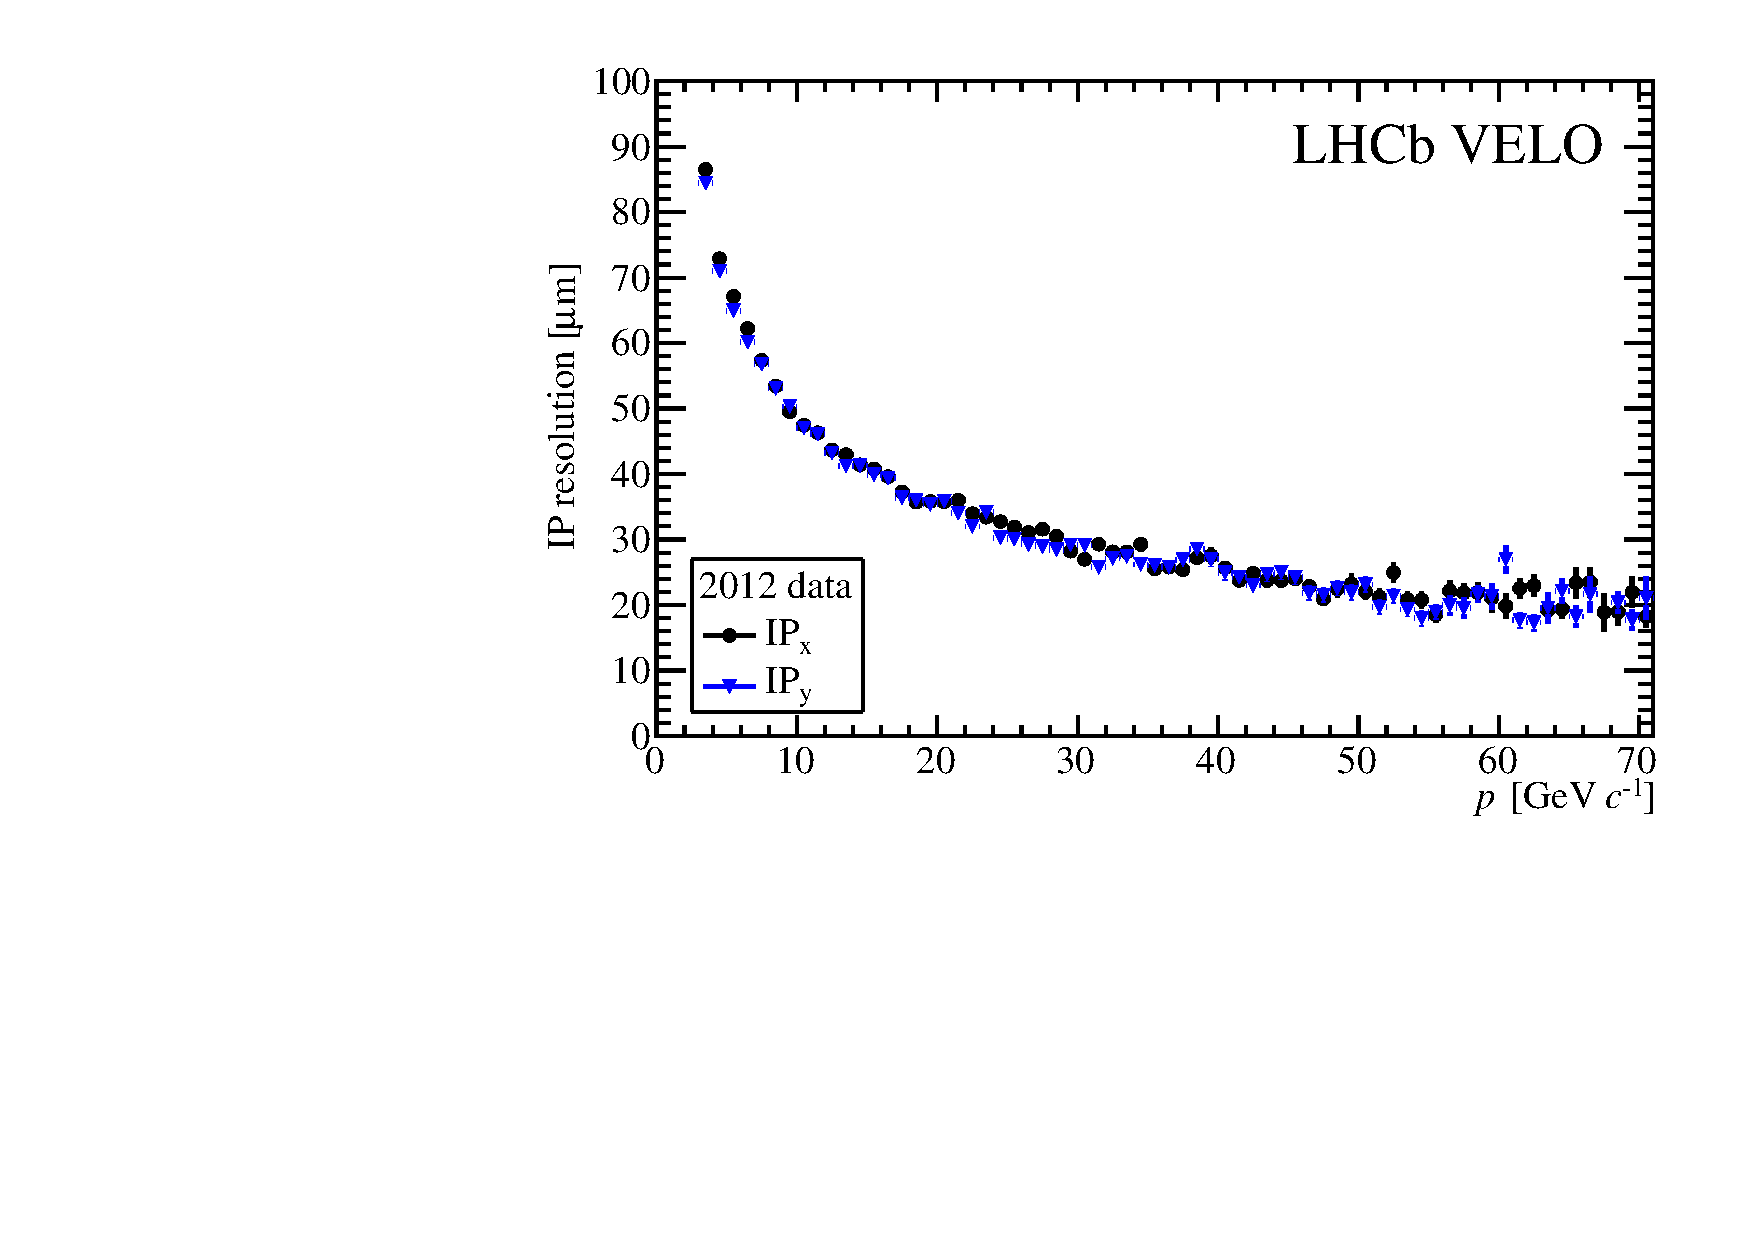
\includegraphics[scale = 0.4]{figs/IPRes-Vs-P-CompareIPxIPy-2012}\label{1}}
  \subfloat[]{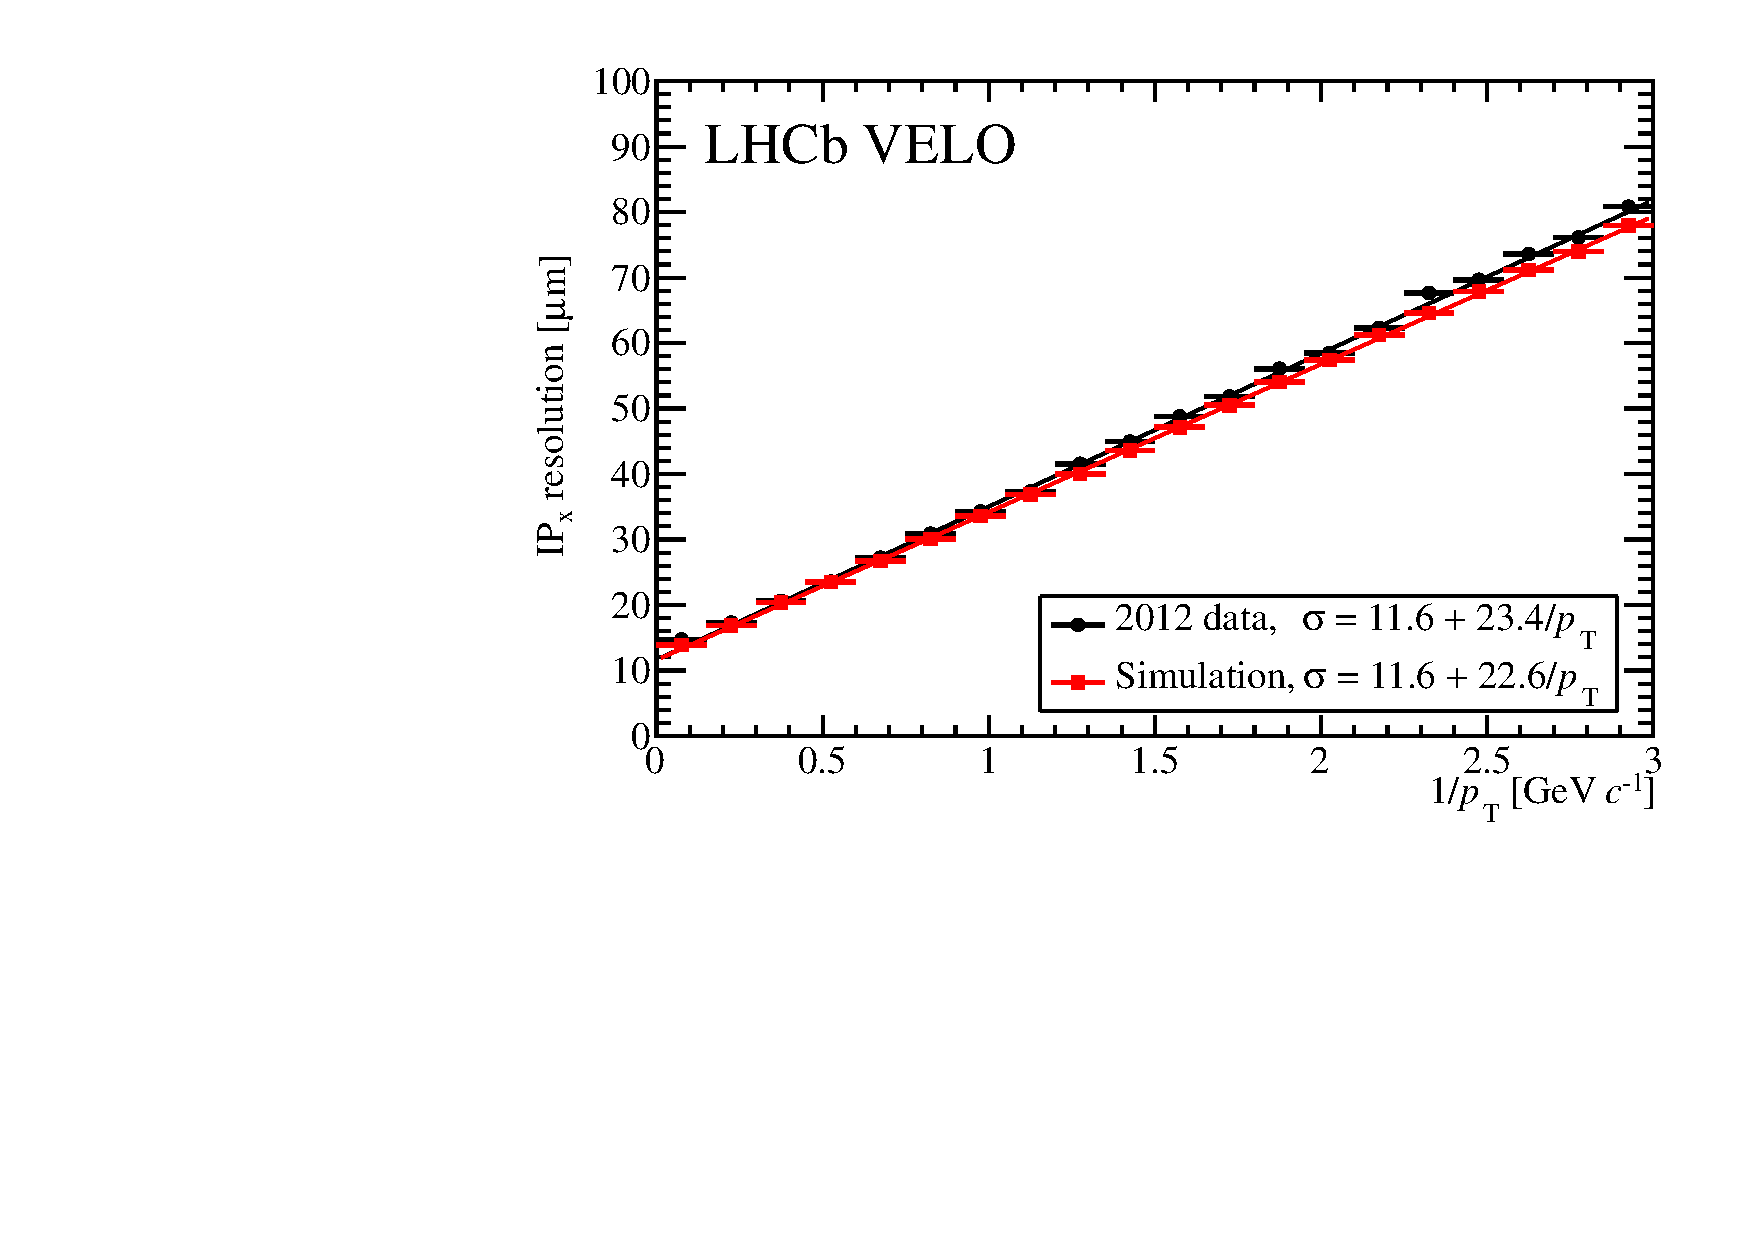
\includegraphics[scale = 0.4]{figs/IPXRes-Vs-InversePT-Compare2012DataToMC}\label{2}}
  \caption{The resolution of $IP_{x}$ and $IP_{y}$ as a function of the momentum of the track, \protect\subref{1}, the resolution of $IP_{x}$ and $IP_{y}$ as a function of $1/P_{T}$, \protect\subref{2} \cite{LHCb-DP-2014-001}.}
  \label{fig:IP}
\end{figure}

\subsection{Measuring the PV position}
A good measurement of the PV position is important for gaining good precision on the FD of a particle. The PV resolution is strongly correlated with the number of tracks, $N$, in an event. At least five tracks are required to form a PV. %The maximum number is around 100.

The resolution of the PV in the $x$, $y$ and $z$ directions is fitted using the function
%% is deduced by randomly splitting the tracks in an event into two sets. The vertex reconstruction algorithm is then applied to each set and vertices in each set which are have a difference in their $z$ position of less than $2\mm$ are deemed to be the same vertex. For each pair of vertices matched between the two sets the residual is calculated. This is repeated for many events and the resulting histograms of residuals in $x,y,z$ is fitted using the function

\begin{equation}
  \sigma_{PV} = \frac{A}{N^{B}} + C,
  \label{eq:pv}
\end{equation}
where $A, B$ and $C$ are constants. The resolution of the PV in $x,y,z$ as a function of $N$ can be seen in~\autoref{fig:PVres}.
\begin{figure}
  \centering
  \subfloat[]{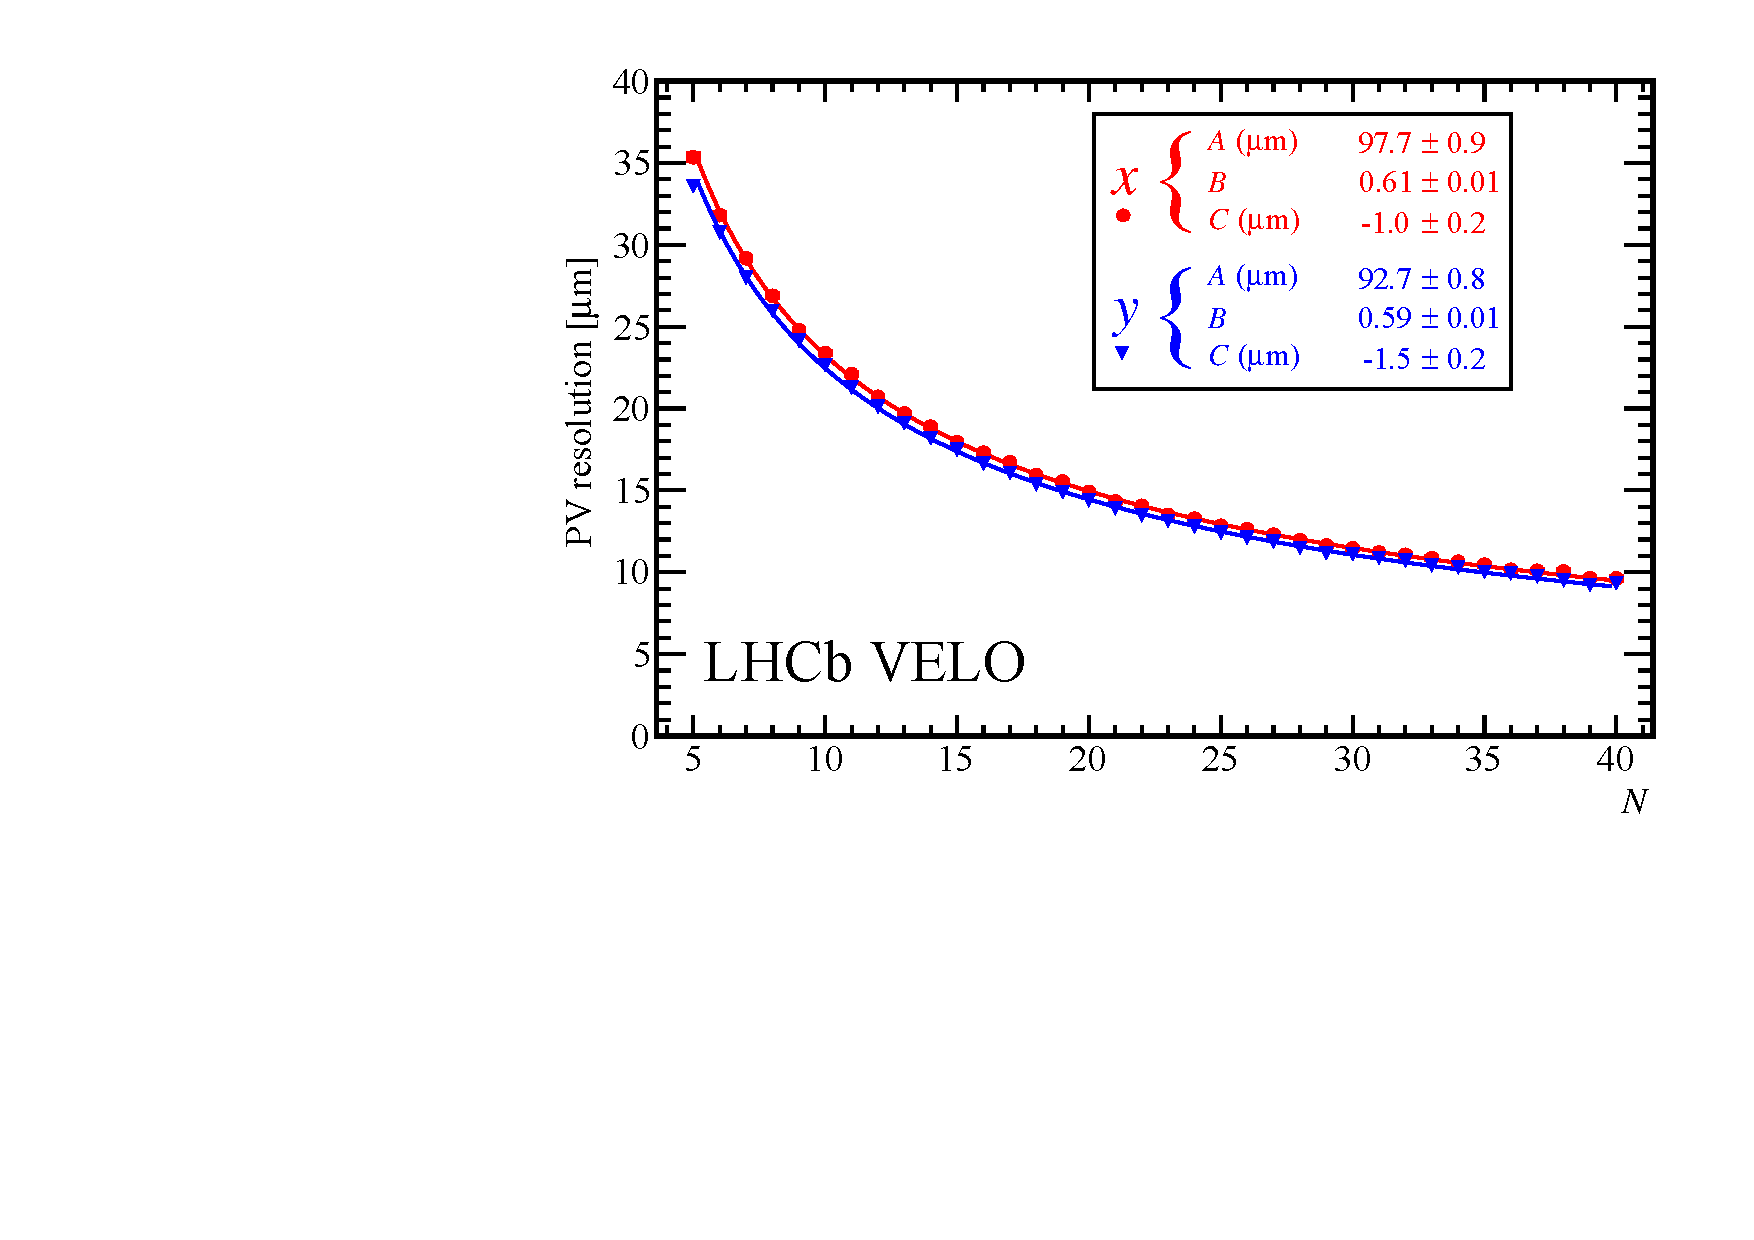
\includegraphics[scale = 0.4]{figs/ResXY_1PV_2011Data}\label{1}}
  \subfloat[]{\includegraphics[scale = 0.4]{figs/ResZ_1PV_2011Data}\label{2}} 
  \caption{The PV resolution in the $x,y$ directions as a function of track multiplicity, $N$, \protect\subref{1}. The PV resolution in $z$ direction as a function of $N$, \protect\subref{2}. The values in the legends refer to the constants in~\autoref{eq:pv} \cite{LHCb-DP-2014-001}.
  }
  \label{fig:PVres}
\end{figure}

\subsection{Reconstructing tracks in the VELO}

The track-finding algorithms in LHCb start in the VELO. Tracks reconstructed in the VELO are then matched with tracks reconstructed from hits in the tracking units further downstream.
The track reconstruction efficiency is defined as the probability that a charged particle passing through the detector (in this case, the VELO) is reconstructed. %This definition of tracking efficiency does not account for interactions with the material, decays in flight and particles that fly outside of the detector acceptance.

The VELO algorithm searches for tracks by looking for clusters in the $R$ sensors consistent with a straight line and then looks for a set of compatible $\Phi$ sensor clusters to reconstruct a trajectory. The minimum number of clusters required to find a track is six (three in the $R$ sensors and three in the $\Phi$ sensors) and the average number of clusters is 11.

The efficiency of the track reconstruction in the VELO is deduced using a tag-and-probe method. Here samples of \jpsi\to\mup\mun decays are used, where one muon is tagged (fully-reconstructed) and the other probe track is partially reconstructed from hits in other parts of the detector. The momenta of the tag and the probe muon are combined to check that it falls within the \jpsi mass window, which is used to confirm the track selection. The VELO efficiency is then obtained by matching the partially reconstructed track to a fully reconstructed track that includes a VELO segment. The absolute efficiency for data for VELO tracks is $\sim$ 98\%. The VELO tracking efficiency observed in the data and in the simulation is shown in~\autoref{fig:velotrack}.


\begin{figure}
  \centering
    \subfloat[]{\includegraphics[scale = 0.35]{figs/Track_Velo_effVsP2011}\label{1}}
      \subfloat[]{\includegraphics[scale = 0.35]{figs/Track_Velo_effVsEta2011.pdf}\label{2}}
    \caption{The tracking efficiency of the VELO for data and simulation as a function of momentum (left) and $\eta$ (right).
  }%note: 2011 data
  \label{fig:velotrack}
\end{figure}

%The discrepancy between data and simulation can be partially explained by certain assumptions made in tracking. Firstly, in the simulation it is assumed that the interaction point is at zero, whereas in data it is offset by 0.4\mm. Secondly the difference in the distance between the two halves of the VELO differ between data and simulation by $\sim$ 150\mum.


\section{The TT station, T station  and track reconstruction}
\label{sec:Tst}
The TT station sits upstream of the dipole magnet and the T stations sit downstream of the magnet. The TT station is roughly 150cm wide and 130cm high and uses silicon micro-strips to detect passing particles. The Inner Tracker (\Gls{IT}) of the T stations is also made of silicon micro-strips and the outer part (the Outer Tracker (\Gls{OT})) of the T stations is made up of straw tubes. The TT, IT and the OT are shown in~\autoref{fig:OT}.
\begin{figure}[h!]
  \centering
  \includegraphics[scale = 0.5]{figs/OuterTracker.png} 
  \caption{The Outer Tracker in the T stations (light blue) made up of straw-modules and the Inner Tracker and TT station (purple) made up of silicon micro-strips \cite{OT}.
  }
  \label{fig:OT}
\end{figure}
Each outer tracker for each T station consists of four layers rotated with respect to the vertical by (0$\degree$, $-$5$\degree$, 5$\degree$, 0$\degree$).

%The rotated layers are referred to as the stereo layers and the non-rotated ones as $x$ layers.

Charged particles must have a momentum of at least 1.5\gevc in order to traverse the magnetic field and reach the T stations. The trajectories of charged particles passing through the detector can be reconstructed from hits in the VELO, T and TT (IT and OT) stations. An example event showing such tracks reconstructed from assigned hits in these stations can be seen in~\autoref{fig:hits}.
\begin{figure}[h!]
  \centering
  \includegraphics[scale = 0.5]{figs/hits} 
  \caption{A display of the reconstructed tracks for an event along with the assigned hits in blue. The insert shows a zoom of the VELO region in the $x$-$y$ plane \cite{det_paper}.
  }
  \label{fig:hits}
\end{figure}

\begin{figure}[h!]
  \centering
  \includegraphics[scale = 0.4]{figs/DOWNUP} 
  \caption{Different types of track in the LHCb detector along with the corresponding magnetic field strength in the $y$ direction \cite{det_paper}
  }
  \label{fig:updown}
\end{figure}
The tracks in LHCb can be characterised into different types, as outlined in~\autoref{fig:updown}. These different track types are:

\begin{description}
\item[Long tracks] which traverse the entire detector. They are defined as tracks which have hits in the VELO and the T stations. Hits in the TT stations are optional. As they traverse the full magnetic field, long tracks offer the most precise momentum measurement and are therefore of most importance to physics analyses. They are also the best understood tracks in terms of efficiency measurements. There are on average 33 long-tracks per event \cite{uksem}. 

\item[Upstream tracks] leave hits only in the VELO and the TT station. This is generally due to the tracks having too low a momentum to reach the T stations. These tracks are not used directly in physics analyses.
%These tracks are only useful for understanding backgrounds in PID algorithms in RICH1 (providing they have a high enough momentum to pass RICH1).

\item [Downstream tracks] like long tracks, are directly used in physics analyses for particles which are long-lived enough to decay outside the VELO, such as $K^{0}_{s}$ and $\Lz$. The reconstruction efficiency of these tracks is poorly understood and part of this thesis focuses on a method to improve this efficiency measurement. There are on average 14 downstream tracks per event.
\item [VELO tracks] pass only through the VELO and are used for PV reconstruction. They are not used directly in physics analyses.
\item[T tracks] pass only through the T stations and tend to be produced in secondary interactions. They are not used directly in physics analyses.  %Again their only use is within the context of RICH2 data treatment for particle identification.
\end{description}

The reconstruction of VELO tracks has already been described. There are two complementary algorithms for adding tracks from downstream detectors to these VELO tracks to make a long track. In the first, so-called forward tracking, the momentum of a particle and its trajectory are entirely determined from a VELO track and a single hit in one of the T stations. Further hits in the T stations which are compatible with this trajectory are then added \cite{forward}. The second algorithm used is referred to as track-matching, where long tracks are made by combining VELO tracks with T tracks, which are found by a stand alone track-finding algorithm \cite{patseed}.

%% Here a track segment is reconstructed in the downstream detectors and then combined with the VELO track. The downstream track segment is formed by requiring that particles leave hits in at least one $x$ and stereo layer in each of the three T stations \cite{match}.

For both algorithms the candidate tracks are combined to form a final set of long tracks. Once combined, hits from the TT station consistent with the trajectory are also added to improve the momentum measurement \cite{tracks}. %The average efficiency to reconstruct long tracks is (97.78 $\pm$ 0.07)\% for 2011 data and (96.99 $\pm$ 0.05)\% for 2012 data \cite{tracks}.

The downstream tracks are reconstructed by taking a stand alone T track and then extrapolating this track through the magnetic field. Once having computed the point at the centre of the magnetic field using the T track, a search for a list of TT measurements making a straight-line with this point is carried out. The main challenges for this method are \gls{ghost} tracks (i.e. hits within the detector which are falsely reconstructed as a track) and the wide window across the TT station within which matching TT measurements must be searched for \cite{downstream}.

%% The efficiency of the downstream track finding algorithm is calculated using simulation. The efficiency for the algorithm to correctly identify a track which has TT and T hits and that is not constructable in the VELO is found to be 46\% Ref.\cite{downstream}. This efficiency increases to 73\% when it is required that the particles reconstructed are daughters of strange mothers produced near the beam line. 

The work described later in this thesis will outline a method to measure the downstream track-finding efficiency using a data-driven method, as a function of $p$ and $\eta$, and will provide a relationship between the downstream tracking efficiency observed in data and the downstream tracking efficiency according to simulation.

%% \section{The \sPlot  technique and $\mathbf{\sWeight}$-ing data}
%% \label{sec:splot}
%% As the following section on the RICH detectors will mention a statistical technique referred to as the \sPlot technique \cite{sPlot}, or \sWeight-ing, the concept is introduced here.

%% The \sPlot technique is used extensively through out this thesis. It is used in cases when one has a merged dataset which consists of data from different sources of data species, namely background and signal. The events in this dataset are assumed to be composed of two different sets of variables. Discriminating variables are those whose distributions are known for background and signal. Control variables are those whose distributions are unknown, or are assumed to be unknown.

%% The \sPlot technique allows the distribution of the control variables for each data species to be deduced by using the species discriminating variable. This method relies on the assumption that there is no correlation between the discriminating variable and the control variable. The discriminating variable used in this thesis is always the mass distribution. The full mathematical description of the \sPlot technique can be seen in Ref. \cite{sPlot}, the key points are outlined here.

%% An unbinned extended maximum likelihood analysis of a data sample of several species is considered. The log-likelihood is expressed as

%% \begin{equation}
%%   \mathcal{L} = \sum^{N}_{e = 1} \left\{\ln \sum^{N_{s}}_{i = 1} N_{i}f_{i}(y_{e})\right\} - \sum^{N_{s}}_{i = 1}N_{i},
%%   \label{eq:ll}
%% \end{equation}

%% where $N$ is the total number of events considered, $N_{s}$ is the number of species of event (i.e. two - background and signal), $N_{i}$ is the average number of expected events for the $i^{th}$ species, $y$ represents the set of discriminating variables and $f_{i}(y_{e})$ is the value of the Probability Density Function (PDF) of $y$ for event $e$ for the $i^{th}$ species. 

%% For the simple (and not particularity practical) case of the control variable $x$ being a function of $y$, i.e. completely correlated, one could naively assume that the probability of a given event of the discriminating variable $y$ being of the species $n$ would be given by

%% \begin{equation}
%%   \mathcal{P}_{n} (y_{e}) = \frac{N_{n}f_{n}(y_{e})}{\sum^{N_{s}}_{k =1} N_{k}f_{k}(y_{e})}.
%% \end{equation}
%% In this scenario the probability would run from 0 to 1.
%% In the case considered in this thesis, where $x$ is entirely uncorrelated with $y$, it can be shown that $\mathcal{P}_{n} (y_{e})$ can be written as

%% \begin{equation}
%%   \mathcal{P}_{n} (y_{e}) = \frac{\sum^{N_{s}}_{j = 1} V_{nj}f_{j}(y_{e})}{\sum^{N_{s}}_{k =1} N_{k}f_{k}(y_{e})},
%%   \label{eq:sw}
%% \end{equation}

%% where $V_{nj}$ is the covariance matrix between the species $n$ and the $j^{th}$ species. The inverse of this covariance matrix is given by the second derivative of -$\mathcal{L}$ in~\autoref{eq:ll}.

%% The quantity in~\autoref{eq:sw} is donated as the \sWeight. In this thesis the species, $n$, in~\autoref{eq:sw} is always the signal. Because of the presence of the covariant derivative the \sWeight of an event can be both positive and negative. The more negative an event is the more likely it is to be background and vice versa for positive \sWeight-s. The signal distribution for the control variable $x$ can then be deduced by histrogramming events in $x$, applying the \sWeight to each event. %Again it is important that the $x$ variable is not correlated with $y$ (that is - the mass distribution).


%% In practice, the \sPlot technique is applied by fitting the background and signal mass distributions in data and using the fitted probability density function (PDF) of the $i_{th}$ species, the total number of events in the data sample, the number of species in the data sample (i.e. two) and the number of average events expected for the $i_{th}$ species, to deduce a weight for each event. These weights range between -1 and 1 .

   
\section{The RICH detectors}
\label{sec:rich}
The main role of the \Gls{RICH} is to provide identification for the charged hadrons $\pi,\kaon$ and \proton. It also provides information on the charged leptons $e$ and $\mu$ which complement the information provided by the calorimeter and muon systems.

%There are two RICH detectors, RICH1 and RICH2, as seen in~\autoref{fig:dec}. Between the two detectors a momentum range of $\sim$1-100\gevc is covered

The momentum of a particle is highly correlated to the polar angle $\theta$, with high momentum particles having a smaller angle. The RICH1 detector system is placed just after the VELO and provides identification for particles with a low momentum range of 2-40\gevc. The RICH2 detector system is placed between the T stations and the first \gls{muonstation}, M1, and covers a momentum range of 15--100\gevc. The RICH2 detector system is placed further downstream, as the higher momentum particles are less affected by the magnet.

The RICH functions on the basis that if a particle travels faster than the speed of light in a medium it will emit \v{C}erenkov radiation. The angle of this radiation is related to the speed of the particle and the refractive index of the medium.  By measuring the \v{C}erenkov angle $\theta_{c}$, the particle mass can be deduced through the relation

\begin{equation}
  \cos\theta_{c} = 1/\beta n  = E/pn =  \frac{\sqrt{m^{2} + p^{2}}}{pn}.
\end{equation}

The radiators used in RICH1 are silica aerogel and $C_{4}F_{10}$. The aerogel has a very low density and high refractive index which makes it ideal for very low momentum particles with momenta $\sim$ \gevc. The aerogel is placed just after the VELO and the rest of the RICH1 is filled with $C_{4}F_{10}$. The optical system in both RICH detectors is similar. A primary spherical tilted focusing mirror and a plane secondary mirror focus and direct the \v{C}erenkov light on to a plane of hybrid photon detectors (HPDs), as shown in~\autoref{fig:rich1}.

%These mirrors focus the \v{C}erenkov radiation of a particle on to the hybrid photon detectors (HPD), as seen in~\autoref{fig:rich1}.

\begin{figure}[h!]
  \centering
  \includegraphics[scale = 0.9]{figs/RICH1diagram.png} 
  \caption{The optical set-up for the RICH1 detector \cite{rich1dia}.
  }
  \label{fig:rich1}
\end{figure}

%There are 2 planes of HPDs in each RICH, with a total of 198 HPDs in RICH1 and 288 in RICH2. 

\subsection{The particle identification algorithm}
A good understanding of the performance of the Particle IDentification (\Gls{PID}) of the RICH is important for the analyses described in this thesis. A precise understanding of the performance  allows the efficiency and mis-identification (mis-id) rate of tracks to be calculated after the RICH information has been applied to the data candidates. To identify effectively the particle type of a track in the RICH, an overall event log-likelihood algorithm is calculated, taking into account all possible hypotheses for all tracks in the event. %s for both rich detectors simulation.

%applied which includes all of the tracks in an event and the information from both RICH detectors simultaneously.

The likelihood minimisation procedure starts by assuming all particles are pions, as pions are the most abundant particle type. The overall event likelihood is calculated from the distribution of the photon hits (which will form rings referred to as \v{C}erenkov rings) along with the event's associated tracks and their errors, assuming the pion mass hypothesis for every track. The mass hypothesis of each track is then changed, one track at a time, whilst leaving the hypothesis for every other track in the event unchanged. The mass hypotheses for $e$, $\mu$, $K$ and proton are applied and the change in mass hypothesis which gives the largest increase in the event likelihood is identified. This method is repeated until no improvement in the event likelihood can be found and thus each track has been set to its preferred hypothesis. Some modifications are made to the logic described above in order to reduce CPU time. The final output of this algorithm is a variable for each track in an event which shows the difference in the total event log-likelihood when the mass hypothesis of the track in question is changed from a pion to $e$, $\mu$, $K$ and proton. These variables are referred to as e.g. \gls{dllkpi}  = $\Delta \text{Log}(\kaon - \pi)$, \gls{dllppi} = $\Delta \text{Log}(\proton - \pi)$ and \gls{dllmupi} = $\Delta \text{Log}(\mu - \pi)$. % and \dllepi = $\Delta \text{Log}(e- \pi)$.
\subsection{The PID performance}
\label{sec:pidperf}
%% The PID performance can be investigated with data, using decays with isolated tracks, whereby the \v{C}erenkov ring from a track does not overlap with other rings. This allows the \v{C}erenkov angle to be uniquely predicted.

The performance of the PID is assessed using data candidates which have been selected without using PID information. Thus decays are needed whereby the individual daughter states can be reconstructed with very little background, using kinematic information alone. The decays chosen include the channels $\PLambda^{0}\to\proton\pim$ and $D^{*+} \to D^{0}(\kaon^{-}\pip)\pip$. These decays have a high purity as can be seen~\autoref{fig:pidcalib}.
\begin{figure}[h!]
  \centering
  %  \subfloat{\includegraphics[scale = 0.23]{figs/kspipi.png}\label{1}}
  \subfloat{\includegraphics[scale = 0.23]{figs/lambdabppi.png}\label{1}}
  \subfloat{\includegraphics[scale = 0.23]{figs/dkpi.png}\label{2}}
  \caption{Fitted invariant mass distributions for $\PLambda^{0}\to\proton\pim$, \protect\subref{1}, and $D^{0}\to \kaon^{-}\pip$, \protect\subref{2} \cite{LHCb-DP-2012-003}.}
  \label{fig:pidcalib}
\end{figure}
The remaining background is removed using the \sPlot technique \cite{sPlot}, which assigns a so-called sWeight (which can be positive or negative) to each event, depending on how signal-like the event is deemed to be.  The \sPlot technique is summarised in~\autoref{sec:splot}.

Using these control samples, the $\text{DLL}_{X\pi}$ distributions are considered for each track type. It is then possible to study the discriminating power of particular PID requirements. The discriminating power of the selection cuts \dllkpi$>0$ and \dllkpi$>5$ placed on tracks with a kaon mass hypotheses can be seen in~\autoref{fig:pid1}\protect\subref{1}. Here the efficiency of these cuts on kaons is shown along with the misidentification of pions as kaons.
 The discriminating power of the selection cuts \dllppi$>0$ and \dllppi$>5$ on tracks with a proton mass hypotheses can be seen in~\autoref{fig:pid1}\protect\subref{2}, along with the mis-id rate of pions to protons and finally the efficiency is shown for $\dllpk>0$, $\dllpk>5$ along with the mis-id rate of kaons to protons in~\autoref{fig:pid1}\protect\subref{3}. In~\autoref{fig:pid1}\protect\subref{3} the variable \dllpk is formed using the relation
\begin{equation}
  \dllpk = \dllppi - \dllkpi.
\end{equation}

\begin{figure}[h!]
  \centering
  \subfloat[]{\includegraphics[scale = 0.8]{figs/kpi_det.png}\label{1}}
      \subfloat[]{\includegraphics[scale = 0.8]{figs/ppi_det.png}\label{2}}\\
      \subfloat[]{\includegraphics[scale = 0.8]{figs/pk_det.png}\label{3}}
      \caption{The kaon efficiency and the misidentification rate for pions as kaons for different PID cuts (filled and hollow markers) \protect\subref{1}, the proton efficiency and the misidentification rate for pions as protons for different PID cuts (filled and hollow markers), \protect\subref{2} and the proton efficiency and the misidentification rate for kaons as protons for different PID cuts (filled and hollow markers), \protect\subref{3} \cite{LHCb-DP-2012-003}.}
  \label{fig:pid1}
\end{figure}

The \v{C}erenkov angle as a function of momentum for tracks passing through the $C_{4}F_{10}$ radiator is shown in~\autoref{fig:cheren}
\begin{figure}[h!]
  \centering
  \includegraphics[scale = 0.9]{figs/cherenkov_angle.png} 
  \caption{Reconstructed \v{C}erenkov angle as a function of track momentum in the $C_{4}F_{10}$ radiator \cite{LHCb-DP-2012-003}.
  }
  \label{fig:cheren}
\end{figure}




%% \begin{figure}[h!]
%%   \centering
%%   \includegraphics[scale = 0.9]{figs/ppi_det.png} 
%%   \caption{The proton efficiency and the misidentification rate for pions as protons for different PID cuts (filled and hollow markers) \cite{LHCb-DP-2012-003}.}
%%   \label{fig:pid2}
%% \end{figure}

%% \begin{figure}[h!]
%%   \centering
%%   \includegraphics[scale = 0.9]{figs/pk_det.png}
%%     \caption{The proton efficiency and the misidentification rate for kaons as protons for different PID cuts (filled and hollow markers) \cite{LHCb-DP-2012-003}.}
%%     \label{fig:pid3}
%% \end{figure}


%% The dependence of the efficiency on momentum and the mis-id rates for varying combinations of pion, proton and kaons can be understood from the variation of $\theta_{c}$ with momentum shown in~\autoref{fig:cheren}. As shown in~\autoref{fig:cheren} the seperation between the kaon and proton hypothesis is less clear for softer protons. Due to this, harder initial cuts are often placed on the proton momentum during off-line analysis. The discriminatory power of a PID cut is also a function of the event multiplicity and $\eta$. 

%% \subsection{The PID calib package}

%% The PID calib package is a collection of files used within the LHCb software which allow the efficiency and mis-identification rates to be calculated for any momentum cut for a particular $\text{DLL}$ variable. These values are calculated using the control channels discussed previously. This package can also be used to reproduce the number of events per PID value for a selected mass hypothesis. These DLL distributions provided by PID calib are binned in terms of momentum, $\eta$ and track multiplicity. The PID calib package provides the $\text{DLL}$ variables \dllppi, \dllkpi \dllmupi and \dllepi. %To deduce the difference in the  log likelihood of a particle with respect to a particle that is not a pion a linear combination of the above $\text{DLL}$ variables can be taken. 

\section{Muon identification}
\label{sec:muonID}
The selection of muons is performed using information from the five muon detector stations M1--5. Each station is divided up into four regions R1--4, all of which cover roughly the same acceptance, as shown in~\autoref{fig:muonst}. The granularity of the station in each region R1--4 reflects the particle density in that region. There is also increased granularity in the $x$ direction, as this is the plane in which particles are bent by the magnetic field.

The M1 station is placed before the \Gls{ECAL} and stations M2--5 are placed downstream of the ECAL. Stations M2--5 are interleaved with 80cm thick iron absorbers. These iron absorbers along with the muon stations M2--5 allow the identification of penetrating muons.
%The final iron filter in~\autoref{fig:muonst} is placed in order to reduced backscattering in the M5 station. 

\begin{figure}[h!]
  \centering
  \includegraphics[scale = 0.9]{figs/MuonStations.png} 
  \caption{The five muon stations (a) (the muon filters refer to iron absorbers - see text) and (b) the station layout in regions R1--4 \cite{muon}.
  }
  \label{fig:muonst}
\end{figure}


%% \subsection{The L0 muon trigger}
%% \label{sec:L0muon}
%% As discussed in~\autoref{sec:L0trig}, the information provided by the muon stations is used in the \Gls{L0} hardware trigger. The L0 muon trigger performs a standalone reconstruction of tracks, requiring hits in all five stations, which allows the $P_{T}$ of a track to be estimated using the hardware alone. The estimation of the track's $P_{T}$ is done by combining tracks in stations M2-5 with hits from M1. The track direction after deflection by the magnetic field can then be determined . The positioning of the M1 further upstream allows a better resolution of the $\pt$ of a given track in the L0 trigger (reducing the resolution from $\sim$35\% to $\sim$25\%) but the M1 station is not used in the high level trigger or off-line reconstruction of tracks.

%Because the muon stations are used in the L0 trigger they are required to send information to the trigger having identified collision events within a time window of 25 $ns$. 

%% Firstly a track is verified in the four stations, M2-5, by searching within suitable areas relative to the interaction point. Then the position of the hits in M2 and M3 are used to predict the position of hits in M1. If a hit is found in M1 within a suitable region the next step is to estimate the \pt of this track to verify whether or not it should pass the trigger.  This done by using the hits in M1 and M2 to find the track direction after deflection by the magnetic. This direction, combined with its impact point at the magnetic centre and the average $pp$ collision point, are used to make a quick estimate of the $\pt$ \cite{muon}. The presence of the M1 further upstream allows a better resolution of the $\pt$ of a given track in the L0 trigger (reducing the resolution from $\sim$35\% to $\sim$25\%) but it is not used in the high level trigger or offline reconstruction of tracks.


\subsection{The efficiency of the muon stations}
As the L0 algorithm requires hits in all five muon stations and an overall efficiency of $>95$\% is desirable, the efficiency of each individual station must be at least 99\%. This is achieved by having a good time resolution and a high detector redundancy. This redundancy is realised by having two independent readouts in many of the stations/regions and requiring a hit in at least one of them and the time resolution to be better than 4ns. All regions of all muon stations fulfil the $>99$\% requirement. %, giving a total muon reconstruction efficiency of $>$95\%. %The efficiency for each muon station as a function of station region is shown in~\autoref{tab:muoneff}.

%% The efficiency of the stations M2-5 are measured by looking at the events which weren't triggered in the HLT or L0 triggers by the muon system. Tracks are then reconstructed using all muon systems minus the one under investigation. These M-tracks are also required to match to good quality high momentum T-tracks. The predicted positions of hits in the M station under investigation, deduced by extrapolation the track already reconstructed from the other stations, are then compared to hits with the M station underinvestgaion in order to deduce the efficiency.

%% For the case of M1 a similar procedure is followed but this time the data comes from \jpsi \to \mup\mun decays, where the muon considered is the one that didn't fire the L0 trigger. This data can be used in the case of M1 because the M1 information is not used in the HLT or offline track reconstructions.


%% \begin{table}
%%   \centering
%%   \hspace*{-0.5cm}
%%   \includegraphics[scale = 0.5]{figs/muonefftab}
%%   \caption{The efficiency to correctly reconstruct a track made by a muon in each region of each muon station. Errors indicate statistical and systematic errors respectively \cite{muon}.}
%%   \label{tab:muoneff}
%% \end{table}

%% The main source of systematic error on the efficiency comes from the modelling of backgrounds whilst calculating the efficiency. 
\subsection{The muon identification procedure}
The  off-line muon identification strategy can be split into three steps \cite{muonID}
\begin{description}
  \item[IsMuon:] A binary selection of muon candidates based on the penetration of the muon candidates through the calorimeters and iron filters is parameterised by the boolean IsMuon variable. There are also momentum requirements, depending on which muon stations have been traversed.  This provides high efficiency, while reducing the misidentification probability of hadrons to the percent level.    
  \item[muDLL:] Based on the pattern of hits around the extrapolation to the different muon stations of the trajectories of charged particles reconstructed in the tracking system, the logarithm of the ratio between the muon and non-muon hypotheses is constructed and used as a discriminating variable, referred to as muDLL. %The pattern of hits around the extrapolated track position allows a computation  of a likelihood for a muon and non-muon hypothesis. The logarithm of the ratio between the muon and non-muon likelihoods gives the discriminating variable muDLL. %in each muon station for IsMuon=true are shown in~\autoref{tab:muonID}. The tracks must also appear in the correct Field of Interest (FOI), i.e. within a certain distance of the extrapolated upstream tracks position in the muon stations.
  \item[$\mathbold{DLL_{\mu\pi}}$:] The RICH information, along with information from the calorimeter, is combined with muDLL to give the discriminating variable \dllmupi.
\end{description}

%% \begin{table}
%%   \centering
%%   \begin{tabular}{l|c}
%%     \hline
%%     Momentum range/(\gevc) & Muon stations\\
%%     \hline
%%     3$<p<$6 & M2 and M3\\
%%     6$<p<$10 & M2 and M3 and (M4 or M5)\\
%%     $p>$10 & M2 and M3 and M4 and M5\\
%%     \hline
%%   \end{tabular}
%%   \caption{Muon stations required to trigger the IsMuon decision as a function of momentum range.}
%%   \label{tab:muonID}
%% \end{table}

\subsection{Efficiency of the muon ID procedure}
The efficiency of the muon selection process is extracted from data, using \jpsi\to\mup\mun decays combined with tag-and-probe techniques. The calculation of the mis-id rates of kaons, pions and protons to muons is performed using the decays outlined in~\autoref{sec:pidperf}. The efficiency for IsMuon, $\epsilon_{IM}$, is shown in~\autoref{fig:isMuon}, along with the mis-id rates as a function of momentum and in ranges of transverse-momentum.

%% the efficiency for finding tracks within the the FOI and which meet the momentum requirements in~\autoref{tab:muonID},

\begin{figure}
  \centering
  \subfloat[]{\includegraphics[scale = 0.3]{figs/Muon1a.png} \label{1}}      
  \subfloat[]{\includegraphics[scale = 0.3]{figs/Muon1b.png}\label{2}}\\
  \subfloat[]{\includegraphics[scale = 0.3]{figs/Muon2a.png}\label{3}}
  \subfloat[]{\includegraphics[scale = 0.3]{figs/Muon2b.png}\label{4}}\\      
  \caption{
 IsMuon efficiency and misidentification probabilities, as a function of momentum and in ranges of transverse-momentum: efficiency of IsMuon on muons, $\epsilon_{IM}$, \protect\subref{1}, IsMuon mis-id rate ($\proton\to\mu$), \protect\subref{2}, IsMuon mis-id rate ($\pion\to\mu$), \protect\subref{3}, and IsMuon mis-id rate ($\kaon\to\mu$), \protect\subref{4} \cite{muonID}.
  }
  \label{fig:isMuon}
\end{figure}

There is a weak efficiency dependence on transverse-momentum. The reason for a more dramatic loss of efficiency for low $P_{T}$ muons is due to the scattering of tracks out of the detector. The mis-id rate also falls with increased transverse-momentum. This is because a higher $P_{T}$ for a given momentum corresponds to a larger polar angle and the track then traverses lower occupancy detector regions \cite{muonID}.

The efficiency of the \dllmupi variable on muons, compared to the mis-id rate for kaons and pions, along with the equivalent distributions for the muDLL variable alone, are shown in~\autoref{fig:dllmupi}.
\begin{figure}[!h]
  \centering
      \subfloat[]{\includegraphics[scale = 0.26]{figs/muontot.png} \label{1}}           \subfloat[]{\includegraphics[scale = 0.26]{figs/muontot1.png}\label{2}}\\
        \caption{Efficiency of selecting muons against the efficiency for selecting pions for the \dllmupi and muDLL variables, \protect\subref{1}. Efficiency of selecting muons against the efficiency for selecting kaons for the \dllmupi and muDLL variables, \protect\subref{2}.
  }
  \label{fig:dllmupi}
\end{figure}
The variables most used in the work presented in this thesis are the IsMuon and $\dllmupi$ variables in combination. 

\section{Simulation}
The analyses described in this thesis rely on an accurate simulation of the physics within the detector, and of the detector itself, in order to correctly model the detector output. The simulation of the detector output can be split into two stages; simulation of the particle decays; and simulation of the detector and the particles interactions with it. In the remainder of this thesis, the simulation of the particles themselves with no detector present is referred to as the generator-level simulation.

The first stage of simulation is to generate $pp$ collisions. These are generated using Pythia 6.4\cite{pythia6} and Pythia 8.1 \cite{pythia8}, which produce sets of outgoing particles produced in the interactions between two incoming particles \cite{pythia6}. The simulated $b\overline{b}$ quark pair is hadronised repeatedly until the relevant $b$-hadron is produced, which for much of  the simulation used in this thesis would be a \Lb baryon \cite{Sam}. Once the relevant $b$-hadron has been simulated, its decay is described by the EvtGen package \cite{Lange:2001uf} which allows for the implementation of form factors and other different physics models. The final state radiation is generated using Photos \cite{photos}. All of these programs, Pythia, EvtGen and Photos are combined to create generator-level simulation. The LHCb detector and the material interactions of particles with the detector are simulated using the Geant4 \cite{Geant4} tool-kit. In the remainder of this thesis, simulation which includes both the detector and the physics simulation is referred to as reconstructed simulation or just simulation.         

%% These $pp$ collisions are generated in almost equal amounts by Pythia 6.4 \cite{pythia6} and Pythia 8.1 \cite{pythia8}.

%% The analysis described in this thesis makes use of simulated data (or pseudodata) events in several areas. Generation of simulated data makes use of existing generic open-source
%% simulation software in a specific LHCb configuration [68].
%% In the first step, pp collision events are generated using Pythia 6.4 [69] and 8.1 [70] in
%% approximately equal measures. The simulated bb quark pair is hadronised repeatedly until
%% a target b hadron4 is produced. The decay of the b hadron is described by EvtGen [71]
%% and final-state radiation is generated using Photos [72]. The particles are then passed
%% through a full simulation of the LHCb detector where the detector model, and the material
%% interactions are implemented using Geant4 [73]. The data from the simulated detector
%% is then stored and reconstructed as if it were real data.
\clearpage

\input{K_{s}_tracking_efficiency}
\chapter{Selection and backgrounds in the \boldmath{\Lbpi} analysis}
\label{chap:sel}
The \Lb is a heavy baryon containing a bottom quark. The decay mode \Lbpi is a $b\to d$ \Gls{FCNC} transition and can therefore only occur at loop level in the SM. In new physics models, new heavy particles can contribute and can significantly change the branching fraction of this process.

In this chapter, an outline of the selections used to increase the fraction of signal events with respect to the background is presented, along with the types of backgrounds considered. In the next chapter, the multivariate analysis techniques used to further reduce background are presented. In \autoref{chap:mass} there will be a discussion of the fit models used and the efficiencies of the selections applied and finally the results of this analysis are presented in \autoref{Sec:Results}.

In this chapter in \autoref{sec:overview}, a brief reiteration of the motivation for searching for \Lbpi is presented, along with an outline of the analysis method. This is followed by a summary of the data and simulation samples used in this analysis in \autoref{sec:datasiminto}, and then the details of the initial selection applied to increase the signal fraction of events with respect to the background in \autoref{Sec:Pre}. The agreement between data and simulation samples is discussed in \autoref{sec:datasim}. The selections used to remove decays from $B$ reflections, i.e. decays with a mis-identified particle that can accumulate at a certain $B$ mass, and background from the Cabibbo-favoured channel \LbK, are discussed in \autoref{Sec:backgrounds}. Finally, there is a discussion of partially reconstructed backgrounds in \autoref{Sec:partreco}. %various multi-variant analysis techniques usedt o reduced background in X, Y.

This analysis was performed blind, meaning that events within the signal region of the \Lbpi mass spectrum were removed from the dataset during all selection processes outlined in this chapter and during the optimisation process outlined in \autoref{chap:bdt}. Therefore, all plots of the \Lbpi mass spectrum in chapters \ref{chap:sel}--\ref{chap:mass} do not show the signal region.

\section{Overview}
\label{sec:overview}
The aim of the analysis presented in the next four chapters is to measure the \Lbpi branching fraction. The \Lbpi decay mode has never been observed and neither has any other baryon decay mediated by a $b\to d$ transition. The \Lbpi branching fraction is measured relative to the resonant decay mode \Lb\to\proton\pim\jpsi(\to\mumu), which has already been observed \cite{LHCb-PAPER-2014-020}. It is desirable to measure the branching fraction relative to the branching fraction of another decay with the same final state, as many sources of systematic uncertainty cancel. For example the absolute number of \Lb baryons produced within LHCb does not affect the ratio of \BF(\Lbpi)/\BF(\Lb\to\proton\pim\jpsi(\to\mumu)). The \Lb\to\proton\pim\jpsi(\to\mumu) channel is hereafter denoted simply \Lbpijpsi. % is an ideal candidate as it has an identical final state as that of \Lbpi.

%% The Feynman diagrams for the \Lbpi decay were shown in \autoref{fig:boxpeng}\protect\subref{FD:1}, \protect\subref{FD:3} in \autoref{sec:bdll} in \autoref{chap:theory}. The \Lbpi penguin diagram is shown again in \autoref{Fig:FD}, alongside the diagram for the hadronic decay mode \Lbpijpsi.  For both the \Lbpi and \Lbpijpsi decay modes, the proton and pion come from strongly decaying $N^{*}$ resonances.
The Feynman diagram for the \Lbpi decay is shown in \autoref{fig:boxpeng}\protect\subref{FD:1} and the diagram for the hadronic decay mode \Lbpijpsi is shown in \autoref{Fig:FD} .  For both the \Lbpi and \Lbpijpsi decay modes, the proton and pion can come from strongly decaying $N^{*}$ resonances.

\begin{figure}[!ht]%\def\nh{0.5\textwidth}
  \centering
 %% \hspace*{-2.4cm}
 %%  \subfloat[]{\includegraphics[clip=true, trim =10mm 150mm 0mm 0mm, scale = 0.47]{figs/Lb_peng_Huge}\label{FD:1}}
%  \subfloat[]{
    \includegraphics[clip =true, trim = 10mm 170mm 0mm 0mm, scale = 0.57]{figs/Lb_jpsi_HUGE}%}\label{FD:2}
  %% \caption{Feynman diagrams for the signal channel \Lbpi \protect\subref{FD:1},  and the resonant decay \Lbpijpsi \protect\subref{FD:2}.}
    \caption{Feynman diagram for the decay \Lbpijpsi.}
  \label{Fig:FD}
\end{figure}

%%%%%%%%%%%%%%%%%%%%%%%%%%%%%%%%%%%%%%%%%%%%%%%%%%%%%%%%%%%%%%%%%%%%%%%%%%
%% The diagram for the Cabibbo favoured decay mode \LbK can be formed by replacing the $d$ quark in \autoref{Fig:FD}\protect\subref{FD:1} with an $s$ quark.  Thus the ratio of branching fractions, $\BF(\Lbpi)/\BF(\LbK)$, is proportional to the ratio of the CKM matrix elements ${|\frac{\Vtd}{\Vts}|}^{2}$. Together with the $\LbK$ and $\Lbpi$ form factors, a measurement of this branching fraction ratio will therefore allow ${|\frac{\Vtd}{\Vts}|}^{2}$ to be computed and hence a test of the Minimal Flavour Violation (MFV) hypothesis to be made.  This hypothesis predicts that the ratio ${|\frac{\Vtd}{\Vts}|}^{2}$ should be the same in NP models as in the SM. Further measurements of ${|\frac{\Vtd}{\Vts}|}^{2}$ are of interest given the hints of some tension in the CKM unitarity condition that is observed following recent improvements in lattice calculations \cite{vtdvts}. This tension is shown in \autoref{fig:vtdvts}. One of the values of the ratio $|\frac{\Vtd}{\Vts}|$ shown in \autoref{fig:vtdvts} is calculated using the branching fraction ratio $\BF(\Bu\to\pip\mumu)/\BF(\Bu\to\Kp\mumu)$, which was measured using LHCb data in Ref.\cite{LHCb-PAPER-2012-020}.linded


%% \begin{figure}
%%   \centering
%%   \includegraphics[scale = 0.5]{figs/vtdvts.png}
%%   \caption{The values of \Vtd, \Vts and $|\Vtd/\Vts|$ given by tree-level and different loop-level measurements.}
%%   \label{fig:vtdvts}
%% \end{figure}

%%%%%%%%%%%%%%%%%%%%%%%%%%%%%%%%%%%%%%%%%%%%%%%%%%%%%%%%%%%%%%%%%%%%%%%%%%%%%%%%%%%%%%%%%%%%%%


\autoref{tab:bfcomp} shows the comparison of the branching fractions of various decays of the form $\frac{H_{b}\to X_{q}\mu\mu}{H_{b} \to X_{q} \jpsi (\to\mu\mu)}$, where $H_b$ is a hadron containing a $b$-quark and $X_{q}$ is any hadron. The majority of the ratios, $\frac{H_{b} \to X_{q} \jpsi (\to\mu\mu)}{H_{b}\to X_{q}\mu\mu}$, in \autoref{tab:bfcomp}, are of order 100. Taking the ratio between the \Lbpijpsi and \Lbpi branching fractions  to also be of order 100, the 2000 \Lbpijpsi decays observed in 3\invfb of LHCb data in Ref.~\cite{LHCb-PAPER-2014-020} would then lead to an expectation of $\sim$ 10--20 \Lbpi signal events, depending on the relative efficiencies between the \Lbpi and \Lbpijpsi channels. If the ratio of the \Lb decay modes, $\frac{\Lb\to\PLambda\mup\mun}{\Lb\to\PLambda\jpsi}$  is used however, an event yield of 30--60 is expected. In either case, given the small number of signal events expected, the primary challenge for this analysis is the reduction of backgrounds. The branching fractions for the decays \Lbpijpsi and \LbKjpsi are also shown in \autoref{tab:bfcomp}. There is currently no branching fraction measurement for the decay \LbK, although it is an ongoing LHCb analysis at the time of writing. Once the \LbK analysis at LHCb is completed, the \LbK and \Lbpi branching fractions will be combined to deduce the ratio, $\mathcal{R}$, between them. Note that there is little to gain by deducing the \LbK and \Lbpi branching fractions in a combined analysis (which would allow for the cancellation of some systematic uncertainties when calculating $\mathcal{R}$) as the error on $\mathcal{R}$ will be statistically dominated due to the limited statistics available, particularly in the \Lbpi channel. As such, the work outlined in this thesis only measures the branching fraction measurement for \Lbpi and does not attempt to calculate $\mathcal{R}$.  % The branching fractions for the \Lbpijpsi decay, and the Cabibbo-favoured decay \LbKjpsi, are also shown


\begin{table}

  \centering
  \begin{tabular}{l|c|c}
    %% \hline
    %% \BdToJPsiKst  &  (1.32$\pm$ 0.06) $\times$ $10^{-3}$\\
    %% \BdToKstmm & (1.05 $\pm$ 0.10) $\times$ $10^{-7}$\\
    \hline
    Decay& Branching Fraction & Ratio of branching fractions\\
    &&     $\jpsi\to\mumu/\mu\mu$\\
    \hline
    $\Bd\to\Kstarz \mup\mun$ & (1.05 $\pm$ 0.10) $\times$ $10^{-6}$ & \multirow{2}{*}{74.9$\pm$7.9}\\
    $\Bd\to\Kstarz \jpsi$ & (1.32 $\pm$ 0.06) $\times$ $10^{-3}$ &\\
    \hline
    $\Bu\to\Kp \mup\mun$ & (4.43$\pm$0.24)$\times 10^{-7}$ & \multirow{2}{*}{137.2$\pm$8.6}\\
    $\Bu\to\Kp \jpsi$ & (1.02$\pm$0.03)$\times 10^{-3}$ & \\
    \hline
    $\Bd\to\pip\mup\mun$ & (2.3$\pm$0.6)$\times 10^{-8}$ &  \multirow{2}{*}{106 $\pm$ 30}\\
    $\Bd\to\pip\jpsi$ & (4.1$\pm$0.4)$\times 10^{-5}$ &\\
    \hline
    $\Lb\to\Lz\mup\mun$ & (1.1$\pm$0.3) $\times 10^{-6}$& \multirow{2}{*}{34$\pm$12}\\
    $\Lb\to\Lz\jpsi$ & (6.2$\pm$1.4) $\times 10^{-4}$&\\
    \hline
    $\Lbpijpsi$ & $(2.6\pm^{+0.5}_{-0.4}) \times 10^{-5}$& ---\\
    \hline
    $\LbKjpsi$ & $(3.0\pm^{+0.6}_{-0.4}) \times 10^{-4}$& ---\\
    \hline
    
  \end{tabular}
  \caption{Comparison of branching fractions between the $\mumu$ and $\jpsi$ channels for various decays. The ratio between the resonant and non-resonant channels is estimated assuming that $\BF(\jpsi\to\mumu) = 0.0596 \pm 0.0003$. All values for the branching fractions are taken from Ref.\cite{pdg}, with the exception of the \Lbpijpsi and \LbKjpsi branching fraction measurements, which are taken from Refs~\cite{LHCb-PAPER-2014-020} and \cite{LbKjpsi} respectively.}
  \label{tab:bfcomp}
  
\end{table}

 %%%%%%%%%%%%%%%%%%%%%%%%%%%%%%%%%%%%%%%%%%%%%%%%%%%%%%%%%%%%%%%%%%%%%%%%%%
\cleardoublepage
%% METHOD
%%%%%%%%%%%%%%%%%%%%%%%%%%%%%%%%%%%%%%%%%%%%%%%%%%%%%%%%%%%%%%%%%%%%%%%%%%
\subsection{Analysis strategy}
\label{sec:ana}
%\footnote{A more detailed explanation of BDT-based multi-variant analysis methods can be found in Appendix \ref{app:bdt}.}
The overall idea of this analysis is to fit the \Lb mass distribution for signal and background components after applying background reduction criteria in the form of specific vetoes and a BDT. The remaining backgrounds, after these specific vetoes and the BDT have been applied, are combinatorial background and partially reconstructed (\gls{partreco}) background. Combinatorial background arises from cases when tracks coming from different mother particles are combined to form a candidate. Part-reco background refers to cases when a decay has been mis-identified as a signal candidate and not all the final state particles of the mis-identified decay are included in the final reconstruction. In this analysis, the part-reco background predominantly comes from semi-leptonic  cascades of the form $\alpha\to\beta(\to X)\mu\nu$, where the decay products $X$ contain a hadron that has been mis-identified as a muon. The \Lbpijpsi and $\Lb\to\psi(2S)(\to\mumu)\proton\pim$ channels are vetoed during the \Lbpi selection by applying cuts on the $q^{2}$ spectrum.

Using \Lbpijpsi as the normalisation channel,  the \Lbpi branching fraction can be determined from the expression

\begin{equation}
  \BF(\Lbpi) = \frac{N_{\Lbpi}}{N_{\Lbpijpsi}}\times\frac{\epsilon_{\Lbpijpsi}}{\epsilon_{\Lbpi}}\times \BF(\Lbpijpsi)\BF(\jpsi\to\mumu),
  \label{eq:norm}
  \end{equation}
where $\epsilon_{X}$ refers to the total selection efficiency of channel $X$. The terms $N_{X}$ in \autoref{eq:norm} are extracted by fitting the \Lb mass distributions in data and $\epsilon_{X}$ are calculated using simulation, with the exception of the BDT efficiency. The order of selection applied in the analysis is outlined as follows:
\begin{itemize}
  \item Application of an initial loose selection and removal of the $\Lb\to\psi(2S)\proton\pim$ channel by placing vetoes in $q^{2}$.
  \item Application of a selection dedicated to the removal of \gls{reflections}, i.e. decays with a mis-identified particle that can accumulate at a certain $B$ mass.
  \item Application of a BDT to further reduce combinatorial and reflection backgrounds.
    \item Selection of either the \Lbpi or the \Lbpijpsi channel by applying vetoes or selections respectively in $q^{2}$.
\end{itemize}

\section{Data samples and simulation}\label{Sec:Exp}\label{Sec:Selection}
\label{sec:datasiminto}
The data-set analysed during this study represents an integrated luminosity of $3\:\invfb$ of
$pp$-collisions recorded over the 2011 and 2012 data-taking periods. 

%%%%%%%%%%%%%%%%%%%%%%%%%%%%%%%%%%%%%%%%%%%%%%%%%%%%%%%%%%%%%%%%%%%%%%%%%%
\subsection{Data and simulation samples}\label{Sec:Samples}
Signal and background simulated events were generated with PYTHIA 6.4 and 
8.1~\cite{pythia6,pythia8}, parameterised as 
specified in Ref.\cite{LHCb-PROC-2010-056}. Unstable particles were decayed with EVTGEN \cite{Lange:2001uf} and the detector response was simulated with 
GEANT4 \cite{Agostinelli:2002hh,LHCb-PROC-2011-006,*Allison:2006ve}. All candidates are required to be in the detector acceptance. All simulation samples used in this analysis are generated using phase space only models. In phase space simulation, the decay rate for the simulated process is calculated disregarding the form factors arising from the presence of hadronic matrix elements in the complete expression for the decay rate, which have not yet been predicted. The distributions generated in phase space simulation are dependent only on the kinematics of the decay, meaning that resonances and other QCD effects will not be modelled. 

\section{Preselection}
\label{Sec:Pre}
The term preselection refers to the initial selection placed on data candidates to increase the fraction of signal events with respect to the background.
This section discusses all the preselection criteria applied. %The section is followed by a discussion on the removal of so-called reflection backgrounds in \autoref{Sec:backgrounds}.  The application of the BDT is discussed in \autoref{chap:bdt} respectively.
\subsection{Stripping cuts}\label{Sec:Strip}
As previously discussed in \autoref{chap:ks}, after the data output by the LHCb HLT2 trigger has been stored, an initial selection is placed on the data, referred to as the stripping selection. The stripping line used for the \Lbpi analysis is the {\tt B2XMuMu} line. This line features the selections shown in \autoref{tab:strip}. In \autoref{tab:strip}, the variables $m_{B}$, $m_{\mumu}$ refer to the invariant mass of $\Kp\pim\mumu$ and of the dimuon system, respectively. The $\B$ \gls{bm} refers to the vertex fit for the combination of the daughter tracks of the $\B$, where $B$ refers to the mother particles, which in the stripping line is assumed to be a $B$ meson. All other variables in \autoref{tab:strip} have already been defined in \autoref{sec:hlttrig}.% in \autoref{chap:dec}.

%The {\tt B2XMuMu} line selects \Lbpi candidates with the requirements listed 
\begin{table}[h!]
      \centering
  \begin{tabular}{ l | c }
    \hline
    Selection & Criteria \\
    \hline
    $m_{B}$ & $4800 < m_{\Kp\pim\mu\mu} < 7100\mevcc$ \\
    $m_{\mup\mun}$ & $< 7100\mevcc$ \\
    %       track \pt & $> 0.8\gevc$ \\
    $\mu$ \gls{ipchi2}& $> 9$ \\
    $h$ \gls{ipchi2}& $> 6$ \\
    %       clone distance & $>5000$ \\
    %       \mup nShared & $< 3$ \\
    \B \gls{ipchi2} & $< 16$ \\
    %       \Bp \pt & $> 2.5\gevc$ \\
    %\mup \mun vertex $\chisq/{\mathrm {ndof}}$ & $< 9$ \\
    \B vertex $\chisq/{\mathrm {ndof}}$ & $< 8$ \\
    %\B $\theta$ & $< 8\mrad$ \\
    \B \gls{fdchi2}& $>$ 121\\
    %       $h^{+}$ $p$ & $>$ $4 \gevc$ \\
    %       \Kp (\pip) DLL$_{K\pi}$ & $>1$ ($<-1$) \\
    %       \pip \dllkpi & $< -1$ \\
    %       \Kp (\pip) DLL$_{K\pi}$ & $>1 (<-1)$ \\
    $\mu$ \gls{dllmupi} & $> -3$ \\
    $\mu$ \gls{isMuon} & True \\
         
    %      $h^{+}$ isMuonLoose & False \\
    %      $h^{+}$ inMuonAcceptance & True \\
    \hline
  \end{tabular}
  \caption{The selection criteria used in the stripping line.}
  \label{tab:strip}
  \end{table}
  
%\footnote{More details are available at 
%\href{http://cern.ch/LHCb-release-area/DOC/stripping/config/stripping20/dimuon/strippingbetaslambdab2jpsippidetachedline.html}{http://cern.ch/LHCb-release-area/DOC/stripping/config/stripping20/dimuon/\-strippingbetaslambdab2jpsippidetachedline.html}.}
The stripping line does not apply hadron PID requirements and events are selected using the stripping line criteria in \autoref{tab:strip} with the mass hypothesis of the daughters being taken as $\Kp\pim\mumu$. Once selected, the mass hypothesis of the kaon is substituted with that of a proton. This means that the cut at 4.8\gevcc on the $\Kp\pim\mumu$ mass in the stripping line is not a clean cut off under the \mumuppi mass hypothesis but rather gives a shoulder rising up from 4.8\gevcc. Due to this rise, when fitting the \Lb mass distribution, only events above 5100\mevcc are considered.


%% , as shown in \autoref{fig:rise}. \autoref{fig:rise} shows the lower mass range of the data with the preselection and stripping requirements applied, under both the \mumuppi mass hypothesis and the \Kp\pim\mumu mass hypothesis.



%% \begin{figure}
%% \centering
%% \includegraphics[height = 5.5cm]{figs/rise.pdf}
%% \caption{
%% The lower mass range of the data with the preselection and stripping requirements applied, under both the \proton\pim\mumu mass hypothesis and the \Kp\pim\mumu mass hypothesis. }
%%  \label{fig:rise}
%% \end{figure}


%%%%%%%%%%%%%%%%%%%%%%%%%%%%%%%%%%%%%%%%%%%%%%%%%%%%%%%%%%%%%%%%%%%%%%%%%%

  \subsection{Trigger requirements}\label{Sec:Trigger}
 The trigger requirements placed on all data and simulation samples are listed in \autoref{tab:trig}. At least one line from each of the L0, HLT1 and HLT2 triggers must be passed. All trigger lines in \autoref{tab:trig} have been previously discussed in sections \ref{sec:trig} and \ref{sec:hlttrig} in \autoref{chap:dec}.
\begin{table}[h!]
  %\hline
  \label{tab:trig}
  \centering
  \begin{tabular}{ l }
    
    \hline
    Trigger Decisions\\
    \hline
    \tt LambdabL0MuonDecisionTOS \\
   \hline
   \tt LambdabHlt1TrackAllL0DecisionTOS \\
   \tt LambdabHlt1TrackMuonDecisionTOS\\
   \hline
   \tt LambdabHlt2TopoMu2BodyBBDTDecisionTOS     \\
   \tt LambdabHlt2TopoMu3BodyBBDTDecisionTOS     \\
   \tt LambdabHlt2Topo2BodyBBDTDecisionTOS       \\
   \tt LambdabHlt2DiMuonDetachedDecisionTOS      \\
   \tt LambdabHlt2DiMuonDetachedHeavyDecisionTOS\\
   \hline
  \end{tabular}
  
  \caption{Trigger requirements.}
          \label{tab:trig}  
    \end{table}

\subsection{Preselection criteria}\label{Sec:Presel}


Further preselection cuts have been applied as outlined in \autoref{tab:presel}.  These cuts are placed to reduce combinatorial background, and to eliminate some backgrounds arising from the mis-identification of one or more daughter particles, i.e. reflection backgrounds. These reflection backgrounds are discussed in full in \autoref{Sec:backgrounds}, along with the additional selections used to further reduce them. Similarly, the hard cut made on the proton momentum is imposed because of the increased mis-identification rate of kaons as protons at low momentum when applying the PID \dllpk requirement, where \dllpk = \dllppi - \dllkpi. Similarly, the hard cut made on \dllpk is because of the large background from \Bd\to\Kstarz(\to\Kp\pim)\mumu decays. The lower bound cut on the dihadron mass, $m_{p\pi}$, is to ensure that there is no contribution from \Lb\to\Lz(\to\proton\pim)\mumu decays. This cut is 99.99\% efficient on the signal channel, according to simulation. There is no upper bound placed on $m_{p\pi}$, where values go up to just under 5000\mevcc according to simulation. The branching fraction measurement performed in this analysis is therefore defined as being valid within the region of $1120\mevcc<m_{p\pi}<5000\mevcc$. The $q^{2}$ range used in the \Lbpi channel is from 0 to 20 $\gev^{2}/c^{4}$, where the upper limit represents approximately the phase space limit. Additional vetoes are placed on the $q^{2}$ spectrum to suppress background, as discussed in \autoref{sec:q2}.

%% The initial requirement on the \dllpk variable in this analysis is $\dllpk>8$. The mis-id rate for the similar requirement of $\dllpk>5$, as a function of the momentum of the proton, is demonstrated in \autoref{fig:pid3}, taken from Ref.\cite{LHCb-DP-2012-003}. Although the cut of 7.5\gevc on the proton momentum is soft compared to other analyses, for example the analysis in Ref~\cite{LHCb-PAPER-2014-020}, as the proton PID is in the BDT, the BDT effectively applies a harder cut on the momentum through its exploitation of the correlations between momentum and PID performance. This is demonstrated in \autoref{fig:protonjpsi}, which shows the momentum distribution of the proton from  sWeighted \Lbpijpsi data, after the BDT has been applied. 

%% \begin{figure}[h!]
%%   \centering
%%   \includegraphics[scale = 0.5]{figs/pplussjpsippi.pdf}
%%     \caption{The momentum distribution of the proton for sWeighted \Lbpijpsi data after the BDT cut has been applied. }
%%         \label{fig:protonjpsi}           
%% \end{figure}                       


%% The possibility of using the $m_{p\pi}$ variable as a discriminator against background, by placing an upper cut on this variable, was also considered. It is known from \Lbpijpsi data that the signal will peak at lower values of $m_{p\pi}$, due to the dominant lower mass $N^{*}$ resonances, as discussed further in \autoref{sec:ppisys}. However, as shown in \autoref{Fig:mppijpsi} , the combinatorial background, here taken from the upper mass side band of \Lbpi data, also has similar peaking behaviour at low $m_{p\pi}$, and therefore is not used as a discriminate.

%% \begin{figure}[!t]\def\nh{0.33\textwidth}
%% \centering
%% \includegraphics[scale = 0.8]{figs/ppimumu_umsb_ppi.pdf}
%%         \caption{Mass fit to \LbKjpsi data.}%, \protect\subref{phasespaceLc:3} $\Lb_\pt$, \protect\subref{phasespaceLc:4}}

%%   \label{Fig:mppijpsi}
%%    \end{figure}



The efficiency of the total preselection on signal is (67.7$\pm$0.5)\%, with the largest efficiency loss being due to the PID selection.








      \begin{table}[!ht]
          \centering
            \begin{tabular}{c|c}
                 \hline
                     Quantity & Selection                 \\
                     
                     
    \hline           
        $\proton$ \pt  & $> 400$\mevc         \\
            $\pion$ \pt & $> 400$\mevc          \\
                $\proton$ momenta  & $> 7500$\mevc    \\
                    $\pion$ momenta  & $> 2000$\mevc    \\
                        \Lb vertex \chisq & $< 4$                  \\
                            \Lb \Gls{DIRA} & $> 0.9999$            \\
                                                        $m_{p\pi}$& $1120<m_{p\pi}< 5000$\mevcc            \\       

    \hline
        $\proton$ $\dllppi$  & $> 0$           \\
            \proton ($\dllppi$-$\dllkpi$)  & $> 8$            \\
                $\pim$ $\dllkpi$  & $< -5 $            \\
            $\pim$ isMuon & False \\
            $\proton$ isMuon & False \\
                    \hline

  \end{tabular}
    \caption{Preselection applied.}
      \label{tab:presel}
      \end{table}
 \subsection[Selections in $q^{2}$]{Selections in $\mathbold{q^{2}}$}\label{sec:q2}
The majority of the selection process during this analysis is performed on the combined \Lbpijpsi and \Lbpi data sets, with the only selection on $q^{2}$ initially being the removal of the \psitwos region. In the final stages of the analysis  additional cuts are placed on the $q^{2}$ distributions to select either the \Lbpi or \Lbpijpsi candidates, with the criteria shown in \autoref{tab:q2}. 






\begin{table}[ht]

  \centering
    %\caption{Vetos in $q^{2}$}

  \begin{tabular}{l| c }
      \hline
          Cut & $q^{2}$ veto / $(\gev^{2}/c^{4})$ \\
              \hline
                  $\jpsi$ veto  &8.0--11.0 \\
                      $\psi$(2S) veto  & 12.5--15.0 \\
                          \hline
                              Cut used to select the \Lbpijpsi channel & 9.0--10.0\\
                                  %% \p \Km & 5279.5 \pm 36    & 0.00 \\
                                      %% \Kp \pm & 5279.5 \pm 18    & 0.00 \\
                                          %% \Kp \pm & 5279.5 \pm 18    & 0.28 \\
                                              \hline

  \end{tabular}

  \caption{Vetoes in $q^{2}$ for the \Lbpi channel and the selection in $q^{2}$ for the \Lbpijpsi normalisation channel.}
    \label{tab:q2}
    \end{table}
    
\section{Data and simulation agreement}
\label{sec:datasim}
Simulation is used to estimate the selection efficiency, however some variables, such as the PID likelihoods, are known to be poorly described in the simulation. This section describes the techniques used to improve the agreement between data and simulation.

There are two techniques used: the reweighting of the simulation, discussed in \autoref{sec:reweight}, and the resampling of the simulation, discussed in \autoref{sec:resample}.

\subsection{Simulation reweighting}
\label{sec:reweight}
The simulation is reweighted in order to better reproduce the distributions of variables used in the selection. These variables are the track multiplicity ($n_{t}$), momentum ($p$), transverse momentum (\pt) and lifetime ($t$) of the \Lb. The \Lbpijpsi decay is used as a signal proxy. The weights are calculated by comparing \Lbpijpsi data to \Lbpijpsi simulation. The \Lbpijpsi data candidates have all selection criteria applied. These weights are then applied to both \Lbpijpsi simulation and \Lbpi simulation.

%The \Lb $p$ and $p_{T}$ variables are reweighted simultaneously, due to the strong correlations between these two variables. The track multiplicity and lifetime are reweighted independently, one after the other. 

The distributions of $\Lb$ $p, p_{T}, t$ and $n_{t}$ for \Lbpijpsi data along with \Lbpijpsi simulation before and after reweighting are shown in \autoref{Fig:jpsijpsiw}.  The equivalent distributions for \Lbpi simulation, again shown against \Lbpijpsi data, are shown in \autoref{Fig:mumjpsiw}. %in The results can be seen for the case where the weigh

Both the \Lbpi and \Lbpijpsi simulation agree with \Lbpijpsi data within errors after reweighting. The effect of the simulation reweighting on the final efficiency value is discussed in more detail as a source of systematic uncertainty in \autoref{sec:rew}.
%The selection efficiency is calculated using both weights from \Lbpijpsi data and \LbKjpsi data, with the efficiency calculated using weights from \Lbpijpsi data being taken as the nominal value. 



    \begin{figure}[!t]\def\nh{0.23\textwidth}
  \centering
  \hspace*{-2.3cm}
        \subfloat[]{\includegraphics[scale = 0.5]{figs/mc_data_PT__rw_sim_jpsisimjpsippidatanoreflcuts}\label{phasespaceLc:1}} 
\subfloat[]{\includegraphics[scale = 0.5]{figs/mc_data_P__rw_sim_jpsisimjpsippidatanoreflcuts}\label{phasespaceLc:2}}\\\hskip 0.04\textwidth
\hspace*{-2.3cm}                           
            \subfloat[]{\includegraphics[scale = 0.5]{figs/mc_data_NT__rw_sim_jpsisimjpsippidatanoreflcuts.pdf}\label{phasespaceLc:3}} 
    \subfloat[]{\includegraphics[scale = 0.5]{figs/mc_data_TAU__rw_sim_jpsisimjpsippidatanoreflcuts.pdf}\label{phasespaceLc:4}}\\\hskip 0.04\textwidth
            \caption{\Lbpijpsi simulation distributions, before and after reweighting compared to sWeighted \Lbpijpsi data for $\Lb$ $p_{T}$ \protect\subref{phasespaceLc:1},  $\Lb$ $p$ \protect\subref{phasespaceLc:2}, track multiplicity \protect\subref{phasespaceLc:3},  $\Lb$ $\tau$ \protect\subref{phasespaceLc:4}.}%, \protect\subref{phasespaceLc:3} $\Lb_\pt$, \protect\subref{phasespaceLc:4}}
                \label{Fig:jpsijpsiw}
   \end{figure}
    \begin{figure}[!t]\def\nh{0.23\textwidth}
  \centering
  \hspace*{-2.3cm}
        \subfloat[]{\includegraphics[scale = 0.5]{figs/mc_data_PT__rw_sim_mumusimjpsippidatanoreflcuts}\label{phasespaceLc:1}} 
\subfloat[]{\includegraphics[scale = 0.5]{figs/mc_data_P__rw_sim_mumusimjpsippidatanoreflcuts}\label{phasespaceLc:2}}\\\hskip 0.04\textwidth
\hspace*{-2.3cm}                           
            \subfloat[]{\includegraphics[scale = 0.5]{figs/mc_data_NT__rw_sim_mumusimjpsippidatanoreflcuts.pdf}\label{phasespaceLc:3}} 
    \subfloat[]{\includegraphics[scale = 0.5]{figs/mc_data_TAU__rw_sim_mumusimjpsippidatanoreflcuts.pdf}\label{phasespaceLc:4}}\\\hskip 0.04\textwidth
            \caption{\Lbpi simulation distributions, before and  after reweighting compared to sWeighted \Lbpijpsi data for $\Lb$ $p_{T}$ \protect\subref{phasespaceLc:1},  $\Lb$ $p$ \protect\subref{phasespaceLc:2}, track multiplicity \protect\subref{phasespaceLc:3},  $\Lb$ $\tau$ \protect\subref{phasespaceLc:4}.}%, \protect\subref{phasespaceLc:3} $\Lb_\pt$, \protect\subref{phasespaceLc:4}}
                \label{Fig:mumjpsiw}
    \end{figure}

    
    
\FloatBarrier
\subsection{Resampling the simulation}
\label{sec:resample}

The PID variables, $\mathrm{DLL}_{X\pi}$, express the difference in an event's total likelihood when the hypothesis of the track in question is changed from being that of a pion to particle X. The distributions of these variables in simulation are resampled, meaning that the PID value for an event is replaced with a value picked at random from the PID distribution for a given track multiplicity, pseudo rapidity ($\eta$) and momentum taken from the data\footnote{The advantage of using this technique is that the PID distributions are not correlated after resampling, meaning that they can still be used to train BDTs (although this is not the case in this analysis)}. The data samples used to produce these distributions are obtained from large calibration samples where different species of particles have been selected without using any PID information.   The PID variables of interest in the present analysis are $\dllppi$, $\dllkpi$ and $\dllpk = \dllppi - \dllkpi$. The calibration samples used to produce the relevant PID distributions in data are shown in \autoref{tab:ur}. The data calibration samples are provided by a dedicated LHCb software package.

\begin{table}[!ht]

  \centering
  
  \begin{tabular}{l c c}
      \hline
      Particle & Decays used&PID variables\\
    \hline
    \kaon&$\D^{+*}$\to\Dz(\to \Km$\pip$)\pip& \dllkpi\\
    $\pi$&$\D^{+*}$\to\Dz(\to \Km$\pip$)\pip& \dllkpi\\
    \proton&\Lz\to\proton$\pim$& \dllppi \\
    \hline
 \end{tabular}
 \caption{Decay types used to produce the calibration samples used for resampling.}
\label{tab:ur}

\end{table}

\subsubsection{Verifying the resampled simulation against data}

  Resampled simulation samples are checked against \LbKjpsi and \Lbpijpsi sWeighted data. Comparisons for the pion \dllkpi and the proton \dllppi PID variables between simulation and data are shown in \autoref{Fig:resample}. The simulation has been reweighted in these plots as outlined in \autoref{sec:reweight}. The agreement between data and simulation is good for both PID variables. The discrepancy at high values for the proton \dllppi is due to an upper cut of 50 in the data calibration samples. The effect that this cut has on the final relative efficiency between the signal and normalisation channel is discussed in \autoref{sec:cutpid}. % in \autoref{Sec:Results}.

More generally, any discrepancies between data and simulation are not considered problematic, as the same PID variables are featured in the signal and normalisation channels and the simulation is only used to estimate the relative efficiency between the two. %not used to train the BDT or to estimate its efficiency. 

  \begin{figure}[!ht]\def\nh{0.3\textwidth}
  \centering
    \subfloat[]{\includegraphics[height = 5.5cm]{figs/p_PIDp_resampled_edit_th}\label{resample:2}}\\
      \subfloat[]{\includegraphics[height = 5.5cm]{figs/KpiPIDredone_th}\label{resample:3}}\\
  \caption{The distribution of the proton \dllppi variable for resampled \LbKjpsi simulation and \LbKjpsi sWeighted data \protect\subref{resample:2}, and the distribution of the pion \dllkpi variable for resampled \Lbpijpsi simulation and \Lbpijpsi sWeighted data \protect\subref{resample:3}.}
  \label{Fig:resample}
  \end{figure}



\begin{figure}[!t]\def\nh{0.3\textwidth}
           \centering   
       \includegraphics[height = 5.5cm]{figs/pidpk_mc_data_edited_th}   %\label{q2:3}}                                                                 
        \caption{The proton $\dllppi$-$\dllkpi$  variable for \LbKjpsi sWeighted data and \LbKjpsi resampled simulation.}%\protect\subref{q2:2}, \LbKjpsi resampled simulation \protect\subref{q2:1} and proton $\dllppi$-$\dllkpi$ \protect\subref{q2:3} for both MC and data}
 \label{Fig:pidpkcorr}       
\end{figure}
The proton \dllpk distribution, as seen in \autoref{Fig:pidpkcorr}, is poorly replicated in simulation. This is due to the fact that binning the PID variables in the quantities $n_{t}$, $\eta$ and $p$ preserves only the correlation in these binned quantities after resampling. This presents a problem with the variable $\dllpk$ as in the data samples provided by LHCb software it is expressed as the difference between $\dllkpi$ and $\dllppi$, meaning it is not possible to resample the variable \dllpk directly. These two variables, $\dllkpi$ and $\dllppi$, are correlated: if a particle, with a given value of $n_{t}$, $\eta$ and $p$, creates a ring in the RICH detectors which appears more pion-like when considering \dllppi,  it is also more likely to be classified as more pion-like when considering \dllkpi.


Due to this poor replication,  the \dllpk variable cannot be modelled with resampled simulation. Where the variable is used in data, the selection efficiency is computed directly using the data calibration samples shown in \autoref{tab:ur}.

%% The efficienies of the selections on the \dllppi and \dllkpi variables are calculated using resampled simualtion as, due to the complex mass-dependent selections on the PID variables, which will be discussed in detail in \autoref{Sec:backgrounds}, the use of resampled simulation to calculate the \dllppi and \dllkpi PID efficiencies greatly simplifies the task

%% The poor replication of the \dllpk variable in resampled simulation also means that simulation cannot be used to train the BDT discussed in detail in \autoref{chap:BDT}. However, the efficiency calculations for selections involving the \dllkpi and \dllppi variables can still be computed using resampled simulation, as the \dllkpi and \dllppi variables are correctly modelled in resampled simulation.  Due to the complex mass-dependent selections on the PID variables, which will be discussed in detail in \autoref{Sec:backgrounds}, being able to use resampled simulation to calculate the \dllppi and \dllkpi PID efficiencies greatly simplifies the task.  A summary of how the efficiency on signal is calculated, for each PID variable, is shown in \autoref{tab:PIDmethods}.

%% \begin{table}[!ht]

%%   \centering
  
%%   \begin{tabular}{l c c}
%%       \hline
%%     PID variable & Efficiency calculated using:\\
%%     \hline
%%     \dllppi&Resampled simulation\\
%%        \dllkpi & Resampled simulation\\   
%%     \dllpk&PIDCalib efficiency values (using sim. to get the kinematic dist.)\\
%%     \hline
%%  \end{tabular}
%%  \caption{Approach used to calculate the PID efficiency, as a function of PID variable.}
%% \label{tab:PIDmethods}

%% \end{table}



\FloatBarrier
%%%%%%%%%%%%%%%%%%%%%%%%%%%%%%%%%%%%%%%%%%%%%%%%%%%%%%%%%%%%%%%%%%%%%%%%%%%%%%%%%%%%%%%%%%%%%%%%%%%%%%%%%
\section{Reflection backgrounds}
\label{Sec:backgrounds}
A reflection, or peaking, background is a decay with a mis-identified daughter. Despite the daughter mis-identification, such decays can accumulate in mass, causing a peaking structure. However, owing to baryon number conservation, for $B$ meson decays to form peaking backgrounds under the \Lbpi mass hypothesis, a kaon or pion must be mis-identified as a proton. The difference in mass between the true and false hypotheses is so large as to wash-out much of the peaking structure.

%% A reflection, or peaking, background is a decay with a mis-identified daughter which therefore peaks at the mass of its mother when the correct mass is assigned to the relevant daughter, but which appears within the mass region of interest for the signal channel when under the incorrect mass hypothesis. If the mis-identified daughter is given a mass hypothesis which is not greatly dissimilar from its true mass (e.g. swapping a kaon mass for a pion mass) then the background will peak even under the wrong mass hypothesis. This is not the case for any reflections coming from $B$ meson decays considered in this analysis. This is because the $B$ meson decays require one of the kaon or pion daughters to be mis-ided as a proton, rendering the difference in mass between the true and false hypothesis large enough such as to lose much of the peaking structure when the reflection background is reconstructed under the incorrect mass hypothesis. This is demonstrated in \autoref{chap:mass} in \autoref{Fig:jpsibd}.


In this section, the removal of $\B$ reflections, that is, decays of type $\B\to hh\mu\mu$ or $\B\to hh\jpsi$, where $h$ represents hadrons, is discussed in \autoref{Sec:refl} and the number of reflections remaining after these vetoes are applied is estimated. This is followed by an examination of the removal of \LbK reflections in \autoref{subsec:LbK}. Finally, there is a discussion of the removal of double mis-identified peaking backgrounds in \autoref{sec:double} and double mis-identified charmonium resonances in \autoref{sec:mismuon}.

To reduce the amount of background as much as possible and to make the background shape easier to model, all of the major reflection channels are vetoed. All cuts are applied to both the signal channel \Lbpi and the normalisation channel \Lbpijpsi identically.


\subsection[$B$ reflection vetoes]{$\mathbold{B}$ reflection vetoes}
\label{Sec:refl}
The $B$ reflections considered are:


\begin{itemize}
\item $\Bd\to(\Kp\to\proton)\pim\mumu$
\item $\Bd\to(\pip\to\proton)(\Km\to\pim)\mumu$
\item $\Bd\to(\pip\to\proton)\pim\mumu$
\item $\Bs\to(\pip\to\proton)\pim\mumu$
\item $\Bs\to(\Kp\to\proton)(\Km\to\pim)\mumu$

\end{itemize}
where, in each case, the dimuon pair are either non-resonant or from a \jpsi and the notation (X \to Y) denotes X as being the true ID of the particle and Y as the PID hypothesis used to reconstruct the event.% particle has been mis-identified as, resulting in its misclassification as a \Lbpi (\Lbpijpsi) signal candidate. 


All reflections are vetoed by changing the track's mass hypothesis and re-evaluating the relevant invariant mass. If an event is close to the relevant mother particle mass a harder PID cut is then applied to the event. For example, the mass of the proton is changed to the mass of a kaon for $\Bd\to\Kstarz(\to \Kp\pim)\mumu$ events, and events with mass, $m_{K\pi\mu\mu}$, close to that of the $\Bd$ mass, have a harder PID cut applied. These cuts to the daughter hadrons are referred to as mass-dependent PID cuts. The strength of the cut applied is dependent on the size of the contribution of the reflection background in question. For the case of the decay $\Bs\to\phi(\to\Kp\Km)\mumu$, a veto is placed around the $\phi$ mass. The regions in $B$ mass where harder PID cuts are applied are shown in \autoref{Fig:refl}, as indicated by the shaded regions.  These regions are detailed in \autoref{tab:refl}.
\begin{figure}[h!]
  \def\nh{0.7\textwidth}
  \centering
  \subfloat[]{\includegraphics[scale = 0.57]{figs/data_refl}\label{refl:1}} \\
  \subfloat[]{\includegraphics[scale = 0.57]{figs/MC_refl}\label{refl:3}}\hskip 0.04\textwidth
  \caption{Shape of all data candidates, prior to any PID selection and within 60\mevcc of the \Lb mass, under different mass hypotheses \protect\subref{refl:1}, and \Lbpi signal simulation under these same hypotheses, \protect\subref{refl:3}. The shaded regions indicated the areas within which a tighter PID selection is applied. The lower shaded region in mass corresponds to events falling near the \Bd mass and the higher region corresponds to events falling near the \Bs mass. The widths of these shaded regions are detailed in \autoref{tab:refl}.}
  \label{Fig:refl}
\end{figure}
\autoref{Fig:refl}\protect\subref{refl:1} shows data within $\pm$ 60\mevcc of the \Lb mass, under different mass hypotheses with only preselection cuts applied, but no PID criteria. \autoref{Fig:refl}\protect\subref{refl:3} shows \Lbpi signal simulation under these same mass hypotheses. The dominance of the \Bd\to\Kstarz\mumu channel\footnote{Where for the case of \autoref{Fig:refl}\protect\subref{refl:1} the dimuon pair can either be decaying via a \jpsi resonance or non-resonantly} is apparent in \autoref{Fig:refl}\protect\subref{refl:1}. The exact vetoes used for each reflection background are shown in \autoref{tab:refl}, along with the fraction of the relevant background that is removed by these cuts.

The effect of these mass-dependent PID cuts on the signal mass distribution when the daughters are given the correct mass hypothesis of \proton\pim\mumu is shown in \autoref{Fig:reflsig}. In \autoref{Fig:reflsig}\protect\subref{refl:2} the signal mass distribution is shown with and without the mass-dependent cuts, as listed in \autoref{tab:refl}, applied. \autoref{Fig:reflsig}\protect\subref{refl:3} shows the difference between the two histograms in \autoref{Fig:reflsig}\protect\subref{refl:2}, where each histogram has been normalised before taking the difference between them. The PID cuts in \autoref{tab:refl} are dependent on the mass of the daughters when one or more of the daughters are given an alternative mass hypothesis. Due to the large difference in mass between the proton and the mass of a pion or kaon, the shaded regions indicated in \autoref{Fig:refl}\protect\subref{refl:3}, when plotted under the signal mass hypothesis, are much wider. As a result, there is no strong dependence on the signal mass of the PID cuts in \autoref{tab:refl}. 
\begin{figure}[h!]
  \def\nh{0.7\textwidth}
  \centering
    \subfloat[]{\includegraphics[scale = 0.57]{figs/bMPID.pdf}\label{refl:2}}\hskip 0.04\textwidth\\
  \subfloat[]{\includegraphics[scale = 0.57]{figs/Bdiff.pdf}\label{refl:3}}\hskip 0.04\textwidth
  \caption{The signal mass distribution with and without the mass-dependent PID cuts, as listed in \autoref{tab:refl}\protect\subref{refl:2}, applied, \protect\subref{refl:2}. The difference between the two histograms in \protect\subref{refl:2} (when normalised), \protect\subref{refl:3}.} 
  \label{Fig:reflsig}
\end{figure}

\begin{table}[ht]
  \centering
 % \hspace*{-1cm}
  \begin{tabular}{l c c c c}
    \hline
    Daughters & Window/\mevcc & Cut & Rejection  & Efficiency for \\
    &&&& \Lbpi sim.\\
    \hline
    $ \Kp$ $\pim\mup\mun$ & 5246 -- 5330    & \proton $\dllpk>$ 17 & 0.97 & 0.90\\
    \hline
    \multirow{2}{*}{$\pip$ $\pim\mup\mun$} & 5247 -- 5329& \multirow{2}{*}{$\proton$ $\dllppi$ $> 5$}& \multirow{2}{*}{0.60} & \multirow{2}{*}{0.98}\\& 5348 -- 5406 &&&\\
    %$\Bs \pip$ $\pim\mup\mun$&   & $\proton$ $\dllppi$ $> 5$  &0.60 & 0.98\\

    \hline
    $\Kp$ $\Km\mup\mun$ & 5348 -- 5406 & $\pion$ $\dllkpi$ $<$-10 &  \multirow{2}{*}{0.99} & \multirow{2}{*}{0.96} \\
    %\hline
    \Kp\Km  &  $<$ 1025    & removed & & \\
    \hline

  \end{tabular}
  \caption{Vetoes used to reject reflections and their rejection rate,  calculated using \B\to\jpsi X simulation, along side their efficiency on \Lbpi simulation, relative to the initial PID cuts already placed.}\label{tab:refl}
\end{table}
The width of the windows within which harder PID cuts are applied were chosen by rerunning the whole analysis with different window widths and optimising using the Figure of Merit (\Gls{FOM}) $\frac{S}{\sqrt{S+B}}$, where $S$ is the expected number of signal events and $B$ is the expected number of background events.
%% The value of $S$ is estimated using \Lbpijpsi data, assuming that the branching fraction of \Lbpi is 100 times less than that of \Lbpijpsi. The value of $B$ is estimated by fitting the background either side of the signal region and extrapolating into the signal region, using a single exponential to model the background shape. The remaining background events after these mass-dependent PID vetoes have been applied, are largely combinatorial in nature. The residual reflection backgrounds are discussed in \autoref{sec:subsubref}.
Once the cuts in \autoref{tab:refl} have been applied, the number of remaining events in each reflection channel, after all selection has been applied, is estimated. This selection includes the mass-dependant PID cuts, the preselection and the application of the BDT to reduce background, as discussed in \autoref{chap:bdt}. The BDT cut used during the optimisation process for the reflection background selection criteria is, however, not the same as the nominal BDT cut used throughout the rest of this analysis. This is due to the BDT cut being optimised again after the decisions on the reflection selection criteria had been made. The BDT cut used during the optimisation of the reflection background selection criteria is 0.2 and, as such, is not dissimilar for the nominal BDT cut value.

To estimate the number of remaining events in each channel, a data-driven approach is used. PID cuts on the data are reversed, so as to favour a particular reflection background channel. All other cuts are left the same. For example, to deduce the yield of \Bd\to\Kp\pim\mup\mun the PID cut on the proton would be reversed to make it more kaon like. These cuts are referred to as reversed-PID cuts.

The reversed-PID cuts allow the background peaks to be fitted with the correct mass hypothesis. The initial signal yield is then taken from these fits and resampled simulation is used to calculate the efficiency that results from unfolding the effect of the reversed-PID cuts and applying the standard PID selection.

In \autoref{chap:bdt}, there is a discussion of the application of a BDT to data, the purpose of which is to reduce both combinatorial and reflection backgrounds. To estimate the number of remaining reflection backgrounds after the BDT has been applied, the BDT efficiency is deduced by applying the BDT to the relevant reflection background with the reverse-PID cut still applied. By comparing the yield from the fit to the relevant reflection background, before and after the BDT cut has been applied, the value of the BDT efficiency on the given reflection background can be estimated. Combining all this information allows an estimation of the remaining number of events for each reflection background, after all selection has been applied. This estimation process is carried out for the \jpsi reflection channels, where a large sample is available in the data. The ratio of branching fractions between the \jpsi mode and the equivalent \mumu mode is used to estimate the remaining number of events in the equivalent \mumu channel.
The resulting yields for the \jpsi reflection channels are insignificant for all background channels considered with the exception of the \BdToKpi\jpsi channel, the yield for which is $69\pm9$ events. %Here, the dominating error comes from deducing the efficiency of the BDT on \BdToKpi\jpsi data.

Assuming that the ratio of PID and selection efficiencies for the \BdToKpi\jpsi and \Bd\to\Kp\pim\mup\mun channels are the same as those between the \Lbpijpsi and \Lbpi channels and taking the ratio between the relevant branching fractions (as shown in \autoref{tab:bfcomp}) gives an expected yield for the \BdToKpi\mumu background in the \Lbpi channel of $\sim$0.2 events, which is considered negligibly small. 

In conclusion, all reflection channels are negligible after all selection has been applied, with the exception of $\Bd\to \Kp\pim\jpsi(\to\mumu)$. The $\Bd\to \Kp\pim\jpsi(\to\mumu)$ reflection background is initially added as a fit component to the final fit, with its yield constrained to the expected yield of $69\pm9$, as discussed in \autoref{Sec:MassFit}.% in \autoref{chap:mass}.



%% The number of events in each reflection channel present after the preselection are estimated by fitting to data under the relative mass hypothesis.

%% These numbers are shown in \autoref{tab:reflno}.
%% Fits to data are used to  
%% The number of events in each reflection channel present after the preselection are estimated by fitting to data under the relative mass hypothesis. These numbers are shown in \autoref{tab:reflno}.

%% \begin{table}[ht]
%%   \centering
%%   \hspace*{-1cm}
%%   \begin{tabular}{l c c c c}
%%     \hline
%%     Channel & Events remaining\\
%%     \hline
%%     $ \Bd\to\Kp$ $\pim\mup\mun$& 4543 $\pm$ 67\\
%%     $ \Bd\to\pip$ $\pim\mup\mun$& 225$\pm$23\\
%%     $ \Bs\to\Kp$ $\Km\mup\mun$& 2103 $\pm$ 45\\
%%     $ \Bs\to\pip$ $\pim\mup\mun$& 1251$\pm$ 36\\
%%     \hline
%%   \end{tabular}
%%   \caption{The estimated number of events in each reflection channel after preselection has been applied.}\label{tab:reflno}
%% \end{table}

%% The simulation used to calculate the efficiencies is phase space, and therefore the dihadron mass distribution,  $m_{p\pi}$, will not have any resonance structures from $N^{*}$ states. To quantify how much this affects the estimation of the efficiency of the $ \Kp\Km    < 1025$\mevcc  cut, the  $m_{p\pi}$ distribution in simulation is reweighted from that of \Lbpijpsi sWeighted data. The difference between the efficiency of the $ \Kp\Km    < 1025$\mevcc  veto, with and without $m_{p\pi}$ weighting applied, is 1.1\% of the unweighted efficiency value, which is negligibly small for the purpose of this exercise. The similarity between weighted and unweighted efficiencies is unsurprising as the lightest $N^{*}$ resonance lies at 1440\mevcc, and most events lying below 1025\mevcc in $m_{KK}$ space also lie below 1440\mevcc in $m_{p\pi}$ space. The effect that the mis-modelling of the dihadron mass spectrum in phase space simulation has on the total relative efficiency is discussed as a systematic in \autoref{sec:ppisys}.

%% The width of the windows were chosen by rerunning the whole analysis with different window widths and optimising using the FOM $\frac{S}{\sqrt{S+B}}$, where S is the number of signal events and B is the number of background events. The value of $S$ is estimated using \Lbpijpsi data, assuming that the branching fraction of \Lbpi is 100 times less than that of \Lbpijpsi. The value of $B$ is estimated by fitting the background either side of the signal region and extrapolating into the signal region, using a single exponential to model the background shape. The remaining background events after these mass-dependent PID vetoes have been applied, are largely combinatorial in nature. The residual reflection backgrounds are discussed in \autoref{sec:subsubref}.

%The cut strength was decided by comparing efficiency and rejection of signal and background using simulation.

%% The final regions in $B$ mass selected are shown in \autoref{Fig:refl}. \autoref{Fig:refl}\protect\subref{refl:1} shows data within $\pm$ 60\mevcc of the \Lb mass, under different mass hypotheses with only preselection cuts applied, but no PID criteria. \autoref{Fig:refl}\protect\subref{refl:2} shows \Lbpi signal simulation under these same mass hypotheses.
%% \hspace*{-4cm}
%% \begin{figure}[h!]
%%   \def\nh{0.7\textwidth}
%%   \centering
%%   \subfloat[]{\includegraphics[scale = 0.57]{figs/data_refl}\label{refl:1}} \\
%%   \subfloat[]{\includegraphics[scale = 0.57]{figs/MC_refl}\label{refl:2}}\hskip 0.04\textwidth
%%   \caption{Shape of all data candidates, prior to any PID selection and within 60\mevcc of the \Lb mass, under different mass hypotheses \protect\subref{refl:1} and \Lbpi signal simulation under these same hypotheses in \protect\subref{refl:2}.}
%%   \label{Fig:refl}
%% \end{figure}

%% The efficiencies of these cuts in data are discussed in \autoref{Sec:Eff}.
%% \FloatBarrier                               
%% \subsection{data-driven estimates of remaining $\mathbold{B}$ reflections}\label{sec:subsubref}
                               
%% To check how many reflections are left after all selection requirements, including the BDT, have been applied, a data-driven approach is followed. Firstly PID cuts on the data are reversed, so as to favour a particular background type. All other cuts are left the same. For example, to deduce the yield of \Bd\to\Kp\pim\mup\mun the PID cut on the proton would be reversed to make it more kaon like. These cuts are referred to as reversed-PID cuts.

%% The reversed-PID cuts allow the background peaks to be fitted with the correct mass hypothesis. The initial signal yield is then taken from these fits and resampled simulation is used to calculate the efficiency that results from unfolding the effect of the reversed-PID cuts and applying the standard PID selection. The BDT efficiency is deduced by applying the BDT to the relevant reflection background with the reverse-PID cut still applied. By comparing the yield from the fit to the relevant reflection background, before and after the BDT cut has been applied, the value of the BDT efficiency on the given reflection background can be estimated. Combining all this information allows an estimation of the remaining number of events for each reflection background, after all selection has been applied, to be made.


%% The mass fits to various background for the \jpsi channels can be seen in \autoref{fig:refljpsi}.

%% The resulting yields are insignificant for all background channels considered with the exception of the \BdToKpi\jpsi channel, the yield for which is $69\pm4$ events. Here, the dominating error comes from deducing the efficiency of the BDT on \BdToKpi\jpsi data.

%% Assuming that the PID and selection efficiencies for the \BdToKpi\jpsi and \Bd\to\Kp\pim\mup\mun channels are the same to first order (although the $q^{2}$ vetoes on the \mumu channel means the \mumu selection efficiency will be worse than in the \jpsi channel) and taking the ratio between the relevant branching fractions (as shown in \autoref{tab:bfcomp}) gives an expected \BdToKpi\mumu background in the \Lbpi channel of less than one event. 

%% The $\Bd\to\Kstarz(\to \Kp\pim)\mumu$ reflection background is added as a fit component to the final fit, with its yield allowed to float, as discussed in \autoref{Sec:MassFit}.

%% \begin{figure}[!t]\def\nh{0.33\textwidth}
  
%%   \centering
%%   \hspace*{-3cm}
%%   \subfloat[]{\includegraphics[height=\nh]{figs/refl_fits/nopull/KpluspiminusJpsi_tpad_e.pdf}\label{mumufits:1}} 
%%   \subfloat[]{\includegraphics[height=\nh]{figs/refl_fits/nopull/BdBs_pipiJpsi_tpad_e}\label{mumufits:2}}\\\hskip 0.04\textwidth
%%   \hspace*{-3cm}
%%   \subfloat[]{\includegraphics[height=\nh]{figs/refl_fits/nopull/KminuspiplusJpsi_tpad_e}\label{mumufits:3}}
%%   \subfloat[]{\includegraphics[height=\nh]{figs/refl_fits/nopull/KminusKplusJpsi_tpad_e}\label{mumufits:4}}\\\hskip 0.04\textwidth 
  
%%   \caption{Fits to data under reverse PID cuts for \BdToKpi\jpsi \protect\subref{mumufits:1}, \Bs\to\pip\pim\jpsi and \Bd\to\pip\pim\jpsi,\protect\subref{mumufits:2}, \Bd\to\pip\Km\jpsi \protect\subref{mumufits:3}, \BsToKK\jpsi \protect\subref{mumufits:4}.}
%%   \label{fig:refljpsi}
%% \end{figure}





\FloatBarrier
\subsection[Background from $\LbK$ and $\LbKjpsi$ decays]{Background from $\mathbold{\LbK}$ and $\mathbold{\LbKjpsi}$ decays}\label{subsec:LbK}

The Cabibbo-favoured modes \LbK and \LbKjpsi will form backgrounds for the signal and normalisation channels respectively. As for the $B$ reflection channels, the background from \LbK and \LbKjpsi is reduced by the application of mass-dependent PID cuts. The mass region in which a tighter PID cut of $\dllkpi<-15$ is applied (in addition to the nominal PID cut of $\dllkpi<-5$ applied to all data) is shown in \autoref{Fig:widerpk}, along with the signal simulation under the \LbK hypothesis. 

\begin{figure}[!h]\def\nh{0.3\textwidth}
  \centering
  \includegraphics[height = 5.5cm]{figs/wide_pk}
  \caption{\LbK simulation with the region in which tighter PID cuts are imposed indicated by the shading and \Lbpi simulation under the \LbK mass hypothesis.}
  \label{Fig:widerpk}
\end{figure}
\begin{figure}[!h]\def\nh{0.3\textwidth}
  \centering
  \includegraphics[height = 5.5cm]{figs/pkMDPIDC.pdf}
  \caption{The mass distribution of \Lbpi simulation with and without the mass-dependent PID cut to reduce \LbK contributions applied.}
  \label{Fig:widerpksig}
\end{figure}
In \autoref{Fig:widerpksig} the effect of the mass-dependent cuts applied to reduce the Cabibbo-favoured mode \LbK on the signal channel is shown via the comparison of the \Lbpi mass distribution in simulation with and without the relevant mass-dependent PID cut applied.

The number of remaining \LbK events, after the mass-dependent vetoes and all other selections have been applied, is again estimated using a data-driven method. The number of \LbK events present with a reverse-PID cut on the meson of \dllkpi$>$5, which favours the kaon hypothesis, is of order 300 events. The calibrated simulation is then used to deduce the number of \LbK events remaining once this cut is removed and the mass-dependent PID cut has been re-applied. This gives 1$\pm$1 residual \LbK events and retains $\sim$ 75\% of signal events. Given the low expected \LbK yield, the \LbK component is not added to the final signal fit, although the effect of not adding it is evaluated as systematic uncertainty in \autoref{Sec:Results}.%This mass-dependent PID cut is 74\% efficient on the \Lbpi signal mode.

%% The cut \dllkpi$<-15$ on \LbK resampled simulation is 0.5\% efficient, and the cut \dllkpi$<-5$ on \LbK resampled simulation is 1.2\% efficient. The simulation indicates that 98.5\% of \LbK events fall in the mass window indicated in \autoref{Fig:widerpk}. Combining these efficiencies gives 1$\pm$ 1 expected events in the \mumu channel, given the number of \LbK events observed in \autoref{Fig:optpointfits} in \autoref{Sec:BDT} (plot remains blinded). %The error on this number is dominated by the systematic associated with the calculation of the PID efficiencies, as discussed in \autoref{sec:pidsys}.

%% %pk number was 1.4\pm8

%% For the \Lbpi channel, the cut at $\dllkpi<-5$ is 77\% efficient and the cut at $\dllkpi<-15$ is 55\% efficient. Given that 13\% of \Lbpi events have the tighter PID cuts applied, this renders the total efficiency for the \dllkpi variable requirements on \Lbpi t<o be equal to 74\%.



The estimation of the number of remaining \LbKjpsi events is also approached using a data-driven method. To estimate the number of \LbKjpsi events, the known \LbKjpsi and \Lbpijpsi branching fractions are used, as shown in \autoref{tab:bfcomp}, along with the efficiencies of the \dllkpi selections on the \LbKjpsi and \Lbpijpsi channels (taken from calibrated simulation) and the number of observed \Lbpijpsi events in \autoref{Fig:optpointfits}. This gives the expected number of \LbKjpsi events as being 84~$\pm$~10. A \LbKjpsi component is therefore added to the \Lbpijpsi fit, as discussed in \autoref{Sec:MassFit}. % in \autoref{chap:mass}.



%The reason for again having a mass-dependent selection, as opposed to placing the requirements in \autoref{tab:muon} on all events, is to lower the number of signal events rejected.
%% \subsubsection{Estimating the amount of background from swaps between muons, pions and protons}
%% To estimate the yield expected from this mis-identification of charmonium resonances after the selection in \autoref{sec:mismuon} has been applied, the number of \Lbpijpsi events observed in data, along with \Lbpijpsi simulation, is used. The efficiency depends on the kinematics of the events in question. The simulation is used to deduce the kinematics of the decay and data calibration samples are used to estimate the efficiency on the \Lbpijpsi channel, on an event by event basis, when the pion (proton) has the isMuon==1 and $\dllmupi>-3$ requirements applied and the muon with the same (opposite) sign of the pion has the isMuon==0 and inMuon==1 requirements applied.  he average efficiency is 0.02\%, with a variation between $\sim$ 0\% and 0.08\%.

%% Given that there are 1051$\pm$32 \Lbpijpsi events observed in data, and assuming that the relative efficiency between the \Lbpi channel and the \Lbpijpsi channel is the same as the relative efficiency between the double mis-ided \Lbpijpsi channel and the \Lbpijpsi channel under the correct hypothesis, gives an expected yield for the double mis-ided \Lbpijpsi channel of 0.1 events.

%% The number of events from the $\psi(2S)$ channel are estimated by looking at the relative branching fraction between \Bd\to\Kstarz\jpsi(\mumu) and \Bd\to\Kstarz$\psi(\mumu)$, and assuming this will be similar for the relative branching fractions \Lb\to\proton\pim\jpsi(\mumu) and \Lb\to\proton\pim$\psi(\mumu)$. Based on these estimations the \jpsi channels will be $\sim$ 15-20 times larger than the $\psi(2S)$ channel and thus the contributions from the $\psi(2S)$ channel are considered negligible compared to the \jpsi channel.

%% Given that the \Lbpijpsi branching fraction is of order $10^{-6}$, an efficiency of $10^{-4}$ gives an effective branching fraction of $10^{-10}$. A conservative estimate for the \Lbpi branching fraction, assuming that it is 100 times smaller than the \Lbpijpsi branching fraction, is $\sim 10^{-8}$. This is 100 times larger than the expected contribution from the double mis-ided \Lbpijpsi channel. Consequently, no fit component is required for the double mis-ided \Lbpijpsi channel. As an additional post-unblinding check, the double swap contamination is further investigated by vetoing the $m_{\mup(\pim\to\mun)}$ spectrum around the \jpsi mass.  No significant effect is observed.


%%%%%%%%%%%%%%%%%%%%%%%%%%%%%%%%%%%%%%%%%%%%%%%%%%%%%%%%%%%%%%%%%%%%%%%%%%%%%%%%%%%%%%%%%%%%%%%%%%%%%%%%%
\subsection{Double mis-identification of muons as pions}
\label{sec:double}
A further source of background, with a double mis-id of the pions as muons, is from events of the form \Lb\to\proton\pim\pip\pim. The Feynman diagram for this process is shown in \autoref{fig:lbpipipi}. Due to the small mass difference between muons and pions, this background would peak around the \Lb mass under the signal mass hypothesis. 

\begin{figure}[!h]
  \centering
  %\includegraphics[scale = 0.3, trim = 0mm 180mm 0mm 300mm]{figs/scrppipi_br.png}
  \includegraphics[scale = 0.3, clip = true, trim = 0mm 190mm 0mm 0mm]{figs/scrppipi_br.png}
  \caption{The Feynman diagram for the decay \Lb\to\proton\pim\pip\pim.}
  \label{fig:lbpipipi}
  \end{figure}


In order to deduce the number of \Lb\to\proton\pim\pip\pim present after selection, a data-driven method is used to estimate the efficiency of the muon selection when placed on a true pion. This selection is namely $\mathrm{\gls{isMuon}==True}$ and $\dllmupi>-3$. The combined efficiency to mis-identify both pions as muons is found to be $\sim$ 0.01\%. There is no branching fraction measurement for \Lb\to\proton\pim\pip\pim. Instead, the $\Lb\to\proton\pi$ branching fraction is used as a proxy. This branching fraction is a suitable proxy for \Lb\to\proton\pim\pip\pim as $\Lb\to\proton\pi$ has a related Feynman diagram.  The $\Lb\to\proton\pi$ branching fraction is of order $10^{-6}$. Applying the muon selection efficiency gives an effective branching fraction of order $10^{-10}$.

%The efficiency of the selection will depend on the kinematics of the event and as such \Lbpi data events are used as a proxy for $\Lb\to\proton\pim\pip\pim$ events for the purposes of sampling the relevant kinematic region. 

Given that the \Lbpijpsi branching fraction is of order $10^{-6}$, the \Lbpi branching fraction, assuming that it is 100 times smaller than the \Lbpijpsi branching fraction, will be  $\sim 10^{-8}$. This is 100 times larger than the expected contribution from $\Lb\to\proton\pim\pip\pim$ after the muon selection criteria have been applied. Consequently, no fit component is required for this \Lb\to\proton\pim\pip\pim contribution.

More recently, the number of $\Lb\to\proton\pim\pip\pim$ decays in 3\invfb of LHCb data has been measured in Ref.\cite{Aaij:2016cla} and the observed number is compatible with the estimate of the branching fraction outlined above.

As an additional post-unblinding check, the double mis-id contamination is further investigated by checking the effect of tightening the selection on the $\dllmupi$ variable on the signal sample. No significant effect is observed.


%%%%%%%%%%%%%%%%%%%%%%%%%%%
\subsection{Mis-identification from swaps between muons and hadrons}
\label{sec:mismuon}

Charmonium resonances can have double mis-identification such that the muon with the same sign as the pion is misidentified as the pion, and the pion is misidentified as the muon. The same process can occur between the proton and the muon with the same sign as the proton. The possibility of these backgrounds is dealt with by tightening the selection on events where the invariant mass of the pion (proton) candidate and the muon of opposite sign to the pion (proton), form a mass close to the nominal \jpsi or \psitwos masses. The additional requirements placed on \Lbpi candidates to reduce swap backgrounds are shown in \autoref{tab:muon}. The extra \gls{inMuon} requirement reduces the rate of mis-identification, in order for the muon to have been mis-identified as a pion (proton) it has to fulfil the isMuon==False requirement, which it would do if it fell outside of the muon acceptance.  All pion and proton tracks are already required to have isMuon == False. The residual background from all swaps after these selections have been applied is found to be negligible at $\sim$ 0.1 events.

%% The largest swap background will be from \Lbpijpsi decays, as the \Lbpijpsi branching fractions is estimated to be $\sim$15-20 times larger than \Lb\to\psitwos\proton\pim. In addition, the rate from pion to muon swaps will be higher than for proton to pion swaps, as the similar muon and pion masses makes it more difficult to distinguish the two particle types. 

%% The additional requirements placed on \Lbpi candidates to reduce swap backgrounds are shown in \autoref{tab:muon}. The extra \gls{inMuon} requirement reduces the rate of mis-identification, in order for the muon to have been mis-identified as a pion (proton) it has to fulfil the isMuon==False requirement, which it would do if it fell outside of the muon acceptance (inMuon == False).  All pion and proton tracks are already required to have isMuon == False. The removal of pion misidentified events falling in the centre of the \jpsi mass peak is due to the higher background coming from pion and muon \Lbpijpsi swaps. The total efficiency on signal of the selection in \autoref{tab:muon} is (96.4$\pm$0.9)\%. The estimated level of background from all swaps after these selections have been applied is negligible.

\begin{table}
  \centering
  \begin{tabular}{ l | c }
    \hline
    Selection / ($\gev^{2}/c^{4}$) & Criteria \\
    \hline
    %$\;\,$9.0$<m^{2}_{\mup(\pim\to\mun)}<$10.0 & removed\\
    $\;\,$8.0$<m^{2}_{\mup(\pim\to\mun)}<$11.0 & $\pi$ inMuon$:$ True\\
    12.5$<m^{2}_{\mup(\pim\to\mun)}<$15.0 & $\pi$ inMuon$:$ True\\
    $\;\,$8.0$<m^{2}_{(\proton\to\mup)\mun}<$11.0 & $\proton$ inMuon$:$ True\\
    12.5$<m^{2}_{(\proton\to\mup)\mun}<$15.0 & $\proton$ inMuon$:$ True\\
    % $3535<m_{\pi , \mup}<3872$ & \pi inMuon: True\\

    \hline
  \end{tabular}
  \caption{The veto requirements used to reduce the background from charmonium resonances. The notation $m_{X(Y\to Z)}$ implies the combined invariant mass of the $X$ and $Z$ particle, where the $Y$ particle is given the mass of $Z$.}
  \label{tab:muon}
\end{table}
%%%%%%%%%%%%%%%%%%%%%%%%%%%%%%%%%%%%%%%%%%%%%%%%%%%%%%%%%%%%%%%%%%%%%%%%%%%%%%%%%%%%%%%%%%%%%%%%%%%%%%%%%%%%%%%%%%%%%%%%%%%%%%%%%%%%%%%%%%%%%%%%%%%%%%%%%%%%%%%%
\section[Partially reconstructed backgrounds in the $\Lbpi$ channel]{Partially reconstructed backgrounds in the $\mathbold{\Lbpi}$ channel}
\label{Sec:partreco}
The background in the \Lbpijpsi channel is largely combinatorial and as such the \Lbpijpsi mass distribution can be well-modelled by a single exponential. However, this is not the case for the \Lbpi channel, which has an additional contribution from \gls{partreco} backgrounds, as shown in \autoref{Fig:partreco}, alongside a fit to the mass distribution from the \LbK channel. All fits in this analysis are unbinned extended maximum-likelihood fits. The mass shapes are discussed in detail in \autoref{chap:mass}.
\begin{figure}[!ht]\def\nh{0.3\textwidth}
  \centering
%  \hspace*{-2cm}
  \subfloat[]{\includegraphics[height = 5.5cm]{figs/realblind.png}\label{optfit:1}}
  \subfloat[]{\includegraphics[height = 5.5cm]{figs/pkmumu_th.png}\label{optfit:3}} %pk_5100_7000_fit_blinded_edit.png
    \caption{Fitted mass distributions for blinded \Lbpi data \protect\subref{optfit:1} and \LbK data \protect\subref{optfit:3}. }
  \label{Fig:partreco}
\end{figure}



The background in the \Lbpi channel must originate from muons coming from different vertices, otherwise it would also be present in the \Lbpijpsi case. In addition, the distribution of the momentum of the positive muon with respect to the direction of the dimuon system is highly asymmetric in the lower mass side band of \Lbpi data, suggesting that the part-reco background component is dominated by semi-leptonic processes. %This argument will be discussed in more detail in \autoref{subsec:id}.
%% Semi-leptonic cascade decays which contain a pion mis-identified as a muon are discussed in \autoref{subsec:id} and decays where two pions are mis-id'd as muons are discussed in \autoref{sec:double}.

In this section the composition of the backgrounds in both the \Lbpi data and the \LbK data are considered. The \LbK background is studied because the backgrounds for both the \Lbpi and \LbK datasets will be similar but there are more statistics in the \LbK channel. The \LbK candidates are selected in the same way as the \Lbpi candidates but with the \dllkpi requirement on the kaon candidate changed from $\dllkpi<-5$ to $\dllkpi>5$ and the mass-dependent PID veto used to remove \LbK candidates not applied. %placed on \Lbpi data to remove \LbK candidates is lifted. 
%% \subsection{Mis-Identification of the proton or pion candidates}
%% \label{subsec:mish}


%% The good momentum resolution of the LHCb detector means that partially reconstructed events without any mis-id will have a mass less than the nominal \Lb mass. However, those with a lighter particle mis-reconstructed as the proton, get an increased invariant mass and might then contribute to the signal region. 

%% The possibility that the proton and pion candidates are other hadrons which are mis-identified is investigated by comparing the PID distribution of events with
%% $m_{\proton\pim\mumu}<5500\mevcc$ (referred to as the lower mass side band, lmsb) with that of a sample of well-identified protons  and pions. The proton and pion samples are taken from sWeighted \Lbpijpsi data and therefore show  \dllppi, \dllkpi and \dllpk distributions similar to those excepted for \Lbpi signal events. In addition, the same \dllkpi, \dllppi and \dllpk distributions for well identified kaon samples are compared. Mis-Identified kaons are a likely source of background. Therefore, the comparison of the lmsb PID distributions with those from kaon samples helps quantify how similar the PID distributions for \Lbpi events in the lmsb are to PID distributions from potential background events. The kaon samples are taken from sWeighted \BdToJPsiKst data for the \dllppi and \dllpk variables and \LbK simulation for the \dllkpi variable. All of the PID distributions discussed in this section are shown in \autoref{Fig:lmsbpid}. There is no strong evidence of any significant contamination of either proton or pion candidates. 



%% \begin{figure}[!t]\def\nh{0.33\textwidth}
%%   \centering
%%   \subfloat[]{\includegraphics[height=\nh]{figs/piminusPIDK_lmsb.pdf}\label{lmsbpid:1}}
%%   \subfloat[]{\includegraphics[height=\nh]{figs/pplusPIDpk_lmsb}\label{lmsbpid:2}}\hskip 0.04\textwidth\\
%%   \subfloat[]{\includegraphics[height=\nh]{figs/PIDp_lmsb}\label{lmsbpid:3}}
%%   \subfloat[]{\includegraphics[height=\nh]{figs/ANA_kaonPIDK.pdf}\label{lmsbpid:4}}\\
%%  \hspace*{-0.6cm}
%%   \subfloat[]{\includegraphics[scale = 0.45, trim = 0mm 0mm 9mm 0mm, clip = true]{figs/ANA_kaonPIDpK_data_fromKstjpsi.pdf}\label{lmsbpid:5}}
%%   \subfloat[]{\includegraphics[height=\nh]{figs/ANA_kaonPIDp_data_fromKstjpsi.pdf}\label{lmsbpid:6}}


  
%%   \caption{Comparison of PID distributions calculated with either \Lbpijpsi signal (sWeighted) or the lower mass side-band (indicated with lmsb in legend) of \Lbpi data, \protect\subref{lmsbpid:1}, \protect\subref{lmsbpid:2} and \protect\subref{lmsbpid:3}. The same PID variables as in \protect\subref{lmsbpid:1} - \protect\subref{lmsbpid:3} are shown in \protect\subref{lmsbpid:4} - \protect\subref{lmsbpid:6} for the case of the kaon. The datasets used to produce the distributions in \protect\subref{lmsbpid:4} - \protect\subref{lmsbpid:6} are shown in the legend.}
%%    \label{Fig:lmsbpid}
%% \end{figure}
%% \FloatBarrier
%%%%%%%%%%%%%%%%%%%%%%%%%%%%%%%%%%%%%%%%%%%%%%%%%%
%\subsection{Backgrounds from partially reconstructed semi-leptonic decays}
%\label{subsec:id}
To check for potential background arising from mis-identified particles, alternative mass hypotheses are tried in combinations of pairs and triplets for the muon, proton and pion (kaon) candidates in the region $m_{p\pi(\kaon)\mu\mu}<5500\mevcc$ in the \Lbpi (\LbK) datasets. The only narrow mass peak that is formed by trying all of the available combinations corresponds to cascade decays involving a \Lc. These decays are most clearly visible with the BDT selection relaxed, as shown in \autoref{Fig:Lcpeak}. The \Lc mass peaks observed in the \Lbpi and \LbK datasets come from the decays $\Lb \to \Lc (\to \proton \pip X) Y$ where $X = \pim$ or $\Km$, $Y=\mun\nu$ or $\pim$ and the pion with the same sign as the proton is mis-identified as a muon. 

\begin{figure}[!t]\def\nh{0.33\textwidth}

  \centering
  
  \subfloat[]{\includegraphics[height = 5.5cm]{figs/ppipi_th.pdf}\label{Lcpeak:1}}\hskip 0.04\textwidth\\
  \subfloat[]{\includegraphics[height = 5.5cm]{figs/lcpkpi}\label{Lcpeak:2}}\hskip 0.04\textwidth  

  
  \caption{ Combined mass of ($p\pim(\mup\to\pip)$) for \Lbpi lower mass side band data where the muon with the same sign as the proton has been given the mass of a pion \protect\subref{Lcpeak:1}, combined mass of $p\Km(\mup\to\pip)$ for \LbK lower mass side band data where the muon with the same sign as the proton has been given that of a pion \protect\subref{Lcpeak:2}. The peaks at $\sim$ 2300\mevcc are due to the $\Lc$ baryon appearing via $\Lb\to\Lc(p\Km(\pim)\pip)X$ decays.}
  \label{Fig:Lcpeak}  

\end{figure}
The background from decays with Y=$\mun\nu$ rather than Y= $\pim$ are expected to be dominant, as only one mis-id is required. This is verified by looking at the  mass, $m_{\proton\pi(\mu\to\pi)}$, of the \Lc candidates (now with the nominal BDT cut in place) against the mass, $m_{\proton\pi\mu\mu}$, of the \Lb candidates. These distributions are shown in \autoref{Fig:LcVsLb} for both $m_{\proton\pi(\mu\to\pi)}$ and $m_{\proton\kaon(\mu\to\pi)}$. All the \Lc candidates have $m_{\proton\pi\pi}$ significantly less than $m_{\Lb}$, suggestive of the large mass difference associated with the Y= $\mun\nu$ hypothesis rather than the Y= $\pim$ hypothesis. In the latter case, the small mass difference between pions and muons would give a value of $m_{\proton\pi\pi\pi}$ much closer to the \Lb mass. The full range in $m_{p\pi\mu\mu}$ is shown in the $x$ axis of \autoref{Fig:LcVsLb}\protect\subref{Lclbmass:2}. Note that this does not unblind the \Lbpi dataset, as the range in $m_{\proton\pi\pi}$ is restricted to less than 2850\mevcc. % to avoid unblinding \Lbpi signal events. %In these plots in \autoref{Fig:LcVsLb}, the opt
As a post-unblinding check against $\Lb \to \Lc (\to \proton \pip \pim) \pim$ decays, which would peak around the \Lb mass under the $m_{p\pi\mu\mu}$ hypothesis, the events with a value of $m_{p\pi(\mu\to\pi)}$ which fall around the nominal \Lc mass are removed and the effect on the \Lbpi signal peak evaluated. There is no significant effect observed. %There is no change to the  number of events taken from the fit to the \Lbpi signal after this veto is applied.


\begin{figure}[!t]\def\nh{0.33\textwidth}
  \centering
  \subfloat[]{\includegraphics[height = 5.5cm]{figs/pkpi_pkmumu_edit.pdf}\label{Lclbmass:1}}\hskip 0.04\textwidth
\subfloat[]{\includegraphics[height = 5.5cm]{figs/ppipi_ppimumu_edit.pdf}\label{Lclbmass:2}}
 
\caption{The mass of the combination $(p\kaon(\mup\to\pip))$ against the mass of the combination of $(p\kaon\mun\mup)$ for the $\LbK$ data set after the complete selection~\protect\subref{Lclbmass:1} and the mass of the combination $(p\pim(\mup\to\pip))$ against the mass of the combination of $(p\pim\mun\mup)$ for the $\Lbpi$ data set after the complete selection \protect\subref{Lclbmass:2}. The red lines in the $x$ and $y$ direction indicate the nominal \Lc and \Lb masses respectively.}
\label{Fig:LcVsLb}
\end{figure}


The assumption that the part-reco is semi-leptonic in nature is also supported by the fact that the $\cos(\theta_{ll})$ distribution, where $\theta_{ll}$ is defined as the angle between the momentum of the lepton with the same sign as the proton and the sum of the lepton momenta, both in the frame of the \Lb mother, is asymmetric. This is a signature for semileptonic cascade decays where one lepton is much harder than the other.  This is demonstrated for \LbK candidates in \autoref{Fig:Lclbmass}, which shows the $\cos(\theta_{ll})$ distribution, along with a comparison of the mass distribution with and without a cut on $\cos(\theta_{ll})$. Again, the \LbK data is used to demonstrate these features given the larger sample size. 


\begin{figure}[!t]\def\nh{0.33\textwidth}
  \centering
 
  \subfloat[]{\includegraphics[height=\nh]{figs/helicity_th.pdf}\label{Lclbmass:1}}\hskip 0.04\textwidth\\ %helicitypkmostrecent
  \subfloat[]{\includegraphics[height=\nh]{figs/pkcosthetall}\label{Lclbmass:2}}\hskip 0.04\textwidth  

  
  \caption{\LbK data with and without a cut on cos($\theta_{ll}$), where $\theta_{ll}$ is defined as the angle between the momentum of the lepton with the same sign as the proton and the sum of the lepton momenta, both in the frame of the \Lb mother, \protect\subref{Lclbmass:1}, the distribution of cos($\theta_{ll}$) for \LbK data \protect\subref{Lclbmass:2}.}
  \label{Fig:Lclbmass}
\end{figure}

In order to model the partially reconstructed backgrounds, the similarity between the \Lbpi and \LbK channels is exploited and the \LbK candidates are used to define the part-reco background shape for the fit to \Lbpi data. A comparison between the lower mass side band distributions for the \Lbpi and \LbK datasets is shown in \autoref{Fig:pipkvalidation}.

In summary, there is a background component in the lower mass side band of both \LbK and \Lbpi data, that is not present in the \Lbpijpsi data. The exact composition of this background is not deduced, although there are signs both that it is semi-leptonic and that it contains \Lc cascade decays. Instead, the background is fitted in the \Lbpi channel by exploiting the similarity between the \Lbpi and \LbK mass distributions. The effect of this assumption on the observed signal yield taken from the fit is considered as a systematic uncertainty, as discussed in \autoref{Sec:Results}.

%% In addition, the \dllkpi variable of the combined \Lbpi and \LbK datasets, which is used to distinguish \LbK events from \Lbpi events, is plotted against the $\Lb$ mass in \autoref{Fig:pipkvalidation}\protect\subref{pipkvalidation:2}, which shows that there is no strong correlation between this separating variable and the \Lb mass value.
\begin{figure}[!h]\def\nh{0.3\textwidth}
  
  \centering
  
  \includegraphics[height=\nh]{figs/pkmumupimumu_lmsb_comp}
  %% \subfloat[]{\includegraphics[height=\nh]{figs/PIDlbmumu_edit.pdf}\label{pipkvalidation:2}}\hskip 0.04\textwidth\\

  \caption{Comparison of the separately normalised \Lb mass distribution in the lower-mass side band for \LbK and \Lbpi data.}
\label{Fig:pipkvalidation}
\end{figure}
\FloatBarrier

%The fit shapes themselves are discussed in Section~\ref{Sec:MassFit}


\clearpage




 

\chapter{Results}
\label{Sec:Results}

In this chapter the result of the \Lbpi branching fraction measurement will be presented in \autoref{sec:rel}. This will be followed by an overview of the systematic uncertainties on the \Lbpi branching fraction measurement in \autoref{Sec:Systematics}. %This is followed by the resulting branching fraction measurement, outlined in \autoref{sec:rel}.

\section[The $\Lbpi$ branching fraction measurement]{The $\mathbold{\Lbpi}$ branching fraction measurement}
\label{sec:rel}

The mass fit to \Lbpi data is shown in \autoref{Fig:freedom}.
\begin{figure}[h!]
  \def\nh{0.7\textwidth}
  \centering
  \hspace*{-1.0cm}
  %% \subfloat[]{\includegraphics[scale = 0.6]{figs/pullfitted_nc_eXgtoy.pdf}\label{drefPULL:1}} \\
  %\subfloat[]{
  \includegraphics[height = 6cm]{figs/protonismSIG.png}%ppimumunblinded.png}
  %\label{drefPULL:2}}\hskip 0.04\textwidth
  \caption{The fit to the \Lbpi mass distribution.}% is shown for \protect\subref{drefPULL:1}, a free fit and  a fit with the RooExpAndGauss parameters constrained, \protect\subref{drefPULL:2}.}
  \label{Fig:freedom}
\end{figure}

The \Lbpi signal peak is observed with a $\SIG\sigma$ significance, where the significance  is calculated using Wilk's theorem, as previously discussed in \autoref{subsec:backfit}.

The \Lbpi event yield taken from the fit to the \Lbpi mass distribution is $\Syield$ events. Given that $\Nyield$ events are observed in the \Lbpijpsi fit and $\epsilon_{\Lbpi/\Lbpijpsi} = \tw$, the value of \BF(\Lbpi) is given as

\begin{equation}
  \begin{split}
    \BF(\Lbpi) & = 22 \times (1/0.487) \times (1/1017) \times \BF(\Lbpijpsi)\times\BF(\jpsi\to\mumu) \\
    & = \BFV\\
  \end{split}\end{equation}
where the first error is the statistical uncertainty, the second is the systematic uncertainty and the third is the uncertainty from \BF(\Lbpijpsi). The systematic uncertainties are discussed in detail in \autoref{Sec:Systematics}.

There are no theoretical predictions for the \Lbpi branching fraction. However, the yield of $\Syield$ is consistent with the estimated yield of 9 events at the $\DSIG\sigma$ level. The order of magnitude of the \Lbpi branching fraction is two orders of magnitude less than the \Lb\to\proton\pim\jpsi(\to\mumu) branching fraction and the ratio between \BF(\Lbpi) and \BF(\Lbpijpsi) is consistent with that of \BF(\LbL) and \BF(\Lb\to\Lz\jpsi).

A series of separate post-unblinding checks were performed to check for contamination from pions misidentified as muons. The PID requirements on both muons were tightened from $\dllmupi~>~-3$ to $\dllmupi~>~0$ and events with $2256<m_{p\pi\mu\to\pi}<2316\mevcc$ are vetoed in order to remove \Lc contributions. The \Lbpi mass distribution was then refitted, as shown in \autoref{Fig:postub}. After these additional \dllmupi selections the signal yield reduces by less than an event and the additional \Lc veto also reduces the signal by $\sim$ an event.  The significance after both these selections reduces to 5.3$\sigma$ and the branching fraction remains consistent with that calculated without these additional selections applied.

%% Second, a veto of $m_{p\pi\mu\to\pi}>2650\mevcc$ was placed on all events, in order to remove \Lc resonances, and the \Lbpi mass distribution was refitted, as shown in \autoref{Fig:postub}\protect\subref{PID:2}. For both cases the signal significance remains above 5$\sigma$.
\begin{figure}[h!]
  \def\nh{0.7\textwidth}
  \centering
  \includegraphics[height = 6cm]{figs/protonismSIGpidmulcv.png}%masslc.png}\label{PID:1}} 
  %\subfloat[]{\includegraphics[height = 5cm]{figs/massmu.png}\label{PID:2}}\\%\hskip 0.04\textwidth
  \caption{The fit to the \Lbpi mass distributions for data candidates with $2256<m_{p\pi\mu\to\pi}<2316\mevcc$ events vetoed and with the requirement $\dllmupi>0$ placed on both muons.}
  \label{Fig:postub}
\end{figure}


%%%%%%%%%%%%%%%%%%%%%%%%%%%%%%%%%%%%%5
%%%%%%%%%%%%%%%55%%%%%%%%%
%%%%%%%%%%%%%%%%%%%%%%%%%%%%%%%%%%%%%5
%%%%%%%%%%%%%%%55%%%%%%%%%



%% The mass fit to \Lbpi data is shown in \autoref{Fig:freedom}.
%% \begin{figure}[h!]
%%   \def\nh{0.7\textwidth}
%%   \centering
%%   \hspace*{-1.0cm}
%%   %% \subfloat[]{\includegraphics[scale = 0.6]{figs/pullfitted_nc_eXgtoy.pdf}\label{drefPULL:1}} \\
%%   %\subfloat[]{
%%   \includegraphics[height = 6cm]{figs/ppimumujpsiveto.png}%ppimumunblinded.png}
%%   %\label{drefPULL:2}}\hskip 0.04\textwidth
%%   \caption{The fit to the \Lbpi mass distribution.}% is shown for \protect\subref{drefPULL:1}, a free fit and  a fit with the RooExpAndGauss parameters constrained, \protect\subref{drefPULL:2}.}
%%   \label{Fig:freedom}
%% \end{figure}

%% The \Lbpi signal peak is observed with a $\SIG\sigma$ significance, where the significance  is calculated using Wilk's theorem, as previously discussed in \autoref{subsec:backfit}.

%% The \Lbpi event yield taken from the fit to the \Lbpi mass distribution is $\Syield$ events. Given that $\Nyield$ events are observed in the \Lbpijpsi fit and $\epsilon_{\Lbpi/\Lbpijpsi} = \tw$, the value of \BF(\Lbpi) is given as

%% \begin{equation}
%%   \begin{split}
%%     \BF(\Lbpi) & = 22 \times (1/0.487) \times (1/1017) \times \BF(\Lbpijpsi)\times\BF(\jpsi\to\mumu) \\
%%     & = \BFV\\
%%   \end{split}\end{equation}
%% where the first error is the statistical uncertainty, the second is the systematic uncertainty and the third is the uncertainty from \BF(\Lbpijpsi). The systematic uncertainties are discussed in detail in \autoref{Sec:Systematics}.

%% There are no theoretical predictions for the \Lbpi branching fraction. However, the yield of $\Syield$ is consistent with the estimated yield of 9 events at the 1.8$\sigma$ level. Similarly, a 5.2$\sigma$ or greater significance would be expected in $\sim$ 5\% of experiments, based on the expected significance of 2.8$\pm$1.2. The order of magnitude of the \Lbpi branching fraction is two orders of magnitude less than the \Lb\to\proton\pim\jpsi(\to\mumu) branching fraction and the ratio between \BF(\Lbpi) and \BF(\Lbpijpsi) is consistent with that of \BF(\LbL) and \BF(\Lb\to\Lz\jpsi)

%% A series of separate post-unblinding checks were performed to check for contamination from pions misidentified as muons. The PID requirements on both muons were tightened from $\dllmupi~>~-3$ to $\dllmupi~>~0$ and events with $2256<m_{p\pi\mu\to\pi}<2316\mevcc$ are vetoed in order to remove \Lc contributions. The \Lbpi mass distribution was then refitted, as shown in \autoref{Fig:postub}. After these additional selections the signal yield reduces by less than an event and the significance remains the same at 5.2$\sigma$ 

%% %% Second, a veto of $m_{p\pi\mu\to\pi}>2650\mevcc$ was placed on all events, in order to remove \Lc resonances, and the \Lbpi mass distribution was refitted, as shown in \autoref{Fig:postub}\protect\subref{PID:2}. For both cases the signal significance remains above 5$\sigma$.
%% \begin{figure}[h!]
%%   \def\nh{0.7\textwidth}
%%   \centering
%%   \includegraphics[height = 6cm]{figs/ppimumujpsivetopidlc.png}%masslc.png}\label{PID:1}} 
%%   %\subfloat[]{\includegraphics[height = 5cm]{figs/massmu.png}\label{PID:2}}\\%\hskip 0.04\textwidth
%%   \caption{The fit to the \Lbpi mass distributions for data candidates with $2256<m_{p\pi\mu\to\pi}<2316\mevcc$ events vetoed and with the requirement $\dllmupi>0$ placed on both muons.}
%%   \label{Fig:postub}
%% \end{figure}



\section[Systematic uncertainties on $\BF(\Lbpi)$]{Systematic uncertainties on $\mathbold{\BF(\Lbpi)}$}
\label{Sec:Systematics}
For the \Lbpi analysis, a range of sources of systematic uncertainty is studied.  All systematic uncertainties are quoted as a percentage of the value of the quantity whose uncertainty is being deduced, namely either the relative efficiency between the \Lbpi and \Lbpijpsi channels, or the uncertainty on the \Lbpi (\Lbpijpsi) yields extracted from the maximum-likelihood fits. In somes cases, the systematic uncertainty associated with a certain factor is deduced by comparing the nominal value of this factor against a value deduced by changing some aspects used in the calculation of this factor. In these cases, the error is quoted as either the difference between the nominal and changed value or as the error on the changed value, whichever is largest. The main systematic uncertainties considered for the \Lbpi analysis are:

\begin{description}
\item[Trigger] The TISTOS method, as discussed in \autoref{sec:tistos}, is applied to data and simulation to give an estimate of how accurate the simulation trigger efficiency estimation is.
\item[PID] The PID variables in the \LbKjpsi and \Lbpijpsi data channels are compared against the equivalent in simulation in order to quantify how well the PID distributions are modelled in simulation. %The bias induced by the removal of events from the resampled simulation is also investigated.
\item[The assumed $\mathbold{q^{2}}$ distribution] The $q^{2}$ distributions from \LbK sWeighted data is compared against that of $\LbL$ theoretical predictions in order to quantify the effect that changing the assumed $q^{2}$ distribution has on the total relative efficiency.
  \item[The assumed $\mathbold{m_{p\pi}}$ distribution] The $m_{p\pi}$ distribution from \Lbpijpsi sWeighted data is compared to that from phase space \Lbpi simulation in order to quantify the effect that changing the assumed $m_{p\pi}$ distribution has on the total relative efficiency. 
\item[The effect of the choice of fit model on the signal yield] To quantify the effect of the choice of fit model on the signal yield, constraints on the \Lbpi fit model were lifted and the fit redone. The model background was also altered and the fit repeated. %The effect of the fit model choice on the expected number of signal events observed is quantified.
  \item[Simulation reweighting and BDT efficiency] The effect that reweighting the simulation has on the final relative efficiency value is quantified by comparing the relative efficiency with and without the simulation weights applied. The total relative efficiency is also recalculated using the BDT efficiency taken from \LbK data. 
  \end{description}
\subsection{The TISTOS method}
The TISTOS method, as discussed in \autoref{sec:tistos}, refers to the use of data to calculate the trigger efficiency by assuming that TIS (Triggered Independent of Signal) and TOS (Triggered On Signal) events are independent. 
Thus the efficiency for the selection of TOS candidates can be expressed as
\begin{equation}
  \epsilon_{TOS}  = \frac{N_{TISTOS}}{N_{TIS}}.
\end{equation}
The trigger efficiency values for data and simulation  are compared by applying the TISTOS method to background-subtracted \LbKjpsi data and \LbKjpsi simulation. The \LbKjpsi channel is used due to the increased statistics in the \LbKjpsi data channel compared to the \Lbpijpsi and \Lbpi channels.  It is assumed that the difference between the \LbKjpsi data and simulation will be similar to the difference between \Lbpi data and simulation.  The trigger efficiency values in \autoref{Tab:tistos} are all given relative to the previous trigger level. % All trigger efficiency values are relative to the previous trigger level. %The simulation used has been weighted as in Section~\ref{Sec:Selection}. Tight PID cuts have been placed on data to reduce background.
%These results are shown in \autoref{Tab:tistos}.
The L0 and HLT1 trigger TISTOS efficiencies agree between data and simulation within 1$\sigma$ and the HLT2 trigger TISTOS efficiencies agree within 2$\sigma$.

%% \begin{table}[ht]
%%   \centering
%%   \begin{tabular}{l c c c c}
%%     \hline
%%     Trigger Level & simulation & data \\
%%     \hline
%%     L0 &   0.844$\pm$0.004 & 0.869$\pm$0.020\\
%%     HLT1 &  0.941$\pm$0.003 & 0.952$\pm$0.022\\
%%     HLT2 &   0.954$\pm$0.007 & 0.922$\pm$0.027\\
%%     \hline
%%      Total &   0.758$\pm$0.008 & 0.762$\pm$0.017\\
%% \hline
%%   \end{tabular}
%%   \caption{The trigger efficiency obtained using simulation and using the TISTOS method in data.}
%%     \label{Tab:tistos}
%% \end{table}

\begin{table}[ht]
  \centering
  \begin{tabular}{l c c c c}
    \hline
    Trigger Level & simulation & data \\
    \hline
    L0 &   0.867$\pm$0.002 & 0.869$\pm$0.020\\
    HLT1 &  0.942$\pm$0.001 & 0.952$\pm$0.022\\
    HLT2 &   0.965$\pm$0.003 & 0.922$\pm$0.027\\
    \hline
     Total &   0.788$\pm$0.004 & 0.762$\pm$0.017\\
     \hline
  \end{tabular}
  \caption{The trigger efficiency obtained using the TISTOS method in simulation and data.}
  \label{Tab:tistos}
\end{table}


The total difference in trigger efficiency between data and simulation is 3.4\% and this is assigned as a systematic uncertainty. % in the \jpsi case. Again, assuming that this is the same in the \mumu case, gives a combined error of 0.7\%, which is assigned as a systematic uncertainty on the relative efficiency measurement. %This is ignoring the statistical uncertainty on these differences.
\subsection{PID}
\label{sec:pidsys}
Resampled simulation is used to produce the distributions of the $p\dllppi$ and $\pi\dllkpi$ variables, as discussed in \autoref{sec:resample}. To quantify how well the PID is modelled in resampled simulation, the distributions of the PID variables, \dllppi and \dllkpi, are compared between data and resampled simulation using \LbKjpsi data which has better statistics than \Lbpijpsi. The data are shown in \autoref{Fig:resample}. %\protect\subref{resample:2}.% For the comparison between data and simulation for the $p\dllppi$ variable, \LbKjpsi data and simulation are used due to the better statistics in the data, as shown in \autoref{Fig:resample}\protect\subref{resample:2}. For the $\pi\dllkpi$ variable comparison, \Lbpijpsi data and simulation are used, as shown in \autoref{Fig:resample}\protect\subref{resample:3}.

The difference is then taken between data and resampled simulation for each bin in PID value, and the difference is fitted with a zero-order polynomial to extract the average difference between data and simulation. The difference between data and simulation is looked at between the range of 0 to 50 for the \dllppi variable, which disregards the cut-off at high \dllppi values discussed in \autoref{sec:resample}. The effect of this cut-off on the final efficiency is discussed below.  The difference between the data and simulation distributions for the \dllppi and \dllkpi PID variables are shown in \autoref{Fig:pid}. The values of the fitted constants in the zero-order polynomial fits shown in \autoref{Fig:pid}\protect\subref{pid:1} and \autoref{Fig:pid}\protect\subref{pid:2} are shown in \autoref{Tab:PID}. The results of both fits give a value for the fit constant that is consistent with zero\footnote{in the case of \autoref{Fig:pid}\protect\subref{pid:2} the distribution is not particularly flat, although the average is consistent with zero. However, even if there is some small deviation from a flat hypothesis for this PID variable, given that the same PID variables are used in the signal and normalisation channels, the effect on the relative efficiency of any mis-modelling of the PID distributions in the simulation will still be small} and no systematic uncertainty is assigned.    % and $\mu\mu$ channels in data and simulation for each individual PID variable.

\begin{figure}[h!]
  \def\nh{0.7\textwidth}
  \centering
  %% \hspace*{-1.5cm}
  %% \subfloat[]{\includegraphics[scale = 0.42]{figs/p_PIDp_resampled_edit}\label{resample:2}}
  %% \subfloat[]{\includegraphics[ scale = 0.35]{figs/KpiPIDredone}\label{resample:3}}\\

 % \hspace*{-1.3cm}
  %\vspace*{0.7cm}
  \subfloat[]{\includegraphics[width = 10cm]{figs/diffkpijpsimcdata.pdf}\label{pid:1}} \\
  \subfloat[]{\includegraphics[width = 10cm]{figs/diffppijpsimcdata.pdf}\label{pid:2}}\\%\hskip 0.04\textwidth
  \caption{The difference between data and simulation for the \dllkpi variable, \protect\subref{pid:1}, and the difference between data and simulation for the \dllppi variable, \protect\subref{pid:2}.}
  \label{Fig:pid}
\end{figure}

\begin{table}[ht]
   \centering
\begin{tabular}{l c c}
    \hline
    & \dllppi   & \dllkpi \\
    \hline
    Fit constant & $(3.0 \pm 18.0)\times 10^{-4}$& $(1.0 \pm 16.0)\times 10^{-4}$\\
    \hline
  \end{tabular}
  \caption{Value of the fit constant in the zero-order polynomial fit to the difference between data and resampled simulation as a function of PID variable.}
  \label{Tab:PID}
\end{table}



%% The statistical uncertainty from PIDCalib on the PID values is negligible compared to the statistical error on the simulation in each $p$, $\eta$ and $n_{t}$ bin, particularly for high $q^{2}$ bins, where there is very little data in phase space simulation. In addition, as the PID variables, and the selections made on them, are identical in both the signal and normalisation channels, the only difference between the efficiency of the PID selections on each channel will be due to difference in the decay kinematics. Any efficiency dependence on the kinematics can be studied by looking at the PID efficiency as a function of $q^{2}$. This dependency is shown in \autoref{Fig:trigpidint}. The PID efficiency is flat across the range $0<q^{2}<8$\gevcc, with a slight drop off for $q^{2}$ bins above the \jpsi veto.

%% %, due to softer hadrons. between the two channels  due to the different $q^{2}$ distributions

%% %% To quantify how accurately the relative efficiency for the PID selection is modelled in simulation, the relative efficiency between \LbK and \LbKjpsi in sWeighted data is compared with that extracted from simulation.

%% %The disadvantage with this cross-check method is the poor statistics in the \LbK data channel.

%% Examples of distributions comparing simulation and data from \LbK and \LbKjpsi, as well as \Lbpijpsi and \Lbpi simulation, can be seen in \autoref{Fig:pid}. These PID distributions for \Lbpi simulation assume a phase space distribution in $q^{2}$.
%% \begin{figure}[h!]
%%   \def\nh{0.7\textwidth}
%%   \centering
%%   \hspace*{-1.5cm}
%%   \subfloat[]{\includegraphics[scale = 0.45]{figs/pidKjpsimumucompMC.pdf}\label{pid:1}} 
%%   \subfloat[]{\includegraphics[scale = 0.45]{figs/piminuspidk_pk_jpsi_mumu_data_comp.pdf}\label{pid:2}}\hskip 0.04\textwidth
%%     \hspace*{-1.5cm}
%%   %% \subfloat[]{\includegraphics[scale = 0.45]{figs/ppluspidp_pk_jpsi_mumu_data_comp.pdf}\label{pid:3}} 
%%   \subfloat[]{\includegraphics[scale = 0.45]{figs/ppluspidp_pk_jpsi_mumu_MC_comp_edit}\label{pid:4}}
%%     \subfloat[]{\includegraphics[scale = 0.45]{figs/pidp_mumujpsipk.pdf}\label{pid:3}}\hskip 0.04\textwidth
%% %  /ppluspidp_pk_jpsi_mumu_data_comp.pdf
%%   \caption{The PID variables in different data and simulation samples as indicated in each legend.}
%%   \label{Fig:pid}
%% \end{figure}

%% As can be seen from \autoref{Fig:pid}\protect\subref{pid:1} and \autoref{Fig:pid}\protect\subref{pid:4}, the difference in the PID distributions between the \jpsi and \mumu channels is near-zero in simulation for both \Lbpi, \Lbpijpsi and \LbK, \LbKjpsi simulated events.

%% To compare the PID distributions of the \jpsi and \mumu channels in data, cuts are placed on \LbKjpsi and \LbK data at different places on the PID variables \dllppi and \dllkpi and the efficiency, relative to the cuts $\dllppi>0$ and $\dllkpi>5$, is calculated for each channel. The issue with this method is the limited precision on the efficiency values due to the low statistics in the \LbK channel. The results can be seen in \autoref{Tab:PID}.

%% \begin{table}[ht]
%%    \centering
%% \begin{tabular}{l c c c l}
%%     \hline
%%     Cut &        \LbKjpsi data   & \LbK data       & $\frac{\LbKjpsi}{\LbK}$ \\  
%%     \hline
%%     $\dllkpi>10$& 0.910$\pm$0.007& 0.844$\pm$0.061 & 1.078$\pm 0.075$\\          
%%     $\dllkpi>30$& 0.398$\pm$0.005& 0.362$\pm$0.040 & 1.100$\pm 0.122$\\          
%%     $\dllppi>10$& 0.992$\pm$0.008& 0.963$\pm$0.066 & 1.030$\pm 0.071$\\          
%%     $\dllppi>30$& 0.565$\pm$0.008& 0.463$\pm$0.077 & 1.220$\pm 0.204$\\          
%%     %% $\dllkpi>10$& 0.910$\pm$0.007& 0.844$\pm$0.061 &
%%     %% $\dllkpi>30$& 0.398$\pm$0.005& 0.844$\pm$0.040 &
%%     \hline
%%   \end{tabular}
%%   \caption{Efficiencies calculated using data from \LbK and \LbKjpsi for different PID cuts. In the column headers \LbKjpsi, \LbK indicate $\epsilon_{\LbKjpsi}$, $\epsilon_{\LbK}$.}
%%   \label{Tab:PID}
%% \end{table}

%% No significant difference is found between PID efficiency values for \LbK and \LbKjpsi data, although all values for \LbKjpsi data are higher than for \LbK. This could be due to the fact that higher $q^{2}$ events, which have lower PID efficiencies relative to the \jpsi $q^{2}$ bin, have more weight in data than in simulation, due to the simulation being phase space. Given that the values agree within error, no systematic is assigned. 

\subsubsection{The effect of the upper cut-off in the data calibration samples on the final relative efficiency}
\label{sec:cutpid}
As discussed in \autoref{sec:resample}, there is an upper cut-off at 50 on all the PID calibration samples from data used to resample the simulation. This translates to an effective cut-off in the PID distributions in resampled simulation.%, which uses these samples.

This does not affect the majority of the PID distributions used in this analysis, with the exception of the $p\dllppi$ distribution, where the cut at 50 removes 4.5\% of the \Lbpijpsi signal events. This value of 4.5\% is calculated using the \dllppi distribution given by sWeighted \Lbpijpsi data, as shown in \autoref{fig:jpsipidp}.

How much of an effect this cut-off at 50 in resampled simulation has on the total relative efficiency depends largely on two factors. Firstly, if the efficiency distribution for these events in the $\dllppi>50$ window is flat or varied with $q^{2}$, relative to the \jpsi bin in $q^{2}$, and secondly, whether or not the proportion of events in this $\dllppi>50$ window is similar for both the \Lbpi and \Lbpijpsi channels.

\begin{figure}[h!]
  \def\nh{0.7\textwidth}
  \centering
  \includegraphics[width = 10cm]{figs/pplus_PIDpjpsi.pdf}
  \caption{The \dllppi distribution for sWeighted \Lbpijpsi after the application of all selections.}
  \label{fig:jpsipidp}
  \end{figure}

Given that protons with a higher momentum will be easier to identify in the RICH, high values of \dllppi are more likely to be associated with low values of $q^{2}$, where it is found that the PID efficiency is fairly flat. However, if the extreme case were assumed, i.e. that the efficiency across this region of $\dllppi>50$ in the \Lbpi channel differs from the efficiency in the \Lbpijpsi channel by the maximal amount observed in \autoref{Fig:trigpidint}, this would yield an efficiency difference of $\sim$ 20 \% between the two channels. Thus, if it is assumed that the proportion of events in the $\dllppi>50$ window is the same in the \Lbpi and \Lbpijpsi channels, the maximum effect on the total integrated relative efficiency that this cut-off at 50 could have would be 20\% of 4.5\%, giving 0.9\%.

To deduce whether or not the proportion of events in the $\dllppi>50$ window is similar between the \Lbpijpsi and \Lbpi channel, the \LbK and \LbKjpsi channels in data are used as a proxy. The proportion of events in this $\dllppi>50$ window is compared between the \LbK and \LbKjpsi channel and it is assumed that these proportions will be similar in the \Lbpijpsi (\Lbpi) case. For \LbKjpsi data,  94$\pm$2\% of events fall outside the $\dllppi>50$ window, and in the \LbK case it is 93$\pm$15\% of events. Taking the 15\% statistical error as the difference in proportions of $\dllppi>50$ events between the \LbK and \LbKjpsi channels, and combining this with the previous value of 0.9\%, gives a maximum difference in the total integrated efficiency of 1.0\%. This is, of course, an approximate estimate, but it indicates that it is reasonable to assume that the effect of this upper cut-off is small. This 1.0\% is assigned as a systematic uncertainty.


%% If the  the proportion of events in this $\dllppi>50$ window is not the same between the \Lbpi and \Lbpijpsi channels, but instead the 15\% error on the proportion calculation from \LbK, of 93$\pm$15\%, is taken as a proxy for the difference between the proportion of events in this $\dllppi>50$ window in the \Lbpi and \Lbpijpsi channels, a total error of 1.03\% on total integrated efficiency i. 


\subsection[The effect of the choice of the $q^{2}$ distribution on the total relative efficiency]{The effect of the choice of the $\mathbold{q^{2}}$ distribution on the total relative efficiency}
\label{subsec:bdtq2}
The total efficiency will depend on which $q^{2}$ distribution is used as a proxy for the signal $q^{2}$ distribution. The nominal proxy used is taken from the \LbL differential branching theory predictions, which were shown in \autoref{Fig:phsp}.

As an additional study, the $q^{2}$ distribution from \LbK data is used as an alternative to calculate the total integrated efficiency, although the statistics are limited. The \LbK kinematics should be similar to those from \Lbpi, although the range in $q^{2}$ for \LbK will be smaller, due to the heavier kaon. The total integrated efficiency calculated using the $q^{2}$ distribution from \LbK data and \LbL branching fraction predictions are compared. The \LbK data is sWeighted and, in order to deduce the proportion of \LbK events that fall into the $q^{2}$ vetoes, the $q^{2}$ distribution is fitted with a generic polynomial, as shown in \autoref{Fig:q2pkfit}. The fit is applied across the whole range in $q^{2}$, including the vetoed regions. %, and as already mentioned, the range of the dimuon spectrum in \LbK data will be less then that in \Lbpi data, due to the mass difference between the kaon and pion.  

\begin{figure}[h!]
  \def\nh{0.7\textwidth}
  \centering
  \includegraphics[width = 10cm]{figs/pol7_q2.pdf}
  
%  \caption{The $q^{2}$ distribution taken from sWeighted \LbK data fitted with a polynomial.}
    \caption{The $q^{2}$ distribution for sWeighted \LbK data fitted with a polynomial function.}
  \label{Fig:q2pkfit}
\end{figure}

It is estimated from the fit in \autoref{Fig:q2pkfit} that 67.8\% of \LbK events remain following the $q^{2}$ vetoes, giving a total efficiency integrated over $q^{2}$ of $\twq2$. The error quoted here considers only the statistical error on the \LbK data and not the statistical error on the simulation, which is considered as a separate source of systematic uncertainty in \autoref{sec:rew}.  This efficiency value is consistent with the nominal value of $\tw$ computed in \autoref{Sec:Eff}. However the statistical error on the relative efficiency calculated using the $q^{2}$ distribution from \LbK data is taken as an estimate of the systematic uncertainty on the relative efficiency associated with the modelling of the $q^{2}$ distribution. This gives an uncertainty of 7.9\%. %of (3.4/50.5)\% = 6.7\%.

%% differing by 2.3\% from this nominal value.  However, there is a large statistical uncertainty on the integrated efficiency taken using the \LbK $q^{2}$ proxy, of (50.2 $\pm$ 6.0)\%, giving a fractional uncertainty of 6.0/50.2 = 12.0 \%. This statistical uncertainty includes the statistical uncertainty on the efficiency values in each $q^{2}$ bin which arise from the statistics in the simulation however, which is already taken into account in a different systematic, discussed in \autoref{sec:rew}. Thus, to avoid double-counting, the statistical percentage error obtained on the efficiency value is recalculated, only taking into account the error on each $q^{2}$ bin due to the error on the \LbK $q^{2}$ distribution. This gives a total intergrated relative efficiency of (50.2 $\pm$ 4.2)\%, giving a percentage error of 8.3\%, which is added as a systematic uncertainty. % .
\subsubsection[Effect of limiting the range in $q^{2}$ on the total integrated efficiency]{Effect of limiting the range in $\mathbold{q^{2}}$ on the total integrated efficiency}
\label{sec:limit}
As discussed in \autoref{sec:toteff}, the final $q^{2}$ bin of (19$<q^{2}<20) \gev^{2}/c^{4}$ has extremely limited statistics in phase space simulation after selection, meaning it cannot be included in the total efficiency integration over $q^{2}$. However, all bins above $15 \gev^{2}/c^{4}$ have a relative efficiency of less than unity. Assuming therefore that the maximum relative efficiency this $q^{2}$ bin could have is unity, and the minimum value of efficiency this bin could have is zero, the maximum possible change to the relative efficiency is 2.5\%.  This value is derived from \LbL theory predictions which have 2.5\% of events in the (19$<q^{2}<20) \gev^{2}/c^{4}$ $q^{2}$ bin. This 2.5\% is taken as a systematic uncertainty on the relative efficiency value.



%% If this final bin is included, the yielded efficiency is (51.1$\pm$6.9)\%, which is consistent with the nonmial value of (49.1\pm3.1)\%. The difference between them of 4.1\% is taken as a systematic. 

\subsection{The effect of the choice of the BDT efficiency proxy on the total relative efficiency}
The nominal BDT efficiency was computed from \LbKjpsi events and assumed to be flat in $q^{2}$. To quantify the effect that this assumption has on the relative efficiency, the BDT efficiency is recalculated using \LbK data.  The distribution $\epsilon_{i}\times N_{q^{2}_{i}}/N$, defined in \autoref{sec:toteff}, for the BDT efficiency taken from either \LbKjpsi or \LbK data, combined with the $q^{2}$ shape taken from \LbL branching fraction predictions, is shown in \autoref{Fig:q2timeseff}. For events above $15\gev^{2}/c^{4}$ in \LbK data, the nominal value from \LbKjpsi data is used, as there are less than five events in \LbK data in this bin, making an efficiency calculation using \LbK data impractical.

The total integrated efficiency assuming a BDT efficiency taken from \LbK data is $\twbdt$, which is consistent with the $\tw$ taken using \LbKjpsi data as a proxy for the BDT efficiency. The difference between these two values is quoted as a fraction of the nominal efficiency of $\tw$, giving a systematic uncertainty of 5.6\%.

%% The dominant uncertainty here comes from the statistical uncertainty on the efficiency value calculate using \LbK data as a BDT proxy. The statistical error on this efficiency value has an uncertainty of 3.2\%, which is quoted as a systematic.

%and the total integrated relative efficiency for each case is shown in \autoref{tab:toteff}.


%% The systematic uncertainty due to the assumption of a flat BDT efficiency is combined with the systematic uncertainty due to the simulation reweighting, discussed in \autoref{sec:rew}.



%% The $q^{2}$ distribution from \BdToKstmm physics simulation is tried as an alternative to the \LbL theoretical branching fraction predictions nominally used. The \BdToKstmm physics simulation is used as it not just generated in phase-space, but invokes a well understood physics model.  Both of these distributions can be seen in \autoref{Fig:kstlbq2}, along with the regions in $q^{2}$ which are vetoed.


%% In addition, the choice of the BDT efficiency distribution as a function of $q^{2}$, whether taken from \LbKjpsi or \LbK data, will also effect the final total relative efficiency. The distribution $\epsilon_{i}\times N_{q^{2}_{i}}/N$ for these four possibilities (i.e. the BDT efficiency taken from either \LbKjpsi or \LbK data combined with the $q^{2}$ shape taken from either \LbL theory or \BdToKstmm simulation) is shown in \autoref{Fig:q2timeseff} and the total integrated relative efficiency for each case is shown in \autoref{tab:toteff}.

\begin{figure}[h]
  \centering
  \includegraphics[width = 10cm, trim = 0mm 0mm 0mm 0mm, clip=true]{figs/bdtprodnoprodjpsi.pdf}
  \caption{The total efficiency as a function of $q^{2}$ multiplied by the \LbL $q^{2}$ distribution and assuming either a flat or varying BDT efficiency distribution in $q^{2}$.}
  \label{Fig:q2timeseff}
\end{figure}

\subsection{Effect of weighting the simulation and the simulation statistics on the total integrated efficiency value}
\label{sec:rew}
The final relative efficiency is $\tw$ which gives a 4.4\% uncertainty on the relative efficiency value. This error comes from the combination of the uncertainty on the efficiency values on each $q^{2}$ bin, due to the simulation statistics, and also the error on the $q^{2}$ distribution itself, taken from the theoretical error on the \LbL branching fraction predictions. %The dominating source of statistical error of the simulation is from the high $q^{2}$ in the \Lbpi simulation.

The effect that reweighting the simulation has on the total integrated efficiency value is studied by comparing the total integrated relative efficiency computed where the simulation has been weighted and not weighted, as outlined in \autoref{sec:reweight}. The comparison of these two relative efficiencies as a function of $q^{2}$ is shown in \autoref{Fig:toteffB}. The integrated efficiency for the weighted case is $\tw$ and for the unweighted case it is $\tnw$. This gives a difference of 1.1\% between the two values, which is assigned as a systematic uncertainty.

In addition, the efficiency calculated by weighting simulation using \LbKjpsi data, instead of \Lbpijpsi data, is calculated and compared with the nominal relative efficiency value. This is found to be $\twPK$ which gives a difference of 0.6\% with the nominal value which is also assigned as a systematic uncertainty. This gives a total systematic uncertainty, due to the reweighting on the simulation, of 1.3\%.


\begin{figure}[h]
  \centering
%  \hspace*{1cm}
  \includegraphics[width = 10cm]{figs/wnw_jpsiveto.pdf}%wnwjpsiw.pdf}
    \caption{ The total relative efficiency calculated with weighted simulation, compared against the efficiency calculated using non-weighted simulation.}
\label{Fig:toteffB}

\end{figure}


%% the same process as detailed at the start of \autoref{subsec:bdtq2} is repeated but for the case where the simulation has not been weighted. This gives the total integrated relative efficiency values as shown in \autoref{tab:toteffNW} and a comparison of the relative efficiency as a function of $q^{2}$, calculated using either weighted or non-weighted simulation, can be seen in \autoref{Fig:toteffB}.
%% \begin{table}[tb]
%%   \centering
%%   \hspace*{-1cm}
%%   \begin{tabular}{l|c|c} %
%%     \hline
%%     $q^{2}$ distribution &BDT eff. from \LbKjpsi data& BDT eff. from \LbK data\\
%%     \hline
%%     \LbL theory. & 0.510$\pm$0.013 & 0.506$\pm$0.016\\
%%     \BdToKstmm sim. & 0.503$\pm$0.005& 0.494 $\pm$0.010\\
%%     \hline % grepme3
%%   \end{tabular}
%%   \caption{The total relative efficiency between \Lbpi and \Lbpijpsi channels for differing scenarios for the choice of $\sum_{i}$ $\epsilon_{i}\times$ $N_{q^{2}_{i}}/N$, calculated using non-weighted simulation.}
%%     \label{tab:toteffNW}
%% \end{table}


%% \begin{figure}[!t]\def\nh{0.3\textwidth}
%%   \centering
%%   \includegraphics[scale = 0.6]{figs/w_now.pdf}
%%     \caption{ The total relative efficiency (minus that of the BDT) calculated with weighted simulation, compared against the efficiency calculated using non-weighted simulation.}
%% \label{Fig:toteffB}

%% \end{figure}

%% The largest difference between the nominal total relative efficiency value used, and any other entry in \autoref{tab:toteff} and \autoref{tab:toteffNW}, is found in the case when the integrated relative efficiency value is calculated using non-weighted simulation, the BDT efficiency is calculated using \LbK data and \BdToKstmm theory predictions are used as a proxy for the $q^{2}$ signal distribution. The difference between this scenario (where the efficiency = 0.494$\pm$0.010) and the nominal case (where the integrated efficiency value is calculated using weighted simulation, the BDT efficiency is calculated using \LbKjpsi data and \LbL theory predictions are used as a proxy for the $q^{2}$ signal distribution) gives a difference of 3.3\% on the efficiency value, which is addeds a systematic uncertainty to the relative efficiency value. 

\subsection[Effect of reweighting the $p\pi$ mass  spectrum in simulation on the total integrated efficiency]{Effect of reweighting the $\mathbold{p\pi}$ mass  spectrum in simulation on the total integrated efficiency}
\label{sec:ppisys}
The $p\pi$ mass spectrum, $m_{p\pi}$, in phase space simulation is known to be incorrectly modelled for both \Lbpi and \Lbpijpsi. This is shown in \autoref{Fig:allppi}, which shows sWeighted \Lbpijpsi data and phase space (phsp) simulation for both the \Lbpi and \Lbpijpsi channels.

\begin{figure}[h!]
  %\def\nh{0.7\textwidth}
  \centering
  \includegraphics[width = 10cm]{all_ppi_plots}
    \caption{The $p\pi$ mass spectrum for sWeighted \Lbpijpsi data and phase space (phsp) \Lbpi and \Lbpijpsi simulation.}
  \label{Fig:allppi}

  \end{figure}


To quantify the effect of this incorrect modelling, \Lbpijpsi sWeighted data is used to reweight the $p\pi$ mass spectrum in \Lbpi and \Lbpijpsi simulation. As the range in the dihadron mass spectrum for \Lbpijpsi data is smaller than for \Lbpi data, due to the narrower dimuon spectrum in the \Lbpijpsi case, the reweighting is done with a cut placed at $m_{p\pi}<2500\mevcc$  on both \Lbpijpsi data and \Lbpi and \Lbpijpsi  simulation. The comparison between \Lbpijpsi data and \Lbpi simulation after reweighting in $m_{p\pi}$ is shown in \autoref{Fig:mppi} and the relative efficiency as a function of $q^{2}$ for the $m_{p\pi}$ weighted and unweighted case is shown in \autoref{Fig:mppiq2}.

The $m_{p\pi}$ weighted \Lbpijpsi and \Lbpi simulation is used to calculate the efficiency, relative to the \jpsi $q^{2}$ bin. The comparison between the relative efficiency with and without the dihadron weights applied is taken as a percentage of the unweighted value, giving a difference of 7.7\%. This is assigned as the systematic uncertainty arising from the mismodelling of the $m_{p\pi}$ spectrum in simulation. %  which is assigned as a systematic. 

\begin{figure}[h!]
  %\def\nh{0.7\textwidth}
  \centering
  \includegraphics[width = 10cm]{jpsiontopofmumu.pdf}
    \caption{The $p\pi$ mass spectrum for \Lbpijpsi data and $m_{p\pi}$ weighted \Lbpi simulation, with a cut placed at $m_{p\pi}<2500$\mevcc.}
  \label{Fig:mppi}

  \end{figure}

\begin{figure}[h!]
  %\def\nh{0.7\textwidth}
  \centering
  \includegraphics[width = 10cm]{weightunweightrel.pdf}
    \caption{The efficiency as function of $q^{2}$ for \Lbpi simulation with $m_{p\pi}$ weights applied and not applied, with a cut placed at $m_{p\pi}<2500$\mevcc.}
  \label{Fig:mppiq2}

  \end{figure}
\FloatBarrier
\subsection{Effect of the fit shape on the fitted signal yield}
\label{sec:sysfit}
The effect of the chosen fit shape model on the fitted signal yield is evaluated via various approaches. The first approach outlined in this section involves the comparison between the number of signal events given by the fit when the fit is constrained using Gaussian constraints on the RooExpAndGauss part-reco component and when these constraints are lifted. The second approach considers the effect of adding the \LbK mass component to the \Lbpi signal fit. The third approach involves a complete change of background  model from a RooExpAndGauss and exponential to a single exponential and a change in the fit range.
%This is discussed in \autoref{sec:rr}. , discussed in \autoref{sec:syspk}, discussed in \autoref{sec:rang}.
\subsubsection{Lifting the constraints on the signal fit}
\label{sec:rr}
To compare the number of signal events given by the fit when the fit is constrained using Gaussian constraints on the RooExpAndGauss part-reco component and when these constraints are lifted, the number of signal events for either case are taken from fits to 1000 pseudo experiments. The pseudo experiments are generated using the same procedure as outlined in \autoref{subsec:sig}, using the expected signal yield, $n_{sig}$, of $n_{sig} = 9$. Some examples of pseudo experiments fitted with no constraints are shown in \autoref{Fig:pseudo-experimentssys}.
\begin{figure}[h!]
  \def\nh{0.7\textwidth}
  \centering
  \vspace*{-1.5cm}
    \hspace*{-1.5cm}%\vspace*{-1cm}
    \subfloat[]{\includegraphics[scale = 0.5]{figs/200_nofixtoy_edit_edit.png}\label{dreftoy:1}} \\
    \hspace*{-1.5cm}
  \subfloat[]{\includegraphics[scale = 0.5]{figs/free_exp_g_800_edit_edit.png}\label{dreftoy:2}}
  \caption{Examples of pseudo experiments showing background and signal fits, (left) and background only fits, fitted back with a RooExpAndGauss and exponential combined model with none of the fit components constrained, (right). The significance is 1.04 for the fits in \protect\subref{dreftoy:1} and 4.32 for the fits in  \protect\subref{dreftoy:2}. The no. S and no. B in the legends refer to the number of signal and background events respectively.}
  \label{Fig:pseudo-experimentssys}
\end{figure}

%% The fit to the distribution of the number of signal events from the pseudo experiments, fitted with either a constrained or free fit, can be seen in \autoref{Fig:nsig}.

%There are slightly fewer pseudo experiments in the free case, as some of the free fits did not converge properly and these were removed.
The average number of signal events for the case where the fit is not constrained is $8.37\pm0.17$, and for the case where the fit is constrained it is $8.98\pm0.14$. The difference in the average number of signal events between a free and constrained fit is therefore 0.62, which, when quoted as a fraction of the average number of signal events from the nominal constrained fit, corresponds to an error of 6.9\%. This is taken as a systematic uncertainty on the \Lbpi signal yield. %1.8\%

%% \begin{figure}[h!]
%%   \def\nh{0.7\textwidth}
%%   \centering
%%      % \hspace*{-2.5cm}
%%   \subfloat[]{\includegraphics[scale = 0.6]{figs/no_sig_free.pdf}\label{drefN:1}} \\
%%   \subfloat[]{\includegraphics[scale = 0.6]{figs/no_sig_constr.pdf}\label{drefN:2}}\hskip 0.04\textwidth
%%   \caption{The fit to the distribution of the number of signal events taken from each pseudo experiment fit is shown for a free fit, \protect\subref{drefN:1}, and a fit with the RooExpAndGauss parameters constrained, \protect\subref{drefN:2}. The bins containing zero signal events are included in the fit in \protect\subref{drefN:1}.}
%% \label{Fig:nsig}
%% \end{figure}
\FloatBarrier
\subsubsection{Addition of a $\boldsymbol{\LbK}$ component to the fit}
\label{sec:syspk}
The expected number of \LbK events in the \Lbpi channel after selection is 1$\pm$1 event and only $\sim$20\% of \LbK events are expected to fall in the signal region. Given that only 0.2 events are expected, no fit component is added. The effect on the \Lbpijpsi yield of adding or removing the \LbKjpsi component to the \Lbpijpsi fit is 1.6\%. This 1.6\% is added as a systematic uncertainty on the \Lbpi signal yield. 

\subsubsection{Changing the background model}
\label{sec:rang}
A fit to background-only data, where the blinded region is not included in the fit, is repeated twice. The fit is performed once with the nominal RooExpAndGauss plus exponential model, across the full fit range of $5100-7000\mevcc$, as indicated by the blue curve in \autoref{F}, and once with an exponential-only model with a restricted range of $5500-7000\mevcc$, indicated with the red curve in \autoref{F}. This restricted range is designed to avoid the inclusion of the the part-reco shoulder at low mass. %but over a range which does not include the part-reco shoulder, using an exponential-only model. The comparison between the two cases is shown in \autoref{F}.

\begin{figure}[h!]
  \def\nh{0.7\textwidth}
  \centering
     % \hspace*{-2.5cm}
  \includegraphics[scale = 0.6]{figs/fitsystfinal.pdf}
  \caption{The background-only fit for the nominal background model over the full range of $5100-7000\mevcc$ and a background-only fit with a single exponential over the restricted range of $5500-7000\mevcc$.}
  \label{F}
\end{figure}
%% In the case of the nominal model, the nominal range is also used. In the case of the exponential. the range is taken from 5500-5700\mevcc. The blinded region is not included in the fits, as indicated by the downwards step in \autoref{F}.

The number of fitted events, combined with the relevant fit parameters, is used to calculate the number of events in the blinded region. In the case of the nominal model, 1.89 events are expected in the signal region. For the exponential-only model it is 1.93 events. This correspond to a change of 2.1\% on the nominal expected background level and a change of 0.4\% on the number of signal events, assuming $n_{sig} = 9$. Given the negligible size of this error, no systematic uncertainty is assigned. 



\subsection{Verifying the fit coverage and bias for the signal channel}
\label{sec:pull}
To verify the fit coverage and bias, the pull is calculated for the nominal fit model fitted using pseudo data, which are again generated with $n_{sig}$ = 9. The pull is defined by the difference in the number of signal events given by the pseudo experiment fits and the original number of signal events the pseudo experiments were generated with, divided by the error on the number of signal events given by the fit. Due to the low statistics in the signal channel, the assumption that the error on the signal yield given by the fit is symmetric is not valid. Instead, the asymmetric error is used to calculate the pull, where the uncertainty taken from above the signal yield is used for pseudo experiments with a signal yield lower than the generated number, and vice versa for pseudo experiments with a signal yield lower than the generated number. The pull is calculated for 10000 pseudo data sets, and the fit to the distribution of the pulls is shown in \autoref{Fig:pull}.
\begin{figure}[h!]
  \def\nh{0.7\textwidth}
  \centering
%  \hspace*{-2.5cm}
  %% \subfloat[]{\includegraphics[scale = 0.6]{figs/pullfitted_nc_eXgtoy.pdf}\label{drefPULL:1}} \\
  %\subfloat[]{
  \includegraphics[width = 10cm]{figs/pullshilomumu.pdf}%constr_pull}
  %\label{drefPULL:2}}\hskip 0.04\textwidth
  \caption{The fit to the distribution of the pseudo experiment's pulls for the signal channel fit. }% is shown for \protect\subref{drefPULL:1}, a free fit and  a fit with the RooExpAndGauss parameters constrained, \protect\subref{drefPULL:2}.}
  \label{Fig:pull}
\end{figure}


The value of the mean of the pull distribution is 0.080$\pm$0.011 and the value of the standard deviation is 0.986$\pm$0.008. The standard deviation therefore is consistent with unity at the level of 1.8$\sigma$. The mean however has a significant deviation from zero, meaning the fit has a slight bias towards lower signal yields. This bias corresponds to 8\% of the error on the signal yield from the signal fit and this is taken as a systematic uncertainty. To gauge the size of this error, assuming that the error from the signal fit will be roughly of order $\sim$ 30\%, 8\% of 30\% corresponds to an error of size 2.5\%.  This fit bias is not corrected for, instead it is taken into account with an additional systematic uncertainty.
\subsection{Verifying the fit coverage and bias for the normalisation channel}
To verify the fit coverage and bias for the normalisation channel, the same procedure as carried out in \autoref{sec:pull} is repeated for the case of the fit to $\Lbpijpsi$ data, again using 10000 pseudo experiments but taking $n_{sig}$ = $\Nyield$ for the number of signal events. The fit to the distribution of the pulls is shown in  \autoref{Fig:pulljpsi}. The mean from the fit to the pull distribution is consistent with zero at the 0.6$\sigma$ level and the standard deviation from the fit is consistent with unity at the 0.3 $\sigma$ level.
\begin{figure}[h!]
  \def\nh{0.7\textwidth}
  \centering
  \hspace*{-1.0cm}
  %% \subfloat[]{\includegraphics[scale = 0.6]{figs/pullfitted_nc_eXgtoy.pdf}\label{drefPULL:1}} \\
  %\subfloat[]{
  \includegraphics[width = 10cm]{figs/jpsipulls10000}
  %\label{drefPULL:2}}\hskip 0.04\textwidth
\caption{The fit to the distribution of the pseudo experiment's pulls for the normalisation channel fit. }% is shown for \protect\subref{drefPULL:1}, a free fit and  a fit with the RooExpAndGauss parameters constrained, \protect\subref{drefPULL:2}.}
  \label{Fig:pulljpsi}
\end{figure}



%% \subsubsection{Bias to mass shapes because of mass-dependent PID cuts}
%% To verify that the mass dependent PID cuts do not affect the shape of the combinatorial background to the extent where it can no longer be modelled using a single exponential function, the region above 6000\mevcc, which is assumed to be comprised of only combinatorial background, is studied. The mass dependent PID cuts, outlined in \autoref{tab:refl}, are shifted 1\gevcc higher, such that they affect the region above 6000\mevcc. The data in this region is shown in \autoref{Fig:wworefl}\protect\subref{drefsh:1} with all initial selection and PID cuts applied, with and without the additional mass-dependent PID cuts. The shape of the mass distribution after the mass dependent PID cuts have been applied is still consistent with an exponential. %The distribution of events after the mass-dependent PID cuts have been applied 
%% The effect of these mass-dependent PID cuts on the signal shape is investigated by applying the mass cuts to resampled simulation. These efficiencies used to weight the simulation are the absolute efficiencies, not the relative efficiencies. The mass-dependent PID cuts do not bias the signal shape, as shown in \autoref{Fig:wworefl}\protect\subref{drefsh:2}, which shows the resulting signal shapes, both normalised,  with and without the mass-dependent PID vetoes applied. Even if there were a significant effect on the shape, the effect on the ratio of \Lbpi and \Lbpijpsi efficiencies would be negligible.% is reasonable to assume that theses effects would be similar in both \Lbpi and \Lbpijpsi channels. 
%% \begin{figure}[h!]
%%   \def\nh{0.7\textwidth}
%%   \centering
%%   \hspace*{-0.7cm}
%%   \subfloat[]{\includegraphics[width = 10cm]{figs/1gev_refl_test.pdf}\label{drefsh:1}} 
%%   \subfloat[]{\includegraphics[width = 10cm]{figs/signalw_wo_PIDcuts}\label{drefsh:2}}\hskip 0.04\textwidth
  
%%   \caption{The shape of \Lbpi data above 6000\mevcc, with mass-dependent PID cuts applied 1\:\gevcc higher and not applied at all, \protect\subref{drefsh:1} and the normalised shape of the signal shape, taken from simulation, with and without the mass-dependent PID cuts applied, \protect\subref{drefsh:2}.}
%%   \label{Fig:wworefl}
%% \end{figure}
%% \FloatBarrier

%% \clearpage

\subsection[Errors on the $\Lb\to\proton\pim\jpsi(\to\mumu)$ branching fraction measurement]{Errors on the $\mathbold{\Lb\to\proton\pim\jpsi(\to\mumu)}$ branching fraction measurement}
The branching fraction for \Lbpijpsi is measured relative to that of the \LbKjpsi decay, by combining the measurements in Ref.~\cite{LbKjpsi} and Ref.~\cite{LHCb-PAPER-2014-020}. The \Lbpijpsi branching fraction is given as

\begin{equation}
  (2.61 \pm 0.09 \pm 0.13^{+0.47}_{-0.37})\times 10^{-5},
\end{equation}
where the first uncertainty is statistical, the second is due to the systematic uncertainty on \BF(\Lbpijpsi)/\BF(\LbKjpsi), and the third is due to the systematic uncertainty on \BF(\LbKjpsi). %The error on the branching fraction \BF(\jpsi\to\mumu) is considered to be negligibly small.

In turn, the \LbKjpsi branching fraction is measured relevant to \BdToJPsiKst in Ref.~\cite{LbKjpsi} and is given as

\begin{equation}
  (3.17 \pm 0.04\pm0.07\pm0.34^{+0.45}_{-0.28})\times 10^{-4},
\end{equation}
where the first uncertainty is statistical, the second is due to the systematic uncertainty, the third is due to the uncertainty on the branching fraction of \BdToJPsiKst, and the fourth is due to the knowledge of the fraction of \Lb baryons produced within LHCb by the number of \Bd mesons produced, $f_{\Lb}/f_{d}$. The error on \BF(\LbKjpsi) is dominated by the uncertainty on $f_{\Lb}/f_{d}$ and on \BF(\BdToJPsiKst), which in turn dominates the error on the \Lbpijpsi branching fraction.

The total error on \BF(\Lbpijpsi) is $^{+19\%}_{-15\%}$, making it the dominant systematic on the \Lbpi branching fraction. %When measuring the absolute branching fraction of \Lbpi, this error from \BF(\Lbpijpsi) will have to be taken into account. However, when combining \BF(\Lbpi) with \BF(\LbK) to extract $|\Vtd/\Vts|$, this error can be disregarded as \BF(\Lbpi) is measured relevant to \BF(\Lbpijpsi) and \BF(\LbK) will be measured relevant to \BF(\LbKjpsi), meaning \BF(\Lbpi)/\BF(\LbK) will be proportional to \BF(\Lbpijpsi)/\BF(\LbKjpsi), which has already been measured in Ref~\cite{LHCb-PAPER-2014-020}.

  \subsection{Summary of systematic uncertainties}
  A summary of the systematic uncertainties  can be found below in \autoref{Tab:sys}

\begin{table}[ht]

  \centering

  \begin{tabular}{l c c c c}
    \hline
    Error source & Error Assigned/\% \\
    \hline
    Error on \BF(\Lbpijpsi) & $^{+19}_{-15}$\\
    Error on \BF(\jpsi\to\mumu) & 0.5\\
    \hline
    Error on efficiency ratio\\
    \hline
    $q^{2}$ distribution &  7.9  \\
    $p\pi$ weighting&  7.7  \\
    
    Choice of BDT efficiency proxy&  5.6  \\
    Error due to simulation statistics &  4.4  \\
    
    Trigger &  3.4    \\    
    Error due to the removal of last $q^{2}$ bin  & 2.5\\
    Kinematic weighting&  1.3  \\
    PID  &  1.0  \\
    \hline
    Error on normalisation and signal yields\\
    \hline
    Effect of the fit shape &  6.9  \\
    Error on number of \Lbpijpsi events & 4.0\\
    Fit bias & 2.2 \\
    Effect of the \LbK component&  1.6  \\
    
    \hline

    Without \BF(\Lbpijpsi) error & 16.1 \\\hline
        Total & $^{+25}_{-22}$ \\\hline
    
     %Total & 8.9 \\

  \end{tabular}

  \caption{The different sources of systematic uncertainty and the total systematic uncertainty assigned.}
    \label{Tab:sys}
\end{table}

Although the resultant 16\% systematic error, when disregarding the systematic uncertainty on \BF(\Lbpijpsi), is large, the statistical error is of order 30\% and thus the statistical error is still dominant. The dominant systematic is from the uncertainty of the phase space simulation's ability to successfully model the kinematics of the decay, as reflected in the 7.9\% and 7.7\% uncertainties on the effect of the dimuon and dihadron mass spectrum modelling on the efficiency respectively.



%The fit was redone with the requirement $\dllmu>2$ placed on both muons and 

%Tightebing muon PID 0 = 5.82 sigma (22.7)PID 2 5.24 sigma (17.5).

%Put in veto plot as well
\clearpage
 

\chapter{Conclusions and outlook}

This thesis presents the first observation of a $b\to d$ transition in the baryon sector, via the decay \Lbpi. This comes 29 years after the first observation of a $b\to d$ transition in the meson sector by the ARGUS experiment which measured $\Bd-\overline{\Bd}$ mixing in 1987\cite{ARGUS}. The observation of \Lbpi opens up the possibility of using baryonic decays to investigate the modest tension observed \cite{vtdvts} between the value of the CKM element ratio $|\Vtd/\Vts|$ measured via either tree- or loop-level processes.

In the future, by combining the measurement of $\BF(\Lbpi)$ with that of $\BF(\LbK)$\footnote{The \LbK branching fraction is also being measured by LHCb but is not a public result at the time of writing.}, the value of $|\Vtd/\Vts|$ will be extracted using
\begin{equation}
  \frac{\BF(\Lbpi)}{\BF(\LbK)} = |^{}\frac{\Vtd}{\Vts}|^{2}f^{2},
  \label{eq:R}
\end{equation}
where $f^{2}$ is the ratio of the relevant form factors and Wilson coefficients, integrated over the relevant phase space. In order to extract the value of $|\Vtd/\Vts|$, the value of $f$ must be calculated by theorists. New measurements of $|\Vtd/\Vts|$ via different channels are important in resolving the the modest tension observed between tree and loop measurements of $|\Vtd/\Vts|$ as the value calculated from neutral $B$ mixing is currently theory-limited. %Therefore, experimental efforts to increase precision can be achieved through measuring $|\Vtd/\Vts|$ via alternative channels.

The \Lbpi decay was observed with a significance of $\SIG\sigma$ using 3 \invfb of LHCb data. The value of the \Lbpi branching fraction is found to be
\begin{equation}
  %\begin{split}
    \BF(\Lbpi)  = \BFV, %25 \times (1/0.505) \times (1/1051) \times \BF(\Lbpijpsi)\times\BF(\jpsi\to\mumu) \\
    %& = (7.3 \pm 1.8 \pm 1.2^{+1.39}_{-1.10})\times 10^{-8}\\
    %  &  = [ 25 \times 3.0  \pm \sqrt25\times3.0 \pm (0.165 25\times3.0)^{+0.19 25\times3.0}_{-0.15 25\times3.0}] \times 10^{-9},\\
  %\end{split}
\end{equation}
where the first error is the statistical uncertainty, the second is the systematic uncertainty and the third is the uncertainty on \BF(\Lbpijpsi). The fitted \Lbpi yield is $\Syield$.

There is no theory prediction for the \Lbpi branching fraction. However, assuming that the \Lb\to\proton\pim\jpsi(\to\mumu) branching fraction is $\sim$ 100 times larger than the \Lbpi branching fraction, as discussed in~\autoref{sec:overview}, a value of \BF~(\Lbpi) of order $10^{-8}$ is expected.

%% The expected significance for the decay was deduced by fitting  a series of pseudo-experiments, generated with an expected signal yield of $n_{sig} = 9$. This value of $n_{sig}$ was calculated by fitting for the \LbK yield and assuming that the ratio of the branching fractions \BF(\Lbpi)/\BF(\LbK) is equal to $|\Vtd/\Vts|$ and that the reconstruction and selection efficiencies for both the \LbK and \Lbpi channels are identical. The expected significance was 2.8$\pm$1.2. This is consistent with the observed significance of 6.0$\sigma$ at the 2.6$\sigma$ level. Similarly the observed \Lbpi yield of 25$\pm$6 is consistent with 9 events at the 2.6$\sigma$ level.

This thesis also presents a novel technique to measure the downstream tracking efficiency of the process $\KS\to\pip\pim$ in both data and simulation. This technique has been important for analyses which feature $\KS$ decays to help calibrate the difference between simulation and data. Given this, the same technique can also be applied to decays from other long-lived particles such as $\Lz$ baryons.

%These results have been presented to the LHCb collaboration via both an internal note and Twiki page and the results have been used in a number of analyses. %The next stage of this efficiency work is to redo the analysis for both 2015 and 2016 data and to apply the same technique to \Lz\to\proton\pim decays.



%There were \Lbpi 25$\pm$6 events observed, which is consistent with the expected value of 9 at 2.6$\sigma$. Similary the expected significance 


%\Lbpijpsi(\to\mumu) branching fraction, which is 1.6\times10^{-6}, place the 






\cleardoublepage

\newpage
\autoref{App}
\appendix
\appendixpage
\addappheadtotoc
%\section{\\Boosted Decision Trees} \label{App:AppendixBDT}
% the \\ insures the section title is centered below the phrase: AppendixA

%Text of Appendix A is Here
%% \begin{appendices}

%%   The contents...
%%   \end{appendices}
\appendix
\chapter{Boosted Decision Trees}
%\thesubsection{Boosted Decision Trees}
\label{app:bdt}
%% As the HLT trigger makes use of a machine learning technique called a Boosted Decision Trees (BDT), an aside will be taken here to introduce the concept.

Many rare decay analyses make extensive use of BDTs and they are important in the \Lbpi analysis. Firstly, the concept of a decision tree is introduced followed by a brief explanation of boosted decision trees.

A decision tree, in the context of data mining, is a supervised machine learning method which allows for the prediction of the value of a target variable based on several input variables. In particle physics, the purpose of the decision tree is to classify an event as being either signal or background, based on the event's input variables. The input variables, $\left\{x_{i}\right\}$, are various physics parameters. % and in the case of the HLT include the minimum $P_{T}$  and mass of the particle.
% and $IP_{\chi2}$ (where the $IP_{\chi2}$ is the difference in the $\chi2$ of the fit to the PV when the track whose $IP_{\chi2}$ is being measured is added and then removed)
Each cut point in the tree is referred to as a node and the final nodes are referred to as leaves. A very simple example is shown in~\autoref{fig:BDT}. The purity, $P$, of a leaf refers to the fraction of the weight of a leaf due to signal events, e.g. if a leaf had 20 signal events and 15 background events it would have a purity of 0.75. If a leaf has a purity larger than 0.5 it is deemed to correspond to signal and if lower, to background.
\begin{figure}
  \centering
  \includegraphics[scale = 0.7]{figs/BDT.png}
  \caption{An example decision tree. The S and B stand for `Signal-like' and `Background-like'. The $\beta_{i}$ variables refer to the cut values chosen by the machine learning algorithm after the tree has been trained on signal and background samples. The blue ovals represent final nodes called leafs, which each leaf having an associated purity, i.e. the fraction of the weight of a leaf due to signal events.}
  \label{fig:BDT}
\end{figure}

A decision tree is constructed by a process called training. For this, samples of known signal and background events are used. These samples could be either simulation or data. For each $x_{i}$ the best dividing point is decided, that is, the cut that gives the best separation between signal and background. This optimum point is decided by using the Gini index defined as

\begin{equation}
Gini  = \sum^{n}_{i = 1} W_{i} P(1 - P),
\end{equation}
where $W_{i}$ is weight of the $i^{th}$ event, which would generally be unity for the case of a non-boosted decision tree. 
The cutting point is then found by maximising the separation, $\Delta$, between the Gini index of the parent node and the combined Gini index of the child nodes, as given in~\autoref{eq:diffgini} 
\begin{equation}
 \Delta =   Gini_{parent} - Gini_{child_{1}} - Gini_{child_{2}}.
  \label{eq:diffgini}
\end{equation}
The depth of a tree (the maximum number of cuts or nodes) is normally a number specified before the training begins.
%\cite{miniboone}

Boosting a decision tree involves training many trees ($\mathcal{O} \sim 1000$) and giving misclassified events a higher weight. A misclassified event is defined as a known signal event being placed on a background leaf and vice versa. By giving the events which are difficult to classify more weight, the next tree to be trained will effectively have to work harder in order to classify events correctly. %The way in which events are weighted (or boosted) can vary, and in the 

The total score on an event is deduced by following an event through from tree to tree and, for the algorithms used in this thesis, is simply given by the weighted sum of the scores over the individual trees.

%% This weighting is done using the total number of misclassified events in a tree. The error of the $m^{th}$ tree is defined as
%% \begin{equation}
%%   err_{m}=\sum_{j}W_{j}; j = \text{misclassified event}.
%% \end{equation}
%% The weight (or score) of this tree is then given as
%% \begin{equation}
%%   \alpha_{m} = C \ln\frac{1-err_{m}}{err_{m}},
%% \end{equation}
%% where $C$ is  a constant. The increase in weight of a misclassified event is given as
%% \begin{equation}
%%   W_{i} = W_{i} e^{\alpha_{m}}.
%% \end{equation}
%% All weights are then renormalized, $W_{i} \to W_{i}/\sum^{N}_{i = 1} W_{i} $, and the total output, $T(x_{i})$, for an event $i$ is given as
%% \begin{equation}
%%   T(x_{i}) = \sum^{N_{tree}}_{m = 1} \alpha_{m}T_{m}(x_{i}).
%% \end{equation}

Data sets are split into two (or more) sub samples, where one half is used for training the tree and the other is used for testing the tree, and the distributions of the event scores (the BDT output) for training and testing samples are compared for signal and background. Cases where the training sample performs better than the testing sample are referred to as over-trained trees, which is often due to the BDT becoming sensitive to the statistical fluctuations of the training sample.%Most BDT's used within LHCb produce a BDT output ranging from -1 to 1, with more positive outputs being associated with a more signal-like data candidate.

 The distribution of events scores for a given dataset can then be cut on in order to increase the fraction of signal events.

%Alternatively, the over performance of the training sample could be due to there being correlations between the  signal and background proxies used for training which do not exist in the actual data. 
%% The value for $G$ is calcualted using the Gini index which is a function of the purity $p$.


%% The creates two new nodes and the algorithum is applied again to these nodes. Adapative boosting is when misclassfied events (i.e. in the case when you have a signal training sample the event is classified as abckground and vice versa) and given higher weighs 
%% For each xi the splitting value that gives the best separation of the events into two child nodes -- one with mostly signal events, the other with mostly background events -- is found. The variable and split value giving the best separation are selected and two new nodes are created, one corresponding to events satisfying the split criterion (labeled P for passed in the above figure), the other containing events that failed it (labeled F). The algorithm is then applied recursively to the two child nodes. This process contains untill the specified maximum number of given nodes. When the splitting stops, the terminal node is called a leaf, with an associated purity, the weighted signal fraction of the training sample in this node

%The primary vertex is defined as being within a raduis of 300\mum of the mean position of the $pp$ interation. 



\chapter{The \sPlot techinque}
%\section{The \sPlot  technique and $\mathbf{sWeight}$-ing data}
\label{sec:splot}
%% As the following section on the RICH detectors will mention a statistical technique referred to as the \sPlot technique \cite{sPlot}, or sWeight-ing, the concept is introduced here.
%\cite{sPlot} 
In this section review of \sPlot technique is outlined. The relevant publication discussing full extent of this technique is given in \cite{sPlot}.

The idea behind the \sPlot technique is to be able to visualize how does signal only look given the fit to the data with signal and background components
In this case \sPlot technique is used for background subtraction of a given dataset.An sPlot is a way to reconstruct features of mixture components based on known properties of distributions. This method is frequently used in High Energy Physics.
The \sPlot technique is used extensively throughout this thesis. It is used in cases when there is a merged dataset which consists of data from different sources of data species, namely background and signal. These datasets are assumed to have two different sets of variables associated with the events they contain. Discriminating variables are those whose distributions are known for background and signal. Control variables are those whose distributions are unknown, or are assumed to be unknown.

The \sPlot technique allows the distribution of the control variables for each data species to be deduced by using the species discriminating variable. This method relies on the assumption that there is no correlation between the discriminating variable and the control variable. The discriminating variable used in this thesis is always the mass distribution. The full mathematical description of the \sPlot technique can be found in Ref \cite{pythia8} % \cite{sPlot}
, the key points are outlined here.

An unbinned extended maximum likelihood analysis of a data sample of several species is considered. The log-likelihood is expressed as

\begin{equation}
  \mathcal{L} = \sum^{N}_{e = 1} \left\{\ln \sum^{N_{s}}_{i = 1} N_{i}f_{i}(y_{e})\right\} - \sum^{N_{s}}_{i = 1}N_{i},
  \label{eq:ll}
\end{equation}
where $N$ is the total number of events considered, $N_{s}$ is the number of species of event (i.e. two - background and signal), $N_{i}$ is the average number of expected events for the $i^{th}$ species, $y$ represents the set of discriminating variables, $f_{i}(y_{e})$ is the value of the Probability Density Function (PDF) of $y$ for event $e$ for the $i^{th}$ species and the control variable, $x$, does not appear in the expression of $\mathcal{L}$ by definition. 

For the simple (and not particularly practical) case of the control variable $x$ being a function of $y$, i.e. completely correlated, one could naively assume that the probability of a given event of the discriminating variable $y$ being of the species $n$ would be given by

\begin{equation}
  \mathcal{P}_{n} (y_{e}) = \frac{N_{n}f_{n}(y_{e})}{\sum^{N_{s}}_{k =1} N_{k}f_{k}(y_{e})}.
\end{equation}

The distribution for a control variable $x$ for the $n^{th}$ species, $M_{n}(x)$, can be deduced by histogramming in $x$ and applying $\mathcal{P}_{n} (y_{e})$ as a weight to event $e$. In this scenario the probability, $\mathcal{P}_{n} (y_{e})$, would run from 0 to 1.

In the case considered in this thesis, where $x$ is entirely uncorrelated with $y$, it can be shown that $\mathcal{P}_{n} (y_{e})$ can be written as

\begin{equation}
  \mathcal{P}_{n} (y_{e}) = \frac{\sum^{N_{s}}_{j = 1} V_{nj}f_{j}(y_{e})}{\sum^{N_{s}}_{k =1} N_{k}f_{k}(y_{e})},
  \label{eq:sw}
\end{equation}
where $V_{nj}$ is the covariance matrix between the species $n$ and the $j^{th}$ species. The inverse of this covariance matrix is given by the second derivative of -$\mathcal{L}$ in~\autoref{eq:ll}.

The quantity in~\autoref{eq:sw} is donated as the sWeight. In this thesis the species, $n$, in~\autoref{eq:sw} is always the signal. Because of the presence of the covariant derivative the sWeight of an event can be both positive and negative. The more negative an event is, the more likely it is to be background and vice versa for positive sWeights. The signal distribution for the control variable $x$, $M_{s}(x)$, can again   be deduced by histogramming events in $x$, applying the sWeight to each event. %Again it is important that the $x$ variable is not correlated with $y$ (that is - the mass distribution).


%% In practice, the \sPlot technique is applied by fitting the background and signal mass distributions in data and using the fitted probability density function (PDF) of the $i_{th}$ species, the total number of events in the data sample, the number of species in the data sample (i.e. two) and the number of average events expected for the $i_{th}$ species, to deduce a weight for each event. These weights range between -1 and 1 .


\chapter{Efficiency calculation for the downstream tracking efficiencies}
\label{app:error}
%\section{Error calculation}
%\label{app:error}

The statistical errors are calculated by propagating through the  statistical errors on each data set according to how they are corrected and extrapolated, as detailed below.

Firstly, for the $i$th and $j$th $p$, $\eta$ sub-bin the error on the reconstruction efficiency for data for the $k$th $z$ bin is calculated as
\begin{equation}
%\label{eq:efferr}
{(\frac{\Delta\epsilon_{DATA_{ijk}}}{\epsilon_{DATA_{ijk}}})}^{2}=({\frac{\Delta n_{RECO_{\omega,ijk}}}{n_{RECO_{\omega,ijk}}})}^{2} + {(\frac{\Delta N_{GEN_{ijk}}}{N_{GEN_ijk}})}^{2}
\end{equation} where
$\Delta\epsilon_{DATA_{ij}}$ refers to the error on the reconstruction efficiency of the data set, $n_{RECO_{\omega,ij}}$ refers to the number of events in the reconstruction simulation data set and $N_{GEN_ij}$ refers to the number of events in the generator simulation data set. 

In the case where the data set is weighted, as in the case of the reconstructed simulated events, which is corrected by the long track efficiency ratio, the error is given as the square root of the sum of the weights, giving 
\begin{equation}
\Delta n_{RECO}= \sqrt{\sum_{\alpha=1}^{\alpha=n_{MC_z}} {(\omega_{\alpha})}^{2}}
\end{equation}
 This yields the error on the $i$th, $j$th bin of the efficiency corrected data set, $N_{DATACORR_{ij}}$, as 
\begin{equation}
{(\frac{\Delta N_{DATACORR_{ij}}}{N_{DATACORR_{ij}}})}^{2}=({\frac{\Delta n_{RECO_{\omega,ij}}}{n_{RECO_{\omega,ij}}})}^{2} + {(\frac{\Delta N_{GEN_{ij}}}{N_{GEN_ij}})}^{2}+{(\frac{\Delta n_{DATA_{ij}}}{n_{DATA_ij}})}^{2}
\end{equation}
%\end{frame}

%\begin{frame}
The error integrated over $\eta$ gives
\begin{equation}
\Delta N_{DATACORR_{i}}= \sqrt{\sum_{j=1}^{j=n_{\eta}} {(\Delta N_{DATACORR_{ij}})}^{2}}
\label{eq:sumqd}
\end{equation}
%\Delta n_{RECO}= \sqrt{\sum_{\alpha=1}^{\alpha=n_{MC_z}} {(\omega_{eff_{\alpha}}\omega_{PV_{MC_\alpha}})}^{2}}
%\item
%Extrapolation using generator level momentum distribution compared with $z$.
Errors are then extrapolated from the $k$th $z$ reference bin to all $z$ (nominated $z_{\beta}$) according to
\begin{equation}
%\Delta N_{i} = \sum_{j = pmin}^{j=pmax} N_{0j}e^{-(z_{i}-z_{k})\lambda}
\Delta N_{i\beta} = \Delta N_{ik}e^{-(z_{\beta}-z_{k})\lambda}
\end{equation}
\begin{equation}
%\Delta N_{i} = \sum_{j = pmin}^{j=pmax} N_{0j}e^{-(z_{i}-z_{k})\lambda}
\Delta N_{i\beta} = \Delta N_{ik}e^{-(z_{\beta}-z_{k})\lambda}
\end{equation}

Thus the error for the efficiency on each sub-momentum bin,$\Delta\epsilon_{CAL_{i\beta}}$, is given by the sum in quadrature of the error on the original and extrapolated distributions.

%$\Delta N_{\beta}$ is given by the quadrature sum over $i$ (as equation \ref{eq:sumqd})
%Final error is therefore 
\begin{equation}
\label{eq:efferr}
{(\frac{\Delta\epsilon_{CAL_{i\beta}}}{\epsilon_{CAL_{i\beta}}})}^{2}=({\frac{\Delta N_{CAL_{i\beta}}}{N_{CAL_{i\beta}}})}^{2}+({\frac{\Delta n_{DATA_{i\beta}}}{n_{DATA_{i\beta}}})}^{2} %+ {(\frac{\Delta n_{DATA_{i\beta}}}{n_{DATA_{i\beta}})}^{2}
\end{equation}

The final error for the total momentum bin is then given as the weighted average of each individual sub-momentum bin. The value of the efficiency for each sub momentum bin is weighted according to 
 \begin{equation}
\label{eq:weightav}
 \Delta n_{RECO}= \frac{{\Delta\epsilon_{CAL_{i\beta}}}^{2}}{\sum_{\i}^{\alpha=n_{MC_z}}{\Delta\epsilon_{CAL_{i\beta}}^{2}}}
 \end{equation}

%asdasdasd
%% \renewcommand{\thechapter}{A}
%% \section*{Appendices}
%% \addcontentsline{toc}{section}{Appendices}
%% \renewcommand{\thesubsection}{\Alph{subsection}}

%% \subsection{Appendix BDT}
%% 
%% \subsection{Another appendix Subsection}


%% \cleardoublepage
%% \section{\\The \sPlot  technique} \label{App:AppendixsPlot}
%% 
%% \cleardoublepage
%% \section{\\The error calculations for the \KS tracking work} \label{App:error}

%% \cleardoublepage

%%  \input{anaysis_strat}
%%  \cleardoublepage
%%  \input{method}
%%  \cleardoublepage
%%  \input{Backgrounds}
%%  \cleardoublepage
%% %%%%%%%%%%%%%%%%%%%%%%%%%%%%%%%%%%%%%%%%%%%%%%%%%%%%%%%%%%%%%%%%%%%%%%%%%%%%%%%%%%
\chapter{Multivariate methods used in the $\mathbold{\Lbpi}$ analysis}
\label{chap:bdt}
This chapter will outline the multivariate analysis (MVA) methods used in the \Lbpi analysis to reduce background. The MVA methods used in this analysis are in the form of BDTs, which are trained and implemented using a dedicated MVA software package \cite{TMVA}. A brief overview of MVA methods using BDTs can be found in Appendix \ref{app:bdt}. There are two BDTs used in this analysis. The first BDT, referred to as the isolation BDT, is designed to determine how isolated the final state tracks of the signal channel are, and is discussed in detail in \autoref{sec:iso}. The isolation BDT output is then taken as an input for the BDT used to reduce combinatorial background, discussed in \autoref{Sec:BDT}. The optimisation process for the cut placed on the combinatorial BDT output is discussed in \autoref{sec:opt}.

\section{Isolation of the final state tracks}
\label{sec:iso}
The isolation BDT used in this analysis was originally trained for the analysis in Ref\cite{LHCB-ANA-2014-048}. The algorithm used iterates over every track in an event which is not a candidate signal track, as illustrated in \autoref{Fig:iso}, where the non-signal candidate track is denoted $i$. The BDT algorithm then computes how signal-like each track is, depending on the variables given in \autoref{tab:iso}. In \autoref{tab:iso}, the ghost probability (ghost prob.) is an estimate of the probability that a track is a so-called \gls{ghost} track. Such a track has less than 70\% of its hits originating from a single particle, where the number of hits is evaluated only from simulation. %of a track is the probability that at track is a so-called ghost track, where a ghost track is defined as being a track which has less than 70\% of the hits making up the track originating from the same track. 

 %The algorithm iterates over every track in an event which is not a candidate signal track, as illustrated in \autoref{Fig:iso}, and computes how signal-like each track is, depending on the variables given in \autoref{tab:iso}. 
\begin{figure}[ht!]
    \centering
  \includegraphics[scale = 0.3, trim = 0.5cm 0cm 0cm 0cm, clip]{figs/isolation1.png}
  \caption{A schematic of a non-signal track, $i$, and a \Lbpi candidate.}
    \label{Fig:iso}
\end{figure}


\begin{table}[h!]
  %\hline
  
  \centering
  \begin{tabular}{c}

    \hline
    Variables used in the isolation BDT\\
    \hline
    $\pt_{\mathrm{track}}$\\
    $\vec{p}_{\mathrm{track}}.\vec{p}_{\proton\pi\mu\mu}$\\ %%_{track},\p_{})\\
    $\mathrm{ghost}$ $\mathrm{prob.}_{\mathrm{track}}$\\
    $\chi^{2}_{\mathrm{track}}$ \\
    $IP{\chi^{2}}_{\mathrm{track}}$ ($\proton\pi\mu\mu$ vertex)\\
    \hline
  \end{tabular}
  \caption{The variables used in the isolation BDT.}
  \label{tab:iso}
\end{table}

%\subsection{Signal and background training samples}
In Ref\cite{LHCB-ANA-2014-048}, the isolation BDT was trained using $\Lb\to\proton\mun\nu$ simulation as the signal proxy and $\Lb\to(\Lc\to \proton X\mun\nu)\mun\nu$ as the background proxy. The resulting BDT weights, which were not obtained by myself but simply taken the analysis in \cite{LHCB-ANA-2014-048}, were then applied to this analysis. Although the training samples differ in many aspects from \Lbpi, the variables used in the training, as shown in \autoref{tab:iso}, are generic enough such that the resulting BDT can be applied to a range of channels. The BDT weights for the isolation BDT are computed prior to any selection.%The response, as shown in \autoref{Fig:isow}, is still very discriminating, \autoref{Fig:isow} shows the isolation BDT response for \LbKjpsi data, representing the signal proxy, and the response for the upper mass side band of \Lbpi data, representing the background.
\subsection{Isolation BDT response}
The isolation BDT output of the non-candidate track which is most signal-like is used as the nominal isolation BDT output value. The output of the isolation BDT applied to sWeighted \LbKjpsi data (signal) and \Lbpi candidates with a mass above 6000\mevcc (background), is shown in \autoref{Fig:isow}.
\begin{figure}[ht!]
    \centering
  \includegraphics[height = 5.5cm, trim = 0cm 0cm 0cm 0cm, clip]{figs/isolationoutput}
  \caption{The isolation BDT response for \LbKjpsi data, representing the signal proxy, and the response for the upper mass side band of \Lbpi data, representing the background.}
    \label{Fig:isow}
\end{figure}
The peak in the signal output at -2 corresponds to cases where no non-signal track in the event passes the preselection applied, so the signal candidates are completely isolated. %The output for this isolation BDT in used as an input variable for the combinatorial BDT.
%%%%%%%%%%%%%%%%%%%%%%%%%%%%%%%%%%%%%%%%%%%%%%%%%%%%%%%%%%%%%%%%%%%%%%%%%%%%%%%%%%
\section{The combinatorial Boosted Decision Tree}
\label{Sec:BDT}
In order to reduce combinatorial and reflection background, a further BDT is trained using \Lbpi data above 6000\mevcc as a proxy for the combinatorial background and sWeighted \LbKjpsi data as a proxy for the signal events.
%% The training options can be seen in \autoref{tab:bdtchoice}.
%% \begin{table}
%%   \centering
%%   \begin{tabular}{ c }
%%     \hline
%%     Variable & Choice \\
%%     \hline
%%     NTrees&200\\
%%     nCuts&-1\\
%%     MinNodeSize&3\\
%%     MaxDepth&3\\
%%     SeparationType&Gini Index\\
%%     PruneMethod& No pruning\\
%%     \hline
%%   \end{tabular}
%%   \caption{Training options used in the BDT. These variables are defined in Ref\cite{cmsada}.}
%%   \label{tab:bdtchoice}
%% \end{table}
To choose which variables were used as inputs to the BDT, a large range of variables were initially selected and those that were deemed least discriminating, based on how often the variables were used to split a tree and the size of the separation resulting from such a split, were disregarded. The final selection of variables, ordered by separation power, is shown in \autoref{tab:bdtvars}. The $N^{*}$ in \autoref{tab:bdtvars} refers to the combination of the $\proton\pi$ as if they came from a $N^{*}$ decay, $\Lb\to N^{*}(\to\proton\pim)\mup\mun$. Variables that assume that the $\proton\pi$  come from an $N^{*}$ are used because much of the signal will genuinely decay via this resonance, whereas this is not the case in combinatorial background. The $\mup$ \dllmupi refers to whichever muon has the same sign as the proton, so in the conjugate case this would be $\mun$. The difference in separation power amongst the weakest eight BDT variables is minimal. The $\mup$ \dllmupi is slightly more discriminating than the equivalent $\mun$ \dllmupi variable, and therefore only the former was included as an input variable. This is thought to be due to the mis-identification of pions as muons in the combinatorial background coming from $\Lc$ decays. The DecayTreeFitter (\gls{DTF}) $\chi^{2}$ refers to the $\chi^{2}$ per degree of freedom of the simultaneous fit to the complete decay chain. The PID variables are used in the BDT in order to exploit the varying PID performance with kinematics and thus help further reduce contributions from reflection backgrounds. %This means that there are two possible proxies, resampled simulation or a suitable channel selected from the data.

The distribution of the input variables for the signal and background training samples are shown in Figures \ref{Fig:bdtvar1}, \ref{Fig:bdtvar2} and \ref{Fig:bdtvar3}.
%An intial list of variables can be seen below in Figures~\ref{Fig:bdt1},~\ref{Fig:bdt2},~\ref{Fig:bdt3} with signal simulation in red and data falling above \Lb $>$ 6000\mevcc in black.
%\vspace*{-5cm}
\begin{table}[!ht]

  \centering
  \hspace*{-0.5cm}
  \begin{tabular}{|c|c|c|c|c|c|}
    \hline
    Rank& Variable& Seperation / 0.1 &Rank& Variable& Seperation / 0.1 \\\hline
    1&\Lb vertex \gls{bm}         &9.0     & 10&      $\pim$ \gls{ipchi2}    &0.7     \\
    2&$\Lambda_{b}$  \Gls{DIRA}   &3.4            & 11&  $\mup$ \dllmupi                  &0.6                  \\
    3&Isolation BDT output        &2.9                      & 12&                     $\proton$ \gls{ipchi2}&0.6\\
    4&$\Lambda_{b}$ $\tau$        &2.8          & 13&          $\proton$ IP                        &0.5 \\
    5&$\Lambda_{b}$ $\pt$         &2.4          & 14& $\proton$ \dllppi                            &0.4          \\
    6&$\Lambda_{b}$ DecayTreeFitter $\chi^{2}$ &1.8& 15& $\Lambda_{b}$ \gls{ipchi2}        & 0.3\\
    7&$N^{*}$ \gls{ipchi2}              &1.8 & 16&   $\proton$ \dllpk                       &0.1            \\
    8&$N^{*}$ $\pt$                     &1.6    & 17&     $\proton$ $|\vec{p}|$             &0.1              \\
    9&$\Lambda_{b}$ $|\vec{p}|$         &0.9    & & &\\
    \hline
  \end{tabular}

  \caption{List of BDT input variables. The variables are listed in order of their separation power. The seperation values are also listed.}
      \label{tab:bdtvars}
\end{table}
%\FloatBarrier

    \begin{figure}[!ht]\def\nh{0.6\textwidth}
  \centering
\hspace*{-2cm}
  \includegraphics[height=\nh]{figs/canvas1_var_edited.pdf}

  \caption{The first six variables used in the combinatorial BDT for signal and background proxies. The red stripped histograms are background and the solid blue histograms are signal. All distributions shown are normalised. The variable \Lb $\mathrm{EV}_{\chisq}$ refers to \Lb \gls{bm} in \autoref{tab:bdtvars}.}
  \label{Fig:bdtvar1}
    \end{figure}
   
    \begin{figure}[!ht]\def\nh{0.6\textwidth}
  \centering
  \hspace*{-2cm}
  \includegraphics[height=\nh]{figs/canvas2_var_edited.pdf}

  \caption{The second six variables used in the combinatorial BDT for signal and background proxies. The red stripped histograms are background and the solid blue histograms are signal. All distributions shown are normalised.}
  \label{Fig:bdtvar2}
    \end{figure}
    \FloatBarrier
    \begin{figure}[!ht]\def\nh{0.65\textwidth}
  \centering
  \hspace*{-1cm}
  \includegraphics[scale = 0.9]{figs/canvas3_var_edited.pdf}

  \caption{The final five variables used in the combinatorial BDT for signal and background proxies. The red stripped histograms are background and the solid blue histograms are signal.  All distributions shown are normalised. The variable \Lb DTF \chisq refers to $\Lambda_{b}$ DecayTreeFitter $\chi^{2}$ in \autoref{tab:bdtvars}. }
  
  \label{Fig:bdtvar3}
    \end{figure}
    \FloatBarrier
   
    The BDT is trained using the K-Folding technique \cite{kfold}: each event is randomly assigned an integer, $i$, between 0 and the number of K-Folds, $n$, (in this case $n$ = 5) and $n$ BDTs are trained with the $i^{th}$ BDT being tested on the $i^{th}$ data set and trained on the remaining data. Employing this technique allows ($n$-1)/$n$ of the data set to be used to train the BDT. 


%% As discussed in \autoref{Sec:backgrounds}, for the normalisation (signal) channels, the largest reflection background comes from \BdToJPsiKst (\BdToKstmm) decays. These are distinguished from \Lbpijpsi (\Lbpi) decays through the PID variable $\dllpk$, meaning it is important to have this variable in the BDT. However, as discussed in \autoref{Sec:Selection}, this PID variable is poorly modelled in resampled simulation. For this reason, sWeighted \LbKjpsi data is used a signal proxy rather than simulation.



\section{The BDT performance and optimisation}
\label{sec:opt}
The BDT response for each K-Fold, as well as the signal efficiency against background rejection, integrated over all K-Fold's, is shown in \autoref{Fig:kfoldBDT}. The red line in \autoref{Fig:kfoldBDT}\protect\subref{q2:6} indicates the BDTs optimal working point. The choice of working point is discussed later in this section.


%% 
\begin{figure}[!t]\def\nh{0.3\textwidth}
  \centering



  \subfloat[]{\includegraphics[height=\nh]{figs/RE_bdt1}\label{q2:1}} \hskip 0.04\textwidth
  \subfloat[]{\includegraphics[height=\nh]{figs/RE_bdt2}\label{q2:2}} \\
  \subfloat[]{\includegraphics[height=\nh]{figs/RE_bdt3}\label{q2:3}}\hskip 0.04\textwidth
    \subfloat[]{\includegraphics[height=\nh]{figs/RE_bdt4}\label{q2:4}} \\
  \subfloat[]{\includegraphics[height=\nh]{figs/RE_bdt5}\label{q2:5}} \hskip 0.04\textwidth
  \subfloat[]{\includegraphics[height=\nh]{figs/roc}\label{q2:6}}\\


 \caption{The BDT response for all 5 K-Folds and the signal efficiency against background rejection curve, integrated over all K-Folds. The red line on the signal efficiency against background rejection curve indicates the optimal working point.}
  \label{Fig:kfoldBDT}

\end{figure}


As there is no branching fraction prediction, the BDT is optimised using the Punzi \gls{FOM} \cite{Punzi:2003bu} defined as

\begin{equation}
  \mathrm{FOM}_{\mathrm{PUNZI}} = \frac{\epsilon_{\mathrm{selection}}}{\sigma/2  + \sqrt{B}},
  \label{eq:punz}
\end{equation}
where $\epsilon_{\mathrm{selection}}$ refers to the efficiency of the selection and $B$ refers to the number of background events.
The Punzi FOM is also a function of the target significance, $\sigma$. The target significance is 3$\sigma$. There is no change in the chosen working point if this is varied by $\pm0.5\sigma$. %varied between 2.5 $\sigma$ and 3.5$\sigma$ and there is found to be no change to the optimal working point due to this variation.

In order to deduce $B$, a fit is performed to the blinded mass spectrum of \Lbpi data. The blinded region in mass is taken as 5530$<m_{p\pi\mu\mu}<$5710 \mevcc, which removes all signal events according to simulation. The data is fitted either side of the blinded region and the number of background events is taken by extrapolating the background probability density function (PDF) across the blinded region. The details of the fit model used are discussed in \autoref{chap:mass}.

As the number of background events across the signal window\
is very low ($\sim$ 5 or less for BDT cuts greater than $\sim$ 0.3), the FOM is calculated many times, each time randomly choosing a yield of background events within one standard deviation of the true value. This is done with the aim of reducing the sensitivity to the large uncertainty on the shape of the combinatorial background.

To obtain the value of $\epsilon_{\mathrm{selection}}$ in \autoref{eq:punz}, the BDT efficiency is calculated using \LbKjpsi data, and is also compared to the efficiency derived from \LbK data. This BDT efficiency is then multiplied by the rest of the selection efficiency (see \autoref{chap:mass}).
The BDT efficiency calculated with both \LbK and \LbKjpsi data as a function of BDT output value is shown in \autoref{Fig:BDTeff}. To deduce the BDT efficiency, the yield extracted from the fit to \LbKjpsi data is compared to that extracted from a subsequent fit to \LbKjpsi data with the relevant BDT cut applied. In the case of \LbK data, the same method is used but a BDT cut of 0 is initially placed on the \LbK data, as without this cut the background to signal ratio is too large and the fit becomes difficult to perform.
\begin{figure}[!ht]
  \centering
  \includegraphics[height = 5.5cm]{figs/BDT_eff_jpsi_mumu_pk}
  \caption{The efficiency of the BDT as a function of BDT cut value using \LbK and \LbKjpsi sWeighted data. The dashed line shows the efficiency at the working point of 0.25.}
  \label{Fig:BDTeff}
\end{figure}

The values of the Punzi FOM as a function of the BDT cut value are shown in \autoref{Fig:PUNZI}. Each line represents a different assumption for the background yield.
\begin{figure}[!ht]
  \centering
  \includegraphics[height = 5.5cm]{figs/punzitoys}
  \caption{The Punzi FOM for background values that are varied randomly within their error.}
  \label{Fig:PUNZI}
\end{figure}
The  optimal working point is chosen to be at a BDT cut of 0.25. This point is chosen because it has the consistently highest FOM. The blinded \Lbpi data at this optimal cut point, along side \Lbpijpsi at the same cut point, are shown in \autoref{Fig:optpointfits}. The points above the fit line around 5700\mevcc in \autoref{Fig:optpointfits}\protect\subref{optfit:2} could be due to a statistical fluctuation, most likely caused by a downward fluctuation just below the mass range around 5700\mevc. Alternatively the discrepancy between the fit and data could be caused by a mis-modelling of the CB tails in simulation.

There are $\Nyield$ \Lbpijpsi signal events observed. Again, the fit models are discussed in \autoref{chap:mass}.

%The number of \LbK events observed is not given as the \LbK analysis is still blind.

%As discussed in \autoref{Sec:backgrounds}, for the case of \LbK, exactly the same selection is applied as in the case of \Lbpi, except that the cut on the \dllkpi variable is changed from $\dllkpi<-5$ to $\dllkpi>5$, and there is no mass-dependent \LbK veto. In the 

\begin{figure}[!ht]\def\nh{0.3\textwidth}
  \centering
%  \hspace*{-2cm}
  \subfloat[]{\includegraphics[height = 5.6cm]{figs/realblind.png}\label{optfit:1}}
  \subfloat[]{\includegraphics[height = 5.5cm]{figs/jpsippiprism.png}\label{optfit:2}}\\
  %\subfloat[]{\includegraphics[height=\nh, scale = 0.6]{figs/pk_5100_7000_fit_blinded_edit.png}\label{optfit:3}}

  \caption{Fitted data for blinded \Lbpi events \protect\subref{optfit:1} (same as \autoref{Fig:partreco}), and \Lbpijpsi events \protect\subref{optfit:2}. }
  %and \LbK \protect\subref{optfit:3}
  \label{Fig:optpointfits}
\end{figure}


%% %%  LocalWords:  PID simulation BDT kaon reco mis ided ed LMS hh dref Lcpeaks
%% %%  LocalWords:  mumufits Lcpeak pipkvalidation




%%%%%%%%%%%%%%%%%%%%%%%%%%%%%%%%%%%%%%%%%%%%%%%%%%%%%%%%%%%%%%%%%%%%%%%%%%

%%%%%%%%%%%%%%%%%%%%%%%%%%%%%%%%%%%%%%%%%%%%%%%%%%%%%%%%%%%%%%%%%%%%%%%%%%


%%  LocalWords:  reweighted reweighting simulation PYTHIA EVTGEN GEANT4 PHSP
%%  LocalWords:  Stripping20 VLL VSS BTOSLLBALL Resampling PID BDT ed
%%  LocalWords:  resampled vars DLLp DLLpK DLLK resampling PIDCalib
%%  LocalWords:  q2 resample phasespace phasespaceLc MagUp MagDown
%%  LocalWords:  B2XMuMu DLL isMuon kaon Preselection preselection
%%  LocalWords:  DIRA OWNPV LambdabL0MuonDecisionTOS
%%  LocalWords:  LambdabHlt1TrackAllL0DecisionTOS
%%  LocalWords:  LambdabHlt1TrackMuonDecisionTOS
%%  LocalWords:  LambdabHlt2TopoMu2BodyBBDTDecisionTOS
%%  LocalWords:  LambdabHlt2TopoMu3BodyBBDTDecisionTOS
%%  LocalWords:  LambdabHlt2Topo2BodyBBDTDecisionTOS
%%  LocalWords:  LambdabHlt2DiMuonDetachedDecisionTOS
%%  LocalWords:  LambdabHlt2DiMuonDetachedHeavyDecisionTOS
 
 

%% \cleardoublepage
%% \input{optimise}
%% \cleardoublepage
%% \input{MassFit}
%% \cleardoublepage
%% \input{efficiencies}
%% \cleardoublepage
%% \input{MCefficienciesandweight}
%% \cleardoublepage
%% \input{systematics}
%% \cleardoublepage
%% \input{NextSteps}
\addcontentsline{toc}{chapter}{Bibliography}
\setboolean{inbibliography}{true}
\bibliographystyle{LHCb}
\bibliography{Main,LHCb-PAPER,LHCb-CONF,LHCb-DP,LHCb-TDR}


%% \addcontentsline{toc}{section}{References}
%% \bibliographystyle{LHCb}
%% \bibliography{main,LHCb-CONF,LHCb-PAPER,LHCb-DP,AllBibs}


%% \input{mcweighting}
%% \cleardoublepage
%% \input{NN}
%% \cleardoublepage
%% \input{backgrounds}
%% \cleardoublepage
%% \input{massfit}
%% \cleardoublepage
%% \input{pi_mcweighting}
%% \cleardoublepage
%% \input{trigger}
%% %\cleardoublepage
%% %\input{systematics}
%% \cleardoublepage
%% \input{stability}
%% \cleardoublepage
%% \input{dalitz}
%% \cleardoublepage
%% \input{cp}
%% \cleardoublepage
%% \input{results}
%% \cleardoublepage
%% \input{conclusion}
%% \cleardoublepage
%% %%%%%%%%%%%%%%%%%%%%%%%%%%%%%%%%%%%%%%%%%%%%%%%%%%%
%% \appendix
%% \input{cheatsheet}
%% \input{NNAll}
%% \cleardoublepage
%% \input{variables}
%% %\cleardoublepage
%% %\input{triggerQ}
%% \cleardoublepage
%% \input{unblindedplots}
%% %\cleardoublepage
%% %\input{nonoptimalfits}
%% \cleardoublepage
%% %%%%%%%%%%%%%%%%%%%%%%%%%%%%%%%%%%%%%%%%%%%%%%%%%%%%%%%%%%%%%%%%%%%%%%%%%%%%%%%%%%%%%%%%%%%%%
\section{Fit with the \Xib included}\label{Sec:Xib}
%%%%%%%%%%%%%%%%%%%%%%%%%%%%%%%%%%%%%%%%%%%%%%%%%%%%%%%%%%%%%%%%%%%%%%%%%%%%%%%%%%%%%%%%%%%%%%
\begin{figure}[t]\twoplots
\subfloat[\PsipK]{\includegraphics[width=\nw]{figs/TC_PsipKFit-Xib.png}\label{Fig:Fit:Xib}} 
\caption{\PsipK fit with the \Xib component included.}
\label{Fig:XibFit}
% PsipKFit : plotted PsippiMass with colour 2
% PsipKFit : plotted PsipiKMass with colour 3
% PsipKFit : plotted PsiKpiMass with colour 4
% PsipKFit : plotted PsiKKMass with colour 6
% PsipKFit : plotted PsiKpMass with colour 7
\end{figure}
%%%%%%%%%%%%%%%%%%%%%%%%%%%%%%%%%%%%%%%%%%%%%%%%%%%%%%%%%%%%%%%%%%%%%%%%%%%%%%%%%%%%%%%%%%%%%%
Fig.~\ref{Fig:Fit:Xib} shows the \PsipK fit with an extended mass range including the \Xib.
The peak is not obviously significant ($27\pm13$ events) but could be improved so by
vetoing the peaking background instead of modelling them and by re-optimising the NN cut
for a \Xib\to\PsipK observation. The \LbK yield becomes $24765 \pm 231$ in this fit
(i.e. 104 more candidates). 

%% \cleardoublepage
%% \input{replies}
%% \cleardoublepage
%\input{resonances}
%\cleardoublepage

%


\end{document}
